\setcounter{chapter}{1}
\chapter{Geometria del calcolo quantistico}
\phantomsection\label{chapter-2}

Un percorso di lettura in sei unità, con teoria, figure ed esempi svolti prima dell'esplorazione dei parametri.\par


\clearpage\phantomsection\label{exercise-index-2}
\BookHeading{Percorso degli esercizi guidati}
Quindici esercizi accompagnano lo studio del modulo. Ogni traccia segue le sezioni richieste e rinvia a uno svolgimento completo. Si suggerisce di formulare la previsione e tentare i passaggi prima di consultare la soluzione.
\begin{longtable}{@{}p{13mm}p{75mm}r@{}}\toprule Codice & Argomento & Pagina\\\midrule\endhead
\hyperref[ex-G2.01]{G2.01} & Passare da componenti complesse a modulo e fase & \pageref{ex-G2.01}\\[3pt]
\hyperref[ex-G2.02]{G2.02} & Sommare e moltiplicare due ampiezze & \pageref{ex-G2.02}\\[3pt]
\hyperref[ex-G2.03]{G2.03} & Ricostruire un vettore e normalizzarlo & \pageref{ex-G2.03}\\[3pt]
\hyperref[ex-G2.04]{G2.04} & Calcolare prodotti interni e proiezioni & \pageref{ex-G2.04}\\[3pt]
\hyperref[ex-G2.05]{G2.05} & Costruire una base con Gram--Schmidt & \pageref{ex-G2.05}\\[3pt]
\hyperref[ex-G2.06]{G2.06} & Leggere una matrice attraverso le immagini della base & \pageref{ex-G2.06}\\[3pt]
\hyperref[ex-G2.07]{G2.07} & Confrontare due ordini di composizione & \pageref{ex-G2.07}\\[3pt]
\hyperref[ex-G2.08]{G2.08} & Cambiare coordinate mantenendo lo stesso oggetto & \pageref{ex-G2.08}\\[3pt]
\hyperref[ex-G2.09]{G2.09} & Costruire l'aggiunto e verificare l'unitarietà & \pageref{ex-G2.09}\\[3pt]
\hyperref[ex-G2.10]{G2.10} & Ricavare autovalori, autovettori e proiettori & \pageref{ex-G2.10}\\[3pt]
\hyperref[ex-G2.11]{G2.11} & Dagli eventi a media e varianza & \pageref{ex-G2.11}\\[3pt]
\hyperref[ex-G2.12]{G2.12} & Preparare uno stato e renderne osservabile la fase & \pageref{ex-G2.12}\\[3pt]
\hyperref[ex-G2.13]{G2.13} & Svolgere integralmente una misura di un'osservabile & \pageref{ex-G2.13}\\[3pt]
\hyperref[ex-G2.14]{G2.14} & Costruire uno stato composto e applicare una porta locale & \pageref{ex-G2.14}\\[3pt]
\hyperref[ex-G2.15]{G2.15} & Distinguere stato prodotto ed entanglement & \pageref{ex-G2.15}\\[3pt]
\bottomrule\end{longtable}
{\small I primi cinque esercizi offrono una guida esplicita; i successivi cinque consolidano il calcolo; gli ultimi cinque collegano più concetti. Tutti conservano uno svolgimento completo.}\par

\Needspace{.43\textheight}
\section{Componenti, modulo e fase}
\phantomsection\label{c2-complessi}

{\sffamily\small\color{Ink!70} Riferimento alle slide: p. 11.\par}

{\sffamily\small\color{Ink!70} Laboratorio locale: \nolinkurl{index.html#capitolo-2/complessi}\par}

\BookHeading{Definizioni e costruzione}
Un'ampiezza deve conservare una grandezza e una fase. Due coordinate reali permettono di descriverle insieme.\par

Il simbolo i soddisfa \(i^{2}=- 1\). Scrivere \(z=x+iy\) significa raccogliere due coordinate in un unico oggetto algebrico. Il modulo misura la distanza della punta dall'origine, mentre l'argomento misura l'angolo orientato rispetto all'asse reale positivo. Gli angoli che differiscono di un giro descrivono lo stesso numero; per \(z=0\) l'argomento è indefinito.\par

La forma polare \(z=\rho (\cos \varphi +i\) \(\sin \varphi )\) permette di ricostruire le coordinate attraverso \(x=\rho \) \(\cos \varphi \) e \(y=\rho \) \(\sin \varphi \). La notazione \(e^{i\varphi }=\cos \varphi +i\) \(\sin \varphi \) abbrevia il fattore di modulo uno. Nei calcoli con \(\pi \) l'angolo è in radianti; quando compare \({}^{\circ} \) è in gradi. Un giro corrisponde a \(2\pi \) radianti o \(360{}^{\circ} \).\par

Il coniugato \(z{}^{*}=x- iy\) riflette il punto rispetto all'asse reale. Il suo modulo resta uguale a quello di z. Questa operazione sarà necessaria per costruire prodotti interni e norme nei vettori complessi; qui la riconosciamo dalle due coordinate.\par


\MathBlock{007A003D0078002B00690079003B0020006900B2003D22120031003B0020007C007A007C003D221A0028007800B2002B007900B20029003B0020007A003D007C007A007C0065005E0028006903C60029002E}{z=x+iy;\allowbreak \ i^{2}=- 1;\allowbreak \ |z|=\sqrt{x^{2}+y^{2}};\allowbreak \ z=|z|e^{i\varphi }.}

\BookHeading{Come leggere le figure}
Le coordinate del piano sono parte reale e parte immaginaria di un singolo numero.\par


\Needspace{.36\textheight}\phantomsection\label{c2-complessi-example-1}
{\sffamily\small\color{Accent} ESEMPIO SVOLTO 1\par}
\BookHeading{Modulo e fase nel primo quadrante}
Dato \(z=2\) + i. Gli angoli sono orientati dall'asse reale positivo.\par


\BookHeading{Geometria e configurazione dell'esempio}
\begin{FigureBlock}\centering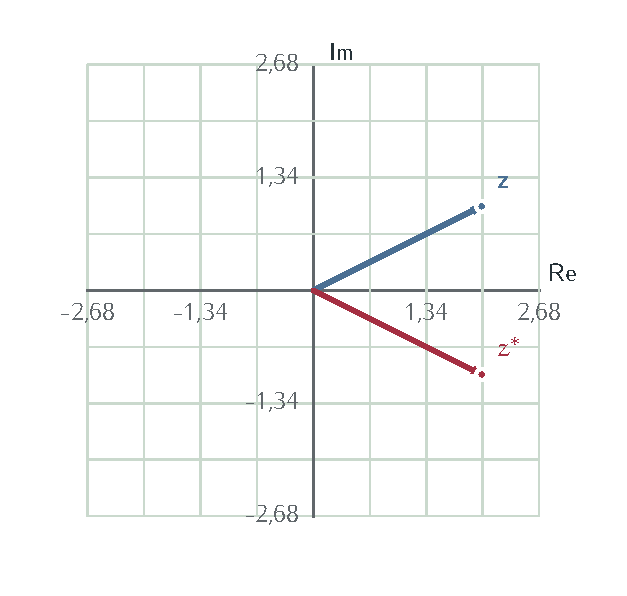
\includegraphics[width=\linewidth,height=94mm,keepaspectratio]{figure/f8719ed1304e49277.pdf}\FigureCaption{2.01 \(\cdot\) esempio 1 \(\cdot\) Piano complesso: numero e coniugato}\end{FigureBlock}

\phantomsection\label{c2-complessi-example-1-step-1}
\BookHeading{01 Individuare le due coordinate}

\MathBlock{007A003D00320020002B00200069003B0020005200650028007A0029003D0032003B00200049006D0028007A0029003D0031}{z=2\ +\ i;\allowbreak \ \operatorname{Re}(z)=2;\allowbreak \ \operatorname{Im}(z)=1}

La freccia parte dall'origine e termina nel punto indicato dalle due coordinate reali.\par


\phantomsection\label{c2-complessi-example-1-step-2}
\BookHeading{02 Applicare Pitagora}

\MathBlock{007C007A007C00B2003D00280032002900B2002B00280031002900B2003D0035003B0020007C007A007C003D221A003522480032002C0032003300360031}{|z|^{2}=(2)^{2}+(1)^{2}=5;\allowbreak \ |z|=\sqrt{5}\approx 2{,}2361}

Il modulo è una lunghezza e quindi è non negativo.\par


\phantomsection\label{c2-complessi-example-1-step-3}
\BookHeading{03 Determinare il quadrante e la fase}

\MathBlock{0063006F0073002003C6003D0032002F221A0035003B002000730069006E002003C6003D0031002F221A0035003B002003C6224800320036002C003500360035003100B0}{\cos \ \varphi =2/\sqrt{5};\allowbreak \ \sin \ \varphi =1/\sqrt{5};\allowbreak \ \varphi \approx 26{,}5651{}^{\circ} }
\MathBlock{007A003D221A003500280063006F0073002003C6002B0069002000730069006E002003C60029}{z=\sqrt{5}(\cos \ \varphi +i\ \sin \ \varphi )}

I segni di seno e coseno distinguono il quadrante; aggiungere \(360{}^{\circ} \) conserva lo stesso punto.\par


\phantomsection\label{c2-complessi-example-1-step-4}
\BookHeading{04 Costruire il coniugato}

\MathBlock{007A002A003D00320020221200200069003B0020007C007A002A007C00B2003D0035003B00200061007200670028007A002A00292248002D00320036002C003500360035003100B0}{z{}^{*}=2\ - \ i;\allowbreak \ |z{}^{*}|^{2}=5;\allowbreak \ \arg (z{}^{*})\approx -26{,}5651{}^{\circ} }

Coniugare conserva la coordinata reale e cambia il segno della coordinata immaginaria: la figura mostra la riflessione rispetto all'asse reale.\par


\phantomsection\label{c2-complessi-example-1-step-5}
\BookHeading{05 Separare il caso nullo}

\MathBlock{007A003D0030002021D20020005200650028007A0029003D0049006D0028007A0029003D0030003B0020007C007A007C003D0030003B00200061007200670028003000290020006E006F006E00200064006500660069006E00690074006F}{z=0\ \Rightarrow \ \operatorname{Re}(z)=\operatorname{Im}(z)=0;\allowbreak \ |z|=0;\allowbreak \ \arg (0)\ \text{non}\ \text{definito}}

L'origine appartiene al piano complesso, ma non individua un angolo.\par


\BookHeading{Interpretazione}

Il punto (2,1) e la forma polare descrivono lo stesso numero; il coniugio conserva \(\sqrt{5}\) e inverte la fase.\par


\Needspace{.36\textheight}\phantomsection\label{c2-complessi-example-2}
{\sffamily\small\color{Accent} ESEMPIO SVOLTO 2\par}
\BookHeading{Componente immaginaria negativa}
Dato \(z=1\) \(- \) i. Gli angoli sono orientati dall'asse reale positivo.\par


\BookHeading{Geometria e configurazione dell'esempio}
\begin{FigureBlock}\centering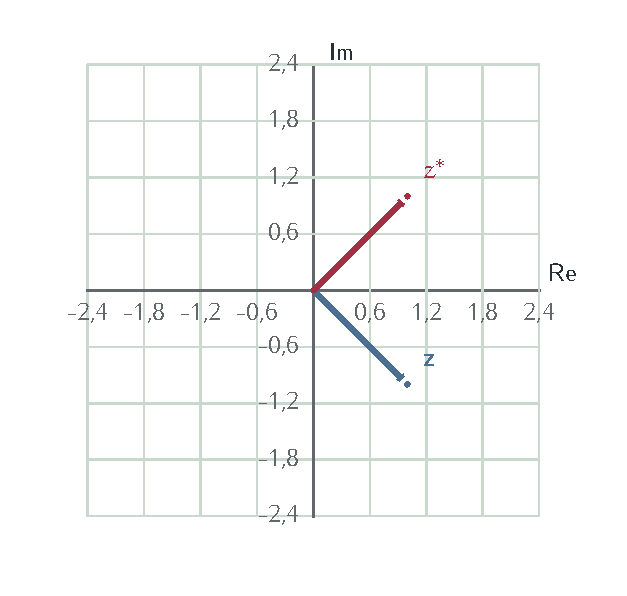
\includegraphics[width=\linewidth,height=94mm,keepaspectratio]{figure/f5202ebd1c1b2bb77.pdf}\FigureCaption{2.01 \(\cdot\) esempio 2 \(\cdot\) Piano complesso: numero e coniugato}\end{FigureBlock}

\phantomsection\label{c2-complessi-example-2-step-1}
\BookHeading{01 Individuare le due coordinate}

\MathBlock{007A003D00310020221200200069003B0020005200650028007A0029003D0031003B00200049006D0028007A0029003D002D0031}{z=1\ - \ i;\allowbreak \ \operatorname{Re}(z)=1;\allowbreak \ \operatorname{Im}(z)=-1}

La freccia parte dall'origine e termina nel punto indicato dalle due coordinate reali.\par


\phantomsection\label{c2-complessi-example-2-step-2}
\BookHeading{02 Applicare Pitagora}

\MathBlock{007C007A007C00B2003D00280031002900B2002B0028002D0031002900B2003D0032003B0020007C007A007C003D221A003222480031002C0034003100340032}{|z|^{2}=(1)^{2}+(-1)^{2}=2;\allowbreak \ |z|=\sqrt{2}\approx 1{,}4142}

Il modulo è una lunghezza e quindi è non negativo.\par


\phantomsection\label{c2-complessi-example-2-step-3}
\BookHeading{03 Determinare il quadrante e la fase}

\MathBlock{0063006F0073002003C6003D0031002F221A0032003B002000730069006E002003C6003D002D0031002F221A0032003B002003C62248002D0034003500B0}{\cos \ \varphi =1/\sqrt{2};\allowbreak \ \sin \ \varphi =-1/\sqrt{2};\allowbreak \ \varphi \approx -45{}^{\circ} }
\MathBlock{007A003D221A003200280063006F0073002003C6002B0069002000730069006E002003C60029}{z=\sqrt{2}(\cos \ \varphi +i\ \sin \ \varphi )}

I segni di seno e coseno distinguono il quadrante; aggiungere \(360{}^{\circ} \) conserva lo stesso punto.\par


\phantomsection\label{c2-complessi-example-2-step-4}
\BookHeading{04 Costruire il coniugato}

\MathBlock{007A002A003D00310020002B00200069003B0020007C007A002A007C00B2003D0032003B00200061007200670028007A002A002922480034003500B0}{z{}^{*}=1\ +\ i;\allowbreak \ |z{}^{*}|^{2}=2;\allowbreak \ \arg (z{}^{*})\approx 45{}^{\circ} }

Coniugare conserva la coordinata reale e cambia il segno della coordinata immaginaria: la figura mostra la riflessione rispetto all'asse reale.\par


\phantomsection\label{c2-complessi-example-2-step-5}
\BookHeading{05 Separare il caso nullo}

\MathBlock{007A003D0030002021D20020005200650028007A0029003D0049006D0028007A0029003D0030003B0020007C007A007C003D0030003B00200061007200670028003000290020006E006F006E00200064006500660069006E00690074006F}{z=0\ \Rightarrow \ \operatorname{Re}(z)=\operatorname{Im}(z)=0;\allowbreak \ |z|=0;\allowbreak \ \arg (0)\ \text{non}\ \text{definito}}

L'origine appartiene al piano complesso, ma non individua un angolo.\par


\BookHeading{Interpretazione}

Il segno della parte immaginaria distingue z dal suo coniugato; entrambi hanno modulo \(\sqrt{2}\).\par


\Needspace{7\baselineskip}
\BookHeading{Il passaggio successivo}
La rappresentazione cartesiana rende disponibili le componenti; sommandole e moltiplicandole potremo seguire cancellazioni, rotazioni e dilatazioni.\par


% Authoritative exercise source. Preserve all derivations and diagrams.

\ExerciseStart{G2.01}{Passare da componenti complesse a modulo e fase}{Guida esplicita}

\BookHeading{Problema, dati e obiettivo}

Dato \(z=-1+i\sqrt3\), calcolare modulo, fase principale nell’intervallo \((-\pi,\pi]\), coniugato, inverso e numero normalizzato. Spiegare geometricamente ogni operazione.

\ExTheory{\ExRef{c2-complessi}{2.01}}{Per \(z=a+ib\), il coniugato è \(z^*=a-ib\) e \(|z|=\sqrt{a^2+b^2}\). La fase si determina da seno, coseno e quadrante. Per \(z\ne0\), \(z^{-1}=z^*/|z|^2\); \(z/|z|\) appartiene al cerchio unitario.}

\ExPrediction{Il punto è nel secondo quadrante. Il coniugato sarà nel terzo; l’inverso avrà la stessa direzione del coniugato e una lunghezza reciproca di quella iniziale.}

\ExFigure{\begin{tikzpicture}[>=Stealth,exlabel]
\draw[exaxis] (-1.35,0)--(1.55,0) node[right] {$\operatorname{Re}$};\draw[exaxis] (0,-0.35)--(0,2.28205) node[above] {$\operatorname{Im}$};\draw[->,Accent,line width=1.1pt] (0,0)--(-1,1.73205) node[anchor=south west] {$ z $};
\end{tikzpicture}}{Il punto iniziale si trova nel secondo quadrante del piano complesso.}


\begin{ExTasks}

\item Identificare le componenti reali e immaginarie.

\item Calcolare il modulo quadro e il modulo.

\item Determinare il quadrante e la fase.

\item Costruire coniugato e inverso e verificarne il prodotto.

\item Normalizzare e controllare la lunghezza finale.

\end{ExTasks}

\ExSolution

\ExStep{Leggere le componenti}

La parte reale è \(a=-1\), la parte immaginaria è \(b=\sqrt3\). Il simbolo \(i\) soddisfa \(i^2=-1\); la coordinata verticale è il numero reale \(\sqrt3\).

\ExStep{Calcolare la lunghezza}

\ExEq{|z|^2&=(-1)^2+(\sqrt3)^2=1+3=4,\\|z|&=\sqrt4=2.}
Lo stesso risultato segue da \((-1-i\sqrt3)(-1+i\sqrt3)=1+3\), dopo cancellazione dei termini incrociati.

\ExStep{Scegliere l’angolo corretto}

\ExEq{\cos\varphi&=-1/2,\quad\sin\varphi=\sqrt3/2,\\\varphi&=2\pi/3=120^\circ,\qquad z=2e^{2\pi i/3}.}
Il rapporto \(b/a=-\sqrt3\) da solo ammetterebbe anche un angolo del quarto quadrante; il segno delle due coordinate seleziona il secondo.

\ExStep{Coniugare e invertire}

\ExEq{z^*&=-1-i\sqrt3,\\z^{-1}&=\frac{-1-i\sqrt3}{4}=-\frac14-i\frac{\sqrt3}{4},\\zz^{-1}&=\frac{(-1+i\sqrt3)(-1-i\sqrt3)}4=\frac{1+3}4=1.}
Il modulo dell’inverso è \(\sqrt{1/16+3/16}=1/2\).

\ExStep{Normalizzare}

\ExEq{\widehat z&=z/2=-\frac12+i\frac{\sqrt3}{2},\\|\widehat z|^2&=\frac14+\frac34=1.}
L’operazione conserva l’angolo di \(120^\circ\). Il vettore nullo non ammetterebbe questa divisione.

\par\noindent\begin{minipage}{\linewidth}
\ExFigure{\begin{tikzpicture}[>=Stealth,exlabel]
\draw[exaxis] (-1.35,0)--(1.55,0) node[right] {$\operatorname{Re}$};\draw[exaxis] (0,-2.08205)--(0,2.28205) node[above] {$\operatorname{Im}$};\draw[->,Accent,line width=1.1pt] (0,0)--(-1,1.73205) node[anchor=south west] {$ z $};\draw[->,Secondary,line width=1.1pt] (0,0)--(-1,-1.73205) node[anchor=north west] {$ z^* $};\draw[->,Ink,line width=1.1pt] (0,0)--(-0.25,-0.433013) node[anchor=north west] {$ z^{-1} $};
\end{tikzpicture}}{Il coniugio riflette rispetto all’asse reale; l’inversione aggiunge una variazione del modulo.}


\ExInterpret{Modulo e fase descrivono lo stesso punto delle coordinate cartesiane. Il piano complesso qui rappresenta un numero; negli stati quantistici ogni componente complessa avrà il proprio ruolo nella combinazione del vettore.}

\ExLab{Nella sezione 2.01 usare lo strumento del numero complesso e porre parte reale \(-1\), parte immaginaria \(\sqrt3\simeq1{,}73205\). Confrontare modulo e angolo; cambiare poi il segno della parte immaginaria. Se si inseriscono decimali, valutare l’errore rispetto ai risultati esatti.}


\end{minipage}

\Needspace{.43\textheight}
\section{Sommare e moltiplicare ampiezze}
\phantomsection\label{c2-prodotto-complesso}

{\sffamily\small\color{Ink!70} Riferimento alle slide: p. 11.\par}

{\sffamily\small\color{Ink!70} Laboratorio locale: \nolinkurl{index.html#capitolo-2/prodotto-complesso}\par}

\BookHeading{Definizioni e costruzione}
La somma combina contributi; la moltiplicazione può ruotare e dilatare il piano. Seguiamo separatamente queste due operazioni.\par

Per sommare due numeri complessi si sommano separatamente le parti reali e immaginarie. La costruzione punta-coda rappresenta questa operazione perché la traslazione della seconda freccia conserva le sue componenti. Le fasi relative determinano quanto la risultante sia lunga: contributi opposti possono cancellarsi.\par

Nel prodotto si distribuiscono tutti i termini e si sostituisce \(i^{2}\) con \(- 1\). In forma polare i moduli si moltiplicano e gli argomenti si sommano. Moltiplicare per i realizza quindi una rotazione di \(90{}^{\circ} \), mentre moltiplicare per un reale positivo realizza una dilatazione.\par


\MathBlock{00280078002B00690079002900280075002B006900760029003D0028007800752212007900760029002B0069002800780076002B007900750029002E}{(x+iy)(u+iv)=(xu- yv)+i(xv+yu).}

\BookHeading{Come leggere le figure}
Piano complesso; gli angoli sono fasi orientate.\par


\Needspace{.36\textheight}\phantomsection\label{c2-prodotto-complesso-example-1}
{\sffamily\small\color{Accent} ESEMPIO SVOLTO 1\par}
\BookHeading{Moltiplicazione per i}
Dati \(a=2\) + i, \(b=i\); confrontiamo a+b e ab.\par


\BookHeading{Geometria e configurazione dell'esempio}
\begin{FigureBlock}\centering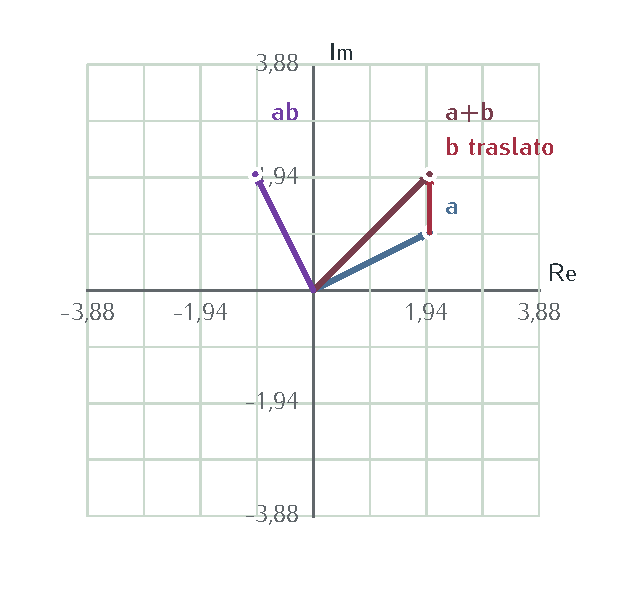
\includegraphics[width=\linewidth,height=94mm,keepaspectratio]{figure/f2c47dbfe9f52992c.pdf}\FigureCaption{2.02 \(\cdot\) esempio 1 \(\cdot\) Piano complesso: punta-coda e prodotto}\end{FigureBlock}

\phantomsection\label{c2-prodotto-complesso-example-1-step-1}
\BookHeading{01 Sommare le componenti}

\MathBlock{0061002B0062003D00280032002B0028003000290029002B006900280031002B0028003100290029003D00320020002B002000320069}{a+b=(2+(0))+i(1+(1))=2\ +\ 2i}

La freccia di b viene traslata alla punta di a; la risultante parte dall'origine.\par


\phantomsection\label{c2-prodotto-complesso-example-1-step-2}
\BookHeading{02 Distribuire i quattro prodotti}

\MathBlock{00610062003D003200B7002800300029002B00690028003200B7002800310029002B003100B70028003000290029002B006900B20028003100B70028003100290029}{ab=2\cdot (0)+i(2\cdot (1)+1\cdot (0))+i^{2}(1\cdot (1))}
\MathBlock{003D0028003022120028003100290029002B0069002800320029003D002D00310020002B002000320069}{=(0- (1))+i(2)=-1\ +\ 2i}

La sostituzione \(i^{2}=- 1\) dà la parte reale; i due termini con un solo i danno quella immaginaria.\par


\phantomsection\label{c2-prodotto-complesso-example-1-step-3}
\BookHeading{03 Leggere la trasformazione polare}

\MathBlock{007C00610062007C00B2003D007C0061007C00B2007C0062007C00B2003D003500B70031003D0035}{|ab|^{2}=|a|^{2}|b|^{2}=5\cdot 1=5}
\MathBlock{0061007200670028006100620029003D006100720067002800610029002B00610072006700280062002900200028006D006F0064002000330036003000B00029224800320036002C003500360035003100B0002B00280039003000B00029}{\arg (ab)=\arg (a)+\arg (b)\ (\bmod \ 360{}^{\circ} )\approx 26{,}5651{}^{\circ} +(90{}^{\circ} )}

Il prodotto somma le fasi e moltiplica i moduli. I due risultati si verificano dalle coordinate appena ottenute.\par


\phantomsection\label{c2-prodotto-complesso-example-1-step-4}
\BookHeading{04 Controllare la lunghezza della somma}

\MathBlock{007C0061002B0062007C00B2003D00280032002900B2002B00280032002900B2003D0038}{|a+b|^{2}=(2)^{2}+(2)^{2}=8}
\MathBlock{007C0061002B0062007C003D221A0038003B0020007C0061007C002B007C0062007C003D221A0035002B0031}{|a+b|=\sqrt{8};\allowbreak \ |a|+|b|=\sqrt{5}+1}

I moduli della somma e dei singoli contributi dipendono dall'angolo fra le frecce; in questo caso \(\sqrt{8}<\sqrt{5}+1\).\par


\BookHeading{Interpretazione}

Il fattore i conserva il modulo \(\sqrt{5}\) e ruota a di \(90{}^{\circ} \); la somma a+i raggiunge invece il punto (2,2).\par


\Needspace{.36\textheight}\phantomsection\label{c2-prodotto-complesso-example-2}
{\sffamily\small\color{Accent} ESEMPIO SVOLTO 2\par}
\BookHeading{Cancellazione nella somma}
Dati \(a=1\) + i, \(b=-1\) \(- \) i; confrontiamo a+b e ab.\par


\BookHeading{Geometria e configurazione dell'esempio}
\begin{FigureBlock}\centering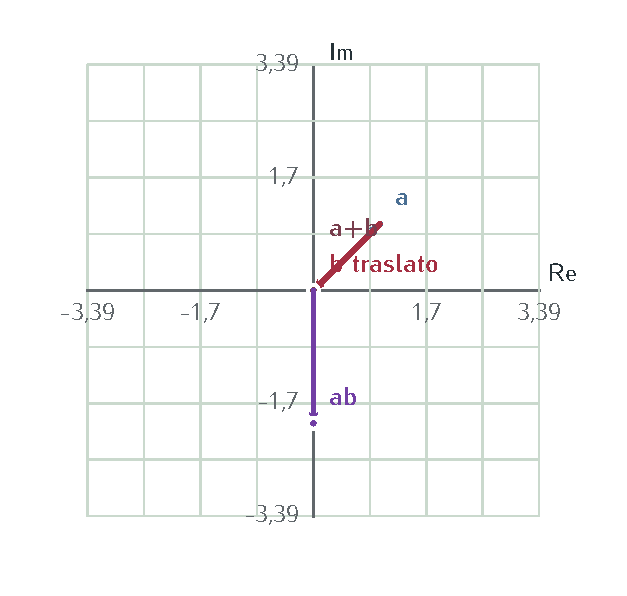
\includegraphics[width=\linewidth,height=94mm,keepaspectratio]{figure/fa2630e4447821995.pdf}\FigureCaption{2.02 \(\cdot\) esempio 2 \(\cdot\) Piano complesso: punta-coda e prodotto}\end{FigureBlock}

\phantomsection\label{c2-prodotto-complesso-example-2-step-1}
\BookHeading{01 Sommare le componenti}

\MathBlock{0061002B0062003D00280031002B0028002D003100290029002B006900280031002B0028002D003100290029003D0030}{a+b=(1+(-1))+i(1+(-1))=0}

La freccia di b viene traslata alla punta di a; la risultante parte dall'origine.\par


\phantomsection\label{c2-prodotto-complesso-example-2-step-2}
\BookHeading{02 Distribuire i quattro prodotti}

\MathBlock{00610062003D003100B70028002D00310029002B00690028003100B70028002D00310029002B003100B70028002D003100290029002B006900B20028003100B70028002D003100290029}{ab=1\cdot (-1)+i(1\cdot (-1)+1\cdot (-1))+i^{2}(1\cdot (-1))}
\MathBlock{003D0028002D003122120028002D003100290029002B00690028002D00320029003D002D00320069}{=(-1- (-1))+i(-2)=-2i}

La sostituzione \(i^{2}=- 1\) dà la parte reale; i due termini con un solo i danno quella immaginaria.\par


\phantomsection\label{c2-prodotto-complesso-example-2-step-3}
\BookHeading{03 Leggere la trasformazione polare}

\MathBlock{007C00610062007C00B2003D007C0061007C00B2007C0062007C00B2003D003200B70032003D0034}{|ab|^{2}=|a|^{2}|b|^{2}=2\cdot 2=4}
\MathBlock{0061007200670028006100620029003D006100720067002800610029002B00610072006700280062002900200028006D006F0064002000330036003000B0002922480034003500B0002B0028002D00310033003500B00029}{\arg (ab)=\arg (a)+\arg (b)\ (\bmod \ 360{}^{\circ} )\approx 45{}^{\circ} +(-135{}^{\circ} )}

Il prodotto somma le fasi e moltiplica i moduli. I due risultati si verificano dalle coordinate appena ottenute.\par


\phantomsection\label{c2-prodotto-complesso-example-2-step-4}
\BookHeading{04 Controllare la lunghezza della somma}

\MathBlock{007C0061002B0062007C00B2003D00280030002900B2002B00280030002900B2003D0030}{|a+b|^{2}=(0)^{2}+(0)^{2}=0}
\MathBlock{007C0061002B0062007C003D00300020006D0065006E0074007200650020007C0061007C002B007C0062007C003D0032221A0032}{|a+b|=0\ \text{mentre}\ |a|+|b|=2\sqrt{2}}

Contributi opposti hanno una risultante nulla, pur avendo singolarmente modulo positivo.\par


\BookHeading{Interpretazione}

La somma è zero perché i due contributi sono opposti. Il prodotto vale \(- 2i\): la cancellazione della somma non implica l'annullamento del prodotto.\par


\Needspace{7\baselineskip}
\BookHeading{Il passaggio successivo}
Le somme di contributi verranno ora generalizzate ai vettori: scegliere una base significa fissare le direzioni che ricostruiscono ogni ingresso.\par


% Authoritative exercise source. Preserve all derivations and diagrams.

\ExerciseStart{G2.02}{Sommare e moltiplicare due ampiezze}{Guida esplicita}

\BookHeading{Problema, dati e obiettivo}

Siano \(z=1+i\) e \(w=1-i\). Calcolare \(z+w\), \(zw\) e \(z^2\). Interpretare somma e prodotto nel piano complesso e confrontare le lunghezze ottenute.

\ExTheory{\ExRef{c2-prodotto-complesso}{2.02}}{La somma si esegue componente per componente. Il prodotto si sviluppa distributivamente usando \(i^2=-1\). In forma polare \((r e^{i\theta})(s e^{i\phi})=rs e^{i(\theta+\phi)}\): i moduli si moltiplicano e le fasi si sommano.}

\ExPrediction{I due numeri sono coniugati: hanno uguale lunghezza e angoli opposti. Prevedere la direzione del loro prodotto e confrontarla con quella della loro somma.}

\ExFigure{\begin{tikzpicture}[>=Stealth,exlabel]
\draw[exaxis] (-0.35,0)--(1.55,0) node[right] {$\operatorname{Re}$};\draw[exaxis] (0,-1.35)--(0,1.55) node[above] {$\operatorname{Im}$};\draw[->,Accent,line width=1.1pt] (0,0)--(1,1) node[anchor=south west] {$ z $};\draw[->,Secondary,line width=1.1pt] (0,0)--(1,-1) node[anchor=north west] {$ w $};
\end{tikzpicture}}{Fattori e addendi hanno uguale modulo e fasi opposte.}


\begin{ExTasks}

\item Calcolare la somma.

\item Sviluppare tutti i termini del prodotto.

\item Ricavare i moduli e gli angoli dei fattori.

\item Confermare il prodotto in forma polare.

\item Calcolare il quadrato di z e confrontare le due trasformazioni.

\end{ExTasks}

\ExSolution

\ExStep{Sommare le componenti}

\ExEq{z+w&=(1+1)+i(1-1)=2.}
La costruzione punta-coda porta dal punto \((1,1)\) al punto \((2,0)\).

\ExStep{Svolgere il prodotto}

\ExEq{zw&=(1+i)(1-i)=1\cdot1+1(-i)+i\cdot1+i(-i)\\&=1-i+i-i^2=1+1=2.}

\ExStep{Passare alla forma polare}

\ExEq{|z|=|w|&=\sqrt{1^2+1^2}=\sqrt2,\\\arg z&=\pi/4,\quad\arg w=-\pi/4.}
I quadranti sono rispettivamente il primo e il quarto.

\ExStep{Interpretare il prodotto come trasformazione}

\ExEq{zw&=(\sqrt2 e^{i\pi/4})(\sqrt2 e^{-i\pi/4})
=2e^0=2.}
Moltiplicare z per w applica una rotazione di \(-45^\circ\) e una dilatazione di fattore \(\sqrt2\).

\ExStep{Confrontare con il quadrato}

\ExEq{z^2&=(1+i)(1+i)=1+i+i+i^2=2i,\\z^2&=(\sqrt2)^2e^{i(\pi/4+\pi/4)}=2e^{i\pi/2}=2i.}
Il modulo è ancora 2; la direzione è verticale perché la rotazione ora è \(+45^\circ\). L’uguaglianza numerica fra somma e prodotto nel primo confronto dipende dai dati scelti.

\par\noindent\begin{minipage}{\linewidth}
\ExFigure{\begin{tikzpicture}[>=Stealth,exlabel]
\draw[exaxis] (-0.35,0)--(2.55,0) node[right] {$\operatorname{Re}$};\draw[exaxis] (0,-0.35)--(0,2.55) node[above] {$\operatorname{Im}$};\draw[->,Accent,line width=1.1pt] (0,0)--(2,0) node[anchor=south west] {$ zw $};\draw[->,Secondary,line width=1.1pt] (0,0)--(0,2) node[anchor=south west] {$ z^2 $};
\end{tikzpicture}}{I due prodotti hanno modulo 2 e fasi rispettivamente 0 e \(\pi/2\).}


\ExInterpret{La somma combina contributi mediante traslazione dei segmenti; il prodotto trasforma un contributo mediante rotazione e dilatazione. Questa distinzione sarà necessaria per seguire interferenza e porte di fase.}

\ExLab{Nella sezione 2.02 impostare i due numeri nello strumento esplorativo. Confrontare somma e prodotto, poi sostituire w con z. Controllare che la costruzione geometrica e il calcolo distributivo descrivano lo stesso risultato.}


\end{minipage}

\Needspace{.43\textheight}
\section{Vettori, combinazioni e basi}
\phantomsection\label{c2-basi}

{\sffamily\small\color{Ink!70} Riferimento alle slide: p. 33.\par}

{\sffamily\small\color{Ink!70} Laboratorio locale: \nolinkurl{index.html#capitolo-2/basi}\par}

\BookHeading{Definizioni e costruzione}
Le coordinate indicano i coefficienti con cui una base ricostruisce il vettore. La scelta di assi obliqui rende visibile questa dipendenza.\par

Una base del piano contiene due vettori linearmente indipendenti: nessuno è un multiplo dell'altro. Ogni vettore del piano ammette allora un'unica espressione come loro combinazione. Le coordinate sono i coefficienti di quella combinazione; la freccia geometrica è ricostruita sommando i due contributi.\par

La matrice \(B\) è qui una tabella che raccoglie i vettori della base come colonne. Scrivere \(Bc=v\) abbrevia la combinazione delle colonne con coefficienti \(c_{1},\allowbreak c_{2}\). Per \(B=\)\(\begin{pmatrix}a&b\\c&d\end{pmatrix}\), il determinante è \(ad- bc\); misura l'area orientata del parallelogramma delle due colonne. Se è diverso da zero esse sono indipendenti. Se è zero, alcuni vettori possono risultare irraggiungibili e quelli raggiungibili possono avere più descrizioni.\par


\MathBlock{0076003D0063208100622081002B0063208200622082003D00420063003B0020006C006500200063006F006C006F006E006E00650020006400690020004200200073006F006E006F002000622081002C00622082002E}{v=c_{1}b_{1}+c_{2}b_{2}=Bc;\allowbreak \ \text{le}\ \text{colonne}\ \text{di}\ B\ \text{sono}\ b_{1},\allowbreak b_{2}.}

\BookHeading{Come leggere le figure}
Piano reale \(R^{2}\); vettore e coordinate sono oggetti distinti.\par


\Needspace{.36\textheight}\phantomsection\label{c2-basi-example-1}
{\sffamily\small\color{Accent} ESEMPIO SVOLTO 1\par}
\BookHeading{Coordinate in una base obliqua}
Dati \(b_{1}=(1{,}0)\), \(b_{2}=(1{,}1)\), \(B=\)\(\begin{pmatrix}1&1\\0&1\end{pmatrix}\), \(v=(3\); \(2)^{T}\).\par


\BookHeading{Geometria e configurazione dell'esempio}
\begin{FigureBlock}\centering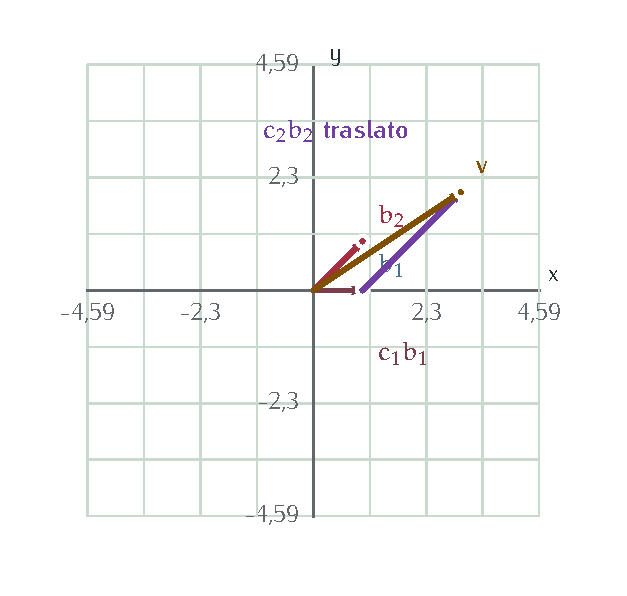
\includegraphics[width=\linewidth,height=94mm,keepaspectratio]{figure/f341afc6c29ff8c99.pdf}\FigureCaption{2.03 \(\cdot\) esempio 1 \(\cdot\) Base e ricostruzione punta-coda}\end{FigureBlock}

\phantomsection\label{c2-basi-example-1-step-1}
\BookHeading{01 Ricostruire il vettore}

\MathBlock{00420063003D0063208100280031002C00300029002B0063208200280031002C00310029003D002800632081002B003100632082002C006320820029003D00280033003B0020003200291D40}{Bc=c_{1}(1{,}0)+c_{2}(1{,}1)=(c_{1}+1c_{2},\allowbreak c_{2})=(3;\allowbreak \ 2)^{T}}

Le coordinate cercate sono i coefficienti \(c_{1},\allowbreak c_{2}\).\par


\phantomsection\label{c2-basi-example-1-step-2}
\BookHeading{02 Risolvere il sistema}

\MathBlock{00632082003D0032003B002000632081003D00332212003100B70032003D0031003B0020005B0076005D0042003D00280031003B0020003200291D40}{c_{2}=2;\allowbreak \ c_{1}=3- 1\cdot 2=1;\allowbreak \ [v]B=(1;\allowbreak \ 2)^{T}}

La seconda equazione determina \(c_{2}\); la prima determina poi \(c_{1}\) in modo unico.\par


\phantomsection\label{c2-basi-example-1-step-3}
\BookHeading{03 Verificare la somma}

\MathBlock{0063208100622081003D00280031003B0020003000291D40003B00200063208200622082003D00280032003B0020003200291D40}{c_{1}b_{1}=(1;\allowbreak \ 0)^{T};\allowbreak \ c_{2}b_{2}=(2;\allowbreak \ 2)^{T}}
\MathBlock{0063208100622081002B0063208200622082003D00280033003B0020003200291D40}{c_{1}b_{1}+c_{2}b_{2}=(3;\allowbreak \ 2)^{T}}

I contributi hanno le direzioni della base, mentre la loro somma coincide con v.\par


\phantomsection\label{c2-basi-example-1-step-4}
\BookHeading{04 Controllare l'indipendenza}

\MathBlock{00640065007400200042003D003100B700312212003100B70030003D003122600030}{\det \ B=1\cdot 1- 1\cdot 0=1\ne 0}
\MathBlock{0043006F006E002000622082003D003200622081003A00200063208100622081002B0063208200622082003D002800632081002B003200632082002C00300029}{\text{Con}\ b_{2}=2b_{1}:\ c_{1}b_{1}+c_{2}b_{2}=(c_{1}+2c_{2}{,}0)}

Nel caso dipendente una componente verticale non nulla sarebbe irraggiungibile; una freccia orizzontale avrebbe più coppie di coefficienti.\par


\BookHeading{Interpretazione}

Le coordinate nella base scelta sono (1,2). Il secondo contributo fornisce tutta la componente verticale; il primo completa quella orizzontale.\par


\Needspace{.36\textheight}\phantomsection\label{c2-basi-example-2}
{\sffamily\small\color{Accent} ESEMPIO SVOLTO 2\par}
\BookHeading{Base più inclinata}
Dati \(b_{1}=(1{,}0)\), \(b_{2}=(2{,}1)\), \(B=\)\(\begin{pmatrix}1&2\\0&1\end{pmatrix}\), \(v=(5\); \(2)^{T}\).\par


\BookHeading{Geometria e configurazione dell'esempio}
\begin{FigureBlock}\centering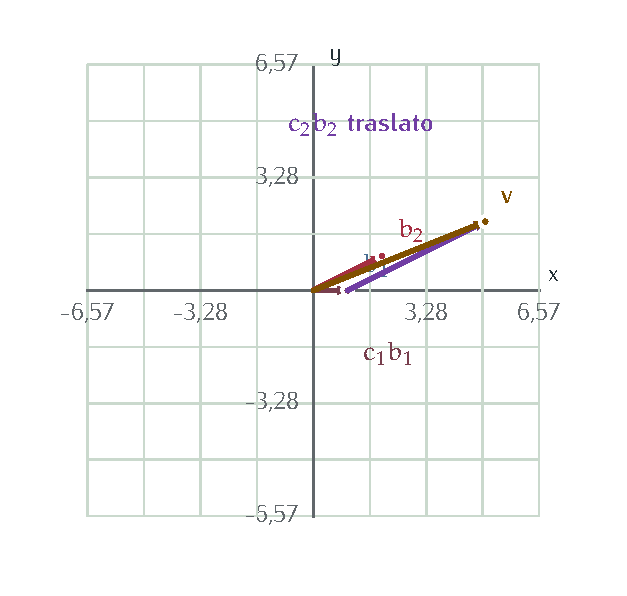
\includegraphics[width=\linewidth,height=94mm,keepaspectratio]{figure/fa0a998fb9b87cc03.pdf}\FigureCaption{2.03 \(\cdot\) esempio 2 \(\cdot\) Base e ricostruzione punta-coda}\end{FigureBlock}

\phantomsection\label{c2-basi-example-2-step-1}
\BookHeading{01 Ricostruire il vettore}

\MathBlock{00420063003D0063208100280031002C00300029002B0063208200280032002C00310029003D002800632081002B003200632082002C006320820029003D00280035003B0020003200291D40}{Bc=c_{1}(1{,}0)+c_{2}(2{,}1)=(c_{1}+2c_{2},\allowbreak c_{2})=(5;\allowbreak \ 2)^{T}}

Le coordinate cercate sono i coefficienti \(c_{1},\allowbreak c_{2}\).\par


\phantomsection\label{c2-basi-example-2-step-2}
\BookHeading{02 Risolvere il sistema}

\MathBlock{00632082003D0032003B002000632081003D00352212003200B70032003D0031003B0020005B0076005D0042003D00280031003B0020003200291D40}{c_{2}=2;\allowbreak \ c_{1}=5- 2\cdot 2=1;\allowbreak \ [v]B=(1;\allowbreak \ 2)^{T}}

La seconda equazione determina \(c_{2}\); la prima determina poi \(c_{1}\) in modo unico.\par


\phantomsection\label{c2-basi-example-2-step-3}
\BookHeading{03 Verificare la somma}

\MathBlock{0063208100622081003D00280031003B0020003000291D40003B00200063208200622082003D00280034003B0020003200291D40}{c_{1}b_{1}=(1;\allowbreak \ 0)^{T};\allowbreak \ c_{2}b_{2}=(4;\allowbreak \ 2)^{T}}
\MathBlock{0063208100622081002B0063208200622082003D00280035003B0020003200291D40}{c_{1}b_{1}+c_{2}b_{2}=(5;\allowbreak \ 2)^{T}}

I contributi hanno le direzioni della base, mentre la loro somma coincide con v.\par


\phantomsection\label{c2-basi-example-2-step-4}
\BookHeading{04 Controllare l'indipendenza}

\MathBlock{00640065007400200042003D003100B700312212003200B70030003D003122600030}{\det \ B=1\cdot 1- 2\cdot 0=1\ne 0}
\MathBlock{0043006F006E002000622082003D003200622081003A00200063208100622081002B0063208200622082003D002800632081002B003200632082002C00300029}{\text{Con}\ b_{2}=2b_{1}:\ c_{1}b_{1}+c_{2}b_{2}=(c_{1}+2c_{2}{,}0)}

Nel caso dipendente una componente verticale non nulla sarebbe irraggiungibile; una freccia orizzontale avrebbe più coppie di coefficienti.\par


\BookHeading{Interpretazione}

Le coordinate nella base scelta sono (1,2). Il secondo contributo fornisce tutta la componente verticale; il primo completa quella orizzontale.\par


\Needspace{7\baselineskip}
\BookHeading{Il passaggio successivo}
Una base assegna coordinate a un vettore. Per confrontarne le lunghezze occorre specificare la norma, che resta indipendente dalla particolare scrittura in una base.\par


\Needspace{.43\textheight}
\section{Lunghezza e normalizzazione}
\phantomsection\label{c2-norma}

{\sffamily\small\color{Ink!70} Riferimento alle slide: p. 45.\par}

{\sffamily\small\color{Ink!70} Laboratorio locale: \nolinkurl{index.html#capitolo-2/norma}\par}

\BookHeading{Definizioni e costruzione}
Prima di usare un vettore come direzione unitaria ne calcoliamo la norma. Dividere per la lunghezza conserva la direzione.\par

La norma euclidea estende il teorema di Pitagora a un numero arbitrario di componenti. Per una componente complessa x+iy il contributo è \(x^{2}+y^{2}\), ossia il modulo quadro. Sommando questi contributi si ottiene un numero reale non negativo.\par

La divisione per la norma moltiplica tutte le componenti per lo stesso fattore positivo. La direzione e le proporzioni interne rimangono invariate. Il vettore nullo richiede un trattamento separato, poiché la sua norma è zero e non permette di costruire una direzione unitaria.\par


\MathBlock{20160076201600B2003D03A32C7C007C00762C7C007C00B2003B00200075003D0076002F20160076201600200070006500720020007622600030002E}{\Vert v\Vert ^{2}=\sum _{j}|v_{j}|^{2};\allowbreak \ u=v/\Vert v\Vert \ \text{per}\ v\ne 0.}

\BookHeading{Come leggere le figure}
Vettori reali nel primo esempio, componenti complesse nel secondo.\par


\Needspace{.36\textheight}\phantomsection\label{c2-norma-example-1}
{\sffamily\small\color{Accent} ESEMPIO SVOLTO 1\par}
\BookHeading{Il triangolo 3--4--5}
Dato \(u=(3\); \(4)^{T}\).\par


\BookHeading{Geometria e configurazione dell'esempio}
\begin{FigureBlock}\centering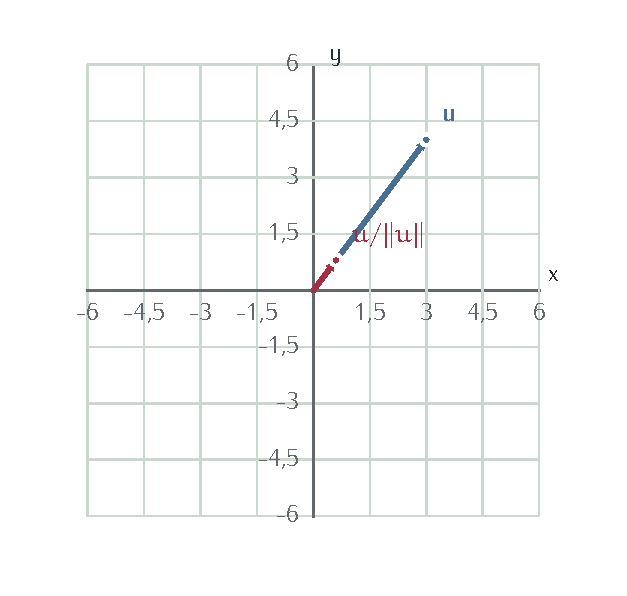
\includegraphics[width=\linewidth,height=94mm,keepaspectratio]{figure/ff8298f9f56719a17.pdf}\FigureCaption{2.04 \(\cdot\) esempio 1 \(\cdot\) Una direzione con due lunghezze}\end{FigureBlock}

\phantomsection\label{c2-norma-example-1-step-1}
\BookHeading{01 Calcolare i moduli quadri}

\MathBlock{007C00750031007C00B2003D00280033002900B2002B00280030002900B2003D0039}{|u1|^{2}=(3)^{2}+(0)^{2}=9}
\MathBlock{007C00750032007C00B2003D00280034002900B2002B00280030002900B2003D00310036}{|u2|^{2}=(4)^{2}+(0)^{2}=16}

Ogni componente complessa contribuisce mediante entrambe le sue coordinate reali.\par


\phantomsection\label{c2-norma-example-1-step-2}
\BookHeading{02 Sommare e prendere la radice}

\MathBlock{20160075201600B2003D0039002B00310036003D00320035003B0020201600752016003D221A0032003522480035}{\Vert u\Vert ^{2}=9+16=25;\allowbreak \ \Vert u\Vert =\sqrt{25}\approx 5}

Il totale è positivo perché u non è nullo.\par


\phantomsection\label{c2-norma-example-1-step-3}
\BookHeading{03 Dividere ogni componente}

\MathBlock{0065003D0075002F221A00320035224800280030002C0036003B00200030002C003800291D40}{e=u/\sqrt{25}\approx (0{,}6;\allowbreak \ 0{,}8)^{T}}
\MathBlock{20160065201600B2003D00280039002B003100360029002F00320035003D0031}{\Vert e\Vert ^{2}=(9+16)/25=1}

Il medesimo fattore positivo conserva la direzione del vettore e le fasi delle componenti.\par


\phantomsection\label{c2-norma-example-1-step-4}
\BookHeading{04 Separare il caso nullo}

\MathBlock{0075003D0030002021D20020201600752016003D0030003B00200075002F2016007520160020006E006F006E00200064006500660069006E00690074006F}{u=0\ \Rightarrow \ \Vert u\Vert =0;\allowbreak \ u/\Vert u\Vert \ \text{non}\ \text{definito}}

L'origine non individua una direzione da rendere unitaria.\par


\BookHeading{Interpretazione}

La lunghezza 5 diventa 1; le coordinate (3/5,4/5) conservano il rapporto 3:4.\par


\Needspace{.36\textheight}\phantomsection\label{c2-norma-example-2}
{\sffamily\small\color{Accent} ESEMPIO SVOLTO 2\par}
\BookHeading{Normalizzare componenti complesse}
Dato \(u=(1\) + i; \(2i)^{T}\).\par


\BookHeading{Geometria e configurazione dell'esempio}
\begin{FigureBlock}\begin{minipage}[t]{.485\linewidth}\centering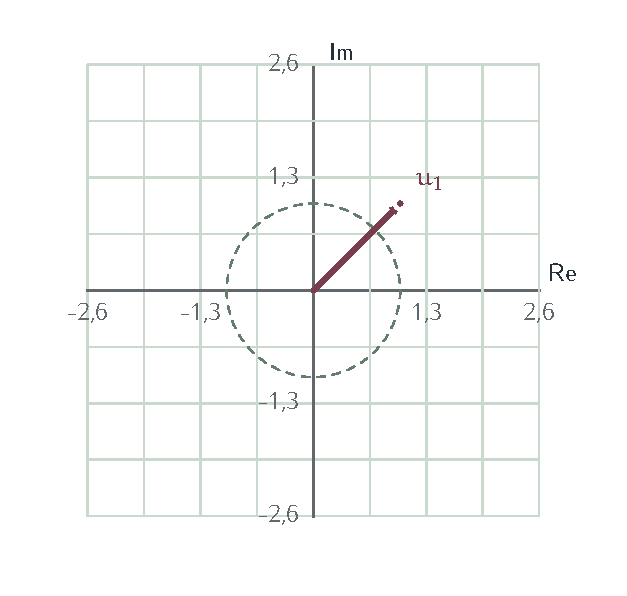
\includegraphics[width=\linewidth,height=63mm,keepaspectratio]{figure/f45f2738707df6198.pdf}\par{\sffamily\footnotesize \(u_{1}\)\par}\end{minipage}\hfill\begin{minipage}[t]{.485\linewidth}\centering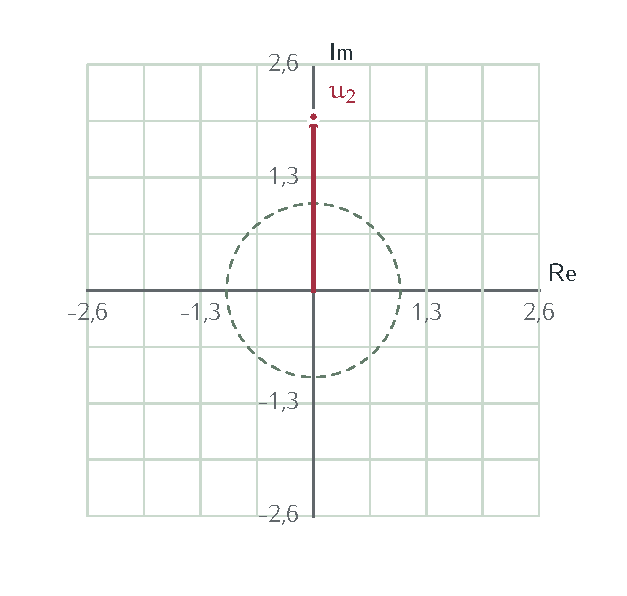
\includegraphics[width=\linewidth,height=63mm,keepaspectratio]{figure/f7c4e0ba32685ac54.pdf}\par{\sffamily\footnotesize \(u_{2}\)\par}\end{minipage}\FigureCaption{2.04 \(\cdot\) esempio 2 \(\cdot\) Componenti prima e dopo la normalizzazione}\end{FigureBlock}
\begin{FigureBlock}\begin{minipage}[t]{.485\linewidth}\centering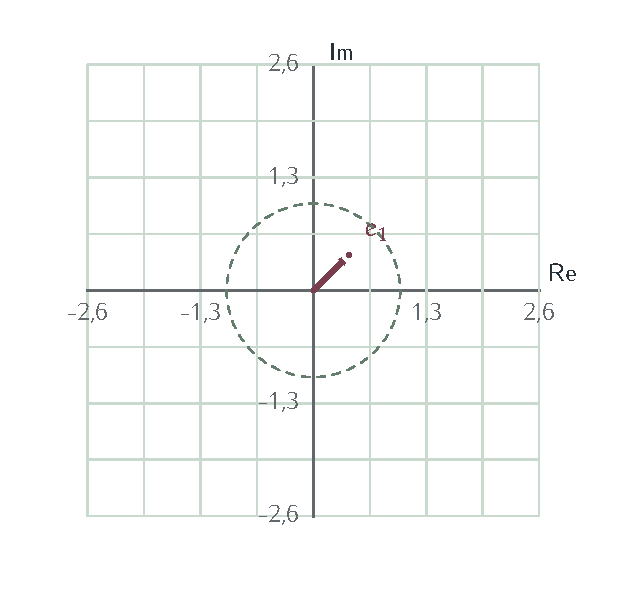
\includegraphics[width=\linewidth,height=63mm,keepaspectratio]{figure/f8b84a564def9b614.pdf}\par{\sffamily\footnotesize \(e_{1}\)\par}\end{minipage}\hfill\begin{minipage}[t]{.485\linewidth}\centering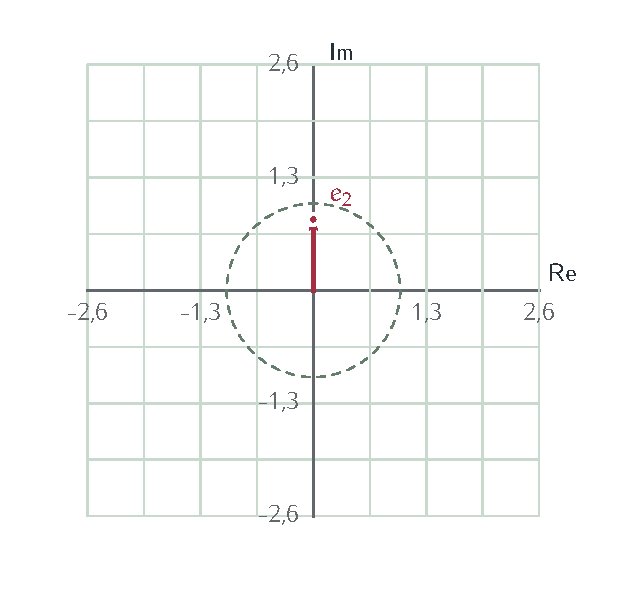
\includegraphics[width=\linewidth,height=63mm,keepaspectratio]{figure/f2976d8da2452c83e.pdf}\par{\sffamily\footnotesize \(e_{2}\)\par}\end{minipage}\FigureCaption{2.04 \(\cdot\) esempio 2 \(\cdot\) Componenti prima e dopo la normalizzazione}\end{FigureBlock}

\phantomsection\label{c2-norma-example-2-step-1}
\BookHeading{01 Calcolare i moduli quadri}

\MathBlock{007C00750031007C00B2003D00280031002900B2002B00280031002900B2003D0032}{|u1|^{2}=(1)^{2}+(1)^{2}=2}
\MathBlock{007C00750032007C00B2003D00280030002900B2002B00280032002900B2003D0034}{|u2|^{2}=(0)^{2}+(2)^{2}=4}

Ogni componente complessa contribuisce mediante entrambe le sue coordinate reali.\par


\phantomsection\label{c2-norma-example-2-step-2}
\BookHeading{02 Sommare e prendere la radice}

\MathBlock{20160075201600B2003D0032002B0034003D0036003B0020201600752016003D221A003622480032002C0034003400390035}{\Vert u\Vert ^{2}=2+4=6;\allowbreak \ \Vert u\Vert =\sqrt{6}\approx 2{,}4495}

Il totale è positivo perché u non è nullo.\par


\phantomsection\label{c2-norma-example-2-step-3}
\BookHeading{03 Dividere ogni componente}

\MathBlock{0065003D0075002F221A0036224800280030002C00340030003800320020002B00200030002C00340030003800320069003B00200030002C0038003100360035006900291D40}{e=u/\sqrt{6}\approx (0{,}4082\ +\ 0{,}4082i;\allowbreak \ 0{,}8165i)^{T}}
\MathBlock{20160065201600B2003D00280032002B00340029002F0036003D0031}{\Vert e\Vert ^{2}=(2+4)/6=1}

Il medesimo fattore positivo conserva la direzione del vettore e le fasi delle componenti.\par


\phantomsection\label{c2-norma-example-2-step-4}
\BookHeading{04 Separare il caso nullo}

\MathBlock{0075003D0030002021D20020201600752016003D0030003B00200075002F2016007520160020006E006F006E00200064006500660069006E00690074006F}{u=0\ \Rightarrow \ \Vert u\Vert =0;\allowbreak \ u/\Vert u\Vert \ \text{non}\ \text{definito}}

L'origine non individua una direzione da rendere unitaria.\par


\BookHeading{Interpretazione}

La norma è \(\sqrt{6}\): entrambi i piani delle componenti vengono riscalati dello stesso fattore \(1/\sqrt{6}\).\par


\Needspace{7\baselineskip}
\BookHeading{Il passaggio successivo}
La somma dei moduli quadri calcola una lunghezza. Il prodotto interno estenderà lo stesso coniugio al confronto fra due vettori e riconoscerà l'ortogonalità.\par


% Authoritative exercise source. Preserve all derivations and diagrams.

\ExerciseStart{G2.03}{Ricostruire un vettore e normalizzarlo}{Guida esplicita}

\BookHeading{Problema, dati e obiettivo}

Nello spazio \(\mathbb C^2\) con base canonica \(e_1=(1,0)^T\), \(e_2=(0,1)^T\), ricostruire il vettore \(v=(1+i)e_1+2e_2\), calcolarne la norma e normalizzarlo. Tenere distinti il vettore e i piani delle sue due componenti.

\ExTheory{\ExRef{c2-basi}{2.03}; \ExRef{c2-norma}{2.04}}{Il prodotto interno coniuga il primo argomento: \(\langle v|w\rangle=\sum_jv_j^*w_j\). La norma è \(\sqrt{\langle v|v\rangle}\). Per \(v\ne0\), il vettore \(u=v/\|v\|\) ha norma uno.}

\ExPrediction{La normalizzazione applica lo stesso fattore reale positivo a entrambe le componenti. Le loro fasi e il rapporto fra le loro lunghezze rimangono invariati.}

\ExFigure{\begin{tikzpicture}[>=Stealth,exlabel]
\draw[exaxis] (-0.35,0)--(2.55,0) node[right] {$\operatorname{Re}$};\draw[exaxis] (0,-0.35)--(0,1.55) node[above] {$\operatorname{Im}$};\draw[->,Accent,line width=1.1pt] (0,0)--(1,1) node[anchor=south west] {$ v_1 $};\draw[->,Secondary,line width=1.1pt] (0,0)--(2,0) node[anchor=south west] {$ v_2 $};
\end{tikzpicture}}{Confronto delle due componenti nello stesso riferimento complesso. Le frecce sono numeri diversi del vettore, non assi di \(\mathbb C^2\).}


\begin{ExTasks}

\item Svolgere i due prodotti scalare-vettore.

\item Sommare le componenti e scrivere il coniugato trasposto.

\item Calcolare la norma al quadrato.

\item Dividere tutte le componenti per la norma.

\item Controllare la norma finale e interpretare i quattro dati reali.

\end{ExTasks}

\ExSolution

\ExStep{Ricostruire il vettore}

\ExEq{(1+i)e_1&=\colv{1+i\\0},\quad2e_2=\colv{0\\2},\\v&=\colv{1+i+0\\0+2}=\colv{1+i\\2}.}

\ExStep{Coniugare e trasporre}

\ExEq{v^\dagger&=(1-i,\ 2).}
Il coniugio cambia il segno della parte immaginaria e la trasposizione cambia la colonna in riga.

\ExStep{Calcolare la norma}

\ExEq{v^\dagger v&=(1-i)(1+i)+2\cdot2\\&=1+i-i-i^2+4=2+4=6,\\\|v\|&=\sqrt6.}

\ExStep{Normalizzare entrambe le componenti}

\ExEq{u&=\frac1{\sqrt6}\colv{1+i\\2}.}
Le lunghezze delle componenti sono \(\sqrt2/\sqrt6=1/\sqrt3\) e \(2/\sqrt6=\sqrt{2/3}\).

\ExStep{Verificare e interpretare}

\ExEq{u^\dagger u&=\frac{(1-i)(1+i)+4}{6}=\frac26+\frac46=1.}
Il vettore v richiede quattro coordinate reali, \((1,1,2,0)\); la sua norma è la radice di \(1^2+1^2+2^2+0^2=6\). Due piani complessi visualizzano le componenti separatamente; un singolo piano ordinario non rappresenta tutto \(\mathbb C^2\).

\par\noindent\begin{minipage}{\linewidth}
\ExFigure{\begin{tikzpicture}[>=Stealth,exlabel]
\draw[exaxis] (-0.35,0)--(1.55,0) node[right] {$\operatorname{Re}$};\draw[exaxis] (0,-0.35)--(0,1.05) node[above] {$\operatorname{Im}$};\draw[->,Accent,line width=1.1pt] (0,0)--(0.408248,0.408248) node[anchor=south west] {$ u_1 $};\draw[->,Secondary,line width=1.1pt] (0,0)--(0.816497,0) node[anchor=south west] {$ u_2 $};
\end{tikzpicture}}{Componenti dopo la divisione comune per \(\sqrt6\). Le due lunghezze quadrate sommano a uno.}


\ExInterpret{La norma del vettore combina i moduli quadri di tutte le componenti. Questa normalizzazione prepara la descrizione degli stati che sarà introdotta nelle sezioni dedicate alla misura.}

\ExLab{Nelle sezioni 2.03–2.04 confrontare ricostruzione e normalizzazione negli esempi, poi usare lo strumento di norma per le componenti \(1+i\) e 2. Verificare il caso nullo: la divisione per la norma richiede un vettore non nullo.}


\end{minipage}

\Needspace{.43\textheight}
\section{Prodotto interno e ortogonalità}
\phantomsection\label{c2-prodotto-interno}

{\sffamily\small\color{Ink!70} Riferimento alle slide: p. 45.\par}

{\sffamily\small\color{Ink!70} Laboratorio locale: \nolinkurl{index.html#capitolo-2/prodotto-interno}\par}

\BookHeading{Definizioni e costruzione}
Il prodotto interno misura il contributo di una direzione lungo un'altra. Nei complessi il coniugio rende la norma reale e positiva.\par

Nel caso reale il prodotto interno è la somma dei prodotti delle componenti. Nel caso complesso si coniuga il primo vettore, così che \(\langle v,\allowbreak v\rangle \) sia la somma dei moduli quadri. La convenzione adottata rende il prodotto lineare nel secondo argomento e coniugato-lineare nel primo.\par

Quando u è unitario, il numero \(\langle u,\allowbreak v\rangle \) è il coefficiente della componente di v lungo u. Il vettore proiettato è \(u\langle u,\allowbreak v\rangle \). L'annullamento del prodotto interno esprime l'ortogonalità, anche quando le singole componenti sono complesse e richiedono più piani per essere visualizzate.\par


\MathBlock{27E80075002C007627E9003D03A32C7C00752C7C002A002000762C7C003B0020007522A500760020007100750061006E0064006F002027E80075002C007627E9003D0030002E}{\langle u,\allowbreak v\rangle =\sum _{j}u_{j}{}^{*}\ v_{j};\allowbreak \ u\perp v\ \text{quando}\ \langle u,\allowbreak v\rangle =0.}

\BookHeading{Come leggere le figure}
Ogni piano complesso rappresenta una componente; l'ortogonalità si verifica nello spazio dei vettori.\par


\Needspace{.36\textheight}\phantomsection\label{c2-prodotto-interno-example-1}
{\sffamily\small\color{Accent} ESEMPIO SVOLTO 1\par}
\BookHeading{Angolo fra due vettori reali}
Dati \(u=(1\); \(1)^{T}\), \(v=(2\); \(0)^{T}\).\par


\BookHeading{Geometria e configurazione dell'esempio}
\begin{FigureBlock}\centering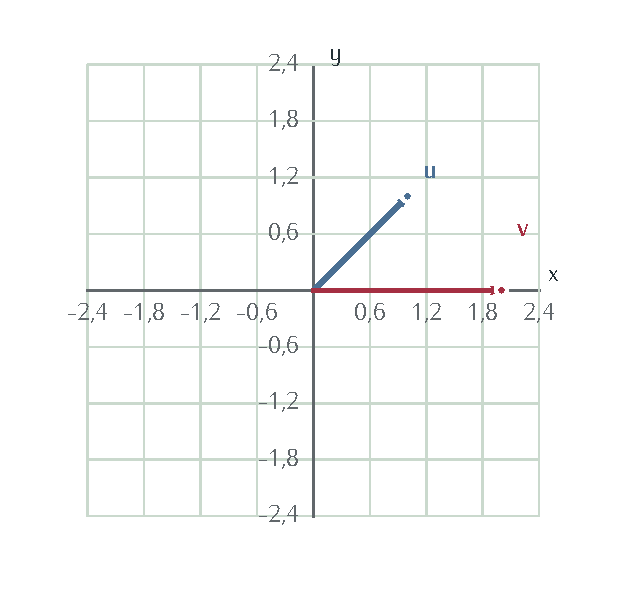
\includegraphics[width=\linewidth,height=94mm,keepaspectratio]{figure/f6be0db70baa6fef6.pdf}\FigureCaption{2.05 \(\cdot\) esempio 1 \(\cdot\) Vettori reali con angolo \(45{}^{\circ} \)}\end{FigureBlock}

\phantomsection\label{c2-prodotto-interno-example-1-step-1}
\BookHeading{01 Coniugare il primo argomento}

\MathBlock{0075002A0020003D002000280031002C002000310029}{u{}^{*}\ =\ (1,\allowbreak \ 1)}
\MathBlock{27E80075002C007627E9003D00280031002900B70028003200290020002B002000280031002900B7002800300029003D0032}{\langle u,\allowbreak v\rangle =(1)\cdot (2)\ +\ (1)\cdot (0)=2}

Il coniugio precede la moltiplicazione componente per componente.\par


\phantomsection\label{c2-prodotto-interno-example-1-step-2}
\BookHeading{02 Controllare lo scambio}

\MathBlock{27E80076002C007527E9003D00280032002900B70028003100290020002B002000280030002900B7002800310029003D0032003D27E80075002C007627E9002A}{\langle v,\allowbreak u\rangle =(2)\cdot (1)\ +\ (0)\cdot (1)=2=\langle u,\allowbreak v\rangle {}^{*}}

Scambiare gli argomenti coniuga il risultato.\par


\phantomsection\label{c2-prodotto-interno-example-1-step-3}
\BookHeading{03 Confrontare prodotto e norme}

\MathBlock{27E80075002C007527E9003D00280031002900B70028003100290020002B002000280031002900B7002800310029003D0032}{\langle u,\allowbreak u\rangle =(1)\cdot (1)\ +\ (1)\cdot (1)=2}
\MathBlock{27E80076002C007627E9003D00280032002900B70028003200290020002B002000280030002900B7002800300029003D0034}{\langle v,\allowbreak v\rangle =(2)\cdot (2)\ +\ (0)\cdot (0)=4}

Le norme quadre sono reali e positive perché ogni fattore è moltiplicato per il proprio coniugato.\par


\phantomsection\label{c2-prodotto-interno-example-1-step-4}
\BookHeading{04 Ricavare l'angolo reale}

\MathBlock{0063006F0073002003B8003D27E80075002C007627E9002F00282016007520162016007620160029003D0032002F0028221A003200B700320029003D0031002F221A0032003B002003B8003D0034003500B0}{\cos \ \theta =\langle u,\allowbreak v\rangle /(\Vert u\Vert \Vert v\Vert )=2/(\sqrt{2}\cdot 2)=1/\sqrt{2};\allowbreak \ \theta =45{}^{\circ} }

Nel piano reale il prodotto interno diviso per le norme determina il coseno dell'angolo.\par


\BookHeading{Interpretazione}

Il prodotto interno vale 2 e l'angolo è \(45{}^{\circ} \). Nella prossima costruzione questo coefficiente permetterà di separare una componente parallela.\par


\Needspace{.36\textheight}\phantomsection\label{c2-prodotto-interno-example-2}
{\sffamily\small\color{Accent} ESEMPIO SVOLTO 2\par}
\BookHeading{Ortogonalità con componenti complesse}
Dati \(u=(1\); \(i)^{T}\), \(v=(i\); \(1)^{T}\).\par


\BookHeading{Geometria e configurazione dell'esempio}
\begin{FigureBlock}\begin{minipage}[t]{.485\linewidth}\centering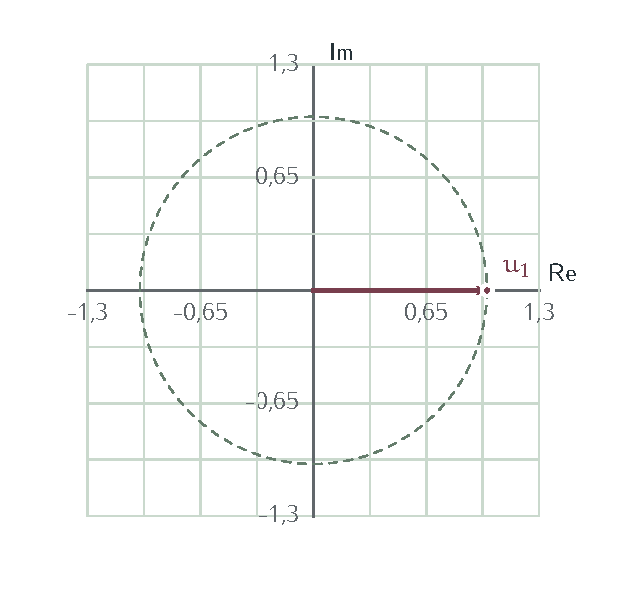
\includegraphics[width=\linewidth,height=63mm,keepaspectratio]{figure/f7ec5472863a9368f.pdf}\par{\sffamily\footnotesize \(u_{1}\)\par}\end{minipage}\hfill\begin{minipage}[t]{.485\linewidth}\centering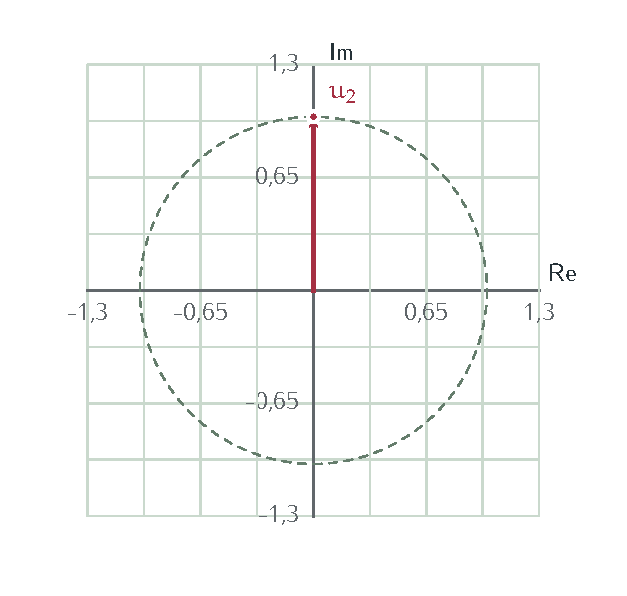
\includegraphics[width=\linewidth,height=63mm,keepaspectratio]{figure/fd6f70e8a1d3861cd.pdf}\par{\sffamily\footnotesize \(u_{2}\)\par}\end{minipage}\FigureCaption{2.05 \(\cdot\) esempio 2 \(\cdot\) Componenti dei due vettori di \(C^{2}\)}\end{FigureBlock}
\begin{FigureBlock}\begin{minipage}[t]{.485\linewidth}\centering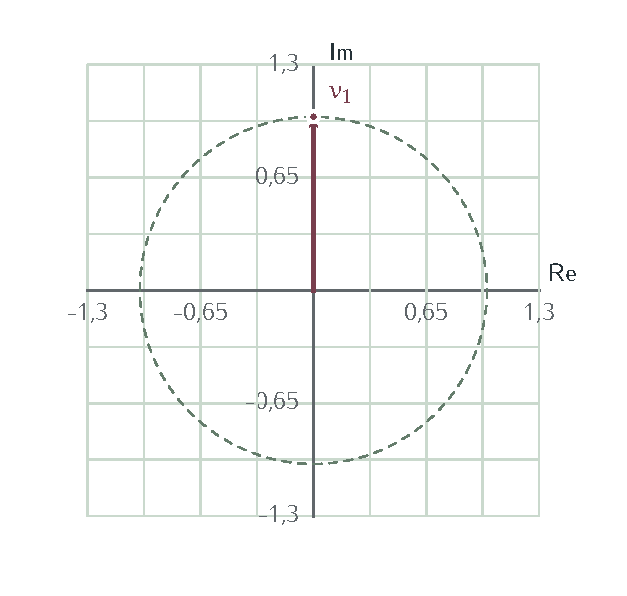
\includegraphics[width=\linewidth,height=63mm,keepaspectratio]{figure/fa34233d9a483bc74.pdf}\par{\sffamily\footnotesize \(v_{1}\)\par}\end{minipage}\hfill\begin{minipage}[t]{.485\linewidth}\centering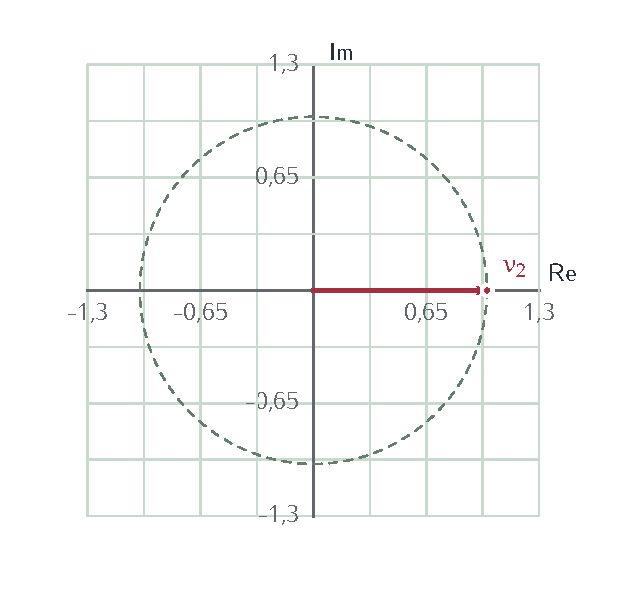
\includegraphics[width=\linewidth,height=63mm,keepaspectratio]{figure/f8cc3952a894de76d.pdf}\par{\sffamily\footnotesize \(v_{2}\)\par}\end{minipage}\FigureCaption{2.05 \(\cdot\) esempio 2 \(\cdot\) Componenti dei due vettori di \(C^{2}\)}\end{FigureBlock}

\phantomsection\label{c2-prodotto-interno-example-2-step-1}
\BookHeading{01 Coniugare il primo argomento}

\MathBlock{0075002A0020003D002000280031002C0020221200690029}{u{}^{*}\ =\ (1,\allowbreak \ - i)}
\MathBlock{27E80075002C007627E9003D00280031002900B70028006900290020002B0020002822120069002900B7002800310029003D0030}{\langle u,\allowbreak v\rangle =(1)\cdot (i)\ +\ (- i)\cdot (1)=0}

Il coniugio precede la moltiplicazione componente per componente.\par


\phantomsection\label{c2-prodotto-interno-example-2-step-2}
\BookHeading{02 Controllare lo scambio}

\MathBlock{27E80076002C007527E9003D002822120069002900B70028003100290020002B002000280031002900B7002800690029003D0030003D27E80075002C007627E9002A}{\langle v,\allowbreak u\rangle =(- i)\cdot (1)\ +\ (1)\cdot (i)=0=\langle u,\allowbreak v\rangle {}^{*}}

Scambiare gli argomenti coniuga il risultato.\par


\phantomsection\label{c2-prodotto-interno-example-2-step-3}
\BookHeading{03 Confrontare prodotto e norme}

\MathBlock{27E80075002C007527E9003D00280031002900B70028003100290020002B0020002822120069002900B7002800690029003D0032}{\langle u,\allowbreak u\rangle =(1)\cdot (1)\ +\ (- i)\cdot (i)=2}
\MathBlock{27E80076002C007627E9003D002822120069002900B70028006900290020002B002000280031002900B7002800310029003D0032}{\langle v,\allowbreak v\rangle =(- i)\cdot (i)\ +\ (1)\cdot (1)=2}

Le norme quadre sono reali e positive perché ogni fattore è moltiplicato per il proprio coniugato.\par


\phantomsection\label{c2-prodotto-interno-example-2-step-4}
\BookHeading{04 Verificare l'ortogonalità complessa}

\MathBlock{27E80075002C007627E9003D003100B70069002B002822120069002900B70031003D006922120069003D0030}{\langle u,\allowbreak v\rangle =1\cdot i+(- i)\cdot 1=i- i=0}

L'ortogonalità riguarda i vettori di \(C^{2}\); i piani delle singole componenti mostrano soltanto gli elementi del calcolo.\par


\BookHeading{Interpretazione}

Il prodotto interno si annulla per cancellazione fra i e \(- i\). La normalizzazione dei due vettori conserva questa ortogonalità.\par


\Needspace{7\baselineskip}
\BookHeading{Il passaggio successivo}
Il coefficiente ottenuto dal prodotto interno permette di sottrarre una componente parallela; applicheremo questa idea per costruire una base ortonormale.\par


% Authoritative exercise source. Preserve all derivations and diagrams.

\ExerciseStart{G2.04}{Calcolare prodotti interni e proiezioni}{Guida esplicita}

\BookHeading{Problema, dati e obiettivo}

Siano \(u=(1,i)^T/\sqrt2\) e \(v=(2,1)^T\). Calcolare la proiezione p di v sulla direzione u e il residuo w. Verificare ortogonalità e identità di Pitagora nel prodotto interno complesso.

\ExTheory{\ExRef{c2-prodotto-interno}{2.05}}{Per u unitario, \(p=u\langle u|v\rangle\), \(w=v-p\). Il primo argomento del prodotto interno va coniugato. La relazione \(\langle u|w\rangle=0\) esprime ortogonalità nello spazio complesso.}

\ExPrediction{Il coefficiente di proiezione sarà complesso perché u contiene i. La decomposizione finale separerà due vettori ortogonali; le loro norme potranno essere rappresentate come cateti di un triangolo reale.}

\ExFigure{\begin{tikzpicture}[>=Stealth,exlabel]
\draw[exaxis] (-0.35,0)--(1.55,0) node[right] {$\operatorname{Re}$};\draw[exaxis] (0,-0.35)--(0,1.55) node[above] {$\operatorname{Im}$};\draw[->,Secondary,line width=1.1pt] (0,0)--(1,0) node[anchor=south west] {$ 1 $};\draw[->,Accent,line width=1.1pt] (0,0)--(0,1) node[anchor=south west] {$ i $};
\end{tikzpicture}}{Le componenti non normalizzate di u sono 1 e i; il bra contiene il coniugato \(-i\).}


\begin{ExTasks}

\item Controllare la norma di u e costruire il bra.

\item Svolgere il prodotto interno.

\item Moltiplicare il coefficiente per entrambe le componenti di u.

\item Sottrarre la proiezione da v e verificare l’ortogonalità.

\item Calcolare le tre norme al quadrato e confrontarle.

\end{ExTasks}

\ExSolution

\ExStep{Preparare il prodotto interno}

\ExEq{u^\dagger&=(1,-i)/\sqrt2,\qquad u^\dagger u=(1+(-i)i)/2=1.}

\ExStep{Calcolare il coefficiente}

\ExEq{c=\langle u|v\rangle&=\frac{1\cdot2+(-i)\cdot1}{\sqrt2}
=\frac{2-i}{\sqrt2}.}
Il coniugio determina il segno della parte immaginaria.

\ExStep{Costruire la proiezione}

\ExEq{p=cu&=\frac12\colv{2-i\\i(2-i)}
=\frac12\colv{2-i\\1+2i}
=\colv{1-i/2\\1/2+i}.}
Nel secondo elemento si è usato \(i(2-i)=2i-i^2=1+2i\).

\ExStep{Calcolare e verificare il residuo}

\ExEq{w&=\colv{2-(1-i/2)\\1-(1/2+i)}=\colv{1+i/2\\1/2-i},\\\langle u|w\rangle&=\frac{1+i/2-i(1/2-i)}{\sqrt2}
=\frac{1+i/2-i/2-1}{\sqrt2}=0.}

\ExStep{Confrontare le norme}

\ExEq{\|p\|^2&=1+1/4+1/4+1=5/2,\\\|w\|^2&=1+1/4+1/4+1=5/2,\\\|v\|^2&=2^2+1^2=5=5/2+5/2.}
Inoltre \(p+w=(2,1)^T\). I due controlli verificano sia la ricostruzione sia l’ortogonalità.

\par\noindent\begin{minipage}{\linewidth}
\ExFigure{\begin{tikzpicture}[>=Stealth,exlabel]
\draw[exaxis] (-0.35,0)--(2.1311400000000003,0) node[right] {$\widehat p$};\draw[exaxis] (0,-0.35)--(0,2.1311400000000003) node[above] {$\widehat w$};\draw[->,Secondary,line width=1.1pt] (0,0)--(1.58114,0) node[anchor=south west] {$ p $};\draw[->,Ink,line width=1.1pt] (0,0)--(0,1.58114) node[anchor=south west] {$ w $};\draw[->,Accent,line width=1.1pt] (0,0)--(1.58114,1.58114) node[anchor=south west] {$ v $};
\end{tikzpicture}}{Piano reale generato da \(p/\|p\|\) e \(w/\|w\|\) all’interno di \(\mathbb C^2\). Le coordinate di v sono le due norme \(\sqrt{5/2}\).}


\ExInterpret{La perpendicolarità riguarda i vettori completi e il prodotto interno dichiarato. Le frecce che mostrano singole componenti nel piano complesso hanno un significato differente dal triangolo delle due parti ortogonali.}

\ExLab{Nella sezione 2.05 confrontare il ruolo del coniugio nei prodotti interni degli esempi. Ricostruire i valori p e w nei piani delle componenti; verificare che omettere il coniugio nel coefficiente impedisca il controllo di ortogonalità.}


\end{minipage}

\Needspace{.43\textheight}
\section{Costruire direzioni ortonormali}
\phantomsection\label{c2-proiezioni}

{\sffamily\small\color{Ink!70} Riferimento alle slide: p. 45.\par}

{\sffamily\small\color{Ink!70} Laboratorio locale: \nolinkurl{index.html#capitolo-2/proiezioni}\par}

\BookHeading{Definizioni e costruzione}
Sottraendo la proiezione lungo una direzione già nota otteniamo il residuo ortogonale. Questa costruzione conduce a Gram--Schmidt.\par

Si costruisce dapprima un asse unitario e si calcola il contributo del vettore successivo lungo quell'asse. Sottraendo tale contributo si ottiene un residuo w con prodotto interno nullo rispetto al primo asse: la sottrazione ha eliminato precisamente la parte parallela.\par

Se il residuo è non nullo, la sua normalizzazione fornisce un secondo asse unitario. Se è nullo, il vettore aggiunto appartiene già allo spazio generato dal primo. La stessa procedura può proseguire in dimensioni maggiori sottraendo tutte le proiezioni già disponibili.\par


\MathBlock{00652081003D0075002F201600752016003B002003B1003D27E800652081002C007627E9003B00200077003D0076221203B100652081003B002000652082003D0077002F201600772016002E}{e_{1}=u/\Vert u\Vert ;\allowbreak \ \alpha =\langle e_{1},\allowbreak v\rangle ;\allowbreak \ w=v- \alpha e_{1};\allowbreak \ e_{2}=w/\Vert w\Vert .}

\BookHeading{Come leggere le figure}
Piano reale con proiezione parallela e residuo ortogonale.\par


\Needspace{.36\textheight}\phantomsection\label{c2-proiezioni-example-1}
{\sffamily\small\color{Accent} ESEMPIO SVOLTO 1\par}
\BookHeading{Due assi ottenuti per sottrazione}
Dati \(u=(1{,}1)\), \(v=(2\); \(0)^{T}\).\par


\BookHeading{Geometria e configurazione dell'esempio}
\begin{FigureBlock}\centering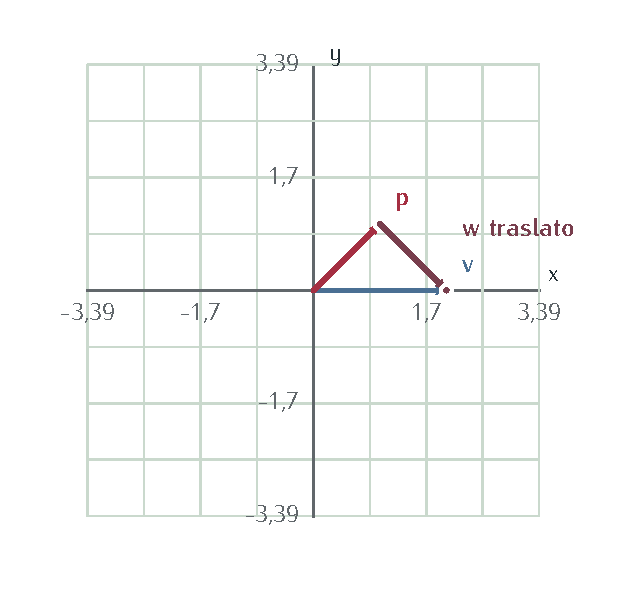
\includegraphics[width=\linewidth,height=94mm,keepaspectratio]{figure/fdfc0e18d3c6c0cf9.pdf}\FigureCaption{2.06 \(\cdot\) esempio 1 \(\cdot\) Proiezione e residuo, stessa scala}\end{FigureBlock}

\phantomsection\label{c2-proiezioni-example-1-step-1}
\BookHeading{01 Costruire il primo asse}

\MathBlock{20160075201600B2003D003100B2002B003100B2003D0032003B002000652081003D00280031002C00310029002F221A0032}{\Vert u\Vert ^{2}=1^{2}+1^{2}=2;\allowbreak \ e_{1}=(1{,}1)/\sqrt{2}}

La norma non nulla permette di ottenere una direzione unitaria.\par


\phantomsection\label{c2-proiezioni-example-1-step-2}
\BookHeading{02 Separare la parte parallela}

\MathBlock{03B1003D27E800652081002C007627E9003D00280032002B00300029002F221A0032}{\alpha =\langle e_{1},\allowbreak v\rangle =(2+0)/\sqrt{2}}
\MathBlock{0070003D03B100652081003D00280031002C00310029}{p=\alpha e_{1}=(1{,}1)}

Il coefficiente è il prodotto interno; moltiplicarlo per \(e_{1}\) ricostruisce il vettore parallelo.\par


\phantomsection\label{c2-proiezioni-example-1-step-3}
\BookHeading{03 Sottrarre il residuo}

\MathBlock{0077003D007622120070003D00280031002C221200310029003B002027E800652081002C007727E9003D00280031221200310029002F221A0032003D0030}{w=v- p=(1,\allowbreak - 1);\allowbreak \ \langle e_{1},\allowbreak w\rangle =(1- 1)/\sqrt{2}=0}

La sottrazione elimina il contributo nella prima direzione.\par


\phantomsection\label{c2-proiezioni-example-1-step-4}
\BookHeading{04 Normalizzare il secondo asse}

\MathBlock{20160077201600B2003D003100B2002B002822120031002900B2003D0032003B002000652082003D00280031002C221200310029002F221A0032003B002027E800652081002C0065208227E9003D0030}{\Vert w\Vert ^{2}=1^{2}+(- 1)^{2}=2;\allowbreak \ e_{2}=(1,\allowbreak - 1)/\sqrt{2};\allowbreak \ \langle e_{1},\allowbreak e_{2}\rangle =0}

I due assi hanno norma uno e prodotto interno nullo, quindi costituiscono una base ortonormale.\par


\BookHeading{Interpretazione}

La somma \((1{,}1)+(1,\allowbreak - 1)\) ricostruisce (2,0); la seconda direzione nasce dal residuo ortogonale.\par


\Needspace{.36\textheight}\phantomsection\label{c2-proiezioni-example-2}
{\sffamily\small\color{Accent} ESEMPIO SVOLTO 2\par}
\BookHeading{Residuo nullo e vettori dipendenti}
Dati \(u=(1{,}1)\), \(v=(2\); \(2)^{T}\).\par


\BookHeading{Geometria e configurazione dell'esempio}
\begin{FigureBlock}\centering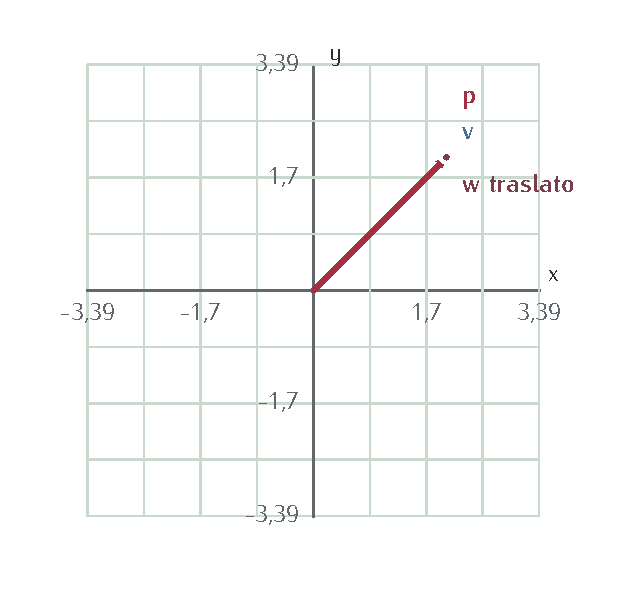
\includegraphics[width=\linewidth,height=94mm,keepaspectratio]{figure/f62440d0188b16f01.pdf}\FigureCaption{2.06 \(\cdot\) esempio 2 \(\cdot\) Proiezione e residuo, stessa scala}\end{FigureBlock}

\phantomsection\label{c2-proiezioni-example-2-step-1}
\BookHeading{01 Costruire il primo asse}

\MathBlock{20160075201600B2003D003100B2002B003100B2003D0032003B002000652081003D00280031002C00310029002F221A0032}{\Vert u\Vert ^{2}=1^{2}+1^{2}=2;\allowbreak \ e_{1}=(1{,}1)/\sqrt{2}}

La norma non nulla permette di ottenere una direzione unitaria.\par


\phantomsection\label{c2-proiezioni-example-2-step-2}
\BookHeading{02 Separare la parte parallela}

\MathBlock{03B1003D27E800652081002C007627E9003D00280032002B00320029002F221A0032}{\alpha =\langle e_{1},\allowbreak v\rangle =(2+2)/\sqrt{2}}
\MathBlock{0070003D03B100652081003D00280032002C00320029}{p=\alpha e_{1}=(2{,}2)}

Il coefficiente è il prodotto interno; moltiplicarlo per \(e_{1}\) ricostruisce il vettore parallelo.\par


\phantomsection\label{c2-proiezioni-example-2-step-3}
\BookHeading{03 Sottrarre il residuo}

\MathBlock{0077003D007622120070003D00280030002C00300029003B002027E800652081002C007727E9003D0030}{w=v- p=(0{,}0);\allowbreak \ \langle e_{1},\allowbreak w\rangle =0}

La sottrazione elimina il contributo nella prima direzione.\par


\phantomsection\label{c2-proiezioni-example-2-step-4}
\BookHeading{04 Riconoscere la dipendenza}

\MathBlock{20160077201600B2003D0030003B00200076003D00320075003B0020006E0065007300730075006E002000652082003D0077002F201600772016002000E800200064006500660069006E00690074006F}{\Vert w\Vert ^{2}=0;\allowbreak \ v=2u;\allowbreak \ \text{nessun}\ e_{2}=w/\Vert w\Vert \ \text{è}\ \text{definito}}

Un residuo nullo non aggiunge una nuova direzione. La procedura si ferma con un solo asse.\par


\BookHeading{Interpretazione}

La proiezione coincide con v e il residuo è esattamente nullo. La normalizzazione del residuo sarebbe una divisione per zero.\par


\Needspace{7\baselineskip}
\BookHeading{Il passaggio successivo}
Le proiezioni hanno mostrato come costruire direzioni utili. Descriveremo ora una trasformazione indicando dove manda i vettori di una base.\par


% Authoritative exercise source. Preserve all derivations and diagrams.

\ExerciseStart{G2.05}{Costruire una base con Gram–Schmidt}{Guida esplicita}

\BookHeading{Problema, dati e obiettivo}

Nello spazio reale \(\mathbb R^2\), con prodotto interno euclideo, siano \(u=(1,1)^T\) e \(v=(2,0)^T\). Costruire una base ortonormale mediante Gram--Schmidt, ricostruire \(v\) nella nuova base e discutere che cosa accadrebbe sostituendo \(v\) con \(v^{\prime}=3u\).

\ExTheory{\ExRef{c2-proiezioni}{2.06}}{La norma è \(\|u\|=\sqrt{\inner{u}{u}}\). Data una direzione unitaria \(e_1\), la proiezione di \(v\) è \(p=e_1\inner{e_1}{v}\). Il residuo \(w=v-p\) è ortogonale a \(e_1\). Se \(w\ne0\), \(e_2=w/\|w\|\) completa la base.}

\ExPrediction{Tracciare la diagonale individuata da \(u\). La proiezione di \(v\) deve appartenere a tale retta; il segmento che unisce la proiezione a \(v\) deve esserle perpendicolare. Prevedere il segno della seconda componente del residuo.}

\ExFigure{\begin{tikzpicture}[>=Stealth,exlabel]
\draw[exaxis] (-0.35,0)--(2.55,0) node[right] {$x_1$};\draw[exaxis] (0,-0.35)--(0,1.55) node[above] {$x_2$};\draw[->,Secondary,line width=1.1pt] (0,0)--(1,1) node[anchor=south west] {$ u $};\draw[->,Accent,line width=1.1pt] (0,0)--(2,0) node[anchor=south west] {$ v $};
\end{tikzpicture}}{Piano delle coordinate reali. Le lunghezze e gli angoli sono quelli del prodotto interno euclideo.}


\begin{ExTasks}

\item Calcolare \(\inner{u}{u}\) e normalizzare \(u\).

\item Eseguire il prodotto interno \(\inner{e_1}{v}\) e costruire \(p\).

\item Sottrarre \(p\) da \(v\), componente per componente.

\item Normalizzare il residuo e verificare i tre prodotti interni della base.

\item Calcolare le coordinate di \(v\) nella base ottenuta e ricostruirlo.

\item Ripetere la sottrazione per \(v^{\prime}=3u\) e spiegare il residuo nullo.

\end{ExTasks}

\ExSolution

\ExStep{Normalizzare la prima direzione}

Si ottiene
\ExEq{\inner{u}{u}&=1\cdot1+1\cdot1=2,\quad\|u\|=\sqrt2,\\e_1&=\frac1{\sqrt2}\colv{1\\1}.}
Le coordinate cambiano di un fattore comune; la retta generata dal vettore rimane la stessa.

\ExStep{Calcolare la proiezione}

Il coefficiente lungo \(e_1\) è uno scalare:
\ExEq{\inner{e_1}{v}&=\frac1{\sqrt2}\cdot2+\frac1{\sqrt2}\cdot0
=\frac2{\sqrt2}=\sqrt2,\\p&=\sqrt2\,e_1=\frac{\sqrt2}{\sqrt2}\colv{1\\1}=\colv{1\\1}.}
La proiezione è il vettore \(p\); il numero \(\sqrt2\) ne misura la componente nella direzione unitaria.

\ExStep{Isolare e normalizzare il residuo}

Si sottraggono le componenti:
\ExEq{w&=v-p=\colv{2-1\\0-1}=\colv{1\\-1},\\
\|w\|^2&=1^2+(-1)^2=2,\qquad e_2=\frac1{\sqrt2}\colv{1\\-1}.}
Il segno negativo della seconda coordinata porta dal punto \((1,1)\) al punto \((2,0)\).

\ExStep{Verificare l’ortonormalità}

I controlli sono distinti:
\ExEq{\inner{e_1}{e_1}&=\tfrac12+\tfrac12=1,\\
\inner{e_2}{e_2}&=\tfrac12+\tfrac12=1,\\
\inner{e_1}{e_2}&=\tfrac12-\tfrac12=0.}
La matrice \(E=(e_1\ e_2)\) soddisfa quindi \(E^TE=I\).

\ExStep{Ricostruire il vettore}

La seconda coordinata vale \(\inner{e_2}{v}=2/\sqrt2+0=\sqrt2\). Pertanto
\ExEq{[v]_E&=\colv{\sqrt2\\\sqrt2},\\
E[v]_E&=\frac1{\sqrt2}\begin{pmatrix}1&1\\1&-1\end{pmatrix}\colv{\sqrt2\\\sqrt2}
=\colv{(\sqrt2+\sqrt2)/\sqrt2\\(\sqrt2-\sqrt2)/\sqrt2}=\colv{2\\0}.}
Anche la norma si conserva: \(2^2+0^2=4\) e \((\sqrt2)^2+(\sqrt2)^2=4\).

\ExStep{Riconoscere la dipendenza}

Per \(v'=(3,3)^T\), il coefficiente è \(3/\sqrt2+3/\sqrt2=3\sqrt2\). Quindi
\ExEq{p'&=3\sqrt2\,e_1=\colv{3\\3},\qquad w'=v'-p'=\colv{0\\0}.}
La norma nulla impedisce la divisione. I due vettori descrivono una sola direzione: per una base del piano occorrerebbe scegliere un secondo vettore indipendente.

\par\noindent\begin{minipage}{\linewidth}
\ExFigure{\begin{tikzpicture}[>=Stealth,exlabel]
\draw[exaxis] (-0.35,0)--(2.55,0) node[right] {$x_1$};\draw[exaxis] (0,-1.35)--(0,1.55) node[above] {$x_2$};\draw[->,Secondary,line width=1.1pt] (0,0)--(1,1) node[anchor=south west] {$ p $};\draw[->,Accent,line width=1.1pt] (0,0)--(2,0) node[anchor=south west] {$ v $};\draw[->,Ink,line width=1.1pt] (0,0)--(1,-1) node[anchor=north west] {$ w $};\draw[Secondary,dashed,->] (1,1)--(2,0);\draw[Ink!30,dashed] (-1.6,-1.6)--(2,2);
\end{tikzpicture}}{La decomposizione è \(v=p+w\). Il residuo disegnato dall’origine è parallelo al segmento tratteggiato.}


\ExInterpret{La proiezione separa la componente lungo la prima direzione; la sottrazione conserva la parte necessaria a generare la seconda. In uno spazio complesso il primo argomento del prodotto interno sarebbe coniugato. Il residuo nullo segnala una dipendenza dei dati.}

\ExLab{Aprire lo strumento di esplorazione della sezione 2.06. Inserire \(u_1=1,u_2=1,v_1=2,v_2=0\) e confrontare proiezione e residuo con la figura. Sostituire poi \(v_1=v_2=3\): verificare che non venga costruita una seconda direzione normalizzata dal vettore nullo.}


\end{minipage}

\Needspace{.43\textheight}
\section{La matrice attraverso le sue colonne}
\phantomsection\label{c2-matrici}

{\sffamily\small\color{Ink!70} Riferimento alle slide: p. 76.\par}

{\sffamily\small\color{Ink!70} Laboratorio locale: \nolinkurl{index.html#capitolo-2/matrici}\par}

\BookHeading{Definizioni e costruzione}
Una trasformazione lineare è determinata dall'immagine dei vettori della base. Il prodotto riga per colonna ricostruisce la stessa trasformazione.\par

La linearità richiede \(A(\alpha u+\beta v)=\alpha Au+\beta Av\). Scrivendo un vettore come combinazione dei vettori canonici, questa proprietà mostra che bastano le immagini della base per determinare ogni risultato. Tali immagini compaiono nelle colonne della matrice.\par

Il prodotto riga per colonna e la combinazione delle colonne sono due letture dello stesso calcolo. La figura confronta ingresso e uscita sulla stessa scala, così che una variazione della lunghezza o dell'angolo rimanga riconoscibile. Una trasformazione lineare manda sempre l'origine nell'origine.\par


\MathBlock{00410076003D00762081004100652081002B00762082004100652082002E}{Av=v_{1}Ae_{1}+v_{2}Ae_{2}.}

\BookHeading{Come leggere le figure}
Piano reale: la figura confronta il vettore e la sua immagine sulla medesima scala.\par


\Needspace{.36\textheight}\phantomsection\label{c2-matrici-example-1}
{\sffamily\small\color{Accent} ESEMPIO SVOLTO 1\par}
\BookHeading{Deformazione di taglio}
Dati \(A=\)\(\begin{pmatrix}1&1\\0&1\end{pmatrix}\), \(v=(1\); \(2)^{T}\).\par


\BookHeading{Geometria e configurazione dell'esempio}
\begin{FigureBlock}\centering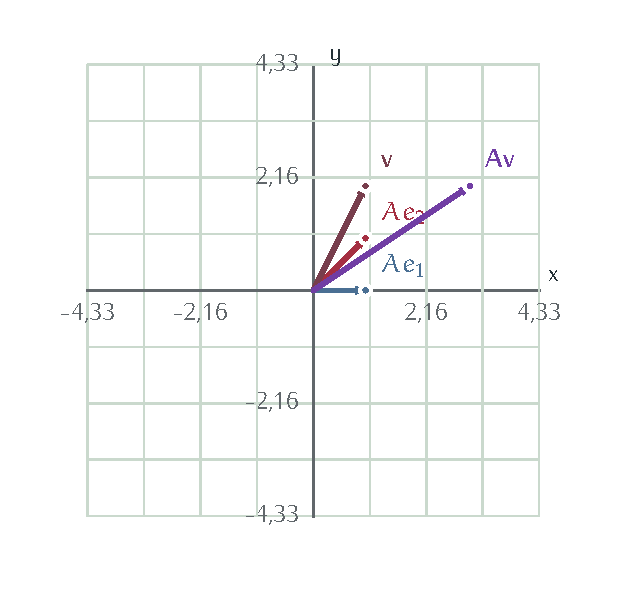
\includegraphics[width=\linewidth,height=94mm,keepaspectratio]{figure/fbb475d8f89ee22b7.pdf}\FigureCaption{2.07 \(\cdot\) esempio 1 \(\cdot\) Colonne, ingresso e immagine}\end{FigureBlock}

\phantomsection\label{c2-matrici-example-1-step-1}
\BookHeading{01 Leggere le colonne}

\MathBlock{004100652081003D00280031003B0020003000291D40003B0020004100652082003D00280031003B0020003100291D40}{Ae_{1}=(1;\allowbreak \ 0)^{T};\allowbreak \ Ae_{2}=(1;\allowbreak \ 1)^{T}}

Le colonne sono le immagini dei due assi canonici e determinano la trasformazione.\par


\phantomsection\label{c2-matrici-example-1-step-2}
\BookHeading{02 Calcolare Av, componente 1}

\MathBlock{00280031002900B70028003100290020002B002000280031002900B7002800320029003D0033}{(1)\cdot (1)\ +\ (1)\cdot (2)=3}

Ogni riga viene moltiplicata per la colonna delle coordinate di v.\par


\phantomsection\label{c2-matrici-example-1-step-3}
\BookHeading{03 Calcolare Av, componente 2}

\MathBlock{00280030002900B70028003100290020002B002000280031002900B7002800320029003D0032}{(0)\cdot (1)\ +\ (1)\cdot (2)=2}

Ogni riga viene moltiplicata per la colonna delle coordinate di v.\par


\phantomsection\label{c2-matrici-example-1-step-4}
\BookHeading{04 Verificare con le colonne}

\MathBlock{00410076003D0031004100652081002B002800320029004100652082003D00280033003B0020003200291D40}{Av=1Ae_{1}+(2)Ae_{2}=(3;\allowbreak \ 2)^{T}}

La combinazione delle immagini degli assi restituisce il prodotto per righe.\par


\BookHeading{Interpretazione}

La seconda colonna è inclinata; la componente verticale resta invariata e quella orizzontale riceve il contributo verticale.\par


\Needspace{.36\textheight}\phantomsection\label{c2-matrici-example-2}
{\sffamily\small\color{Accent} ESEMPIO SVOLTO 2\par}
\BookHeading{Rotazione e dilatazione}
Dati \(A=\)\(\begin{pmatrix}1&-1\\1&1\end{pmatrix}\), \(v=(2\); \(-1)^{T}\).\par


\BookHeading{Geometria e configurazione dell'esempio}
\begin{FigureBlock}\centering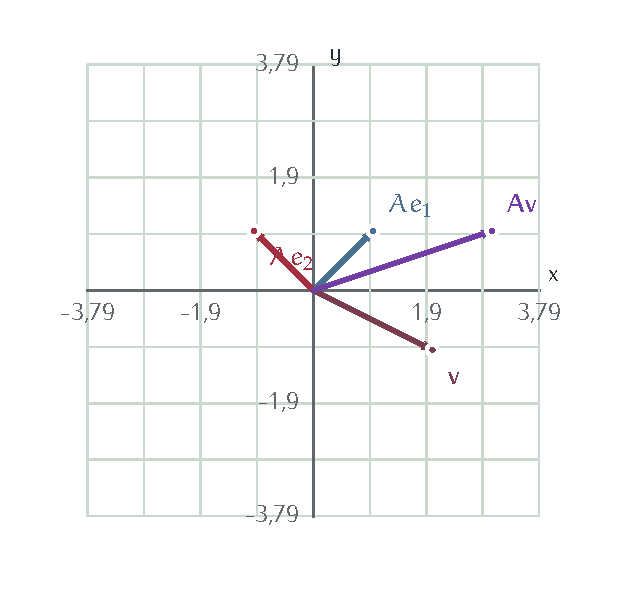
\includegraphics[width=\linewidth,height=94mm,keepaspectratio]{figure/f03a6de58513faf77.pdf}\FigureCaption{2.07 \(\cdot\) esempio 2 \(\cdot\) Colonne, ingresso e immagine}\end{FigureBlock}

\phantomsection\label{c2-matrici-example-2-step-1}
\BookHeading{01 Leggere le colonne}

\MathBlock{004100652081003D00280031003B0020003100291D40003B0020004100652082003D0028002D0031003B0020003100291D40}{Ae_{1}=(1;\allowbreak \ 1)^{T};\allowbreak \ Ae_{2}=(-1;\allowbreak \ 1)^{T}}

Le colonne sono le immagini dei due assi canonici e determinano la trasformazione.\par


\phantomsection\label{c2-matrici-example-2-step-2}
\BookHeading{02 Calcolare Av, componente 1}

\MathBlock{00280031002900B70028003200290020002B00200028002D0031002900B70028002D00310029003D0033}{(1)\cdot (2)\ +\ (-1)\cdot (-1)=3}

Ogni riga viene moltiplicata per la colonna delle coordinate di v.\par


\phantomsection\label{c2-matrici-example-2-step-3}
\BookHeading{03 Calcolare Av, componente 2}

\MathBlock{00280031002900B70028003200290020002B002000280031002900B70028002D00310029003D0031}{(1)\cdot (2)\ +\ (1)\cdot (-1)=1}

Ogni riga viene moltiplicata per la colonna delle coordinate di v.\par


\phantomsection\label{c2-matrici-example-2-step-4}
\BookHeading{04 Verificare con le colonne}

\MathBlock{00410076003D0032004100652081002B0028002D00310029004100652082003D00280033003B0020003100291D40}{Av=2Ae_{1}+(-1)Ae_{2}=(3;\allowbreak \ 1)^{T}}

La combinazione delle immagini degli assi restituisce il prodotto per righe.\par


\BookHeading{Interpretazione}

Le colonne sono ortogonali e hanno lunghezza \(\sqrt{2}\): l'operatore ruota di \(45{}^{\circ} \) e dilata ogni lunghezza di \(\sqrt{2}\).\par


\Needspace{7\baselineskip}
\BookHeading{Il passaggio successivo}
Le colonne determinano tutte le uscite. Studiare quali loro combinazioni si annullano permetterà di identificare nucleo e perdita di informazione.\par


\Needspace{.43\textheight}
\section{Informazione perduta: nucleo e immagine}
\phantomsection\label{c2-nucleo}

{\sffamily\small\color{Ink!70} Riferimento alle slide: p. 160.\par}

{\sffamily\small\color{Ink!70} Laboratorio locale: \nolinkurl{index.html#capitolo-2/nucleo}\par}

\BookHeading{Definizioni e costruzione}
Quando due direzioni vengono mandate sulla stessa retta, alcune differenze fra ingressi scompaiono. Il nucleo raccoglie precisamente queste differenze.\par

Due ingressi u e v hanno la stessa immagine quando \(A(u- v)=0\). Il nucleo contiene quindi le differenze che la trasformazione rende indistinguibili. Per determinarlo si risolve il sistema omogeneo \(Ax=0\), esprimendo le variabili pivot attraverso quelle libere.\par

L'immagine è generata dalle colonne della matrice. Le colonne indipendenti ne determinano la dimensione, chiamata rango. Nel piano, una matrice di rango uno produce risultati su una retta; una matrice nulla produce soltanto l'origine. Il teorema rango-nullità conta insieme direzioni conservate e annullate.\par


\MathBlock{006B0065007200200041003D007B0076003A00410076003D0030007D003B00200069006D00200041003D007B00410076007D003B002000640069006D0020006B0065007200200041002B00720061006E0067006F00200041003D006E0075006D00650072006F00200064006900200063006F006C006F006E006E0065002E}{\text{ker}\ A=\{v:Av=0\};\allowbreak \ im\ A=\{Av\};\allowbreak \ \text{dim}\ \text{ker}\ A+\text{rango}\ A=\text{numero}\ \text{di}\ \text{colonne}.}

\BookHeading{Come leggere le figure}
Piano reale con una direzione annullata dalla trasformazione.\par


\Needspace{.36\textheight}\phantomsection\label{c2-nucleo-example-1}
{\sffamily\small\color{Accent} ESEMPIO SVOLTO 1\par}
\BookHeading{Una direzione cancellata}
Dati \(A=\)\(\begin{pmatrix}1&2\\0&0\end{pmatrix}\), \(v=(1\); \(2)^{T}\).\par


\BookHeading{Geometria e configurazione dell'esempio}
\begin{FigureBlock}\centering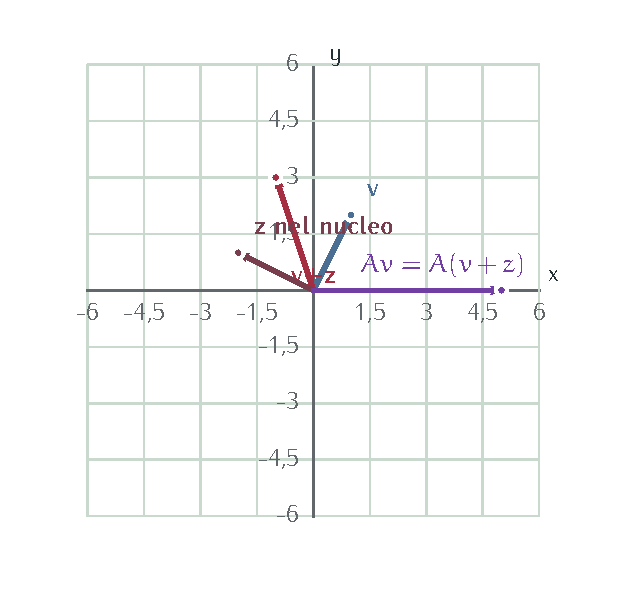
\includegraphics[width=\linewidth,height=94mm,keepaspectratio]{figure/fdef3d88a46f13189.pdf}\FigureCaption{2.08 \(\cdot\) esempio 1 \(\cdot\) Ingressi distinti e immagine comune}\end{FigureBlock}

\phantomsection\label{c2-nucleo-example-1-step-1}
\BookHeading{01 Leggere le colonne}

\MathBlock{004100652081003D00280031003B0020003000291D40003B0020004100652082003D00280032003B0020003000291D40}{Ae_{1}=(1;\allowbreak \ 0)^{T};\allowbreak \ Ae_{2}=(2;\allowbreak \ 0)^{T}}

Le colonne sono le immagini dei due assi canonici e determinano la trasformazione.\par


\phantomsection\label{c2-nucleo-example-1-step-2}
\BookHeading{02 Calcolare Av, componente 1}

\MathBlock{00280031002900B70028003100290020002B002000280032002900B7002800320029003D0035}{(1)\cdot (1)\ +\ (2)\cdot (2)=5}

Ogni riga viene moltiplicata per la colonna delle coordinate di v.\par


\phantomsection\label{c2-nucleo-example-1-step-3}
\BookHeading{03 Calcolare Av, componente 2}

\MathBlock{00280030002900B70028003100290020002B002000280030002900B7002800320029003D0030}{(0)\cdot (1)\ +\ (0)\cdot (2)=0}

Ogni riga viene moltiplicata per la colonna delle coordinate di v.\par


\phantomsection\label{c2-nucleo-example-1-step-4}
\BookHeading{04 Risolvere \(Ax=0\)}

\MathBlock{0078002B00320079003D0030003B00200079003D0074003B00200078003D221200320074003B0020006B0065007200200041003D007B0074002822120032002C00310029007D}{x+2y=0;\allowbreak \ y=t;\allowbreak \ x=- 2t;\allowbreak \ \text{ker}\ A=\{t(- 2{,}1)\}}

Una variabile libera parametrizza una retta di ingressi annullati.\par


\phantomsection\label{c2-nucleo-example-1-step-5}
\BookHeading{05 Descrivere immagine e dimensioni}

\MathBlock{0069006D00200041003D007300700061006E007B00280031002C00300029007D003B002000720061006E0067006F00200041003D0031003B002000640069006D0020006B0065007200200041003D0031003B00200031002B0031003D0032}{im\ A=\text{span}\{(1{,}0)\};\allowbreak \ \text{rango}\ A=1;\allowbreak \ \text{dim}\ \text{ker}\ A=1;\allowbreak \ 1+1=2}

Il rango conta le direzioni indipendenti in uscita; la dimensione del nucleo conta quelle annullate.\par


\phantomsection\label{c2-nucleo-example-1-step-6}
\BookHeading{06 Verificare due ingressi indistinguibili}

\MathBlock{0077003D0076002B007A003D0028002D0031003B0020003300291D40003B00200041007A003D00280030003B0020003000291D40}{w=v+z=(-1;\allowbreak \ 3)^{T};\allowbreak \ Az=(0;\allowbreak \ 0)^{T}}
\MathBlock{00410077003D00280035003B0020003000291D40003D00410076}{Aw=(5;\allowbreak \ 0)^{T}=Av}

Aggiungere un vettore del nucleo lascia invariata l'immagine.\par


\BookHeading{Interpretazione}

Gli ingressi differiscono di \((- 2{,}1)\), che \(A\) annulla. L'uscita è confinata all'asse orizzontale.\par


\Needspace{.36\textheight}\phantomsection\label{c2-nucleo-example-2}
{\sffamily\small\color{Accent} ESEMPIO SVOLTO 2\par}
\BookHeading{Operatore nullo}
Dati \(A=\)\(\begin{pmatrix}0&0\\0&0\end{pmatrix}\), \(v=(2\); \(-1)^{T}\).\par


\BookHeading{Geometria e configurazione dell'esempio}
\begin{FigureBlock}\centering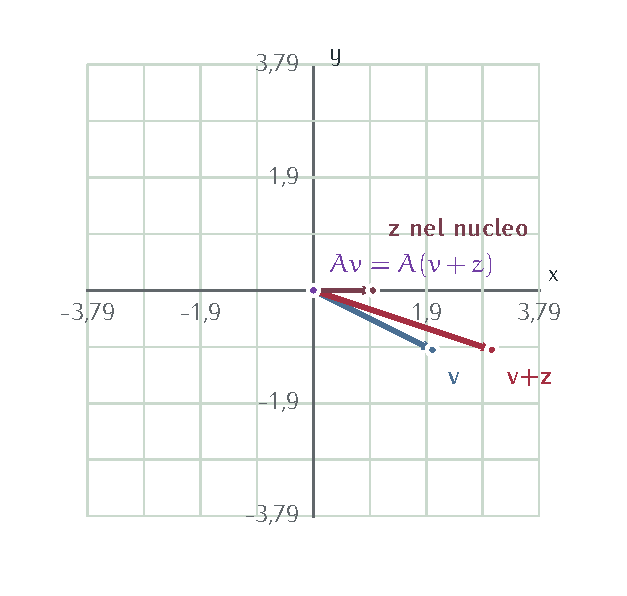
\includegraphics[width=\linewidth,height=94mm,keepaspectratio]{figure/fdbe276dd48572b89.pdf}\FigureCaption{2.08 \(\cdot\) esempio 2 \(\cdot\) Ingressi distinti e immagine comune}\end{FigureBlock}

\phantomsection\label{c2-nucleo-example-2-step-1}
\BookHeading{01 Leggere le colonne}

\MathBlock{004100652081003D00280030003B0020003000291D40003B0020004100652082003D00280030003B0020003000291D40}{Ae_{1}=(0;\allowbreak \ 0)^{T};\allowbreak \ Ae_{2}=(0;\allowbreak \ 0)^{T}}

Le colonne sono le immagini dei due assi canonici e determinano la trasformazione.\par


\phantomsection\label{c2-nucleo-example-2-step-2}
\BookHeading{02 Calcolare Av, componente 1}

\MathBlock{00280030002900B70028003200290020002B002000280030002900B70028002D00310029003D0030}{(0)\cdot (2)\ +\ (0)\cdot (-1)=0}

Ogni riga viene moltiplicata per la colonna delle coordinate di v.\par


\phantomsection\label{c2-nucleo-example-2-step-3}
\BookHeading{03 Calcolare Av, componente 2}

\MathBlock{00280030002900B70028003200290020002B002000280030002900B70028002D00310029003D0030}{(0)\cdot (2)\ +\ (0)\cdot (-1)=0}

Ogni riga viene moltiplicata per la colonna delle coordinate di v.\par


\phantomsection\label{c2-nucleo-example-2-step-4}
\BookHeading{04 Risolvere \(Ax=0\)}

\MathBlock{00300078002B00300079003D0030003B00200078003D0073002C00200079003D0074003B0020006B0065007200200041003D005200B2}{0x+0y=0;\allowbreak \ x=s,\allowbreak \ y=t;\allowbreak \ \text{ker}\ A=R^{2}}

Ogni coppia di coordinate soddisfa il sistema.\par


\phantomsection\label{c2-nucleo-example-2-step-5}
\BookHeading{05 Descrivere immagine e dimensioni}

\MathBlock{0069006D00200041003D007B0030007D003B002000720061006E0067006F00200041003D0030003B002000640069006D0020006B0065007200200041003D0032003B00200030002B0032003D0032}{im\ A=\{0\};\allowbreak \ \text{rango}\ A=0;\allowbreak \ \text{dim}\ \text{ker}\ A=2;\allowbreak \ 0+2=2}

Il rango conta le direzioni indipendenti in uscita; la dimensione del nucleo conta quelle annullate.\par


\phantomsection\label{c2-nucleo-example-2-step-6}
\BookHeading{06 Verificare due ingressi indistinguibili}

\MathBlock{0077003D0076002B007A003D00280033003B0020002D003100291D40003B00200041007A003D00280030003B0020003000291D40}{w=v+z=(3;\allowbreak \ -1)^{T};\allowbreak \ Az=(0;\allowbreak \ 0)^{T}}
\MathBlock{00410077003D00280030003B0020003000291D40003D00410076}{Aw=(0;\allowbreak \ 0)^{T}=Av}

Aggiungere un vettore del nucleo lascia invariata l'immagine.\par


\BookHeading{Interpretazione}

La matrice nulla invia tutto il piano all'origine. Il nucleo ha dimensione due e l'immagine dimensione zero.\par


\Needspace{7\baselineskip}
\BookHeading{Il passaggio successivo}
Dopo aver distinto direzioni conservate e annullate, seguiremo due trasformazioni consecutive per verificare come l'ordine ne cambi l'effetto.\par


% Authoritative exercise source. Preserve all derivations and diagrams.

\ExerciseStart{G2.06}{Leggere una matrice attraverso le immagini della base}{Consolidamento}

\BookHeading{Problema, dati e obiettivo}

Studiare la trasformazione \(A=\begin{pmatrix}1&2\\2&4\end{pmatrix}\). Calcolare le immagini della base canonica, del vettore \(v=(3,-1)^T\) e di \(w=(1,0)^T\); determinare nucleo e immagine.

\ExTheory{\ExRef{c2-matrici}{2.07}; \ExRef{c2-nucleo}{2.08}}{La colonna j di A è l’immagine di \(e_j\). Per \(x=(x_1,x_2)^T\), \(Ax=x_1Ae_1+x_2Ae_2\). Il nucleo contiene i vettori mandati in zero, l’immagine tutti i risultati possibili.}

\ExPrediction{Le colonne sono parallele. Il piano degli ingressi dovrebbe quindi essere mandato su una retta; una direzione intera perderà la propria componente distinguibile.}

\ExFigure{\begin{tikzpicture}[>=Stealth,exlabel]
\draw[exaxis] (-0.35,0)--(1.55,0) node[right] {$x_1$};\draw[exaxis] (0,-0.35)--(0,1.55) node[above] {$x_2$};\draw[->,Accent,line width=1.1pt] (0,0)--(1,0) node[anchor=south west] {$ e_1 $};\draw[->,Secondary,line width=1.1pt] (0,0)--(0,1) node[anchor=south west] {$ e_2 $};
\end{tikzpicture}}{Base del piano di ingresso.}


\begin{ExTasks}

\item Leggere e verificare le due colonne.

\item Eseguire il prodotto con v.

\item Eseguire il prodotto con w e confrontare gli ingressi.

\item Risolvere \(Ax=0\).

\item Parametrizzare l’immagine e spiegare il rango.

\end{ExTasks}

\ExSolution

\ExStep{Applicare A alla base}

\ExEq{Ae_1&=\colv{1\cdot1+2\cdot0\\2\cdot1+4\cdot0}=\colv{1\\2},\\Ae_2&=\colv{1\cdot0+2\cdot1\\2\cdot0+4\cdot1}=\colv{2\\4}=2Ae_1.}

\ExStep{Trasformare il primo ingresso}

\ExEq{Av&=\colv{1\cdot3+2(-1)\\2\cdot3+4(-1)}=\colv{3-2\\6-4}=\colv{1\\2}.}

\ExStep{Confrontare un altro ingresso}

\ExEq{Aw&=\colv{1\cdot1+2\cdot0\\2\cdot1+4\cdot0}=\colv{1\\2}.}
La differenza è \(v-w=(2,-1)^T\). Applicando A si ottiene \((2-2,4-4)^T=(0,0)^T\).

\ExStep{Risolvere il sistema del nucleo}

\ExEq{x_1+2x_2&=0,\qquad2x_1+4x_2=0.}
La seconda equazione è il doppio della prima. Posto \(x_2=t\), si ha \(x_1=-2t\), dunque \(\ker A=\{t(-2,1)^T:t\in\mathbb R\}\).

\ExStep{Ricavare l’immagine}

\ExEq{Ax&=\colv{x_1+2x_2\\2(x_1+2x_2)}=(x_1+2x_2)\colv{1\\2}.}
Ogni multiplo è ottenibile scegliendo \(x_2=0\). L’immagine è \(\operatorname{span}\{(1,2)^T\}\), di dimensione 1. La dimensione del nucleo è 1 e \(1+1=2\) verifica il teorema rango-nullità.

\par\noindent\begin{minipage}{\linewidth}
\ExFigure{\begin{tikzpicture}[>=Stealth,exlabel]
\draw[exaxis] (-0.35,0)--(2.55,0) node[right] {$x_1$};\draw[exaxis] (0,-0.35)--(0,4.55) node[above] {$x_2$};\draw[->,Accent,line width=1.1pt] (0,0)--(1,2) node[anchor=south west] {$ Ae_1 $};\draw[->,Secondary,line width=1.1pt] (0,0)--(2,4) node[anchor=south west] {$ Ae_2 $};
\end{tikzpicture}}{Le immagini delle due direzioni di base appartengono alla medesima retta.}


\ExInterpret{A conserva soltanto la combinazione \(x_1+2x_2\). Il determinante \(1\cdot4-2\cdot2=0\) conferma la perdita di invertibilità. Una trasformazione di questo tipo non rappresenta da sola l’evoluzione unitaria di un sistema quantistico chiuso.}

\ExLab{Nelle sezioni 2.07–2.08 inserire la matrice nello strumento delle trasformazioni e confrontare immagini della base, griglia trasformata e nucleo. Muovere l’ingresso lungo una retta parallela a \((-2,1)\): l’uscita resta invariata.}


\end{minipage}

\Needspace{.43\textheight}
\section{Seguire l'ordine delle operazioni}
\phantomsection\label{c2-composizione}

{\sffamily\small\color{Ink!70} Riferimento alle slide: p. 138.\par}

{\sffamily\small\color{Ink!70} Laboratorio locale: \nolinkurl{index.html#capitolo-2/composizione}\par}

\BookHeading{Definizioni e costruzione}
Il risultato della prima trasformazione diventa l'ingresso della seconda. Scriviamo ogni stato intermedio prima di raccogliere le operazioni in un prodotto.\par

Una composizione viene letta a partire dall'ingresso: se si applica \(B\) e poi \(A\), il primo risultato è Bv e il secondo è A(Bv). La notazione AB raccoglie questa successione mantenendo il fattore che agisce per primo a destra.\par

Il confronto con BA deve usare lo stesso vettore iniziale. Due trasformazioni possono dare risultati diversi quando vengono scambiate; il commutatore \([A,\allowbreak B]=AB- BA\) quantifica questa differenza. Conservare i risultati intermedi permette di riconoscere quale operazione produce ciascun cambiamento.\par


\MathBlock{005000720069006D006100200042002C00200070006F006900200041003A0020007621A60042007621A600410028004200760029003D00280041004200290076002E}{\text{Prima}\ B,\allowbreak \ \text{poi}\ A:\ v\mapsto Bv\mapsto A(Bv)=(AB)v.}

\BookHeading{Come leggere le figure}
Piano reale; le frecce mostrano risultati successivi riferiti alla stessa origine.\par


\Needspace{.36\textheight}\phantomsection\label{c2-composizione-example-1}
{\sffamily\small\color{Accent} ESEMPIO SVOLTO 1\par}
\BookHeading{Taglio e rotazione dipendono dall'ordine}
Dati \(A=\)\(\begin{pmatrix}1&1\\0&1\end{pmatrix}\), \(v=(1\); \(2)^{T}\). \(B=\)\(\begin{pmatrix}0&- 1\\1&0\end{pmatrix}\) è una rotazione di \(90{}^{\circ} \). Confrontiamo i due ordini sullo stesso ingresso.\par


\BookHeading{Geometria e configurazione dell'esempio}
\begin{FigureBlock}\centering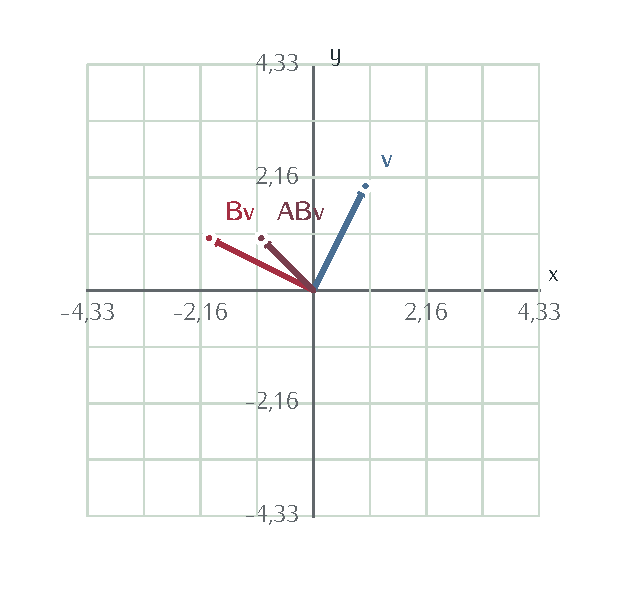
\includegraphics[width=\linewidth,height=94mm,keepaspectratio]{figure/fc706a09269f291fa.pdf}\FigureCaption{2.09 \(\cdot\) esempio 1 \(\cdot\) Ordine \(B\) poi \(A\)}\end{FigureBlock}
\begin{FigureBlock}\centering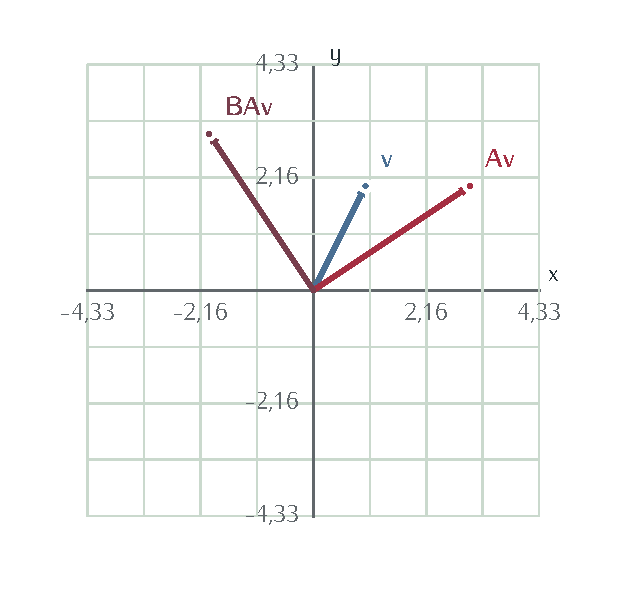
\includegraphics[width=\linewidth,height=94mm,keepaspectratio]{figure/f2664342f4142fb5f.pdf}\FigureCaption{2.09 \(\cdot\) esempio 1 \(\cdot\) Ordine \(A\) poi \(B\)}\end{FigureBlock}

\phantomsection\label{c2-composizione-example-1-step-1}
\BookHeading{01 Leggere le colonne}

\MathBlock{004100652081003D00280031003B0020003000291D40003B0020004100652082003D00280031003B0020003100291D40}{Ae_{1}=(1;\allowbreak \ 0)^{T};\allowbreak \ Ae_{2}=(1;\allowbreak \ 1)^{T}}

Le colonne sono le immagini dei due assi canonici e determinano la trasformazione.\par


\phantomsection\label{c2-composizione-example-1-step-2}
\BookHeading{02 Calcolare Av, componente 1}

\MathBlock{00280031002900B70028003100290020002B002000280031002900B7002800320029003D0033}{(1)\cdot (1)\ +\ (1)\cdot (2)=3}

Ogni riga viene moltiplicata per la colonna delle coordinate di v.\par


\phantomsection\label{c2-composizione-example-1-step-3}
\BookHeading{03 Calcolare Av, componente 2}

\MathBlock{00280030002900B70028003100290020002B002000280031002900B7002800320029003D0032}{(0)\cdot (1)\ +\ (1)\cdot (2)=2}

Ogni riga viene moltiplicata per la colonna delle coordinate di v.\par


\phantomsection\label{c2-composizione-example-1-step-4}
\BookHeading{04 Applicare \(B\) per primo}

\MathBlock{00420076003D002822120032002C00310029003D0028002D0032003B0020003100291D40}{Bv=(- 2{,}1)=(-2;\allowbreak \ 1)^{T}}
\MathBlock{004100420076003D00280031002900B70028002D003200290020002B002000280031002900B7002800310029003B002000280030002900B70028002D003200290020002B002000280031002900B7002800310029003D0028002D0031003B0020003100291D40}{\text{ABv}=(1)\cdot (-2)\ +\ (1)\cdot (1);\allowbreak \ (0)\cdot (-2)\ +\ (1)\cdot (1)=(-1;\allowbreak \ 1)^{T}}

Il vettore ruotato Bv diventa l'ingresso di \(A\).\par


\phantomsection\label{c2-composizione-example-1-step-5}
\BookHeading{05 Applicare \(A\) per primo}

\MathBlock{00410076003D00280033003B0020003200291D40}{Av=(3;\allowbreak \ 2)^{T}}
\MathBlock{004200410076003D00280030002900B70028003300290020002B00200028002D0031002900B7002800320029003B002000280031002900B70028003300290020002B002000280030002900B7002800320029003D0028002D0032003B0020003300291D40}{\text{BAv}=(0)\cdot (3)\ +\ (-1)\cdot (2);\allowbreak \ (1)\cdot (3)\ +\ (0)\cdot (2)=(-2;\allowbreak \ 3)^{T}}

L'immagine Av già calcolata diventa l'ingresso di \(B\).\par


\phantomsection\label{c2-composizione-example-1-step-6}
\BookHeading{06 Confrontare le matrici dei due ordini}

\MathBlock{00410042003D005B005B0031002C0020002D0031005D002C0020005B0031002C00200030005D005D003B002000420041003D005B005B0030002C0020002D0031005D002C0020005B0031002C00200031005D005D}{AB=\begin{pmatrix}1&-1\\1&0\end{pmatrix};\allowbreak \ BA=\begin{pmatrix}0&-1\\1&1\end{pmatrix}}
\MathBlock{00280041004222120042004100290076003D00280031003B0020002D003200291D40}{(AB- BA)v=(1;\allowbreak \ -2)^{T}}

Il prodotto di matrici riassume i due passaggi senza perdere l'ordine.\par


\BookHeading{Interpretazione}

ABv e BAv sono diversi sul medesimo ingresso: il taglio agisce su componenti che la rotazione scambia.\par


\Needspace{.36\textheight}\phantomsection\label{c2-composizione-example-2}
{\sffamily\small\color{Accent} ESEMPIO SVOLTO 2\par}
\BookHeading{Dilatazione uniforme e rotazione commutano}
Dati \(A=\)\(\begin{pmatrix}2&0\\0&2\end{pmatrix}\), \(v=(2\); \(-1)^{T}\). \(B=\)\(\begin{pmatrix}0&- 1\\1&0\end{pmatrix}\) è una rotazione di \(90{}^{\circ} \). Confrontiamo i due ordini sullo stesso ingresso.\par


\BookHeading{Geometria e configurazione dell'esempio}
\begin{FigureBlock}\centering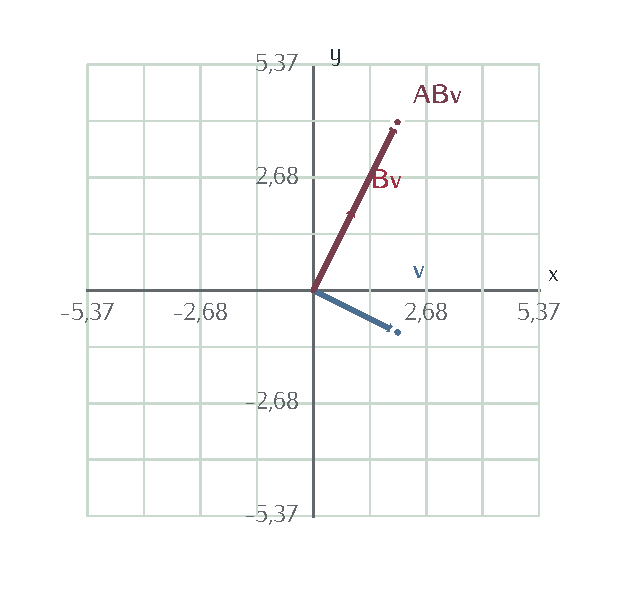
\includegraphics[width=\linewidth,height=94mm,keepaspectratio]{figure/f91d31e07e7443da8.pdf}\FigureCaption{2.09 \(\cdot\) esempio 2 \(\cdot\) Ordine \(B\) poi \(A\)}\end{FigureBlock}
\begin{FigureBlock}\centering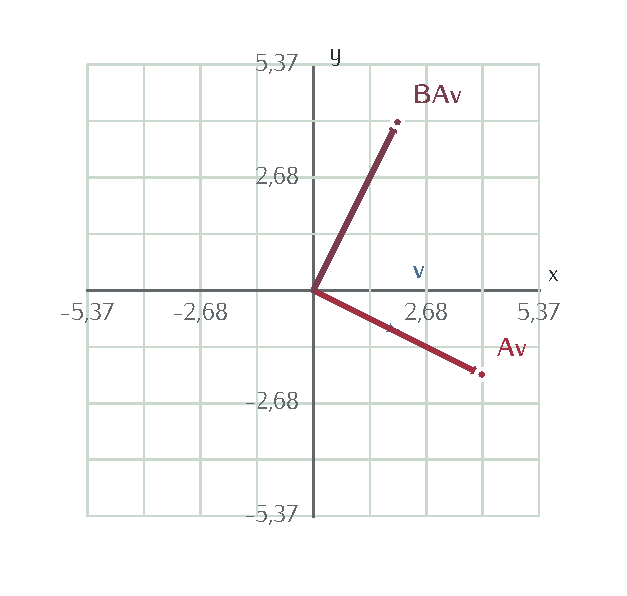
\includegraphics[width=\linewidth,height=94mm,keepaspectratio]{figure/f660b36051c226127.pdf}\FigureCaption{2.09 \(\cdot\) esempio 2 \(\cdot\) Ordine \(A\) poi \(B\)}\end{FigureBlock}

\phantomsection\label{c2-composizione-example-2-step-1}
\BookHeading{01 Leggere le colonne}

\MathBlock{004100652081003D00280032003B0020003000291D40003B0020004100652082003D00280030003B0020003200291D40}{Ae_{1}=(2;\allowbreak \ 0)^{T};\allowbreak \ Ae_{2}=(0;\allowbreak \ 2)^{T}}

Le colonne sono le immagini dei due assi canonici e determinano la trasformazione.\par


\phantomsection\label{c2-composizione-example-2-step-2}
\BookHeading{02 Calcolare Av, componente 1}

\MathBlock{00280032002900B70028003200290020002B002000280030002900B70028002D00310029003D0034}{(2)\cdot (2)\ +\ (0)\cdot (-1)=4}

Ogni riga viene moltiplicata per la colonna delle coordinate di v.\par


\phantomsection\label{c2-composizione-example-2-step-3}
\BookHeading{03 Calcolare Av, componente 2}

\MathBlock{00280030002900B70028003200290020002B002000280032002900B70028002D00310029003D002D0032}{(0)\cdot (2)\ +\ (2)\cdot (-1)=-2}

Ogni riga viene moltiplicata per la colonna delle coordinate di v.\par


\phantomsection\label{c2-composizione-example-2-step-4}
\BookHeading{04 Applicare \(B\) per primo}

\MathBlock{00420076003D00282212002D0031002C00320029003D00280031003B0020003200291D40}{Bv=(- -1{,}2)=(1;\allowbreak \ 2)^{T}}
\MathBlock{004100420076003D00280032002900B70028003100290020002B002000280030002900B7002800320029003B002000280030002900B70028003100290020002B002000280032002900B7002800320029003D00280032003B0020003400291D40}{\text{ABv}=(2)\cdot (1)\ +\ (0)\cdot (2);\allowbreak \ (0)\cdot (1)\ +\ (2)\cdot (2)=(2;\allowbreak \ 4)^{T}}

Il vettore ruotato Bv diventa l'ingresso di \(A\).\par


\phantomsection\label{c2-composizione-example-2-step-5}
\BookHeading{05 Applicare \(A\) per primo}

\MathBlock{00410076003D00280034003B0020002D003200291D40}{Av=(4;\allowbreak \ -2)^{T}}
\MathBlock{004200410076003D00280030002900B70028003400290020002B00200028002D0031002900B70028002D00320029003B002000280031002900B70028003400290020002B002000280030002900B70028002D00320029003D00280032003B0020003400291D40}{\text{BAv}=(0)\cdot (4)\ +\ (-1)\cdot (-2);\allowbreak \ (1)\cdot (4)\ +\ (0)\cdot (-2)=(2;\allowbreak \ 4)^{T}}

L'immagine Av già calcolata diventa l'ingresso di \(B\).\par


\phantomsection\label{c2-composizione-example-2-step-6}
\BookHeading{06 Confrontare le matrici dei due ordini}

\MathBlock{00410042003D005B005B0030002C0020002D0032005D002C0020005B0032002C00200030005D005D003B002000420041003D005B005B0030002C0020002D0032005D002C0020005B0032002C00200030005D005D}{AB=\begin{pmatrix}0&-2\\2&0\end{pmatrix};\allowbreak \ BA=\begin{pmatrix}0&-2\\2&0\end{pmatrix}}
\MathBlock{00280041004222120042004100290076003D00280030003B0020003000291D40}{(AB- BA)v=(0;\allowbreak \ 0)^{T}}

Il prodotto di matrici riassume i due passaggi senza perdere l'ordine.\par


\BookHeading{Interpretazione}

\(AB=BA\) perché una dilatazione uniforme moltiplica entrambe le coordinate dello stesso fattore. La coincidenza è verificata sull'intera matrice.\par


\Needspace{7\baselineskip}
\BookHeading{Il passaggio successivo}
La composizione consente anche di convertire coordinate, applicare un operatore e riconvertire l'uscita. Questa successione costruirà la matrice in una nuova base.\par


% Authoritative exercise source. Preserve all derivations and diagrams.

\ExerciseStart{G2.07}{Confrontare due ordini di composizione}{Consolidamento}

\BookHeading{Problema, dati e obiettivo}

Siano \(A=\begin{pmatrix}0&-1\\1&0\end{pmatrix}\), \(B=\begin{pmatrix}1&1\\0&1\end{pmatrix}\) e \(u=(1,1)^T\). Calcolare AB, BA e le rispettive azioni. A è una rotazione di \(90^\circ\), B uno scorrimento orizzontale.

\ExTheory{\ExRef{c2-composizione}{2.09}}{Nel prodotto AB, B agisce per prima sul vettore. Ogni elemento soddisfa \((AB)_{ij}=\sum_kA_{ik}B_{kj}\). La composizione dipende dall’ordine quando \(AB\ne BA\).}

\ExPrediction{Lo scorrimento modifica la coordinata orizzontale usando quella verticale. La rotazione scambia il ruolo geometrico delle due coordinate: prevedere due percorsi differenti.}

\ExFigure{\begin{tikzpicture}[>=Stealth,exlabel]
\node[exbox] (n0) at (0.0,0.0) {$u=(1,1)$};\node[exbox] (n1) at (3.6,0.0) {$Bu=(2,1)$};\draw[exother] (n0)--(n1);\node[exbox] (n2) at (7.2,0.0) {$ABu=(-1,2)$};\draw[exother] (n1)--(n2);
\end{tikzpicture}}{Primo percorso: scorrimento seguito da rotazione.}


\begin{ExTasks}

\item Calcolare Bu e poi A(Bu).

\item Calcolare Au e poi B(Au).

\item Svolgere i quattro elementi di AB.

\item Svolgere i quattro elementi di BA.

\item Confrontare risultati, norme e commutatore applicato a u.

\end{ExTasks}

\ExSolution

\ExStep{Eseguire prima lo scorrimento}

\ExEq{Bu&=\colv{1+1\\1}=\colv{2\\1},\\A(Bu)&=\colv{0\cdot2-1\cdot1\\1\cdot2+0\cdot1}=\colv{-1\\2}.}

\ExStep{Eseguire prima la rotazione}

\ExEq{Au&=\colv{-1\\1},\\B(Au)&=\colv{-1+1\\1}=\colv{0\\1}.}

\ExStep{Costruire AB}

\ExEq{AB&=\begin{pmatrix}0\cdot1+(-1)0&0\cdot1+(-1)1\\1\cdot1+0\cdot0&1\cdot1+0\cdot1\end{pmatrix}
=\begin{pmatrix}0&-1\\1&1\end{pmatrix}.}
Il prodotto con u dà \((0-1,1+1)^T=(-1,2)^T\).

\ExStep{Costruire BA}

\ExEq{BA&=\begin{pmatrix}1\cdot0+1\cdot1&1(-1)+1\cdot0\\0\cdot0+1\cdot1&0(-1)+1\cdot0\end{pmatrix}
=\begin{pmatrix}1&-1\\1&0\end{pmatrix}.}
Il prodotto con u dà \((1-1,1+0)^T=(0,1)^T\).

\ExStep{Quantificare la differenza}

\ExEq{AB-BA&=\begin{pmatrix}-1&0\\0&1\end{pmatrix},\\(AB-BA)u&=\colv{-1\\1}.}
Le norme finali sono \(\sqrt5\) e 1. A conserva le lunghezze; B può cambiarle, perché è uno scorrimento e non una matrice ortogonale.

\par\noindent\begin{minipage}{\linewidth}
\ExFigure{\begin{tikzpicture}[>=Stealth,exlabel]
\draw[exaxis] (-1.35,0)--(1.55,0) node[right] {$x_1$};\draw[exaxis] (0,-0.35)--(0,2.55) node[above] {$x_2$};\draw[->,Ink,line width=1.1pt] (0,0)--(1,1) node[anchor=south west] {$ u $};\draw[->,Accent,line width=1.1pt] (0,0)--(-1,2) node[anchor=south west] {$ ABu $};\draw[->,Secondary,line width=1.1pt] (0,0)--(0,1) node[anchor=south west] {$ BAu $};
\end{tikzpicture}}{I risultati dei due percorsi appartengono a direzioni e hanno lunghezze differenti.}


\ExInterpret{L’ordine degli operatori ha un significato geometrico verificabile. La stessa regola di lettura dei prodotti verrà usata per le porte quantistiche, che soddisfano inoltre l’unitarietà.}

\ExLab{Nella sezione 2.09 confrontare i due ordini nel diagramma di composizione. Se si usano le matrici dell’esercizio nello strumento delle matrici, conservare lo stesso ingresso u per entrambi i percorsi.}


\end{minipage}

\Needspace{.43\textheight}
\section{Descrivere una trasformazione in un'altra base}
\phantomsection\label{c2-cambio-base}

{\sffamily\small\color{Ink!70} Riferimento alle slide: p. 138.\par}

{\sffamily\small\color{Ink!70} Laboratorio locale: \nolinkurl{index.html#capitolo-2/cambio-base}\par}

\BookHeading{Definizioni e costruzione}
Il vettore fisso può avere coordinate differenti. Una matrice descritta nella nuova base deve convertire le coordinate all'ingresso e all'uscita.\par

La matrice \(B\) converte coordinate nella nuova base in coordinate canoniche. La sua inversa \(B^{-1}\) soddisfa \(B^{-1}B=BB^{-1}=I\), dove I conserva ogni vettore. Per \(B=\)\(\begin{pmatrix}a&b\\c&d\end{pmatrix}\) con \(ad- bc\ne 0\), \(B^{-1}=(1/(ad- bc))\)\(\begin{pmatrix}d&- b\\- c&a\end{pmatrix}\). Una base dipendente non possiede questa conversione inversa.\par

Per descrivere \(A\) nella nuova base si converte l'ingresso con \(B\), si applica \(A\) e si riporta l'uscita nella nuova base mediante \(B^{-1}\). Il prodotto \([A]B=B^{-1}AB\) conserva l'azione geometrica di \(A\) e cambia i numeri che la descrivono. Per leggere la lunghezza in una base obliqua si può sempre ricostruire Bc e calcolarne la norma canonica; la norma delle sole coordinate c non coincide generalmente con quella di Bc.\par


\MathBlock{005B0041005D0042003D0042207B00B900410042002E}{[A]B=B^{-1}AB.}

\BookHeading{Come leggere le figure}
Piano reale; il cambio di coordinate conserva il vettore geometrico.\par


\Needspace{.36\textheight}\phantomsection\label{c2-cambio-base-example-1}
{\sffamily\small\color{Accent} ESEMPIO SVOLTO 1\par}
\BookHeading{Conversione prima e dopo \(A\)}
Dati \(b_{1}=(1{,}0)\), \(b_{2}=(1{,}1)\), \(B=\)\(\begin{pmatrix}1&1\\0&1\end{pmatrix}\), \(v=(3\); \(2)^{T}\). L'operatore in coordinate canoniche è \(A=\)\(\begin{pmatrix}2&0\\0&1\end{pmatrix}\). Riprendiamo la base obliqua per descriverne l'azione.\par


\BookHeading{Geometria e configurazione dell'esempio}
\begin{FigureBlock}\centering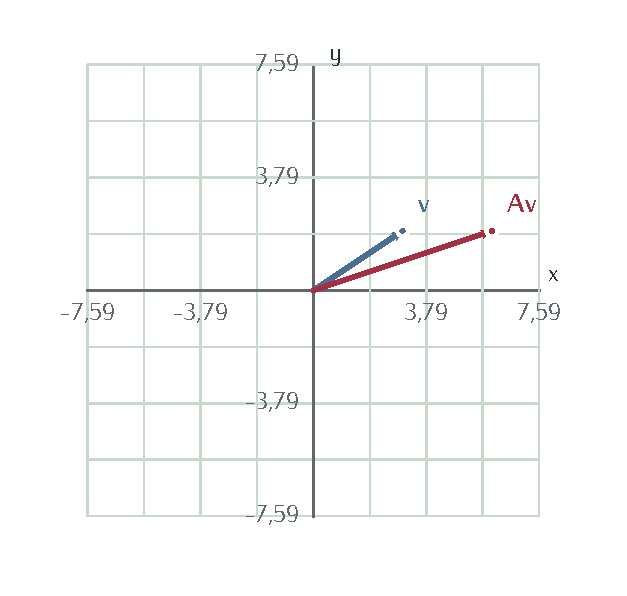
\includegraphics[width=\linewidth,height=94mm,keepaspectratio]{figure/f7caf7cd56947fa3b.pdf}\FigureCaption{2.10 \(\cdot\) esempio 1 \(\cdot\) Vettore e trasformazione nel piano canonico}\end{FigureBlock}
\begin{FigureBlock}\centering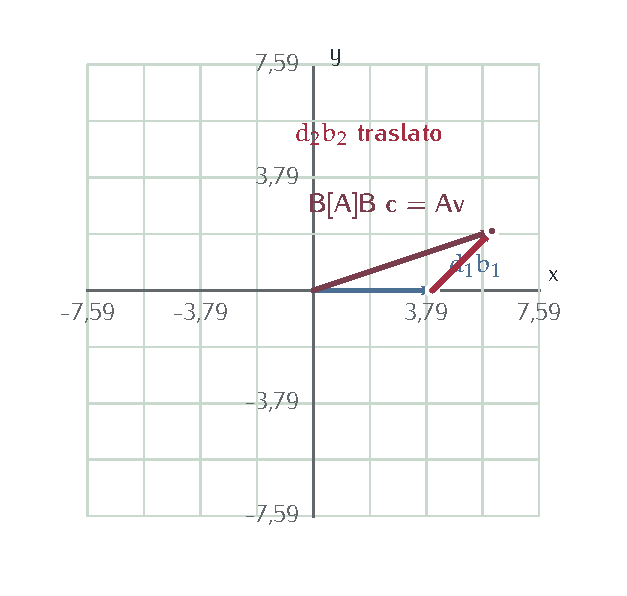
\includegraphics[width=\linewidth,height=94mm,keepaspectratio]{figure/f5e628e1d43358214.pdf}\FigureCaption{2.10 \(\cdot\) esempio 1 \(\cdot\) Ricomposizione dell'uscita in coordinate canoniche}\end{FigureBlock}

\phantomsection\label{c2-cambio-base-example-1-step-1}
\BookHeading{01 Ricostruire il vettore}

\MathBlock{00420063003D0063208100280031002C00300029002B0063208200280031002C00310029003D002800632081002B003100632082002C006320820029003D00280033003B0020003200291D40}{Bc=c_{1}(1{,}0)+c_{2}(1{,}1)=(c_{1}+1c_{2},\allowbreak c_{2})=(3;\allowbreak \ 2)^{T}}

Le coordinate cercate sono i coefficienti \(c_{1},\allowbreak c_{2}\).\par


\phantomsection\label{c2-cambio-base-example-1-step-2}
\BookHeading{02 Risolvere il sistema}

\MathBlock{00632082003D0032003B002000632081003D00332212003100B70032003D0031003B0020005B0076005D0042003D00280031003B0020003200291D40}{c_{2}=2;\allowbreak \ c_{1}=3- 1\cdot 2=1;\allowbreak \ [v]B=(1;\allowbreak \ 2)^{T}}

La seconda equazione determina \(c_{2}\); la prima determina poi \(c_{1}\) in modo unico.\par


\phantomsection\label{c2-cambio-base-example-1-step-3}
\BookHeading{03 Verificare la somma}

\MathBlock{0063208100622081003D00280031003B0020003000291D40003B00200063208200622082003D00280032003B0020003200291D40}{c_{1}b_{1}=(1;\allowbreak \ 0)^{T};\allowbreak \ c_{2}b_{2}=(2;\allowbreak \ 2)^{T}}
\MathBlock{0063208100622081002B0063208200622082003D00280033003B0020003200291D40}{c_{1}b_{1}+c_{2}b_{2}=(3;\allowbreak \ 2)^{T}}

I contributi hanno le direzioni della base, mentre la loro somma coincide con v.\par


\phantomsection\label{c2-cambio-base-example-1-step-4}
\BookHeading{04 Applicare \(A\) in coordinate canoniche}

\MathBlock{00410076003D0028003200B70033002C00320029003D00280036003B0020003200291D40}{Av=(2\cdot 3{,}2)=(6;\allowbreak \ 2)^{T}}
\MathBlock{00410042003D005B005B0032002C0032005D002C005B0030002C0031005D005D}{AB=\begin{pmatrix}2&2\\0&1\end{pmatrix}}

\(A\) raddoppia la componente orizzontale di ciascun vettore della base.\par


\phantomsection\label{c2-cambio-base-example-1-step-5}
\BookHeading{05 Convertire le immagini nella base \(B\)}

\MathBlock{0042207B00B9003D005B005B0031002C002D0031005D002C005B0030002C0031005D005D}{B^{-1}=\begin{pmatrix}1&-1\\0&1\end{pmatrix}}
\MathBlock{005B0041005D0042003D0042207B00B900410042003D005B005B0032002C0031005D002C005B0030002C0031005D005D}{[A]B=B^{-1}AB=\begin{pmatrix}2&1\\0&1\end{pmatrix}}
\MathBlock{005B00410076005D0042003D005B0041005D004200200063003D0028003200B70031002B003100B70032002C00320029003D00280034003B0020003200291D40}{[Av]B=[A]B\ c=(2\cdot 1+1\cdot 2{,}2)=(4;\allowbreak \ 2)^{T}}

Il fattore \(B\) converte l'ingresso, \(A\) trasforma il vettore, \(B^{-1}\) restituisce le coordinate di uscita.\par


\phantomsection\label{c2-cambio-base-example-1-step-6}
\BookHeading{06 Ricomporre la stessa uscita}

\MathBlock{0042005B00410076005D0042003D00280034002B003100B70032002C00320029003D00280036003B0020003200291D40003D00410076}{B[Av]B=(4+1\cdot 2{,}2)=(6;\allowbreak \ 2)^{T}=Av}

Le due strade producono lo stesso punto nel piano canonico.\par


\BookHeading{Interpretazione}

\(A\) porta v in (6; \(2)^{T}\); [A]B porta le coordinate c in (4; \(2)^{T}\). La ricostruzione con \(B\) verifica che l'azione geometrica coincide.\par


\Needspace{.36\textheight}\phantomsection\label{c2-cambio-base-example-2}
{\sffamily\small\color{Accent} ESEMPIO SVOLTO 2\par}
\BookHeading{Stessa dilatazione, base più obliqua}
Dati \(b_{1}=(1{,}0)\), \(b_{2}=(2{,}1)\), \(B=\)\(\begin{pmatrix}1&2\\0&1\end{pmatrix}\), \(v=(5\); \(2)^{T}\). L'operatore in coordinate canoniche è \(A=\)\(\begin{pmatrix}2&0\\0&1\end{pmatrix}\). Riprendiamo la base obliqua per descriverne l'azione.\par


\BookHeading{Geometria e configurazione dell'esempio}
\begin{FigureBlock}\centering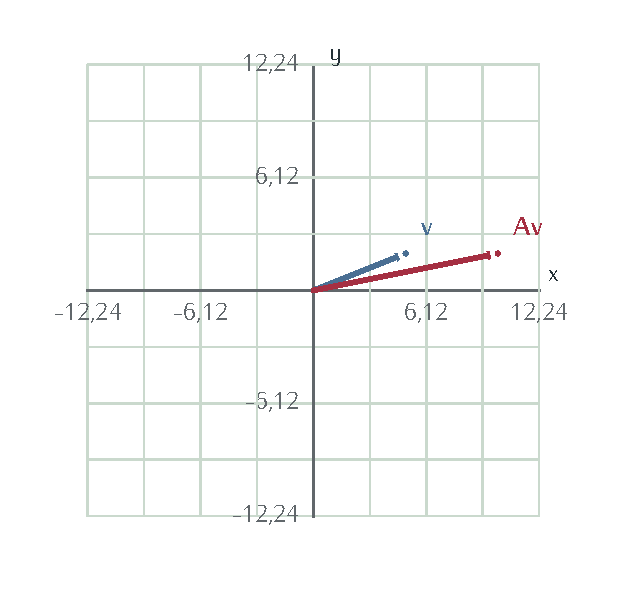
\includegraphics[width=\linewidth,height=94mm,keepaspectratio]{figure/f909200864f7593fb.pdf}\FigureCaption{2.10 \(\cdot\) esempio 2 \(\cdot\) Vettore e trasformazione nel piano canonico}\end{FigureBlock}
\begin{FigureBlock}\centering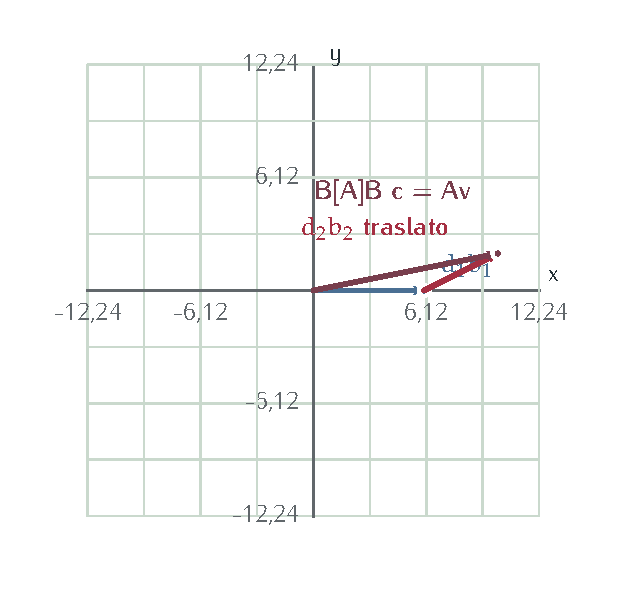
\includegraphics[width=\linewidth,height=94mm,keepaspectratio]{figure/f11415a1b323f455c.pdf}\FigureCaption{2.10 \(\cdot\) esempio 2 \(\cdot\) Ricomposizione dell'uscita in coordinate canoniche}\end{FigureBlock}

\phantomsection\label{c2-cambio-base-example-2-step-1}
\BookHeading{01 Ricostruire il vettore}

\MathBlock{00420063003D0063208100280031002C00300029002B0063208200280032002C00310029003D002800632081002B003200632082002C006320820029003D00280035003B0020003200291D40}{Bc=c_{1}(1{,}0)+c_{2}(2{,}1)=(c_{1}+2c_{2},\allowbreak c_{2})=(5;\allowbreak \ 2)^{T}}

Le coordinate cercate sono i coefficienti \(c_{1},\allowbreak c_{2}\).\par


\phantomsection\label{c2-cambio-base-example-2-step-2}
\BookHeading{02 Risolvere il sistema}

\MathBlock{00632082003D0032003B002000632081003D00352212003200B70032003D0031003B0020005B0076005D0042003D00280031003B0020003200291D40}{c_{2}=2;\allowbreak \ c_{1}=5- 2\cdot 2=1;\allowbreak \ [v]B=(1;\allowbreak \ 2)^{T}}

La seconda equazione determina \(c_{2}\); la prima determina poi \(c_{1}\) in modo unico.\par


\phantomsection\label{c2-cambio-base-example-2-step-3}
\BookHeading{03 Verificare la somma}

\MathBlock{0063208100622081003D00280031003B0020003000291D40003B00200063208200622082003D00280034003B0020003200291D40}{c_{1}b_{1}=(1;\allowbreak \ 0)^{T};\allowbreak \ c_{2}b_{2}=(4;\allowbreak \ 2)^{T}}
\MathBlock{0063208100622081002B0063208200622082003D00280035003B0020003200291D40}{c_{1}b_{1}+c_{2}b_{2}=(5;\allowbreak \ 2)^{T}}

I contributi hanno le direzioni della base, mentre la loro somma coincide con v.\par


\phantomsection\label{c2-cambio-base-example-2-step-4}
\BookHeading{04 Applicare \(A\) in coordinate canoniche}

\MathBlock{00410076003D0028003200B70035002C00320029003D002800310030003B0020003200291D40}{Av=(2\cdot 5{,}2)=(10;\allowbreak \ 2)^{T}}
\MathBlock{00410042003D005B005B0032002C0034005D002C005B0030002C0031005D005D}{AB=\begin{pmatrix}2&4\\0&1\end{pmatrix}}

\(A\) raddoppia la componente orizzontale di ciascun vettore della base.\par


\phantomsection\label{c2-cambio-base-example-2-step-5}
\BookHeading{05 Convertire le immagini nella base \(B\)}

\MathBlock{0042207B00B9003D005B005B0031002C002D0032005D002C005B0030002C0031005D005D}{B^{-1}=\begin{pmatrix}1&-2\\0&1\end{pmatrix}}
\MathBlock{005B0041005D0042003D0042207B00B900410042003D005B005B0032002C0032005D002C005B0030002C0031005D005D}{[A]B=B^{-1}AB=\begin{pmatrix}2&2\\0&1\end{pmatrix}}
\MathBlock{005B00410076005D0042003D005B0041005D004200200063003D0028003200B70031002B003200B70032002C00320029003D00280036003B0020003200291D40}{[Av]B=[A]B\ c=(2\cdot 1+2\cdot 2{,}2)=(6;\allowbreak \ 2)^{T}}

Il fattore \(B\) converte l'ingresso, \(A\) trasforma il vettore, \(B^{-1}\) restituisce le coordinate di uscita.\par


\phantomsection\label{c2-cambio-base-example-2-step-6}
\BookHeading{06 Ricomporre la stessa uscita}

\MathBlock{0042005B00410076005D0042003D00280036002B003200B70032002C00320029003D002800310030003B0020003200291D40003D00410076}{B[Av]B=(6+2\cdot 2{,}2)=(10;\allowbreak \ 2)^{T}=Av}

Le due strade producono lo stesso punto nel piano canonico.\par


\BookHeading{Interpretazione}

\(A\) porta v in (10; \(2)^{T}\); [A]B porta le coordinate c in (6; \(2)^{T}\). La ricostruzione con \(B\) verifica che l'azione geometrica coincide.\par


\Needspace{7\baselineskip}
\BookHeading{Il passaggio successivo}
Il cambio di base ha richiesto l'inversa. L'aggiunto è un'operazione differente, costruita per trasferire una matrice fra i due argomenti del prodotto interno.\par


% Authoritative exercise source. Preserve all derivations and diagrams.

\ExerciseStart{G2.08}{Cambiare coordinate mantenendo lo stesso oggetto}{Consolidamento}

\BookHeading{Problema, dati e obiettivo}

La nuova base è \(f_1=(1,1)^T\), \(f_2=(1,-1)^T\). Per \(u=(3,1)^T\) e \(A=\operatorname{diag}(2,1)\), calcolare coordinate nella nuova base, matrice trasformata e risultato dell’operazione nei due sistemi di coordinate.

\ExTheory{\ExRef{c2-cambio-base}{2.10}}{La matrice \(S=(f_1\ f_2)\) porta le coordinate nuove in quelle canoniche: \(u=S[u]_f\). Pertanto \([u]_f=S^{-1}u\) e \([A]_f=S^{-1}AS\). La base scelta è ortogonale ma i suoi vettori hanno norma \(\sqrt2\).}

\ExPrediction{Il punto u resta lo stesso quando se ne cambiano le coordinate. Il rettangolo di dilatazione descritto da A appare con termini fuori diagonale nella base inclinata.}

\ExFigure{\begin{tikzpicture}[>=Stealth,exlabel]
\draw[exaxis] (-0.35,0)--(3.55,0) node[right] {$x_1$};\draw[exaxis] (0,-1.35)--(0,1.55) node[above] {$x_2$};\draw[->,Accent,line width=1.1pt] (0,0)--(1,1) node[anchor=south west] {$ f_1 $};\draw[->,Secondary,line width=1.1pt] (0,0)--(1,-1) node[anchor=north west] {$ f_2 $};\draw[->,Ink,line width=1.1pt] (0,0)--(3,1) node[anchor=south west] {$ u $};
\end{tikzpicture}}{Base inclinata e punto u nello stesso piano geometrico.}


\begin{ExTasks}

\item Costruire S e verificarne l’inversa.

\item Calcolare le nuove coordinate di u e ricostruirlo.

\item Calcolare AS e poi \(S^{-1}AS\).

\item Applicare la matrice trasformata.

\item Riportare il risultato nella base canonica e controllare la norma usando la metrica corretta.

\end{ExTasks}

\ExSolution

\ExStep{Verificare l’inversa}

\ExEq{S&=\begin{pmatrix}1&1\\1&-1\end{pmatrix},\\S^2&=\begin{pmatrix}1+1&1-1\\1-1&1+1\end{pmatrix}=2I,\qquad S^{-1}=S/2.}

\ExStep{Cambiare le coordinate}

\ExEq{[u]_f&=\tfrac12\colv{3+1\\3-1}=\colv{2\\1},\\S[u]_f&=\colv{2+1\\2-1}=\colv{3\\1}.}

\ExStep{Trasformare l’operatore}

\ExEq{AS&=\begin{pmatrix}2&2\\1&-1\end{pmatrix},\\S^{-1}AS&=\tfrac12\begin{pmatrix}2+1&2-1\\2-1&2+1\end{pmatrix}
=\tfrac12\begin{pmatrix}3&1\\1&3\end{pmatrix}.}

\ExStep{Agire nelle nuove coordinate}

\ExEq{[Au]_f&=\tfrac12\colv{3\cdot2+1\cdot1\\1\cdot2+3\cdot1}
=\colv{7/2\\5/2},\\S[Au]_f&=\colv{7/2+5/2\\7/2-5/2}=\colv{6\\1}.}

\ExStep{Confrontare la via diretta e la metrica}

Il calcolo canonico dà \(Au=(2\cdot3,1\cdot1)^T=(6,1)^T\). Per le coordinate della base f, \(S^TS=2I\): quindi \(\|u\|^2=2(2^2+1^2)=10=3^2+1^2\). Analogamente \(2[(7/2)^2+(5/2)^2]=37=6^2+1^2\).

\par\noindent\begin{minipage}{\linewidth}
\ExFigure{\begin{tikzpicture}[>=Stealth,exlabel]
\node[exbox] (n0) at (0.0,0.0) {$[u]_f=(2,1)$};\node[exbox] (n1) at (3.6,0.0) {$[Au]_f=(7/2,5/2)$};\draw[exother] (n0)--(n1);\node[exbox] (n2) at (7.2,0.0) {$Au=(6,1)$};\draw[exother] (n1)--(n2);
\end{tikzpicture}}{Il cambio di coordinate e l’azione dell’operatore sono passaggi distinti.}


\ExInterpret{Le coordinate dipendono dalla base; il vettore geometrico e l’azione di A restano definiti indipendentemente da essa. La metrica \(S^TS\) mantiene corretta la lettura delle lunghezze in una base non normalizzata.}

\ExLab{Nella sezione 2.10 seguire i due percorsi del cambio di base. Confrontare il punto ottenuto applicando prima A con quello ricostruito dopo \(S^{-1}AS\), usando sempre le stesse colonne di S.}


\end{minipage}

\Needspace{.43\textheight}
\section{Aggiunto e conservazione della norma}
\phantomsection\label{c2-aggiunto}

{\sffamily\small\color{Ink!70} Riferimento alle slide: p. 89.\par}

{\sffamily\small\color{Ink!70} Laboratorio locale: \nolinkurl{index.html#capitolo-2/aggiunto}\par}

\BookHeading{Definizioni e costruzione}
Trasporre e coniugare permette di trasferire una matrice nel prodotto interno. La condizione \(U{}^{\dagger} U=I\) esprime la conservazione di tutti i prodotti interni.\par

L'aggiunto \(A{}^{\dagger} \) si ottiene trasponendo \(A\), cioè scambiandone righe e colonne, e coniugando ogni elemento: \((A{}^{\dagger} )_{ij}=(A_{ji}){}^{*}\). Questa costruzione soddisfa \(\langle u,\allowbreak Av\rangle =\langle A{}^{\dagger} u,\allowbreak v\rangle \). Infatti \(\langle u,\allowbreak Av\rangle =\sum _{ij}\) \(u_{i}{}^{*}\) Aij \(v_{j}\), mentre la componente j di \(A{}^{\dagger} u\) è \(\sum i\) \(A_{ij}{}^{*}\) \(u_{i}\); coniugandola nel prodotto interno si recupera la stessa somma.\par

Una matrice hermitiana soddisfa \(A{}^{\dagger} =A\); una matrice unitaria soddisfa \(U{}^{\dagger} U=I\). Nel secondo caso \(\langle Uu,\allowbreak Uv\rangle =u{}^{\dagger} U{}^{\dagger} Uv=u{}^{\dagger} v=\langle u,\allowbreak v\rangle \), perciò norme e ortogonalità sono conservate. Le condizioni sono diverse: diag(2,1) è hermitiana e cambia alcune norme; diag(1,i) è unitaria e differisce dal proprio aggiunto. Gli esempi mostrano separatamente la necessità della trasposizione, del coniugio e del controllo \(U{}^{\dagger} U\).\par


\MathBlock{00412020003D00280041002A00291D40003B0020005500200075006E00690074006100720069006F002021D40020005520200055003D0049002E}{A{}^{\dagger} =(A{}^{*})^{T};\allowbreak \ U\ \text{unitario}\ \Leftrightarrow \ U{}^{\dagger} U=I.}

\BookHeading{Come leggere le figure}
Componenti complesse e norme; una matrice hermitiana può anche essere unitaria.\par


\Needspace{.36\textheight}\phantomsection\label{c2-aggiunto-example-1}
{\sffamily\small\color{Accent} ESEMPIO SVOLTO 1\par}
\BookHeading{Trasposizione e coniugio entrambi necessari}
Dati \(A=\)\(\begin{pmatrix}1&i\\0&1\end{pmatrix}\), \(u=(1,\allowbreak i)^{T}\), \(v=(1{,}1)^{T}\).\par


\BookHeading{Geometria e configurazione dell'esempio}
\begin{FigureBlock}\begin{minipage}[t]{.485\linewidth}\centering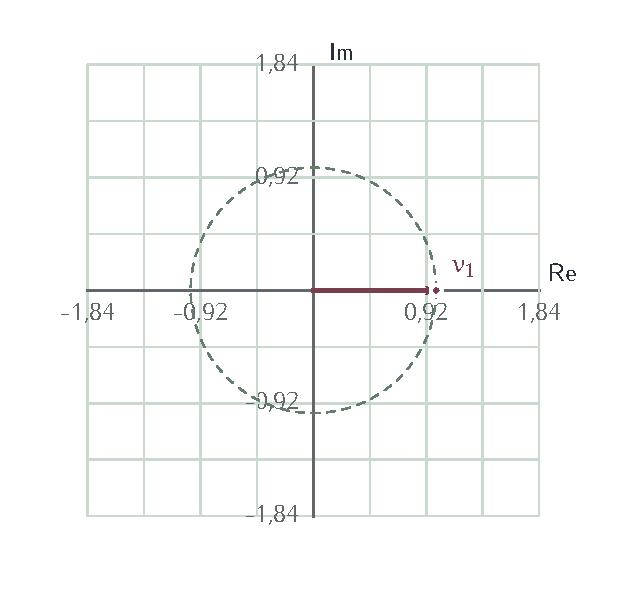
\includegraphics[width=\linewidth,height=63mm,keepaspectratio]{figure/fb10017771667f6a8.pdf}\par{\sffamily\footnotesize \(v_{1}\)\par}\end{minipage}\hfill\begin{minipage}[t]{.485\linewidth}\centering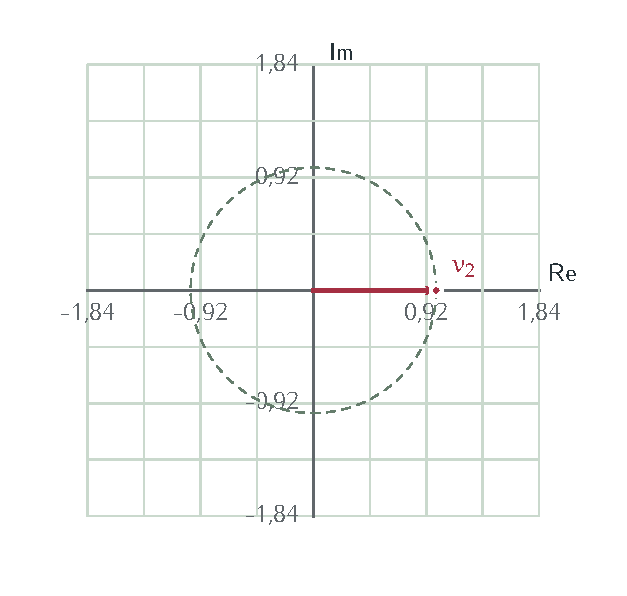
\includegraphics[width=\linewidth,height=63mm,keepaspectratio]{figure/f593923f3bcd9e3c8.pdf}\par{\sffamily\footnotesize \(v_{2}\)\par}\end{minipage}\FigureCaption{2.11 \(\cdot\) esempio 1 \(\cdot\) Componenti prima e dopo \(A\)}\end{FigureBlock}
\begin{FigureBlock}\begin{minipage}[t]{.485\linewidth}\centering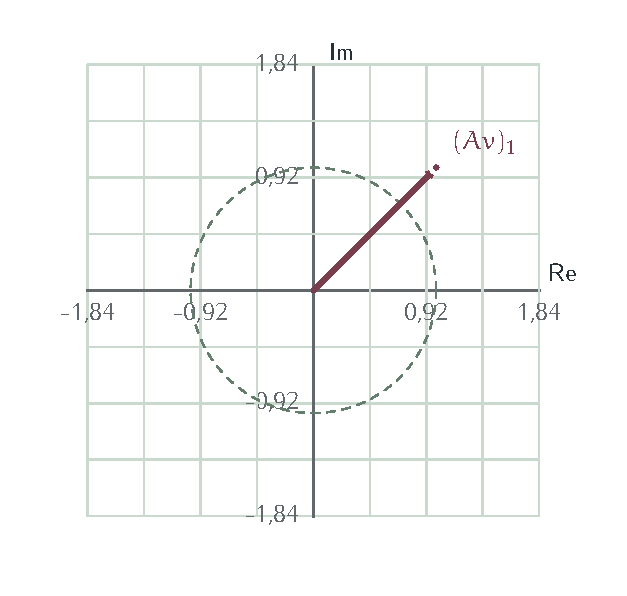
\includegraphics[width=\linewidth,height=63mm,keepaspectratio]{figure/ff8ba0dd06bd82e76.pdf}\par{\sffamily\footnotesize \((Av)_{1}\)\par}\end{minipage}\hfill\begin{minipage}[t]{.485\linewidth}\centering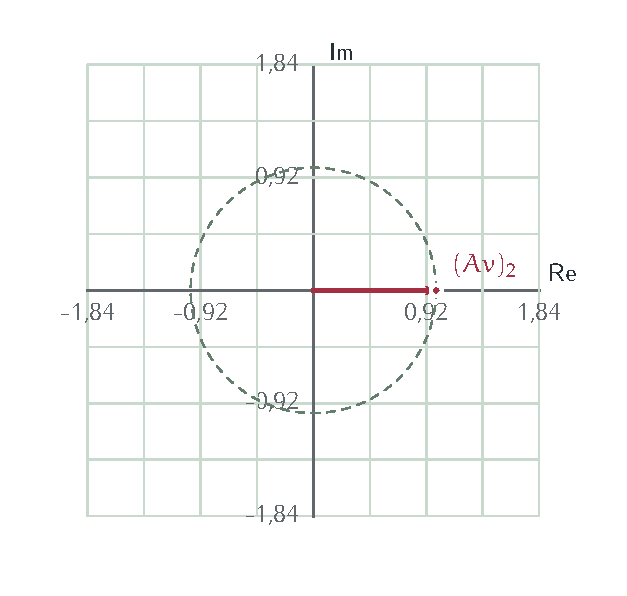
\includegraphics[width=\linewidth,height=63mm,keepaspectratio]{figure/f238c523f6cd8ca9e.pdf}\par{\sffamily\footnotesize \((Av)_{2}\)\par}\end{minipage}\FigureCaption{2.11 \(\cdot\) esempio 1 \(\cdot\) Componenti prima e dopo \(A\)}\end{FigureBlock}

\phantomsection\label{c2-aggiunto-example-1-step-1}
\BookHeading{01 Trasporre e poi coniugare}

\MathBlock{00411D40003D005B005B0031002C00200030005D002C0020005B0069002C00200031005D005D}{A^{T}=\begin{pmatrix}1&0\\i&1\end{pmatrix}}
\MathBlock{00412020003D005B005B0031002C00200030005D002C0020005B22120069002C00200031005D005D}{A{}^{\dagger} =\begin{pmatrix}1&0\\- i&1\end{pmatrix}}

Trasporre sposta l'elemento (r,c) in (c,r); coniugare cambia il segno di ogni parte immaginaria.\par


\phantomsection\label{c2-aggiunto-example-1-step-2}
\BookHeading{02 Verificare la definizione}

\MathBlock{00410076003D002800310020002B00200069003B0020003100291D40003B0020004120200075003D00280031003B0020003000291D40}{Av=(1\ +\ i;\allowbreak \ 1)^{T};\allowbreak \ A{}^{\dagger} u=(1;\allowbreak \ 0)^{T}}
\MathBlock{27E80075002C0041007627E9003D00280031002900B7002800310020002B0020006900290020002B0020002822120069002900B7002800310029003D0031}{\langle u,\allowbreak Av\rangle =(1)\cdot (1\ +\ i)\ +\ (- i)\cdot (1)=1}
\MathBlock{27E8004120200075002C007627E9003D00280031002900B70028003100290020002B002000280030002900B7002800310029003D0031}{\langle A{}^{\dagger} u,\allowbreak v\rangle =(1)\cdot (1)\ +\ (0)\cdot (1)=1}

I due prodotti interni coincidono: l'aggiunto trasferisce \(A\) dal secondo al primo argomento.\par


\phantomsection\label{c2-aggiunto-example-1-step-3}
\BookHeading{03 Distinguere le due proprietà}

\MathBlock{004120200020226000200041}{A{}^{\dagger} \ \ne \ A}
\MathBlock{004120200041003D005B005B0031002C00200069005D002C0020005B22120069002C00200032005D005D22600049}{A{}^{\dagger} A=\begin{pmatrix}1&i\\- i&2\end{pmatrix}\ne I}
\MathBlock{20160076201600B2003D0032003B0020201600410076201600B2003D0033}{\Vert v\Vert ^{2}=2;\allowbreak \ \Vert Av\Vert ^{2}=3}

Hermitianità confronta \(A\) con il suo aggiunto; unitarietà confronta \(A{}^{\dagger} A\) con I. Sono condizioni differenti.\par


\phantomsection\label{c2-aggiunto-example-1-step-4}
\BookHeading{04 Confrontare con una matrice unitaria}

\MathBlock{0055003D005B005B0031002C0030005D002C005B0030002C0069005D005D003B002000552020003D005B005B0031002C0030005D002C005B0030002C22120069005D005D}{U=\begin{pmatrix}1&0\\0&i\end{pmatrix};\allowbreak \ U{}^{\dagger} =\begin{pmatrix}1&0\\0&- i\end{pmatrix}}
\MathBlock{005520200055003D005B005B0031002C0030005D002C005B0030002C00282212006900290069005D005D003D0049003B00200055202022600055}{U{}^{\dagger} U=\begin{pmatrix}1&0\\0&(- i)i\end{pmatrix}=I;\allowbreak \ U{}^{\dagger} \ne U}

Una fase su una coordinata fornisce anche un esempio unitario che non è hermitiano.\par


\BookHeading{Interpretazione}

L'elemento i si sposta sotto la diagonale e diventa \(- i\) nell'aggiunto. \(A\) non è hermitiana né unitaria; \(U\) mostra che l'unitarietà può sussistere senza hermitianità.\par


\Needspace{.36\textheight}\phantomsection\label{c2-aggiunto-example-2}
{\sffamily\small\color{Accent} ESEMPIO SVOLTO 2\par}
\BookHeading{Hermitiana con norma variabile}
Dati \(A=\)\(\begin{pmatrix}2&0\\0&1\end{pmatrix}\), \(u=(1,\allowbreak i)^{T}\), \(v=(1{,}1)^{T}\).\par


\BookHeading{Geometria e configurazione dell'esempio}
\begin{FigureBlock}\begin{minipage}[t]{.485\linewidth}\centering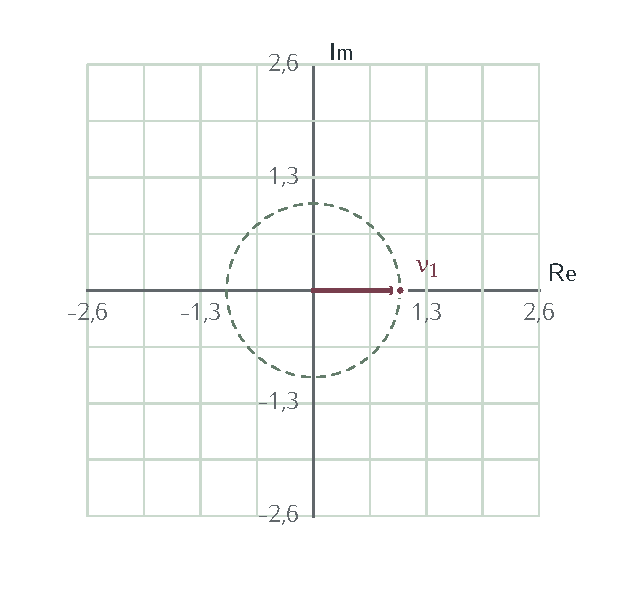
\includegraphics[width=\linewidth,height=63mm,keepaspectratio]{figure/f4258653bf3cd96c2.pdf}\par{\sffamily\footnotesize \(v_{1}\)\par}\end{minipage}\hfill\begin{minipage}[t]{.485\linewidth}\centering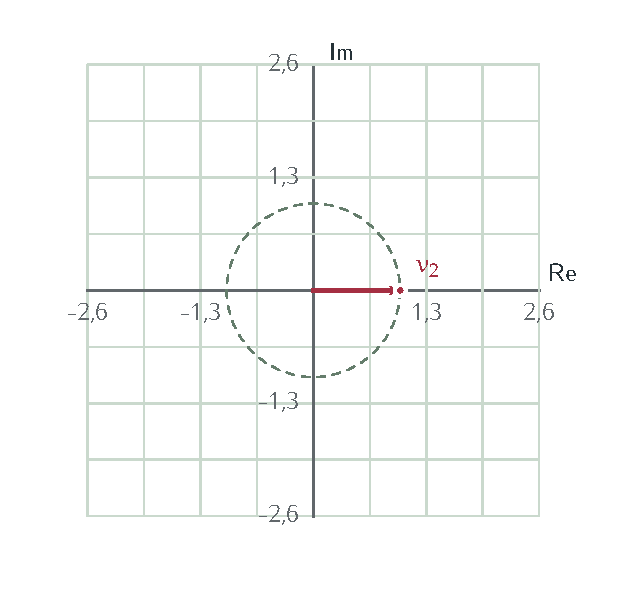
\includegraphics[width=\linewidth,height=63mm,keepaspectratio]{figure/f9ccff265e5c015a1.pdf}\par{\sffamily\footnotesize \(v_{2}\)\par}\end{minipage}\FigureCaption{2.11 \(\cdot\) esempio 2 \(\cdot\) Componenti prima e dopo \(A\)}\end{FigureBlock}
\begin{FigureBlock}\begin{minipage}[t]{.485\linewidth}\centering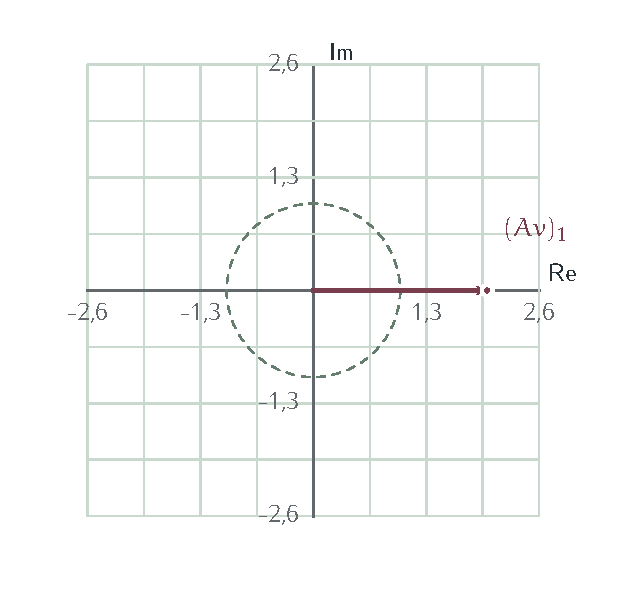
\includegraphics[width=\linewidth,height=63mm,keepaspectratio]{figure/f3c65b92f8638ad0a.pdf}\par{\sffamily\footnotesize \((Av)_{1}\)\par}\end{minipage}\hfill\begin{minipage}[t]{.485\linewidth}\centering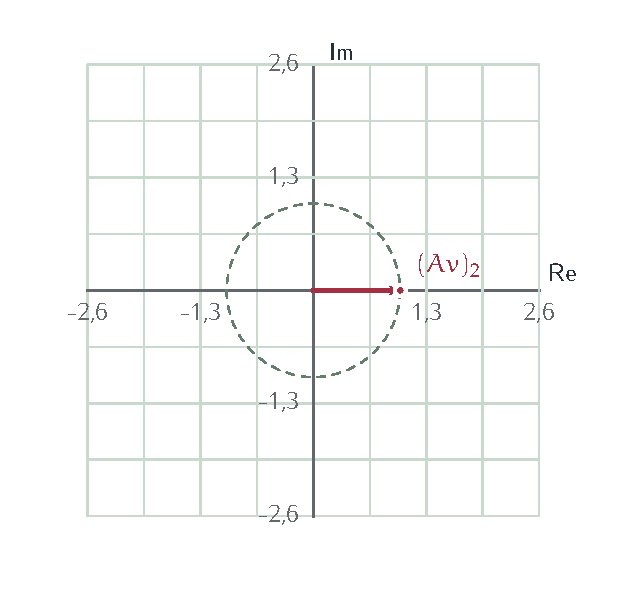
\includegraphics[width=\linewidth,height=63mm,keepaspectratio]{figure/f9879f8a19f7287eb.pdf}\par{\sffamily\footnotesize \((Av)_{2}\)\par}\end{minipage}\FigureCaption{2.11 \(\cdot\) esempio 2 \(\cdot\) Componenti prima e dopo \(A\)}\end{FigureBlock}

\phantomsection\label{c2-aggiunto-example-2-step-1}
\BookHeading{01 Trasporre e poi coniugare}

\MathBlock{00411D40003D005B005B0032002C00200030005D002C0020005B0030002C00200031005D005D}{A^{T}=\begin{pmatrix}2&0\\0&1\end{pmatrix}}
\MathBlock{00412020003D005B005B0032002C00200030005D002C0020005B0030002C00200031005D005D}{A{}^{\dagger} =\begin{pmatrix}2&0\\0&1\end{pmatrix}}

Trasporre sposta l'elemento (r,c) in (c,r); coniugare cambia il segno di ogni parte immaginaria.\par


\phantomsection\label{c2-aggiunto-example-2-step-2}
\BookHeading{02 Verificare la definizione}

\MathBlock{00410076003D00280032003B0020003100291D40003B0020004120200075003D00280032003B0020006900291D40}{Av=(2;\allowbreak \ 1)^{T};\allowbreak \ A{}^{\dagger} u=(2;\allowbreak \ i)^{T}}
\MathBlock{27E80075002C0041007627E9003D00280031002900B70028003200290020002B0020002822120069002900B7002800310029003D00320020221200200069}{\langle u,\allowbreak Av\rangle =(1)\cdot (2)\ +\ (- i)\cdot (1)=2\ - \ i}
\MathBlock{27E8004120200075002C007627E9003D00280032002900B70028003100290020002B0020002822120069002900B7002800310029003D00320020221200200069}{\langle A{}^{\dagger} u,\allowbreak v\rangle =(2)\cdot (1)\ +\ (- i)\cdot (1)=2\ - \ i}

I due prodotti interni coincidono: l'aggiunto trasferisce \(A\) dal secondo al primo argomento.\par


\phantomsection\label{c2-aggiunto-example-2-step-3}
\BookHeading{03 Distinguere le due proprietà}

\MathBlock{004120200020003D00200041}{A{}^{\dagger} \ =\ A}
\MathBlock{004120200041003D005B005B0034002C00200030005D002C0020005B0030002C00200031005D005D22600049}{A{}^{\dagger} A=\begin{pmatrix}4&0\\0&1\end{pmatrix}\ne I}
\MathBlock{20160076201600B2003D0032003B0020201600410076201600B2003D0035}{\Vert v\Vert ^{2}=2;\allowbreak \ \Vert Av\Vert ^{2}=5}

Hermitianità confronta \(A\) con il suo aggiunto; unitarietà confronta \(A{}^{\dagger} A\) con I. Sono condizioni differenti.\par


\phantomsection\label{c2-aggiunto-example-2-step-4}
\BookHeading{04 Confrontare con una matrice unitaria}

\MathBlock{0055003D005B005B0031002C0030005D002C005B0030002C0069005D005D003B002000552020003D005B005B0031002C0030005D002C005B0030002C22120069005D005D}{U=\begin{pmatrix}1&0\\0&i\end{pmatrix};\allowbreak \ U{}^{\dagger} =\begin{pmatrix}1&0\\0&- i\end{pmatrix}}
\MathBlock{005520200055003D005B005B0031002C0030005D002C005B0030002C00282212006900290069005D005D003D0049003B00200055202022600055}{U{}^{\dagger} U=\begin{pmatrix}1&0\\0&(- i)i\end{pmatrix}=I;\allowbreak \ U{}^{\dagger} \ne U}

Una fase su una coordinata fornisce anche un esempio unitario che non è hermitiano.\par


\BookHeading{Interpretazione}

\(A=\operatorname{diag}(2{,}1)\) è hermitiana e non unitaria: porta la norma quadra di v da 2 a 5.\par


\Needspace{7\baselineskip}
\BookHeading{Il passaggio successivo}
Hermitianità e unitarietà sono state distinte attraverso i loro prodotti. Per comprendere le direzioni su cui un operatore agisce con un solo fattore cercheremo gli autovettori.\par


% Authoritative exercise source. Preserve all derivations and diagrams.

\ExerciseStart{G2.09}{Costruire l'aggiunto e verificare l'unitarietà}{Consolidamento}

\BookHeading{Problema, dati e obiettivo}

Per \(U=\frac1{\sqrt2}\begin{pmatrix}1&i\\i&1\end{pmatrix}\), calcolare l’aggiunto, verificare l’unitarietà e seguire due applicazioni a \(\ket0\). Interpretare la norma e la fase finale.

\ExTheory{\ExRef{c2-aggiunto}{2.11}}{L’aggiunto è \(U^\dagger=(U^*)^T\). L’unitarietà richiede \(U^\dagger U=I\) e implica \(\|U\psi\|=\|\psi\|\). La trasposizione scambia righe e colonne; il coniugio cambia i in \(-i\).}

\ExPrediction{Le colonne hanno norma uno e un prodotto interno che dovrebbe annullarsi. La prima applicazione produce componenti di uguale modulo, ma con fase relativa di un quarto di giro.}

\ExFigure{\begin{tikzpicture}[>=Stealth,exlabel]
\node[left] at (-.3,0) {$ \ket{0} $};\draw[Ink] (-.3,0)--(3.0,0);\node[draw=Accent,fill=white,minimum height=9mm,minimum width=10mm] at (0.5,0) {$ U $};\node[draw=Accent,fill=white,minimum height=9mm,minimum width=10mm] at (2.0,0) {$ U $};\node[right] at (3.0,0) {$\ket{\psi_f}$};
\end{tikzpicture}}{Due applicazioni della stessa matrice unitaria.}


\begin{ExTasks}

\item Coniugare e trasporre U.

\item Calcolare i quattro elementi di \(U^\dagger U\).

\item Applicare U a \(\ket0\).

\item Applicarla una seconda volta.

\item Controllare le norme e interpretare la fase globale finale.

\end{ExTasks}

\ExSolution

\ExStep{Costruire l’aggiunto}

\ExEq{U^*&=\frac1{\sqrt2}\begin{pmatrix}1&-i\\-i&1\end{pmatrix},\\U^\dagger&=(U^*)^T=\frac1{\sqrt2}\begin{pmatrix}1&-i\\-i&1\end{pmatrix}.}
La matrice è simmetrica, quindi la trasposizione lascia in questo caso la stessa disposizione.

\ExStep{Verificare tutti gli elementi}

\ExEq{(U^\dagger U)_{11}&=(1+(-i)i)/2=(1+1)/2=1,\\(U^\dagger U)_{12}&=(i-i)/2=0,\\(U^\dagger U)_{21}&=(-i+i)/2=0,\\(U^\dagger U)_{22}&=((-i)i+1)/2=1.}
Il risultato è I, pertanto \(U^{-1}=U^\dagger\).

\ExStep{Prima applicazione}

\ExEq{U\ket0&=\frac1{\sqrt2}\colv{1\cdot1+i\cdot0\\i\cdot1+1\cdot0}
=\frac1{\sqrt2}\colv{1\\i}.}
La norma al quadrato è \((1+|i|^2)/2=1\).

\ExStep{Seconda applicazione}

\ExEq{U^2\ket0&=\frac12\colv{1+i^2\\i+i}
=\frac12\colv{0\\2i}=\colv{0\\i}=i\ket1.}
Anche \(U^2=\begin{pmatrix}0&i\\i&0\end{pmatrix}=iX\), ricavata moltiplicando le colonne, conserva la norma.

\ExStep{Interpretare le fasi}

Lo stato finale \(i\ket1\) differisce da \(\ket1\) per un fattore comune di modulo uno. Dopo una successiva trasformazione lineare V, \(V(i\ket1)=iV\ket1\): tutti i moduli quadri restano uguali. La fase relativa nello stato intermedio, invece, interviene nel secondo prodotto.

\par\noindent\begin{minipage}{\linewidth}
\ExFigure{\begin{tikzpicture}[>=Stealth,exlabel]
\draw[exaxis] (-0.35,0)--(1.55,0) node[right] {$\operatorname{Re}$};\draw[exaxis] (0,-0.35)--(0,1.55) node[above] {$\operatorname{Im}$};\draw[->,Secondary,line width=1.1pt] (0,0)--(0.707107,0) node[anchor=south west] {$ \alpha $};\draw[->,Accent,line width=1.1pt] (0,0)--(0,0.707107) node[anchor=south west] {$ \beta $};\draw[->,Ink,line width=1.1pt] (0,0)--(0,1) node[anchor=south west] {$ \beta_f=i $};
\end{tikzpicture}}{Piano delle componenti: dopo la prima porta le lunghezze sono \(1/\sqrt2\), dopo la seconda rimane soltanto la componente i.}


\ExInterpret{L’unitarietà conserva prodotti interni e norma in tutto lo spazio. Questa U coincide con \(R_x(-\pi/2)\): sulla sfera di Bloch descrive una rotazione, mentre nei piani delle componenti descrive la combinazione complessa mostrata.}

\ExLab{Nella sezione 2.11 verificare il procedimento aggiunto-prodotto e confrontarlo con i quattro elementi calcolati. Nello strumento delle porte, due rotazioni \(R_x(-90^\circ)\) devono portare dal polo 0 al polo 1; la fase globale finale resta irrilevante per la lettura.}


\end{minipage}

\Needspace{.43\textheight}
\section{Riconoscere un'autodirezione}
\phantomsection\label{c2-spettro}

{\sffamily\small\color{Ink!70} Riferimento alle slide: p. 101.\par}

{\sffamily\small\color{Ink!70} Laboratorio locale: \nolinkurl{index.html#capitolo-2/spettro}\par}

\BookHeading{Definizioni e costruzione}
Cerchiamo vettori la cui immagine rimanga sulla stessa retta. Il fattore che li moltiplica è l'autovalore.\par

L'equazione \(Av=\lambda v\) richiede un vettore non nullo: il vettore nullo soddisferebbe l'identità per qualunque \(\lambda \) senza individuare una direzione. Riscrivendo \((A- \lambda I)v=0\) si vede che \(A- \lambda I\) deve essere singolare. Il determinante permette quindi di trovare gli autovalori.\par

Gli esempi utilizzano matrici simmetriche reali, che possiedono autovalori reali e autovettori ortogonali per autovalori distinti. Un autovalore negativo inverte il verso del vettore; la retta che esso genera rimane invariata. Per matrici generali possono essere necessarie componenti complesse.\par


\MathBlock{00410076003D03BB007600200063006F006E0020007622600030003B002000640065007400280041221203BB00490029003D0030002E}{Av=\lambda v\ \text{con}\ v\ne 0;\allowbreak \ \det (A- \lambda I)=0.}

\BookHeading{Come leggere le figure}
Piano reale; vettori opposti appartengono alla stessa retta.\par


\Needspace{.36\textheight}\phantomsection\label{c2-spettro-example-1}
{\sffamily\small\color{Accent} ESEMPIO SVOLTO 1\par}
\BookHeading{Autodirezioni con fattori distinti}
Dati \(A=\)\(\begin{pmatrix}2&1\\1&2\end{pmatrix}\), \(v=(2{,}1)^{T}\).\par


\BookHeading{Geometria e configurazione dell'esempio}
\begin{FigureBlock}\centering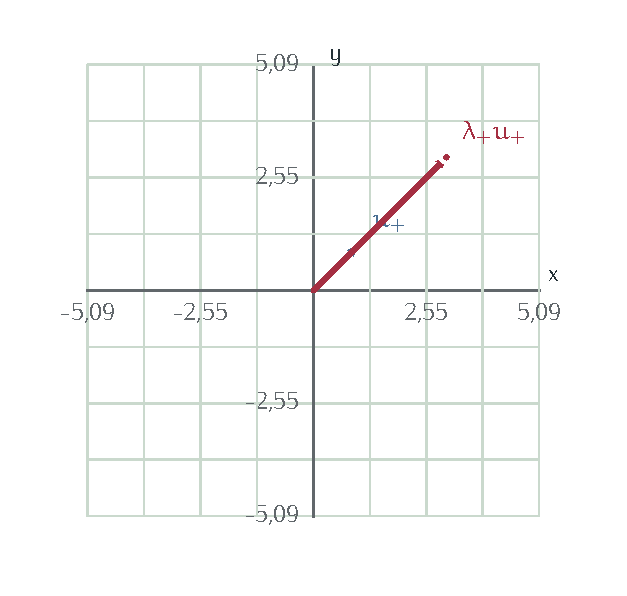
\includegraphics[width=\linewidth,height=94mm,keepaspectratio]{figure/f145b7ece3d8bfdfc.pdf}\FigureCaption{2.12 \(\cdot\) esempio 1 \(\cdot\) Prima autodirezione e sua immagine}\end{FigureBlock}
\begin{FigureBlock}\centering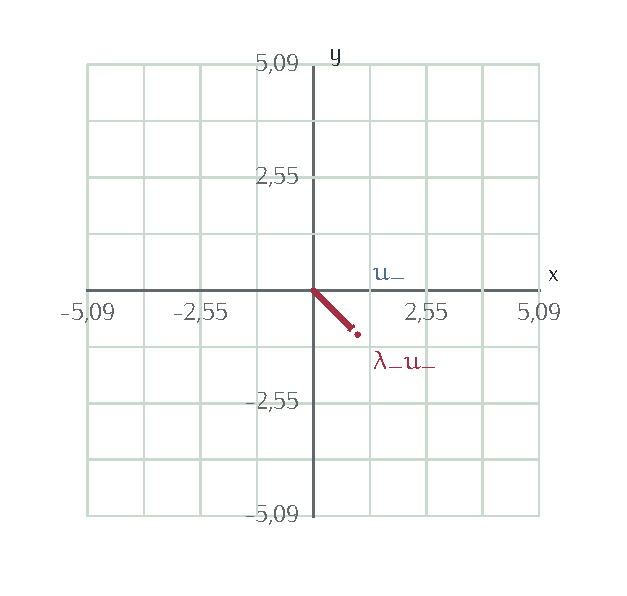
\includegraphics[width=\linewidth,height=94mm,keepaspectratio]{figure/fd27f35ef8e104b8a.pdf}\FigureCaption{2.12 \(\cdot\) esempio 1 \(\cdot\) Seconda autodirezione e sua immagine}\end{FigureBlock}

\phantomsection\label{c2-spettro-example-1-step-1}
\BookHeading{01 Imporre una soluzione non nulla}

\MathBlock{00640065007400280041221203BB00490029003D00280032221203BB002900B222120031003D0030}{\det (A- \lambda I)=(2- \lambda )^{2}- 1=0}
\MathBlock{0032221203BB003D00B10031002021D2002003BB208A003D0033002C002003BB208B003D0031}{2- \lambda =\pm 1\ \Rightarrow \ \lambda _{+}=3,\allowbreak \ \lambda _{-}=1}

L'annullamento del determinante rende singolare il sistema \((A- \lambda I)u=0\).\par


\phantomsection\label{c2-spettro-example-1-step-2}
\BookHeading{02 Risolvere i due sistemi}

\MathBlock{03BB208A003D0033003A002022120078002B0079003D0030002021D200200075208A003D00280031002C00310029}{\lambda _{+}=3:\ - x+y=0\ \Rightarrow \ u_{+}=(1{,}1)}
\MathBlock{03BB208B003D0031003A00200078002B0079003D0030002021D200200075208B003D00280031002C221200310029}{\lambda _{-}=1:\ x+y=0\ \Rightarrow \ u_{-}=(1,\allowbreak - 1)}

Sono scelte rappresentative delle due rette di soluzioni; nessun proiettore è necessario per riconoscerle.\par


\phantomsection\label{c2-spettro-example-1-step-3}
\BookHeading{03 Verificare le autodirezioni}

\MathBlock{00410075208A003D00280033002C00330029003D00330075208A}{Au_{+}=(3{,}3)=3u_{+}}
\MathBlock{00410075208B003D00280031002C002D00310029003D00310075208B}{Au_{-}=(1,\allowbreak -1)=1u_{-}}
\MathBlock{00410076003D00280035003B0020003400291D40}{Av=(5;\allowbreak \ 4)^{T}}

Il vettore generico v può cambiare direzione, mentre ciascun autovettore resta sulla propria retta.\par


\phantomsection\label{c2-spettro-example-1-step-4}
\BookHeading{04 Controllare che le direzioni siano distinte}

\MathBlock{27E80075208A002C0075208B27E9003D003100B70031002B003100B70028221200310029003D0030}{\langle u_{+},\allowbreak u_{-}\rangle =1\cdot 1+1\cdot (- 1)=0}
\MathBlock{006400650074005B005B0031002C0031005D002C005B0031002C22120031005D005D003D2212003122120031003D2212003222600030}{\det \begin{pmatrix}1&1\\1&- 1\end{pmatrix}=- 1- 1=- 2\ne 0}

I due vettori non nulli sono ortogonali e indipendenti. Potranno quindi essere normalizzati e usati come base nella sezione successiva.\par


\BookHeading{Interpretazione}

\(A\) moltiplica la direzione (1,1) per 3 e quella \((1,\allowbreak - 1)\) per 1. Queste due direzioni indipendenti permettono di ricostruire ogni ingresso.\par


\Needspace{.36\textheight}\phantomsection\label{c2-spettro-example-2}
{\sffamily\small\color{Accent} ESEMPIO SVOLTO 2\par}
\BookHeading{Autovalore negativo e inversione del verso}
Dati \(A=\)\(\begin{pmatrix}0&1\\1&0\end{pmatrix}\), \(v=(2{,}1)^{T}\).\par


\BookHeading{Geometria e configurazione dell'esempio}
\begin{FigureBlock}\centering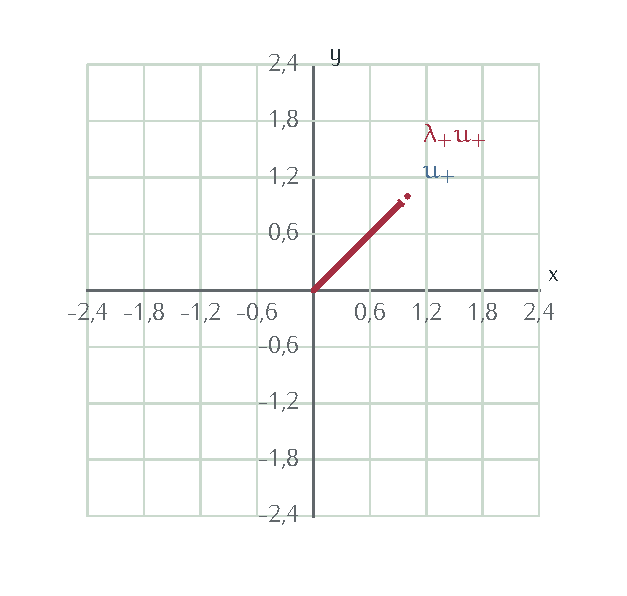
\includegraphics[width=\linewidth,height=94mm,keepaspectratio]{figure/f952f6960d029ddec.pdf}\FigureCaption{2.12 \(\cdot\) esempio 2 \(\cdot\) Prima autodirezione e sua immagine}\end{FigureBlock}
\begin{FigureBlock}\centering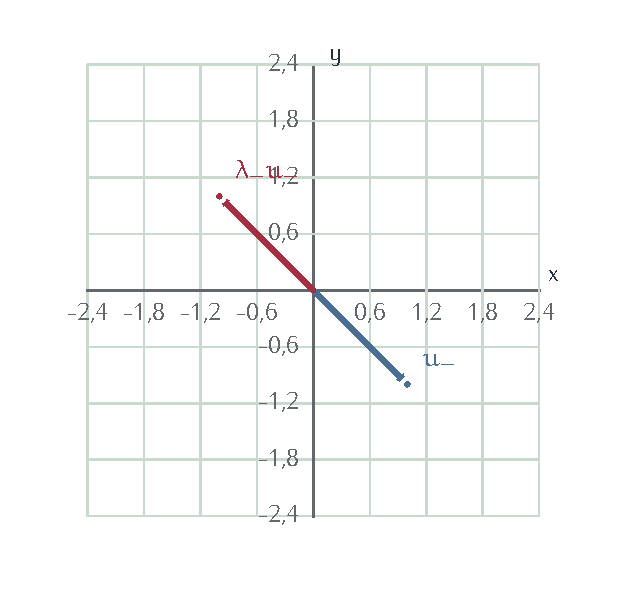
\includegraphics[width=\linewidth,height=94mm,keepaspectratio]{figure/ff631c8de28edf80b.pdf}\FigureCaption{2.12 \(\cdot\) esempio 2 \(\cdot\) Seconda autodirezione e sua immagine}\end{FigureBlock}

\phantomsection\label{c2-spettro-example-2-step-1}
\BookHeading{01 Imporre una soluzione non nulla}

\MathBlock{00640065007400280041221203BB00490029003D00280030221203BB002900B222120031003D0030}{\det (A- \lambda I)=(0- \lambda )^{2}- 1=0}
\MathBlock{0030221203BB003D00B10031002021D2002003BB208A003D0031002C002003BB208B003D002D0031}{0- \lambda =\pm 1\ \Rightarrow \ \lambda _{+}=1,\allowbreak \ \lambda _{-}=-1}

L'annullamento del determinante rende singolare il sistema \((A- \lambda I)u=0\).\par


\phantomsection\label{c2-spettro-example-2-step-2}
\BookHeading{02 Risolvere i due sistemi}

\MathBlock{03BB208A003D0031003A002022120078002B0079003D0030002021D200200075208A003D00280031002C00310029}{\lambda _{+}=1:\ - x+y=0\ \Rightarrow \ u_{+}=(1{,}1)}
\MathBlock{03BB208B003D002D0031003A00200078002B0079003D0030002021D200200075208B003D00280031002C221200310029}{\lambda _{-}=-1:\ x+y=0\ \Rightarrow \ u_{-}=(1,\allowbreak - 1)}

Sono scelte rappresentative delle due rette di soluzioni; nessun proiettore è necessario per riconoscerle.\par


\phantomsection\label{c2-spettro-example-2-step-3}
\BookHeading{03 Verificare le autodirezioni}

\MathBlock{00410075208A003D00280031002C00310029003D00310075208A}{Au_{+}=(1{,}1)=1u_{+}}
\MathBlock{00410075208B003D0028002D0031002C00310029003D002D00310075208B}{Au_{-}=(-1{,}1)=-1u_{-}}
\MathBlock{00410076003D00280031003B0020003200291D40}{Av=(1;\allowbreak \ 2)^{T}}

Il vettore generico v può cambiare direzione, mentre ciascun autovettore resta sulla propria retta.\par


\phantomsection\label{c2-spettro-example-2-step-4}
\BookHeading{04 Controllare che le direzioni siano distinte}

\MathBlock{27E80075208A002C0075208B27E9003D003100B70031002B003100B70028221200310029003D0030}{\langle u_{+},\allowbreak u_{-}\rangle =1\cdot 1+1\cdot (- 1)=0}
\MathBlock{006400650074005B005B0031002C0031005D002C005B0031002C22120031005D005D003D2212003122120031003D2212003222600030}{\det \begin{pmatrix}1&1\\1&- 1\end{pmatrix}=- 1- 1=- 2\ne 0}

I due vettori non nulli sono ortogonali e indipendenti. Potranno quindi essere normalizzati e usati come base nella sezione successiva.\par


\BookHeading{Interpretazione}

Gli autovalori +1 e \(- 1\) conservano le due rette; il secondo inverte il verso. Il vettore nullo non serve a individuare un'autodirezione.\par


\Needspace{7\baselineskip}
\BookHeading{Il passaggio successivo}
Le rette proprie possono diventare assi di coordinate. Normalizzeremo gli autovettori e ricostruiremo un ingresso mediante le sue componenti proprie.\par


\Needspace{.43\textheight}
\section{Costruire una base di autovettori}
\phantomsection\label{c2-base-propria}

{\sffamily\small\color{Ink!70} Riferimento alle slide: p. 113.\par}

{\sffamily\small\color{Ink!70} Laboratorio locale: \nolinkurl{index.html#capitolo-2/base-propria}\par}

\BookHeading{Definizioni e costruzione}
Dopo gli autovalori risolviamo i sistemi omogenei e normalizziamo le soluzioni. Le coordinate nella base propria separano i contributi.\par

Dopo aver trovato un autovalore, si risolve il corrispondente sistema omogeneo. Una componente può essere scelta liberamente; le altre vengono ricavate dalle equazioni. La soluzione viene poi divisa per la propria norma.\par

Per una matrice hermitiana è possibile scegliere una base ortonormale di autovettori. Le coordinate di v in quella base sono i prodotti interni \(\langle u_{j},\allowbreak v\rangle \). In presenza di un autovalore degenere, le equazioni individuano un intero autospazio, all'interno del quale si può scegliere una base ortonormale.\par


\MathBlock{0076003D03A32C7C27E800752C7C002C007627E900752C7C002000700065007200200075006E0061002000620061007300650020006F00720074006F006E006F0072006D0061006C00650020007B00752C7C007D002E}{v=\sum _{j}\langle u_{j},\allowbreak v\rangle u_{j}\ \text{per}\ \text{una}\ \text{base}\ \text{ortonormale}\ \{u_{j}\}.}

\BookHeading{Come leggere le figure}
Autovettori reali ortogonali; i coefficienti sono proiezioni.\par


\Needspace{.36\textheight}\phantomsection\label{c2-base-propria-example-1}
{\sffamily\small\color{Accent} ESEMPIO SVOLTO 1\par}
\BookHeading{Coordinate lungo gli autovettori}
Dati \(A=\)\(\begin{pmatrix}2&1\\1&2\end{pmatrix}\), \(v=(2{,}1)^{T}\). Caso progressivo della famiglia \(A=aI+\)\(\begin{pmatrix}0&1\\1&0\end{pmatrix}\), qui \(a=2\): riprendiamo le autodirezioni (1,1) e \((1,\allowbreak - 1)\) e svolgiamo il cambio di coordinate.\par


\BookHeading{Geometria e configurazione dell'esempio}
\begin{FigureBlock}\centering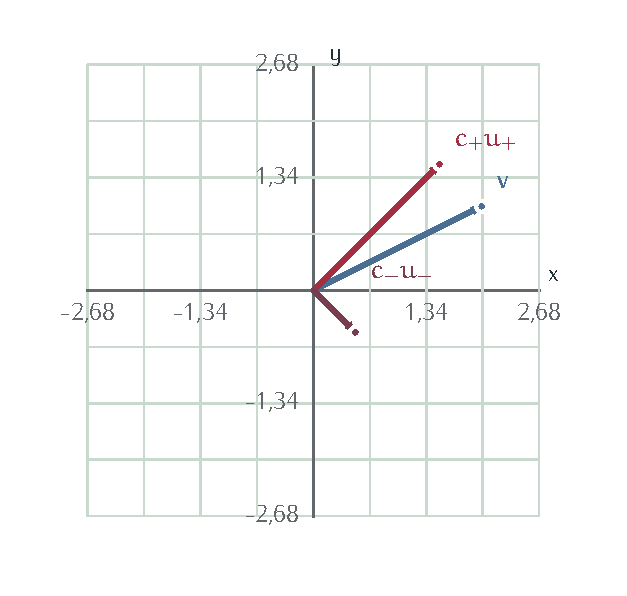
\includegraphics[width=\linewidth,height=94mm,keepaspectratio]{figure/f7c30847418be5ff6.pdf}\FigureCaption{2.13 \(\cdot\) esempio 1 \(\cdot\) Componenti nella base ortonormale}\end{FigureBlock}

\phantomsection\label{c2-base-propria-example-1-step-1}
\BookHeading{01 Normalizzare le autodirezioni}

\MathBlock{201600280031002C00B100310029201600B2003D0032003B00200075208A003D00280031002C00310029002F221A0032003B00200075208B003D00280031002C221200310029002F221A0032}{\Vert (1,\allowbreak \pm 1)\Vert ^{2}=2;\allowbreak \ u_{+}=(1{,}1)/\sqrt{2};\allowbreak \ u_{-}=(1,\allowbreak - 1)/\sqrt{2}}
\MathBlock{27E80075208A002C0075208B27E9003D00280031221200310029002F0032003D0030}{\langle u_{+},\allowbreak u_{-}\rangle =(1- 1)/2=0}

Le due soluzioni normalizzate formano una base ortonormale.\par


\phantomsection\label{c2-base-propria-example-1-step-2}
\BookHeading{02 Ottenere le coordinate proprie}

\MathBlock{0063208A003D27E80075208A002C007627E9003D00280032002B00310029002F221A0032003D0033002F221A0032}{c_{+}=\langle u_{+},\allowbreak v\rangle =(2+1)/\sqrt{2}=3/\sqrt{2}}
\MathBlock{0063208B003D27E80075208B002C007627E9003D00280032221200310029002F221A0032003D0031002F221A0032}{c_{-}=\langle u_{-},\allowbreak v\rangle =(2- 1)/\sqrt{2}=1/\sqrt{2}}

Le coordinate si ottengono dai prodotti interni grazie all'ortonormalità.\par


\phantomsection\label{c2-base-propria-example-1-step-3}
\BookHeading{03 Ricostruire il vettore}

\MathBlock{0063208A0075208A003D00280033002F0032002C0033002F00320029003B00200063208B0075208B003D00280031002F0032002C22120031002F00320029}{c_{+}u_{+}=(3/2{,}3/2);\allowbreak \ c_{-}u_{-}=(1/2,\allowbreak - 1/2)}
\MathBlock{0076003D0063208A0075208A002B0063208B0075208B003D00280032002C00310029}{v=c_{+}u_{+}+c_{-}u_{-}=(2{,}1)}

Le due componenti sono vettori del piano; i coefficienti sono numeri riferiti ai nuovi assi.\par


\phantomsection\label{c2-base-propria-example-1-step-4}
\BookHeading{04 Descrivere \(A\) nella base propria}

\MathBlock{0055003D005B0075208A00200075208B005D003B0020005520200055003D0049003B00200055202000410055003D006400690061006700280033002C00310029}{U=[u_{+}\ u_{-}];\allowbreak \ U{}^{\dagger} U=I;\allowbreak \ U{}^{\dagger} AU=\operatorname{diag}(3{,}1)}
\MathBlock{005B00410076005D0055003D0028003300B70033002F221A0032002C003100B70031002F221A003200291D40}{[Av]U=(3\cdot 3/\sqrt{2},\allowbreak 1\cdot 1/\sqrt{2})^{T}}

L'azione diventa diagonale perché ogni colonna è un autovettore.\par


\BookHeading{Interpretazione}

Le coordinate di v sono \((3/\sqrt{2},\allowbreak 1/\sqrt{2})\), mentre quelle di Av sono \((3\cdot 3/\sqrt{2},\allowbreak 1\cdot 1/\sqrt{2})\). La base dipende dalle direzioni; gli autovalori determinano i fattori applicati.\par


\Needspace{.36\textheight}\phantomsection\label{c2-base-propria-example-2}
{\sffamily\small\color{Accent} ESEMPIO SVOLTO 2\par}
\BookHeading{Stesse direzioni, autovalori traslati}
Dati \(A=\)\(\begin{pmatrix}3&1\\1&3\end{pmatrix}\), \(v=(2{,}1)^{T}\). Caso progressivo della famiglia \(A=aI+\)\(\begin{pmatrix}0&1\\1&0\end{pmatrix}\), qui \(a=3\): riprendiamo le autodirezioni (1,1) e \((1,\allowbreak - 1)\) e svolgiamo il cambio di coordinate.\par


\BookHeading{Geometria e configurazione dell'esempio}
\begin{FigureBlock}\centering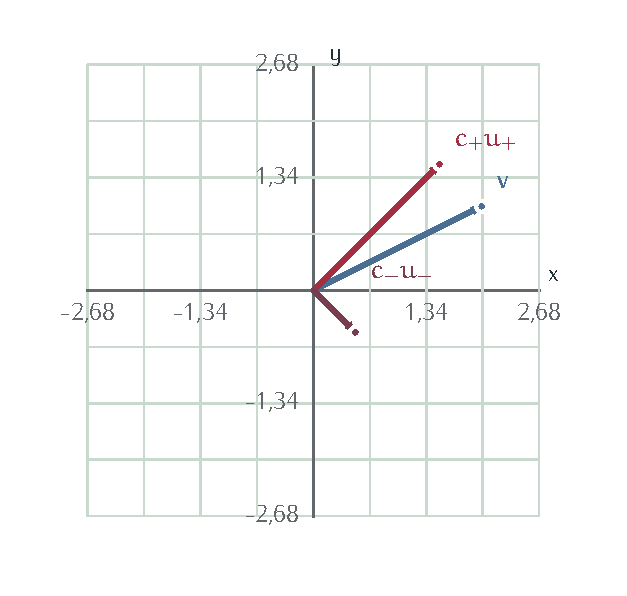
\includegraphics[width=\linewidth,height=94mm,keepaspectratio]{figure/feb319f4adad65fc4.pdf}\FigureCaption{2.13 \(\cdot\) esempio 2 \(\cdot\) Componenti nella base ortonormale}\end{FigureBlock}

\phantomsection\label{c2-base-propria-example-2-step-1}
\BookHeading{01 Normalizzare le autodirezioni}

\MathBlock{201600280031002C00B100310029201600B2003D0032003B00200075208A003D00280031002C00310029002F221A0032003B00200075208B003D00280031002C221200310029002F221A0032}{\Vert (1,\allowbreak \pm 1)\Vert ^{2}=2;\allowbreak \ u_{+}=(1{,}1)/\sqrt{2};\allowbreak \ u_{-}=(1,\allowbreak - 1)/\sqrt{2}}
\MathBlock{27E80075208A002C0075208B27E9003D00280031221200310029002F0032003D0030}{\langle u_{+},\allowbreak u_{-}\rangle =(1- 1)/2=0}

Le due soluzioni normalizzate formano una base ortonormale.\par


\phantomsection\label{c2-base-propria-example-2-step-2}
\BookHeading{02 Ottenere le coordinate proprie}

\MathBlock{0063208A003D27E80075208A002C007627E9003D00280032002B00310029002F221A0032003D0033002F221A0032}{c_{+}=\langle u_{+},\allowbreak v\rangle =(2+1)/\sqrt{2}=3/\sqrt{2}}
\MathBlock{0063208B003D27E80075208B002C007627E9003D00280032221200310029002F221A0032003D0031002F221A0032}{c_{-}=\langle u_{-},\allowbreak v\rangle =(2- 1)/\sqrt{2}=1/\sqrt{2}}

Le coordinate si ottengono dai prodotti interni grazie all'ortonormalità.\par


\phantomsection\label{c2-base-propria-example-2-step-3}
\BookHeading{03 Ricostruire il vettore}

\MathBlock{0063208A0075208A003D00280033002F0032002C0033002F00320029003B00200063208B0075208B003D00280031002F0032002C22120031002F00320029}{c_{+}u_{+}=(3/2{,}3/2);\allowbreak \ c_{-}u_{-}=(1/2,\allowbreak - 1/2)}
\MathBlock{0076003D0063208A0075208A002B0063208B0075208B003D00280032002C00310029}{v=c_{+}u_{+}+c_{-}u_{-}=(2{,}1)}

Le due componenti sono vettori del piano; i coefficienti sono numeri riferiti ai nuovi assi.\par


\phantomsection\label{c2-base-propria-example-2-step-4}
\BookHeading{04 Descrivere \(A\) nella base propria}

\MathBlock{0055003D005B0075208A00200075208B005D003B0020005520200055003D0049003B00200055202000410055003D006400690061006700280034002C00320029}{U=[u_{+}\ u_{-}];\allowbreak \ U{}^{\dagger} U=I;\allowbreak \ U{}^{\dagger} AU=\operatorname{diag}(4{,}2)}
\MathBlock{005B00410076005D0055003D0028003400B70033002F221A0032002C003200B70031002F221A003200291D40}{[Av]U=(4\cdot 3/\sqrt{2},\allowbreak 2\cdot 1/\sqrt{2})^{T}}

L'azione diventa diagonale perché ogni colonna è un autovettore.\par


\BookHeading{Interpretazione}

Le coordinate di v sono \((3/\sqrt{2},\allowbreak 1/\sqrt{2})\), mentre quelle di Av sono \((4\cdot 3/\sqrt{2},\allowbreak 2\cdot 1/\sqrt{2})\). La base dipende dalle direzioni; gli autovalori determinano i fattori applicati.\par


\Needspace{7\baselineskip}
\BookHeading{Il passaggio successivo}
I coefficienti propri ricostruiscono il vettore. I prodotti esterni degli assi unitari permetteranno di calcolare ogni componente mediante una matrice proiettore.\par


\Needspace{.43\textheight}
\section{Separare e ricomporre le componenti}
\phantomsection\label{c2-proiettori}

{\sffamily\small\color{Ink!70} Riferimento alle slide: p. 113.\par}

{\sffamily\small\color{Ink!70} Laboratorio locale: \nolinkurl{index.html#capitolo-2/proiettori}\par}

\BookHeading{Definizioni e costruzione}
Il proiettore conserva la componente lungo una direzione unitaria. La somma dei proiettori di una base completa restituisce il vettore iniziale.\par

Per una direzione unitaria u, il prodotto esterno \(uu{}^{\dagger} \) è una matrice. Applicandola a v si ottiene \(u(u{}^{\dagger} v)\), ossia il vettore lungo u con il coefficiente di proiezione corretto. Il risultato resta invariato se si applica nuovamente lo stesso proiettore.\par

Proiettori su direzioni ortogonali hanno prodotto nullo. Quando le direzioni formano una base completa, la loro somma è l'identità e le componenti proiettate ricostruiscono il vettore iniziale. La successiva interpretazione come misura richiederà anche probabilità e rinormalizzazione del ramo selezionato.\par


\MathBlock{00502C7C003D00752C7C00752C7C2020003B002000502C7C00B2003D00502C7C003B002003A32C7C00502C7C003D0049002E}{P_{j}=u_{j}u_{j}{}^{\dagger} ;\allowbreak \ P_{j}^{2}=P_{j};\allowbreak \ \sum _{j}P_{j}=I.}

\BookHeading{Come leggere le figure}
Proiezioni nel piano reale; l'operazione modifica il vettore.\par


\Needspace{.36\textheight}\phantomsection\label{c2-proiettori-example-1}
{\sffamily\small\color{Accent} ESEMPIO SVOLTO 1\par}
\BookHeading{Proiettori come matrici}
Dati \(A=\)\(\begin{pmatrix}2&1\\1&2\end{pmatrix}\), \(v=(2{,}1)^{T}\). Caso progressivo della famiglia \(A=aI+\)\(\begin{pmatrix}0&1\\1&0\end{pmatrix}\), qui \(a=2\): riprendiamo le autodirezioni (1,1) e \((1,\allowbreak - 1)\) e svolgiamo la costruzione dei proiettori. Qui \(w=v\).\par


\BookHeading{Geometria e configurazione dell'esempio}
\begin{FigureBlock}\centering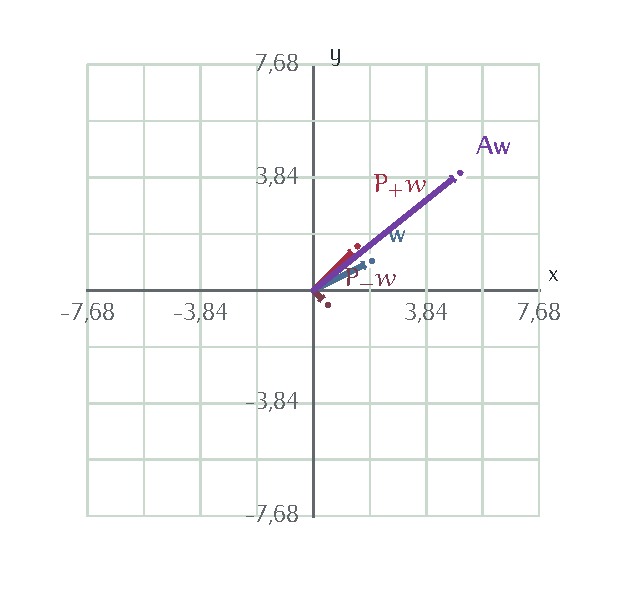
\includegraphics[width=\linewidth,height=94mm,keepaspectratio]{figure/f128a32ba94aa3b58.pdf}\FigureCaption{2.14 \(\cdot\) esempio 1 \(\cdot\) Vettore e proiezioni complementari}\end{FigureBlock}

\phantomsection\label{c2-proiettori-example-1-step-1}
\BookHeading{01 Formare i prodotti esterni}

\MathBlock{0050208A003D0075208A0075208A2020003D00280031002F00320029005B005B0031002C0031005D002C005B0031002C0031005D005D}{P_{+}=u_{+}u_{+}{}^{\dagger} =(1/2)\begin{pmatrix}1&1\\1&1\end{pmatrix}}
\MathBlock{0050208B003D0075208B0075208B2020003D00280031002F00320029005B005B0031002C22120031005D002C005B22120031002C0031005D005D}{P_{-}=u_{-}u_{-}{}^{\dagger} =(1/2)\begin{pmatrix}1&- 1\\- 1&1\end{pmatrix}}

Moltiplicare una colonna per una riga produce i quattro elementi di ciascuna matrice.\par


\phantomsection\label{c2-proiettori-example-1-step-2}
\BookHeading{02 Applicare i due operatori}

\MathBlock{00500065007200200077003D00280032003B0020003100291D40003A}{\text{Per}\ w=(2;\allowbreak \ 1)^{T}:}
\MathBlock{0050208A0077003D00280032002B00310029002F003200B700280031002C00310029003D00280031002C0035003B00200031002C003500291D40}{P_{+}w=(2+1)/2\cdot (1{,}1)=(1{,}5;\allowbreak \ 1{,}5)^{T}}
\MathBlock{0050208B0077003D0028003222120028003100290029002F003200B700280031002C221200310029003D00280030002C0035003B0020002D0030002C003500291D40}{P_{-}w=(2- (1))/2\cdot (1,\allowbreak - 1)=(0{,}5;\allowbreak \ -0{,}5)^{T}}

Ogni proiettore mantiene soltanto il contributo sulla propria direzione.\par


\phantomsection\label{c2-proiettori-example-1-step-3}
\BookHeading{03 Verificare le proprietà}

\MathBlock{0050208A00B2003D00280031002F00340029005B005B0032002C0032005D002C005B0032002C0032005D005D003D0050208A003B00200050208B00B2003D0050208B}{P_{+}^{2}=(1/4)\begin{pmatrix}2&2\\2&2\end{pmatrix}=P_{+};\allowbreak \ P_{-}^{2}=P_{-}}
\MathBlock{0050208A0050208B003D00280031002F00340029005B005B0030002C0030005D002C005B0030002C0030005D005D003D0030003B00200050208A002B0050208B003D0049}{P_{+}P_{-}=(1/4)\begin{pmatrix}0&0\\0&0\end{pmatrix}=0;\allowbreak \ P_{+}+P_{-}=I}

Una componente già proiettata resta uguale; direzioni ortogonali si eliminano reciprocamente.\par


\phantomsection\label{c2-proiettori-example-1-step-4}
\BookHeading{04 Ricomporre \(A\) e la sua azione}

\MathBlock{0041003D00330050208A002B00310050208B}{A=3P_{+}+1P_{-}}
\MathBlock{00410077003D00330050208A0077002B00310050208B0077003D00280035003B0020003400291D40}{Aw=3P_{+}w+1P_{-}w=(5;\allowbreak \ 4)^{T}}

La somma dei proiettori pesati dagli autovalori ricostruisce l'operatore originale.\par


\BookHeading{Interpretazione}

I proiettori separano (2,1) in (3/2,3/2) e \((1/2,\allowbreak - 1/2)\). Pesare queste parti con 3 e 1 produce \(Av=(5{,}4)\).\par


\Needspace{.36\textheight}\phantomsection\label{c2-proiettori-example-2}
{\sffamily\small\color{Accent} ESEMPIO SVOLTO 2\par}
\BookHeading{Proiezione nulla su una direzione ortogonale}
Dati \(A=\)\(\begin{pmatrix}3&1\\1&3\end{pmatrix}\), \(v=(2{,}1)^{T}\). Caso progressivo della famiglia \(A=aI+\)\(\begin{pmatrix}0&1\\1&0\end{pmatrix}\), qui \(a=3\): riprendiamo le autodirezioni (1,1) e \((1,\allowbreak - 1)\) e svolgiamo la costruzione dei proiettori. Per evidenziare un ramo nullo scegliamo come ingresso \(w=(1,\allowbreak - 1)\).\par


\BookHeading{Geometria e configurazione dell'esempio}
\begin{FigureBlock}\centering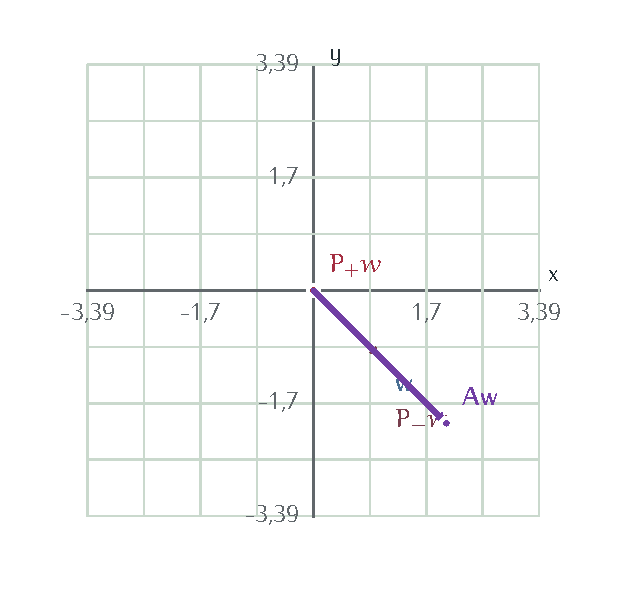
\includegraphics[width=\linewidth,height=94mm,keepaspectratio]{figure/f0978ed2d2275afe2.pdf}\FigureCaption{2.14 \(\cdot\) esempio 2 \(\cdot\) Vettore e proiezioni complementari}\end{FigureBlock}

\phantomsection\label{c2-proiettori-example-2-step-1}
\BookHeading{01 Formare i prodotti esterni}

\MathBlock{0050208A003D0075208A0075208A2020003D00280031002F00320029005B005B0031002C0031005D002C005B0031002C0031005D005D}{P_{+}=u_{+}u_{+}{}^{\dagger} =(1/2)\begin{pmatrix}1&1\\1&1\end{pmatrix}}
\MathBlock{0050208B003D0075208B0075208B2020003D00280031002F00320029005B005B0031002C22120031005D002C005B22120031002C0031005D005D}{P_{-}=u_{-}u_{-}{}^{\dagger} =(1/2)\begin{pmatrix}1&- 1\\- 1&1\end{pmatrix}}

Moltiplicare una colonna per una riga produce i quattro elementi di ciascuna matrice.\par


\phantomsection\label{c2-proiettori-example-2-step-2}
\BookHeading{02 Applicare i due operatori}

\MathBlock{00500065007200200077003D00280031003B0020002D003100291D40003A}{\text{Per}\ w=(1;\allowbreak \ -1)^{T}:}
\MathBlock{0050208A0077003D00280031002B002D00310029002F003200B700280031002C00310029003D00280030003B0020003000291D40}{P_{+}w=(1+-1)/2\cdot (1{,}1)=(0;\allowbreak \ 0)^{T}}
\MathBlock{0050208B0077003D0028003122120028002D003100290029002F003200B700280031002C221200310029003D00280031003B0020002D003100291D40}{P_{-}w=(1- (-1))/2\cdot (1,\allowbreak - 1)=(1;\allowbreak \ -1)^{T}}

Ogni proiettore mantiene soltanto il contributo sulla propria direzione.\par


\phantomsection\label{c2-proiettori-example-2-step-3}
\BookHeading{03 Verificare le proprietà}

\MathBlock{0050208A00B2003D00280031002F00340029005B005B0032002C0032005D002C005B0032002C0032005D005D003D0050208A003B00200050208B00B2003D0050208B}{P_{+}^{2}=(1/4)\begin{pmatrix}2&2\\2&2\end{pmatrix}=P_{+};\allowbreak \ P_{-}^{2}=P_{-}}
\MathBlock{0050208A0050208B003D00280031002F00340029005B005B0030002C0030005D002C005B0030002C0030005D005D003D0030003B00200050208A002B0050208B003D0049}{P_{+}P_{-}=(1/4)\begin{pmatrix}0&0\\0&0\end{pmatrix}=0;\allowbreak \ P_{+}+P_{-}=I}

Una componente già proiettata resta uguale; direzioni ortogonali si eliminano reciprocamente.\par


\phantomsection\label{c2-proiettori-example-2-step-4}
\BookHeading{04 Ricomporre \(A\) e la sua azione}

\MathBlock{0041003D00340050208A002B00320050208B}{A=4P_{+}+2P_{-}}
\MathBlock{00410077003D00340050208A0077002B00320050208B0077003D00280032003B0020002D003200291D40}{Aw=4P_{+}w+2P_{-}w=(2;\allowbreak \ -2)^{T}}

La somma dei proiettori pesati dagli autovalori ricostruisce l'operatore originale.\par


\BookHeading{Interpretazione}

\(P_{+}w=0\) perché w è ortogonale a \(u_{+}\); \(P_{-}w=w\). La somma dei due operatori conserva comunque ogni vettore.\par


\Needspace{7\baselineskip}
\BookHeading{Il passaggio successivo}
La somma dei proiettori pesati dagli autovalori ricostruisce \(A\). Sostituire una funzione agli autovalori permetterà di ottenere potenze ed esponenziali.\par


\Needspace{.43\textheight}
\section{Calcolare con la decomposizione spettrale}
\phantomsection\label{c2-funzioni-matrice}

{\sffamily\small\color{Ink!70} Riferimento alle slide: p. 180.\par}

{\sffamily\small\color{Ink!70} Laboratorio locale: \nolinkurl{index.html#capitolo-2/funzioni-matrice}\par}

\BookHeading{Definizioni e costruzione}
Nella base propria una funzione della matrice agisce separatamente su ciascun autovalore. Possiamo poi ricostruire il risultato nella base iniziale.\par

La decomposizione spettrale \(A=\sum _{j}\lambda _{j}P_{j}\) separa i sottospazi sui quali la matrice agisce con un semplice fattore. Poiché \(P_{j}P_{k}=0\) per \(j\ne k\) e \(P_{j}^{2}=P_{j}\), il prodotto di due decomposizioni dà \(A^{2}=\sum _{j}\lambda _{j}^{2}P_{j}\). Ripetendo il prodotto si ottiene \(A^{n}=\sum _{j}\lambda _{j}^{n}P_{j}\), con \(A^{0}=I\).\par

Si definisce \(f(A)=\sum _{j}f(\lambda _{j})P_{j}\). Per l'esponenziale la definizione coincide con la serie \(e^{- \text{itA}}=\sum _{n=0}\infty (- it)^{n}A^{n}/n!\): inserendo la formula per \(A^{n}\) si riconosce, su ciascun autospazio, la serie scalare \(e^{- it\lambda _{j}}\). Per una matrice hermitiana gli autovalori sono reali e questi fattori hanno modulo uno; \(U{}^{\dagger} U=\sum _{j}|e^{- it\lambda _{j}}|^{2}P_{j}=I\).\par

I due esempi conservano la famiglia di matrici già diagonalizzata e aggiungono operazioni nuove: il quadrato moltiplica le componenti proprie per gli autovalori al quadrato, mentre l'esponenziale ne ruota le fasi. Qui t è un parametro adimensionale. Nel modulo 3 questa famiglia di operatori diventerà un modello di evoluzione con un generatore dichiarato. In caso degenere si usa un proiettore per l'intero autospazio: per \(A=2I\), \(f(A)=f(2)I\).\par


\MathBlock{0041003D03A32C7C03BB2C7C00502C7C003B00200066002800410029003D03A32C7C0066002803BB2C7C002900502C7C002E}{A=\sum _{j}\lambda _{j}P_{j};\allowbreak \ f(A)=\sum _{j}f(\lambda _{j})P_{j}.}

\BookHeading{Come leggere le figure}
Direzioni proprie e fattori di scala; le potenze conservano gli autovettori.\par


\Needspace{.36\textheight}\phantomsection\label{c2-funzioni-matrice-example-1}
{\sffamily\small\color{Accent} ESEMPIO SVOLTO 1\par}
\BookHeading{Quadrato ed esponenziale spettrale}
Dati \(A=\)\(\begin{pmatrix}2&1\\1&2\end{pmatrix}\), \(v=(2{,}1)^{T}\). Caso progressivo della famiglia \(A=aI+\)\(\begin{pmatrix}0&1\\1&0\end{pmatrix}\), qui \(a=2\): riprendiamo le autodirezioni (1,1) e \((1,\allowbreak - 1)\) e svolgiamo le funzioni della matrice.\par


\BookHeading{Geometria e configurazione dell'esempio}
\begin{FigureBlock}\centering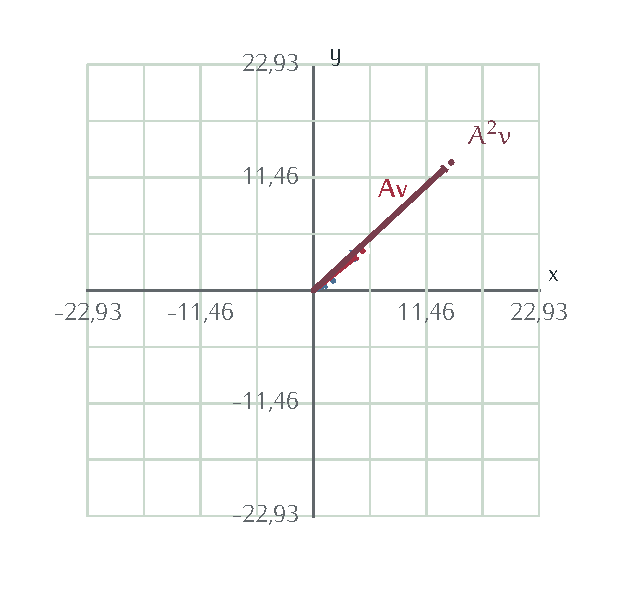
\includegraphics[width=\linewidth,height=94mm,keepaspectratio]{figure/fb90f94e67eb0707e.pdf}\FigureCaption{2.15 \(\cdot\) esempio 1 \(\cdot\) Potenze: v, Av e \(A^{2}v\) sulla stessa scala}\end{FigureBlock}
\begin{FigureBlock}\begin{minipage}[t]{.485\linewidth}\centering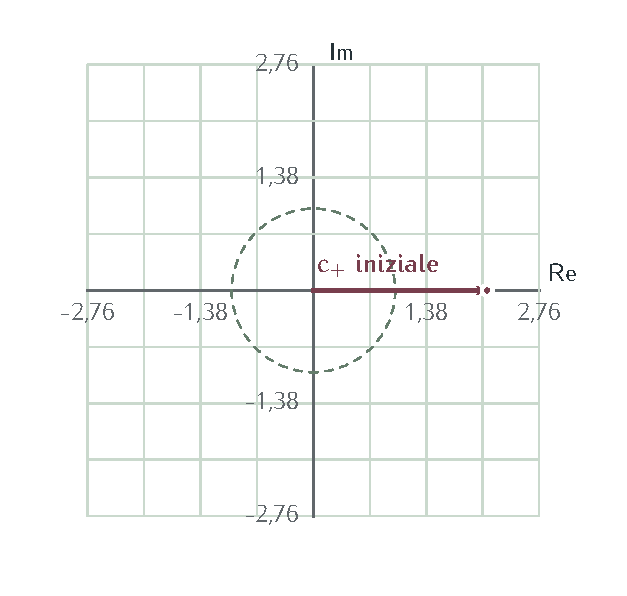
\includegraphics[width=\linewidth,height=63mm,keepaspectratio]{figure/f5063e83deff6f0c4.pdf}\par{\sffamily\footnotesize \(c_{+}\) iniziale\par}\end{minipage}\hfill\begin{minipage}[t]{.485\linewidth}\centering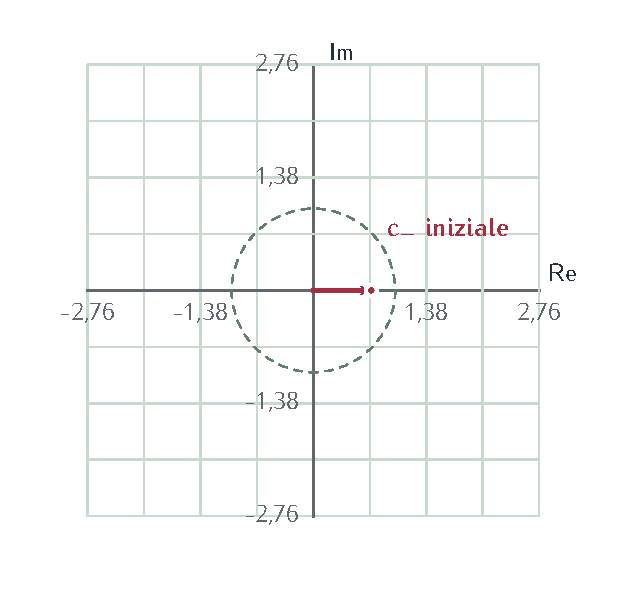
\includegraphics[width=\linewidth,height=63mm,keepaspectratio]{figure/f8758b53a512e921a.pdf}\par{\sffamily\footnotesize \(c_{-}\) iniziale\par}\end{minipage}\FigureCaption{2.15 \(\cdot\) esempio 1 \(\cdot\) Piano complesso: fasi sulle componenti proprie}\end{FigureBlock}
\begin{FigureBlock}\begin{minipage}[t]{.485\linewidth}\centering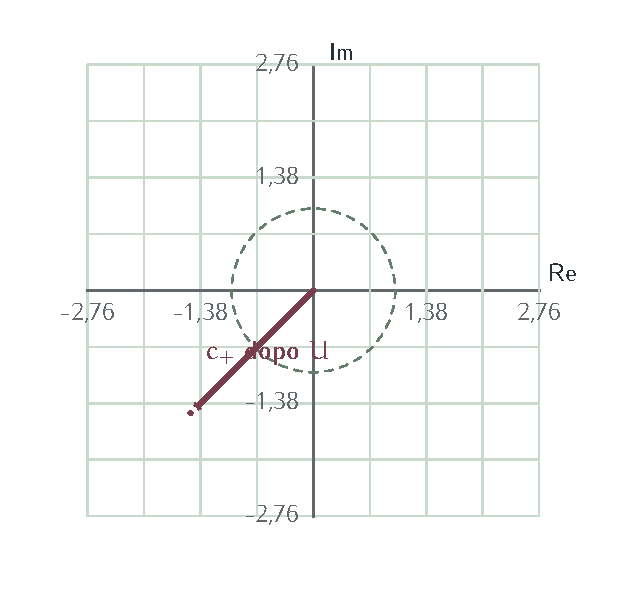
\includegraphics[width=\linewidth,height=63mm,keepaspectratio]{figure/fbcaff91246b7c8d3.pdf}\par{\sffamily\footnotesize \(c_{+}\) dopo \(U\)\par}\end{minipage}\hfill\begin{minipage}[t]{.485\linewidth}\centering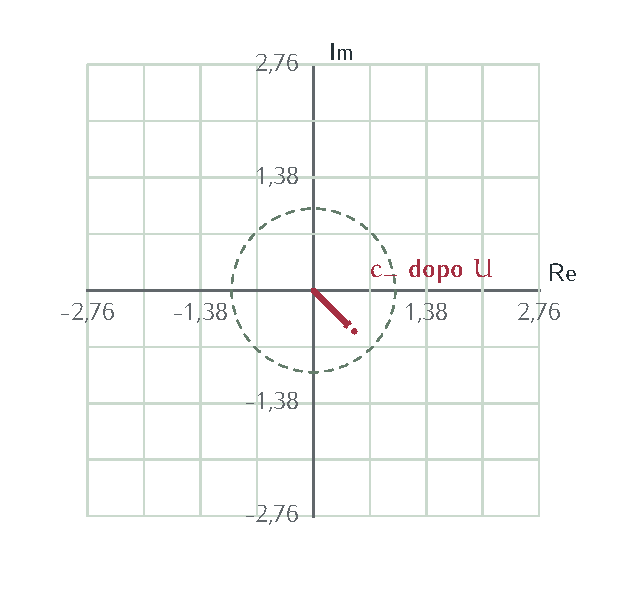
\includegraphics[width=\linewidth,height=63mm,keepaspectratio]{figure/fd86b897dc8763cd2.pdf}\par{\sffamily\footnotesize \(c_{-}\) dopo \(U\)\par}\end{minipage}\FigureCaption{2.15 \(\cdot\) esempio 1 \(\cdot\) Piano complesso: fasi sulle componenti proprie}\end{FigureBlock}
\begin{FigureBlock}\begin{minipage}[t]{.485\linewidth}\centering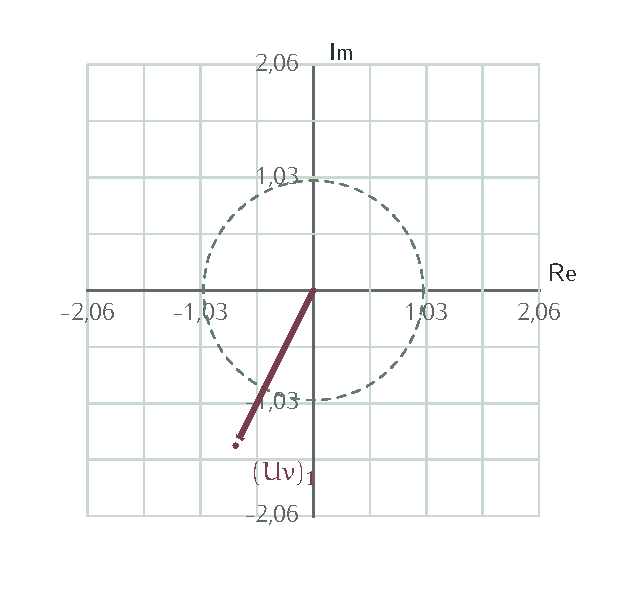
\includegraphics[width=\linewidth,height=63mm,keepaspectratio]{figure/f7a08bccd6c1e394b.pdf}\par{\sffamily\footnotesize \((Uv)_{1}\)\par}\end{minipage}\hfill\begin{minipage}[t]{.485\linewidth}\centering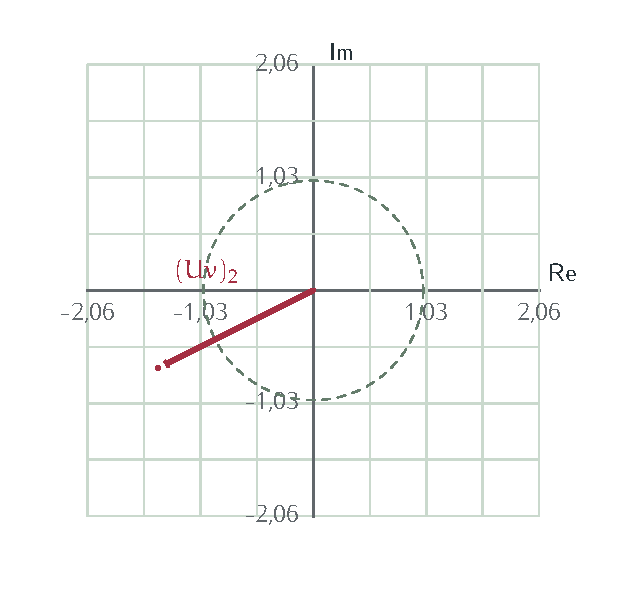
\includegraphics[width=\linewidth,height=63mm,keepaspectratio]{figure/f140d143ded858c56.pdf}\par{\sffamily\footnotesize \((Uv)_{2}\)\par}\end{minipage}\FigureCaption{2.15 \(\cdot\) esempio 1 \(\cdot\) Componenti canoniche dopo l'esponenziale}\end{FigureBlock}

\phantomsection\label{c2-funzioni-matrice-example-1-step-1}
\BookHeading{01 Richiamare la decomposizione già costruita}

\MathBlock{0050208A003D00280031002F00320029005B005B0031002C0031005D002C005B0031002C0031005D005D003B00200050208B003D00280031002F00320029005B005B0031002C22120031005D002C005B22120031002C0031005D005D}{P_{+}=(1/2)\begin{pmatrix}1&1\\1&1\end{pmatrix};\allowbreak \ P_{-}=(1/2)\begin{pmatrix}1&- 1\\- 1&1\end{pmatrix}}
\MathBlock{0041003D00330050208A002B00310050208B003B00200070003D0050208A0076003D00280033002F0032002C0033002F00320029003B00200071003D0050208B0076003D00280031002F0032002C22120031002F00320029}{A=3P_{+}+1P_{-};\allowbreak \ p=P_{+}v=(3/2{,}3/2);\allowbreak \ q=P_{-}v=(1/2,\allowbreak - 1/2)}

I proiettori sono quelli verificati nella sezione precedente; qui diventano strumenti per applicare una funzione.\par


\phantomsection\label{c2-funzioni-matrice-example-1-step-2}
\BookHeading{02 Moltiplicare due decomposizioni}

\MathBlock{004100B2003D002800330050208A002B00310050208B002900B2003D00390050208A002B00310050208B}{A^{2}=(3P_{+}+1P_{-})^{2}=9P_{+}+1P_{-}}
\MathBlock{00410076003D00280035003B0020003400291D40003B0020004100B20076003D00390070002B00310071003D002800310034003B00200031003300291D40}{Av=(5;\allowbreak \ 4)^{T};\allowbreak \ A^{2}v=9p+1q=(14;\allowbreak \ 13)^{T}}

I termini misti svaniscono perché \(P_{+}P_{-}=P_{-}P_{+}=0\); ogni \(P^{2}\) si riduce a \(P\).\par


\phantomsection\label{c2-funzioni-matrice-example-1-step-3}
\BookHeading{03 Definire e sommare l'esponenziale}

\MathBlock{0065005E002822120069007400410029003D03A32099208C2080221E00282212006900740029207F0041207F002F006E0021}{e^{- \text{itA}}=\sum _{n=0}\infty (- it)^{n}A^{n}/n!}
\MathBlock{003D03A32099002822120069007403BB208A0029207F0050208A002F006E0021002B03A32099002822120069007403BB208B0029207F0050208B002F006E0021}{=\sum _{n}(- it\lambda _{+})^{n}P_{+}/n!+\sum _{n}(- it\lambda _{-})^{n}P_{-}/n!}
\MathBlock{003D0065005E0028221200690033007400290050208A002B0065005E0028221200690031007400290050208B}{=e^{- i3t}P_{+}+e^{- i1t}P_{-}}

La serie scalare dell'esponenziale si applica separatamente ai due autovalori. Il parametro t è adimensionale in questo esempio algebrico.\par


\phantomsection\label{c2-funzioni-matrice-example-1-step-4}
\BookHeading{04 Sostituire un parametro preciso}

\MathBlock{0074003D03C0002F0034003A00200065005E002822120069003303C0002F00340029003D002822120031221200690029002F221A0032003B00200065005E00282212006903C0002F00340029003D00280031221200690029002F221A0032}{t=\pi /4:\ e^{- i3\pi /4}=(- 1- i)/\sqrt{2};\allowbreak \ e^{- i\pi /4}=(1- i)/\sqrt{2}}
\MathBlock{0055003D00280031002F221A00320029005B005B22120069002C22120031005D002C005B22120031002C22120069005D005D}{U=(1/\sqrt{2})\begin{pmatrix}- i&- 1\\- 1&- i\end{pmatrix}}
\MathBlock{00550076003D00280028221200312212003200690029002F221A0032002C002822120032221200690029002F221A003200291D40}{Uv=((- 1- 2i)/\sqrt{2},\allowbreak (- 2- i)/\sqrt{2})^{T}}

I fattori hanno modulo uno, quindi ruotano le componenti proprie senza cambiarne il peso.\par


\phantomsection\label{c2-funzioni-matrice-example-1-step-5}
\BookHeading{05 Verificare unitarietà e norma}

\MathBlock{005520200055003D007C0065005E002822120069007403BB208A0029007C00B20050208A002B007C0065005E002822120069007403BB208B0029007C00B20050208B003D0050208A002B0050208B003D0049}{U{}^{\dagger} U=|e^{- it\lambda _{+}}|^{2}P_{+}+|e^{- it\lambda _{-}}|^{2}P_{-}=P_{+}+P_{-}=I}
\MathBlock{201600550076201600B2003D20160076201600B2003D0035}{\Vert Uv\Vert ^{2}=\Vert v\Vert ^{2}=5}

L'esponenziale immaginario di una matrice hermitiana conserva la norma. Questa identità prepara il modello di evoluzione del modulo 3.\par


\BookHeading{Interpretazione}

Il quadrato produce \(A^{2}v=(14\); \(13)^{T}\), mentre \(e^{- \text{itA}}\) conserva la norma quadra 5. Le potenze amplificano i coefficienti propri; l'esponenziale qui svolto ne cambia le fasi.\par


\Needspace{.36\textheight}\phantomsection\label{c2-funzioni-matrice-example-2}
{\sffamily\small\color{Accent} ESEMPIO SVOLTO 2\par}
\BookHeading{Quadrato, scambio unitario e degenerazione}
Dati \(A=\)\(\begin{pmatrix}3&1\\1&3\end{pmatrix}\), \(v=(2{,}1)^{T}\). Caso progressivo della famiglia \(A=aI+\)\(\begin{pmatrix}0&1\\1&0\end{pmatrix}\), qui \(a=3\): riprendiamo le autodirezioni (1,1) e \((1,\allowbreak - 1)\) e svolgiamo le funzioni della matrice.\par


\BookHeading{Geometria e configurazione dell'esempio}
\begin{FigureBlock}\centering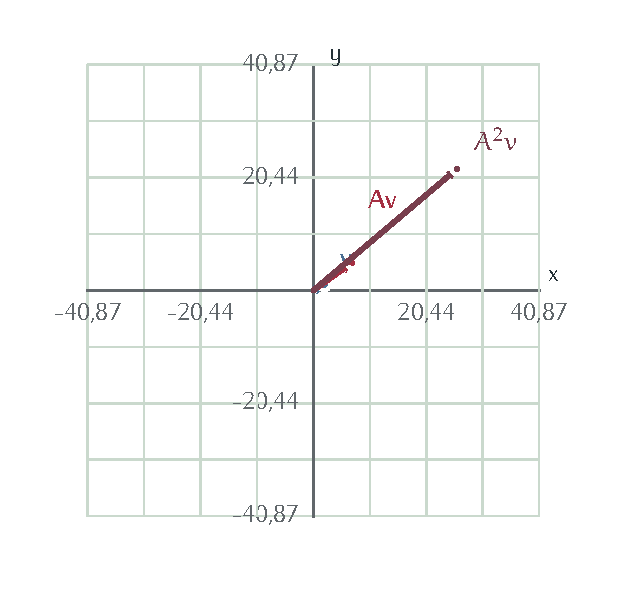
\includegraphics[width=\linewidth,height=94mm,keepaspectratio]{figure/f251f6fdd79fbb1dd.pdf}\FigureCaption{2.15 \(\cdot\) esempio 2 \(\cdot\) Potenze: v, Av e \(A^{2}v\) sulla stessa scala}\end{FigureBlock}
\begin{FigureBlock}\begin{minipage}[t]{.485\linewidth}\centering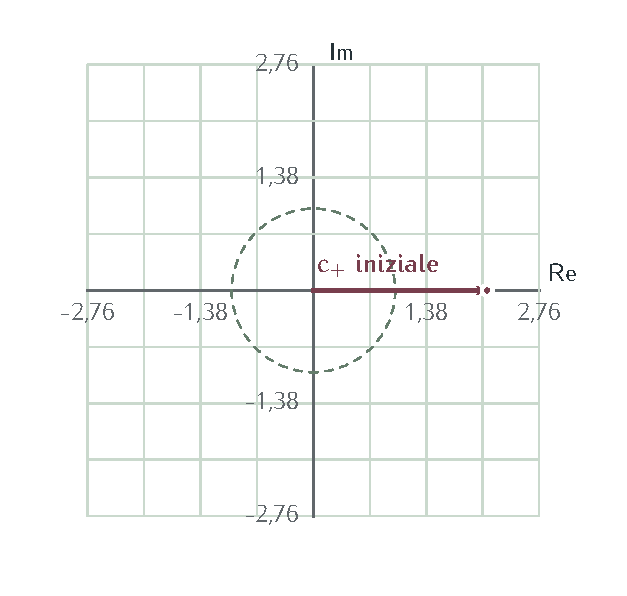
\includegraphics[width=\linewidth,height=63mm,keepaspectratio]{figure/fb953108751f3f230.pdf}\par{\sffamily\footnotesize \(c_{+}\) iniziale\par}\end{minipage}\hfill\begin{minipage}[t]{.485\linewidth}\centering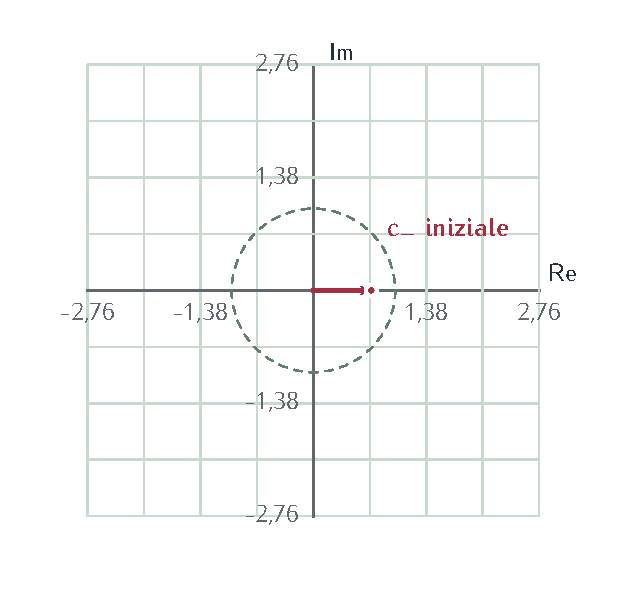
\includegraphics[width=\linewidth,height=63mm,keepaspectratio]{figure/ffbeb11cf0f31232b.pdf}\par{\sffamily\footnotesize \(c_{-}\) iniziale\par}\end{minipage}\FigureCaption{2.15 \(\cdot\) esempio 2 \(\cdot\) Piano complesso: fasi sulle componenti proprie}\end{FigureBlock}
\begin{FigureBlock}\begin{minipage}[t]{.485\linewidth}\centering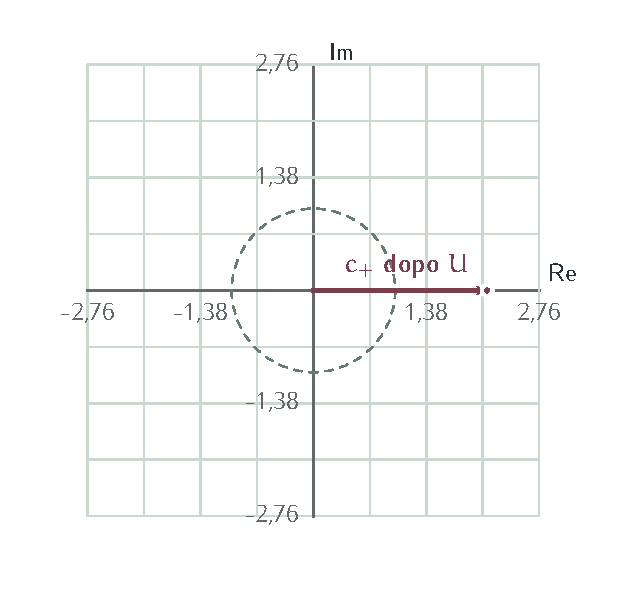
\includegraphics[width=\linewidth,height=63mm,keepaspectratio]{figure/f2a67c2078d38fa0a.pdf}\par{\sffamily\footnotesize \(c_{+}\) dopo \(U\)\par}\end{minipage}\hfill\begin{minipage}[t]{.485\linewidth}\centering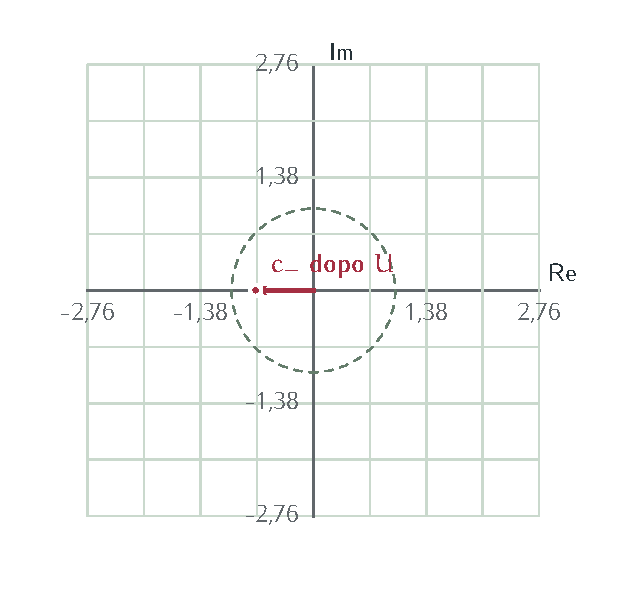
\includegraphics[width=\linewidth,height=63mm,keepaspectratio]{figure/fcc15508c75da8719.pdf}\par{\sffamily\footnotesize \(c_{-}\) dopo \(U\)\par}\end{minipage}\FigureCaption{2.15 \(\cdot\) esempio 2 \(\cdot\) Piano complesso: fasi sulle componenti proprie}\end{FigureBlock}
\begin{FigureBlock}\begin{minipage}[t]{.485\linewidth}\centering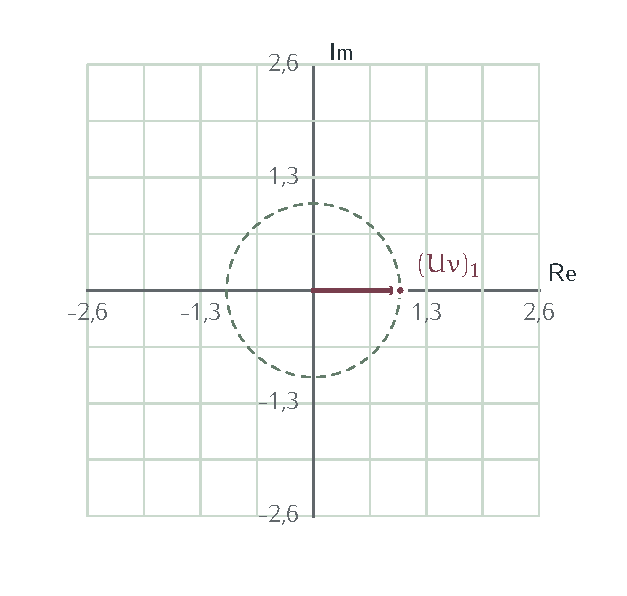
\includegraphics[width=\linewidth,height=63mm,keepaspectratio]{figure/f8ffc6616f4c51c05.pdf}\par{\sffamily\footnotesize \((Uv)_{1}\)\par}\end{minipage}\hfill\begin{minipage}[t]{.485\linewidth}\centering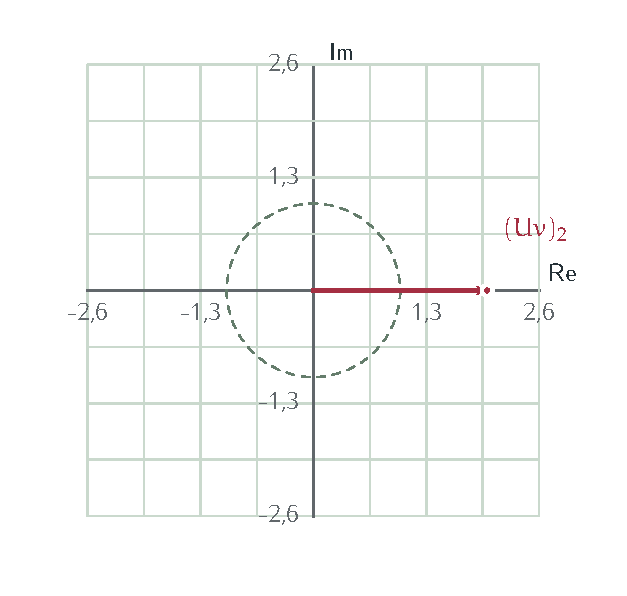
\includegraphics[width=\linewidth,height=63mm,keepaspectratio]{figure/f56fb08dee7aca4e8.pdf}\par{\sffamily\footnotesize \((Uv)_{2}\)\par}\end{minipage}\FigureCaption{2.15 \(\cdot\) esempio 2 \(\cdot\) Componenti canoniche dopo l'esponenziale}\end{FigureBlock}

\phantomsection\label{c2-funzioni-matrice-example-2-step-1}
\BookHeading{01 Richiamare la decomposizione già costruita}

\MathBlock{0050208A003D00280031002F00320029005B005B0031002C0031005D002C005B0031002C0031005D005D003B00200050208B003D00280031002F00320029005B005B0031002C22120031005D002C005B22120031002C0031005D005D}{P_{+}=(1/2)\begin{pmatrix}1&1\\1&1\end{pmatrix};\allowbreak \ P_{-}=(1/2)\begin{pmatrix}1&- 1\\- 1&1\end{pmatrix}}
\MathBlock{0041003D00340050208A002B00320050208B003B00200070003D0050208A0076003D00280033002F0032002C0033002F00320029003B00200071003D0050208B0076003D00280031002F0032002C22120031002F00320029}{A=4P_{+}+2P_{-};\allowbreak \ p=P_{+}v=(3/2{,}3/2);\allowbreak \ q=P_{-}v=(1/2,\allowbreak - 1/2)}

I proiettori sono quelli verificati nella sezione precedente; qui diventano strumenti per applicare una funzione.\par


\phantomsection\label{c2-funzioni-matrice-example-2-step-2}
\BookHeading{02 Moltiplicare due decomposizioni}

\MathBlock{004100B2003D002800340050208A002B00320050208B002900B2003D003100360050208A002B00340050208B}{A^{2}=(4P_{+}+2P_{-})^{2}=16P_{+}+4P_{-}}
\MathBlock{00410076003D00280037003B0020003500291D40003B0020004100B20076003D003100360070002B00340071003D002800320036003B00200032003200291D40}{Av=(7;\allowbreak \ 5)^{T};\allowbreak \ A^{2}v=16p+4q=(26;\allowbreak \ 22)^{T}}

I termini misti svaniscono perché \(P_{+}P_{-}=P_{-}P_{+}=0\); ogni \(P^{2}\) si riduce a \(P\).\par


\phantomsection\label{c2-funzioni-matrice-example-2-step-3}
\BookHeading{03 Definire e sommare l'esponenziale}

\MathBlock{0065005E002822120069007400410029003D03A32099208C2080221E00282212006900740029207F0041207F002F006E0021}{e^{- \text{itA}}=\sum _{n=0}\infty (- it)^{n}A^{n}/n!}
\MathBlock{003D03A32099002822120069007403BB208A0029207F0050208A002F006E0021002B03A32099002822120069007403BB208B0029207F0050208B002F006E0021}{=\sum _{n}(- it\lambda _{+})^{n}P_{+}/n!+\sum _{n}(- it\lambda _{-})^{n}P_{-}/n!}
\MathBlock{003D0065005E0028221200690034007400290050208A002B0065005E0028221200690032007400290050208B}{=e^{- i4t}P_{+}+e^{- i2t}P_{-}}

La serie scalare dell'esponenziale si applica separatamente ai due autovalori. Il parametro t è adimensionale in questo esempio algebrico.\par


\phantomsection\label{c2-funzioni-matrice-example-2-step-4}
\BookHeading{04 Sostituire un parametro preciso}

\MathBlock{0074003D03C0002F0032003A00200065005E002822120069003400740029003D0031002C00200065005E002822120069003200740029003D22120031}{t=\pi /2:\ e^{- i4t}=1,\allowbreak \ e^{- i2t}=- 1}
\MathBlock{0055003D0050208A22120050208B003D005B005B0030002C0031005D002C005B0031002C0030005D005D003B002000550076003D00280031002C00320029}{U=P_{+}- P_{-}=\begin{pmatrix}0&1\\1&0\end{pmatrix};\allowbreak \ Uv=(1{,}2)}

I fattori hanno modulo uno, quindi ruotano le componenti proprie senza cambiarne il peso.\par


\phantomsection\label{c2-funzioni-matrice-example-2-step-5}
\BookHeading{05 Verificare unitarietà e norma}

\MathBlock{005520200055003D007C0065005E002822120069007403BB208A0029007C00B20050208A002B007C0065005E002822120069007403BB208B0029007C00B20050208B003D0050208A002B0050208B003D0049}{U{}^{\dagger} U=|e^{- it\lambda _{+}}|^{2}P_{+}+|e^{- it\lambda _{-}}|^{2}P_{-}=P_{+}+P_{-}=I}
\MathBlock{201600550076201600B2003D20160076201600B2003D0035}{\Vert Uv\Vert ^{2}=\Vert v\Vert ^{2}=5}

L'esponenziale immaginario di una matrice hermitiana conserva la norma. Questa identità prepara il modello di evoluzione del modulo 3.\par


\phantomsection\label{c2-funzioni-matrice-example-2-step-6}
\BookHeading{06 Trattare uno spettro degenere}

\MathBlock{0044003D00320049003A00200075006E00690063006F0020006100750074006F00760061006C006F0072006500200032002C0020006100750074006F007300700061007A0069006F0020004300B2002C002000700072006F0069006500740074006F0072006500200050003D0049}{D=2I:\ \text{unico}\ \text{autovalore}\ 2,\allowbreak \ \text{autospazio}\ C^{2},\allowbreak \ \text{proiettore}\ P=I}
\MathBlock{0066002800440029003D00660028003200290049003B0020004400B2003D00340049003B00200065005E002822120069007400440029003D0065005E0028221200320069007400290049}{f(D)=f(2)I;\allowbreak \ D^{2}=4I;\allowbreak \ e^{- \text{itD}}=e^{- 2it}I}

Una degenerazione raccoglie l'intero autospazio. Suddividerlo in direzioni arbitrarie non cambia la funzione dell'operatore.\par


\BookHeading{Interpretazione}

Il quadrato produce \(A^{2}v=(26\); \(22)^{T}\), mentre \(e^{- \text{itA}}\) conserva la norma quadra 5. Le potenze amplificano i coefficienti propri; l'esponenziale qui svolto ne cambia le fasi.\par


\Needspace{7\baselineskip}
\BookHeading{Il passaggio successivo}
L'esponenziale immaginario conserva la norma e preparerà le evoluzioni del modulo 3. Prima di interpretare le proiezioni come esiti di misura, costruiamo il linguaggio degli eventi e delle probabilità.\par


% Authoritative exercise source. Preserve all derivations and diagrams.

\ExerciseStart{G2.10}{Ricavare autovalori, autovettori e proiettori}{Consolidamento}

\BookHeading{Problema, dati e obiettivo}

Per \(A=\begin{pmatrix}2&1\\1&2\end{pmatrix}\), trovare autovalori, autovettori normalizzati e proiettori. Ricostruire A, calcolare \(A^2\) e applicare \(e^{-itA}\) a \(e_1\) per \(t=\pi/2\). Il parametro t è adimensionale.

\ExTheory{\ExRef{c2-spettro}{2.12}; \ExRef{c2-base-propria}{2.13}; \ExRef{c2-proiettori}{2.14}; \ExRef{c2-funzioni-matrice}{2.15}}{Un autovettore soddisfa \(Au=\lambda u\), con \(u\ne0\). Gli autovalori risolvono \(\det(A-\lambda I)=0\). Per una base propria ortonormale, \(P_j=u_ju_j^\dagger\), \(A=\sum_j\lambda_jP_j\) e \(f(A)=\sum_jf(\lambda_j)P_j\).}

\ExPrediction{La matrice tratta simmetricamente le due coordinate. Le diagonali del piano sono quindi candidate naturali ad autodirezioni. La componente su ciascuna diagonale subirà un fattore indipendente.}

\ExFigure{\begin{tikzpicture}[>=Stealth,exlabel]
\draw[exaxis] (-0.35,0)--(1.55,0) node[right] {$x_1$};\draw[exaxis] (0,-1.35)--(0,1.55) node[above] {$x_2$};\draw[->,Accent,line width=1.1pt] (0,0)--(1,1) node[anchor=south west] {$ u_+\sqrt2 $};\draw[->,Secondary,line width=1.1pt] (0,0)--(1,-1) node[anchor=north west] {$ u_-\sqrt2 $};
\end{tikzpicture}}{Le due diagonali sono autodirezioni ortogonali.}


\begin{ExTasks}

\item Sviluppare il polinomio caratteristico.

\item Risolvere i due sistemi degli autovettori.

\item Normalizzare e verificare l’ortogonalità.

\item Costruire i due prodotti esterni.

\item Ricostruire A e \(A^2\).

\item Calcolare le due fasi e la loro azione su \(e_1\).

\end{ExTasks}

\ExSolution

\ExStep{Trovare gli autovalori}

\ExEq{\det(A-\lambda I)&=(2-\lambda)^2-1\\&=\lambda^2-4\lambda+3=(\lambda-3)(\lambda-1).}
Gli autovalori sono \(\lambda_+=3\) e \(\lambda_-=1\).

\ExStep{Risolvere i sistemi}

Per \(\lambda=3\), \(-u_1+u_2=0\), quindi \(u_2=u_1\). Per \(\lambda=1\), \(u_1+u_2=0\), quindi \(u_2=-u_1\). Si possono scegliere \((1,1)^T\) e \((1,-1)^T\).

\ExStep{Normalizzare e controllare}

Entrambe le norme sono \(\sqrt{1+1}=\sqrt2\):
\ExEq{u_+&=\frac1{\sqrt2}\colv{1\\1},\quad u_-=\frac1{\sqrt2}\colv{1\\-1},\\u_+^\dagger u_-&=(1-1)/2=0.}
Direttamente, \(Au_+=(3,3)^T/\sqrt2=3u_+\) e \(Au_-=(1,-1)^T/\sqrt2=u_-\).

\ExStep{Costruire i proiettori}

\ExEq{P_+&=\tfrac12\colv{1\\1}(1,1)=\tfrac12\begin{pmatrix}1&1\\1&1\end{pmatrix},\\P_-&=\tfrac12\colv{1\\-1}(1,-1)=\tfrac12\begin{pmatrix}1&-1\\-1&1\end{pmatrix}.}
La somma è I; il prodotto è zero perché \(u_+^\dagger u_-=0\).

\ExStep{Ricostruire l’operatore}

\ExEq{3P_++P_-&=\tfrac12\begin{pmatrix}3+1&3-1\\3-1&3+1\end{pmatrix}
=\begin{pmatrix}2&1\\1&2\end{pmatrix}=A.}

\ExStep{Calcolare il quadrato}

\ExEq{A^2&=9P_++P_-=\tfrac12\begin{pmatrix}10&8\\8&10\end{pmatrix}
=\begin{pmatrix}5&4\\4&5\end{pmatrix}.}
La moltiplicazione diretta produce elementi \(2\cdot2+1\cdot1=5\) e \(2\cdot1+1\cdot2=4\), con gli altri due ottenuti analogamente dalle rispettive righe.

\ExStep{Assegnare le fasi alle autodirezioni}

\ExEq{e^{-itA}&=e^{-3it}P_++e^{-it}P_-,\\e^{-3i\pi/2}&=i,\qquad e^{-i\pi/2}=-i,\\e^{-i\pi A/2}&=i(P_+-P_-)=i\begin{pmatrix}0&1\\1&0\end{pmatrix}.}

\ExStep{Applicare e interpretare}

\ExEq{e^{-i\pi A/2}e_1&=i\colv{0\\1}.}
La norma finale è uno. Se A rappresentasse un Hamiltoniano diviso per una scala energetica e t fosse il tempo corrispondentemente riscalato, l’esponenziale descriverebbe l’evoluzione. Le due componenti proprie accumulano fasi differenti prima di ricombinarsi.

\par\noindent\begin{minipage}{\linewidth}
\ExFigure{\begin{tikzpicture}[>=Stealth,exlabel]
\node[exbox] (n0) at (0.0,0.0) {$e_1=(u_++u_-)/\sqrt2$};\node[exbox] (n1) at (3.6,0.0) {fattori $i,-i$};\draw[exother] (n0)--(n1);\node[exbox] (n2) at (7.2,0.0) {$i e_2$};\draw[exother] (n1)--(n2);
\end{tikzpicture}}{Scomposizione, evoluzione delle fasi e ricomposizione del vettore.}


\ExInterpret{La base propria separa l’azione dell’operatore in trasformazioni scalari. I proiettori riportano ciascuna componente nello spazio originario, permettendo di verificare il risultato senza cambiare il significato geometrico del vettore.}

\ExLab{Nelle sezioni 2.12–2.15 confrontare autovalori, base propria e proiettori della matrice assegnata. Nello strumento matriciale verificare \(A^2\) per moltiplicazione diretta. Le figure delle autodirezioni devono conservare la stessa convenzione di base.}


\end{minipage}

\Needspace{.43\textheight}
\section{Dagli esiti agli eventi}
\phantomsection\label{c2-eventi}

{\sffamily\small\color{Ink!70} Riferimento alle slide: p. 217.\par}

{\sffamily\small\color{Ink!70} Laboratorio locale: \nolinkurl{index.html#capitolo-2/eventi}\par}

\BookHeading{Definizioni e costruzione}
Un evento è un insieme di esiti. La sua probabilità si ottiene sommando i pesi degli esiti che lo compongono.\par

Lo spazio degli esiti elenca le alternative elementari dell'esperimento. \(A\) ciascuna alternativa è assegnata una probabilità non negativa, e la somma su tutte le alternative vale uno. Un evento può comprendere una sola alternativa, più alternative oppure nessuna.\par

Le probabilità degli esiti distinti si sommano perché gli esiti sono mutuamente esclusivi. Nel calcolo dell'unione di due eventi, l'intersezione verrebbe contata due volte; sottrarla restituisce il peso corretto. L'evento impossibile ha probabilità zero e quello certo probabilità uno.\par


\MathBlock{0050002800410029003D03A303C9220800410020007003C9003B0020005000280041222A00420029003D0050002800410029002B00500028004200292212005000280041222900420029002E}{P(A)=\sum _{\omega \in A}\ p\omega ;\allowbreak \ P(A\cup B)=P(A)+P(B)- P(A\cap B).}

\BookHeading{Come leggere le figure}
Barre di probabilità: lunghezza proporzionale al peso, etichette discrete.\par


\Needspace{.36\textheight}\phantomsection\label{c2-eventi-example-1}
{\sffamily\small\color{Accent} ESEMPIO SVOLTO 1\par}
\BookHeading{Eventi sovrapposti}
Dati gli esiti \(\Omega =\{0{,}1{,}2{,}3\}\) con probabilità (1/10, 2/10, 3/10, 4/10).\par


\BookHeading{Geometria e configurazione dell'esempio}
\begin{FigureBlock}\centering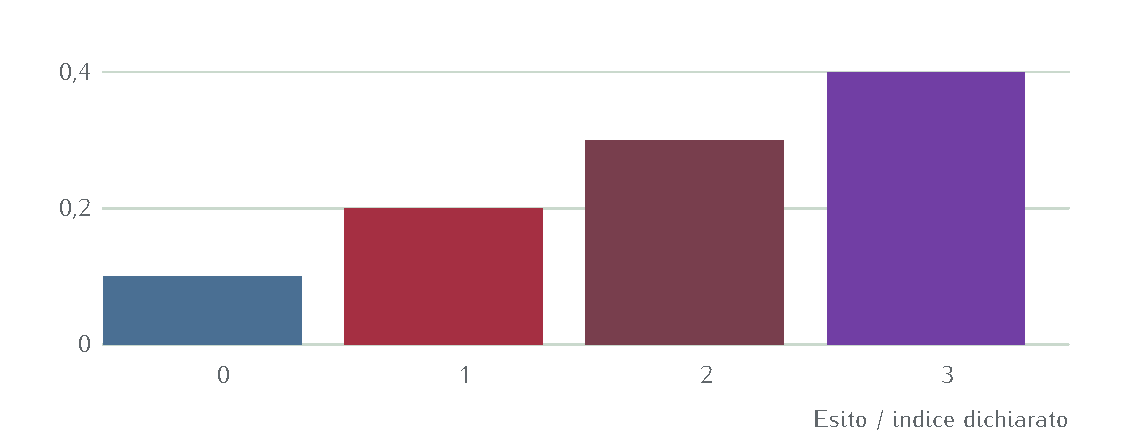
\includegraphics[width=\linewidth,height=94mm,keepaspectratio]{figure/ffccb9f38494ac157.pdf}\FigureCaption{2.16 \(\cdot\) esempio 1 \(\cdot\) Probabilità degli esiti elementari}\end{FigureBlock}

\phantomsection\label{c2-eventi-example-1-step-1}
\BookHeading{01 Verificare la distribuzione assegnata}

\MathBlock{03A9003D007B0030002C0031002C0032002C0033007D003B00200070003D00280031002F00310030002C0032002F00310030002C0033002F00310030002C0034002F003100300029}{\Omega =\{0{,}1{,}2{,}3\};\allowbreak \ p=(1/10{,}2/10{,}3/10{,}4/10)}
\MathBlock{03A30070003D00280031002B0032002B0033002B00340029002F00310030003D0031}{\sum p=(1+2+3+4)/10=1}

Le quattro probabilità sono dati dell'esperimento e sono tutte non negative.\par


\phantomsection\label{c2-eventi-example-1-step-2}
\BookHeading{02 Sommarne i pesi sugli eventi}

\MathBlock{0041003D007B0030002C0032007D003B00200042003D007B0032002C0033007D}{A=\{0{,}2\};\allowbreak \ B=\{2{,}3\}}
\MathBlock{0050002800410029003D0031002F00310030002B0033002F00310030003D0030002C0034}{P(A)=1/10+3/10=0{,}4}
\MathBlock{0050002800420029003D0033002F00310030002B0034002F00310030003D0030002C0037}{P(B)=3/10+4/10=0{,}7}

Un evento è un insieme di etichette; ciascun esito viene contato una sola volta.\par


\phantomsection\label{c2-eventi-example-1-step-3}
\BookHeading{03 Calcolare intersezione e unione}

\MathBlock{004122290042003D007B0032007D003B0020005000280041222900420029003D0030002C0033}{A\cap B=\{2\};\allowbreak \ P(A\cap B)=0{,}3}
\MathBlock{0041222A0042003D007B0030002C0032002C0033007D003B0020005000280041222A00420029003D0030002C0034002B0030002C003722120030002C0033003D0030002C0038}{A\cup B=\{0{,}2{,}3\};\allowbreak \ P(A\cup B)=0{,}4+0{,}7- 0{,}3=0{,}8}

Il termine dell'intersezione corregge il doppio conteggio degli esiti comuni.\par


\phantomsection\label{c2-eventi-example-1-step-4}
\BookHeading{04 Includere eventi certo e impossibile}

\MathBlock{0050002803A90029003D0031003B00200050002822050029003D0030003B00200050002803A9005C00410029003D003122120050002800410029}{P(\Omega )=1;\allowbreak \ P(\varnothing )=0;\allowbreak \ P(\Omega \backslash A)=1- P(A)}

La somma sull'insieme vuoto non contiene contributi; il complemento raccoglie tutti gli esiti rimanenti.\par


\BookHeading{Interpretazione}

L'esito 2 appartiene a entrambi gli eventi; sottrarne una volta il peso evita di contarlo due volte.\par


\Needspace{.36\textheight}\phantomsection\label{c2-eventi-example-2}
{\sffamily\small\color{Accent} ESEMPIO SVOLTO 2\par}
\BookHeading{Eventi disgiunti ed esaustivi}
Dati gli esiti \(\Omega =\{0{,}1{,}2{,}3\}\) con probabilità (1/8, 1/8, 2/8, 4/8).\par


\BookHeading{Geometria e configurazione dell'esempio}
\begin{FigureBlock}\centering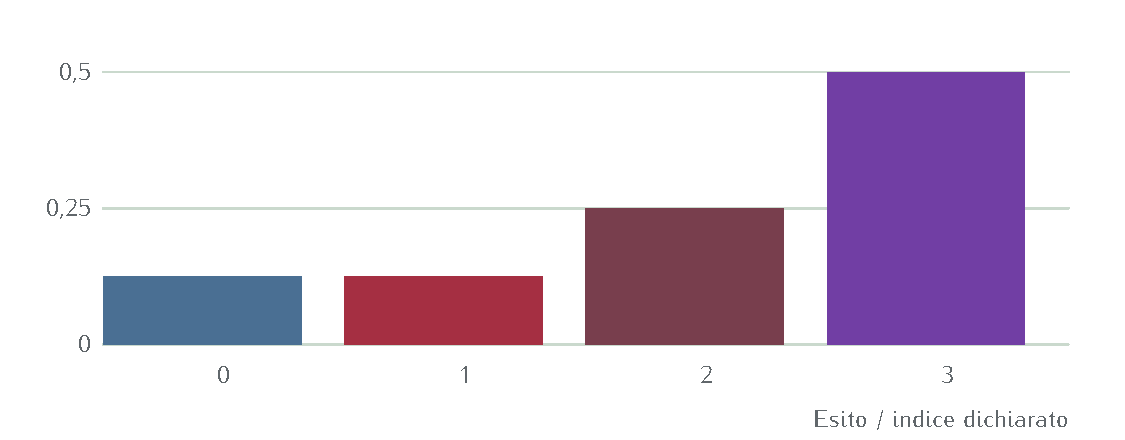
\includegraphics[width=\linewidth,height=94mm,keepaspectratio]{figure/f1419ea2ef5bba520.pdf}\FigureCaption{2.16 \(\cdot\) esempio 2 \(\cdot\) Probabilità degli esiti elementari}\end{FigureBlock}

\phantomsection\label{c2-eventi-example-2-step-1}
\BookHeading{01 Verificare la distribuzione assegnata}

\MathBlock{03A9003D007B0030002C0031002C0032002C0033007D003B00200070003D00280031002F0038002C0031002F0038002C0032002F0038002C0034002F00380029}{\Omega =\{0{,}1{,}2{,}3\};\allowbreak \ p=(1/8{,}1/8{,}2/8{,}4/8)}
\MathBlock{03A30070003D00280031002B0031002B0032002B00340029002F0038003D0031}{\sum p=(1+1+2+4)/8=1}

Le quattro probabilità sono dati dell'esperimento e sono tutte non negative.\par


\phantomsection\label{c2-eventi-example-2-step-2}
\BookHeading{02 Sommarne i pesi sugli eventi}

\MathBlock{0041003D007B0030002C0031007D003B00200042003D007B0032002C0033007D}{A=\{0{,}1\};\allowbreak \ B=\{2{,}3\}}
\MathBlock{0050002800410029003D0031002F0038002B0031002F0038003D0030002C00320035}{P(A)=1/8+1/8=0{,}25}
\MathBlock{0050002800420029003D0032002F0038002B0034002F0038003D0030002C00370035}{P(B)=2/8+4/8=0{,}75}

Un evento è un insieme di etichette; ciascun esito viene contato una sola volta.\par


\phantomsection\label{c2-eventi-example-2-step-3}
\BookHeading{03 Calcolare intersezione e unione}

\MathBlock{004122290042003D2205003B0020005000280041222900420029003D0030}{A\cap B=\varnothing ;\allowbreak \ P(A\cap B)=0}
\MathBlock{0041222A0042003D007B0030002C0031002C0032002C0033007D003B0020005000280041222A00420029003D0030002C00320035002B0030002C0037003522120030003D0031}{A\cup B=\{0{,}1{,}2{,}3\};\allowbreak \ P(A\cup B)=0{,}25+0{,}75- 0=1}

Il termine dell'intersezione corregge il doppio conteggio degli esiti comuni.\par


\phantomsection\label{c2-eventi-example-2-step-4}
\BookHeading{04 Includere eventi certo e impossibile}

\MathBlock{0050002803A90029003D0031003B00200050002822050029003D0030003B00200050002803A9005C00410029003D003122120050002800410029}{P(\Omega )=1;\allowbreak \ P(\varnothing )=0;\allowbreak \ P(\Omega \backslash A)=1- P(A)}

La somma sull'insieme vuoto non contiene contributi; il complemento raccoglie tutti gli esiti rimanenti.\par


\BookHeading{Interpretazione}

\(A\) e \(B\) sono disgiunti e la loro unione è \(\Omega \), quindi \(P(A)+P(B)=1\).\par


\Needspace{7\baselineskip}
\BookHeading{Il passaggio successivo}
Un evento raccoglie etichette. Una variabile raggrupperà gli stessi esiti secondo i valori assegnati, producendo una nuova distribuzione.\par


\Needspace{.43\textheight}
\section{Normalizzare e raggruppare i pesi}
\phantomsection\label{c2-distribuzioni}

{\sffamily\small\color{Ink!70} Riferimento alle slide: p. 223.\par}

{\sffamily\small\color{Ink!70} Laboratorio locale: \nolinkurl{index.html#capitolo-2/distribuzioni}\par}

\BookHeading{Definizioni e costruzione}
I pesi positivi diventano probabilità dopo averne calcolato il totale. Una variabile associa un numero a ciascun esito e può riunire più esiti nello stesso valore.\par

Un insieme di pesi positivi può descrivere frequenze grezze, conteggi o intensità relative. Dividendo ciascun peso per il totale si ottiene una distribuzione di probabilità. Moltiplicare tutti i pesi per lo stesso fattore positivo conserva la distribuzione.\par

Una variabile aleatoria assegna un valore a ciascun esito. Se più esiti ricevono lo stesso valore, le loro probabilità vengono riunite. Occorre quindi distinguere l'etichetta dell'esito dal valore della variabile: questa distinzione permette di interpretare correttamente grafici e medie.\par


\MathBlock{00702C7C003D00772C7C002F03A3209600772096003B0020005000280058003D00780029003D03A32C7C003A00582C7C003D0078002000702C7C002E}{p_{j}=w_{j}/\sum _{k}w_{k};\allowbreak \ P(X=x)=\sum _{j}:X_{j}=x\ p_{j}.}

\BookHeading{Come leggere le figure}
Distribuzione discreta, con somma delle probabilità uguale a uno.\par


\Needspace{.36\textheight}\phantomsection\label{c2-distribuzioni-example-1}
{\sffamily\small\color{Accent} ESEMPIO SVOLTO 1\par}
\BookHeading{Dai pesi alla variabile di parità}
Dati pesi (1, 2, 3, 4) sulle etichette 0,1,2,3.\par


\BookHeading{Geometria e configurazione dell'esempio}
\begin{FigureBlock}\centering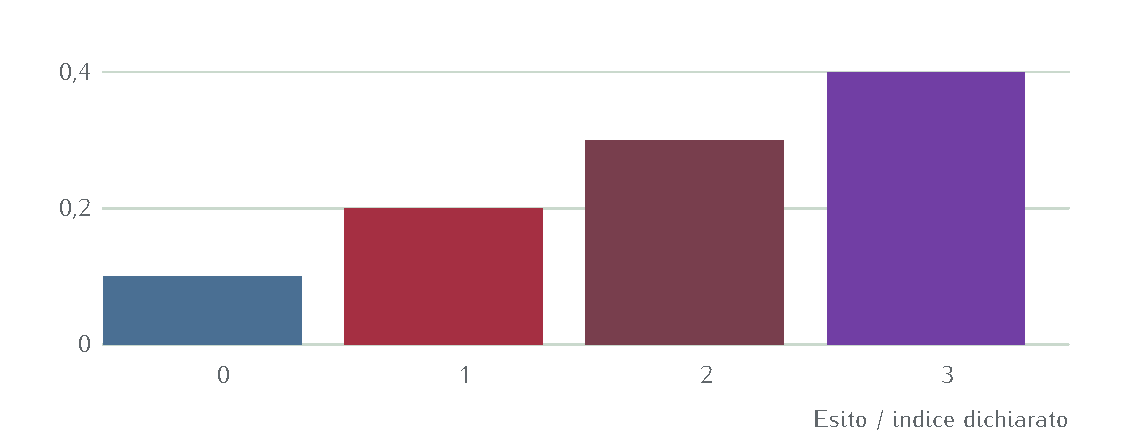
\includegraphics[width=\linewidth,height=94mm,keepaspectratio]{figure/f77d7cf4e26333859.pdf}\FigureCaption{2.17 \(\cdot\) esempio 1 \(\cdot\) Distribuzione sulle quattro etichette}\end{FigureBlock}
\begin{FigureBlock}\centering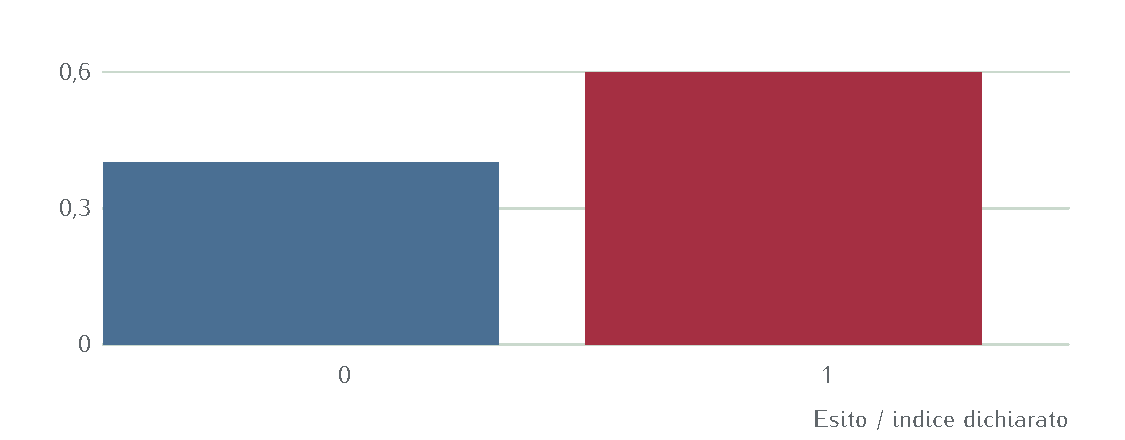
\includegraphics[width=\linewidth,height=94mm,keepaspectratio]{figure/f1ccd81ddd4b2a5e7.pdf}\FigureCaption{2.17 \(\cdot\) esempio 1 \(\cdot\) Distribuzione della variabile \(X\)}\end{FigureBlock}

\phantomsection\label{c2-distribuzioni-example-1-step-1}
\BookHeading{01 Normalizzare i pesi}

\MathBlock{0057003D0031002B0032002B0033002B0034003D00310030}{W=1+2+3+4=10}
\MathBlock{0070003D00280031002F00310030002C00200032002F00310030002C00200033002F00310030002C00200034002F003100300029}{p=(1/10,\allowbreak \ 2/10,\allowbreak \ 3/10,\allowbreak \ 4/10)}
\MathBlock{03A30070003D0031}{\sum p=1}

Il totale positivo permette di dividere tutti i pesi per lo stesso numero.\par


\phantomsection\label{c2-distribuzioni-example-1-step-2}
\BookHeading{02 Assegnare una variabile}

\MathBlock{0058002800300029003D0030003B00200058002800310029003D0031003B00200058002800320029003D0030003B00200058002800330029003D0031}{X(0)=0;\allowbreak \ X(1)=1;\allowbreak \ X(2)=0;\allowbreak \ X(3)=1}

La variabile assegna un valore numerico a ciascuna etichetta dell'esito.\par


\phantomsection\label{c2-distribuzioni-example-1-step-3}
\BookHeading{03 Raggruppare il valore 0}

\MathBlock{005000280058003D00300029003D0031002F00310030002B0033002F00310030003D0030002C0034}{P(X=0)=1/10+3/10=0{,}4}

Si sommano i pesi di tutte le etichette che ricevono lo stesso valore.\par


\phantomsection\label{c2-distribuzioni-example-1-step-4}
\BookHeading{04 Raggruppare il valore 1}

\MathBlock{005000280058003D00310029003D0032002F00310030002B0034002F00310030003D0030002C0036}{P(X=1)=2/10+4/10=0{,}6}

Si sommano i pesi di tutte le etichette che ricevono lo stesso valore.\par


\phantomsection\label{c2-distribuzioni-example-1-step-5}
\BookHeading{05 Controllare l'invarianza di scala}

\MathBlock{00772032003D00320077003D00280032002C0034002C0036002C00380029003B002000572032003D00320030}{w{}^{\prime} =2w=(2{,}4{,}6{,}8);\allowbreak \ W{}^{\prime} =20}
\MathBlock{007720322C7C002F00572032003D003200772C7C002F0028003200570029003D00772C7C002F0057}{w{}^{\prime} _{j}/W{}^{\prime} =2w_{j}/(2W)=w_{j}/W}

Raddoppiare tutti i pesi conserva la distribuzione. Se tutti fossero nulli, \(W=0\) impedirebbe la normalizzazione.\par


\BookHeading{Interpretazione}

La variabile ha due valori con probabilità (0,4, 0,6). Il raggruppamento riduce le etichette conservando il peso totale.\par


\Needspace{.36\textheight}\phantomsection\label{c2-distribuzioni-example-2}
{\sffamily\small\color{Accent} ESEMPIO SVOLTO 2\par}
\BookHeading{Raggruppamento per una seconda variabile}
Dati pesi (1, 1, 2, 4) sulle etichette 0,1,2,3.\par


\BookHeading{Geometria e configurazione dell'esempio}
\begin{FigureBlock}\centering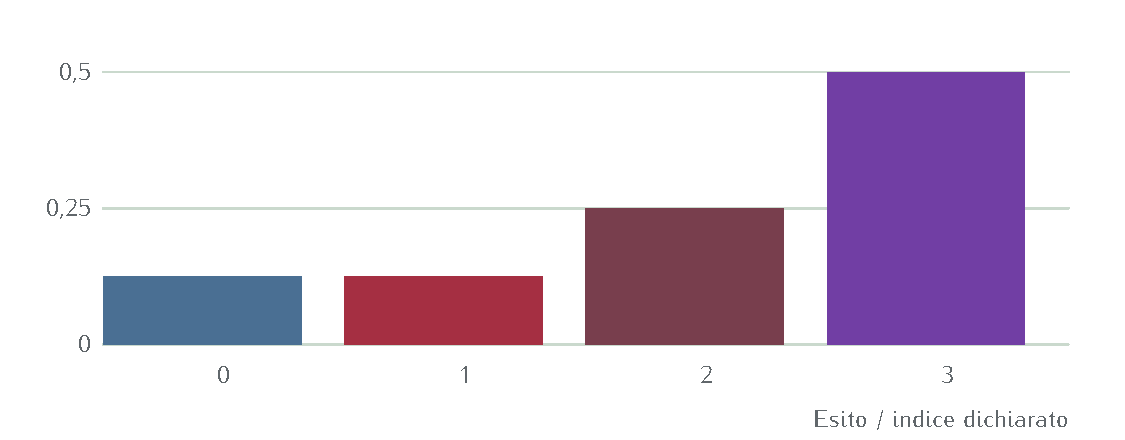
\includegraphics[width=\linewidth,height=94mm,keepaspectratio]{figure/f12272e8fb2233632.pdf}\FigureCaption{2.17 \(\cdot\) esempio 2 \(\cdot\) Distribuzione sulle quattro etichette}\end{FigureBlock}
\begin{FigureBlock}\centering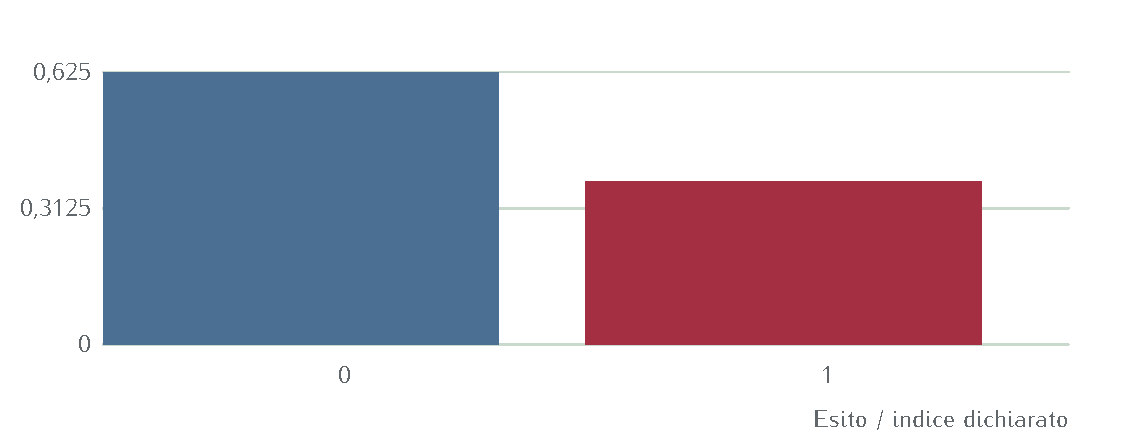
\includegraphics[width=\linewidth,height=94mm,keepaspectratio]{figure/f40d13226ff20dde8.pdf}\FigureCaption{2.17 \(\cdot\) esempio 2 \(\cdot\) Distribuzione della variabile \(X\)}\end{FigureBlock}

\phantomsection\label{c2-distribuzioni-example-2-step-1}
\BookHeading{01 Normalizzare i pesi}

\MathBlock{0057003D0031002B0031002B0032002B0034003D0038}{W=1+1+2+4=8}
\MathBlock{0070003D00280031002F0038002C00200031002F0038002C00200032002F0038002C00200034002F00380029}{p=(1/8,\allowbreak \ 1/8,\allowbreak \ 2/8,\allowbreak \ 4/8)}
\MathBlock{03A30070003D0031}{\sum p=1}

Il totale positivo permette di dividere tutti i pesi per lo stesso numero.\par


\phantomsection\label{c2-distribuzioni-example-2-step-2}
\BookHeading{02 Assegnare una variabile}

\MathBlock{0058002800300029003D0030003B00200058002800310029003D0031003B00200058002800320029003D0031003B00200058002800330029003D0030}{X(0)=0;\allowbreak \ X(1)=1;\allowbreak \ X(2)=1;\allowbreak \ X(3)=0}

La variabile assegna un valore numerico a ciascuna etichetta dell'esito.\par


\phantomsection\label{c2-distribuzioni-example-2-step-3}
\BookHeading{03 Raggruppare il valore 0}

\MathBlock{005000280058003D00300029003D0031002F0038002B0034002F0038003D0030002C003600320035}{P(X=0)=1/8+4/8=0{,}625}

Si sommano i pesi di tutte le etichette che ricevono lo stesso valore.\par


\phantomsection\label{c2-distribuzioni-example-2-step-4}
\BookHeading{04 Raggruppare il valore 1}

\MathBlock{005000280058003D00310029003D0031002F0038002B0032002F0038003D0030002C003300370035}{P(X=1)=1/8+2/8=0{,}375}

Si sommano i pesi di tutte le etichette che ricevono lo stesso valore.\par


\phantomsection\label{c2-distribuzioni-example-2-step-5}
\BookHeading{05 Controllare l'invarianza di scala}

\MathBlock{00772032003D00320077003D00280032002C0032002C0034002C00380029003B002000572032003D00310036}{w{}^{\prime} =2w=(2{,}2{,}4{,}8);\allowbreak \ W{}^{\prime} =16}
\MathBlock{007720322C7C002F00572032003D003200772C7C002F0028003200570029003D00772C7C002F0057}{w{}^{\prime} _{j}/W{}^{\prime} =2w_{j}/(2W)=w_{j}/W}

Raddoppiare tutti i pesi conserva la distribuzione. Se tutti fossero nulli, \(W=0\) impedirebbe la normalizzazione.\par


\BookHeading{Interpretazione}

La variabile ha due valori con probabilità (0,625, 0,375). Il raggruppamento riduce le etichette conservando il peso totale.\par


\Needspace{7\baselineskip}
\BookHeading{Il passaggio successivo}
Dopo aver normalizzato e raggruppato i pesi, li useremo per calcolare il baricentro dei valori e la dispersione intorno a esso.\par


\Needspace{.43\textheight}
\section{Media e dispersione}
\phantomsection\label{c2-momenti}

{\sffamily\small\color{Ink!70} Riferimento alle slide: p. 229.\par}

{\sffamily\small\color{Ink!70} Laboratorio locale: \nolinkurl{index.html#capitolo-2/momenti}\par}

\BookHeading{Definizioni e costruzione}
La media è il baricentro della distribuzione. La varianza pesa i quadrati degli scarti, così che gli scarti di segno opposto contribuiscano entrambi.\par

Il valore atteso pesa ogni valore con la sua probabilità. È il risultato verso cui tende la media di molte prove nelle condizioni della legge dei grandi numeri; può differire da ciascuno degli esiti possibili di una singola prova.\par

La varianza pesa gli scarti quadratici rispetto alla media. Sviluppando \((x- \mu )^{2}\) e usando \(\sum p=1\) ed \(E[X]=\mu \) si ricava \(E[X^{2}]- \mu ^{2}\). La varianza ha unità di misura al quadrato; la deviazione standard, ottenuta estraendo la radice, ha le stesse unità della variabile.\par


\MathBlock{0045005B0058005D003D03A3007800200070002800780029003B0020005600610072002800580029003D03A300700028007800290028007822120045005B0058005D002900B2003D0045005B005800B2005D22120045005B0058005D00B2002E}{E[X]=\sum _{x}\ p(x);\allowbreak \ \operatorname{Var}(X)=\sum p(x)(x- E[X])^{2}=E[X^{2}]- E[X]^{2}.}

\BookHeading{Come leggere le figure}
Asse dei valori e pesi discreti; la media può cadere fra gli esiti.\par


\Needspace{.36\textheight}\phantomsection\label{c2-momenti-example-1}
{\sffamily\small\color{Accent} ESEMPIO SVOLTO 1\par}
\BookHeading{Media intera con dispersione positiva}
Dati \(X\in \{0{,}1{,}2{,}3\}\) con pesi (1, 2, 3, 4), valori adimensionali.\par


\BookHeading{Geometria e configurazione dell'esempio}
\begin{FigureBlock}\centering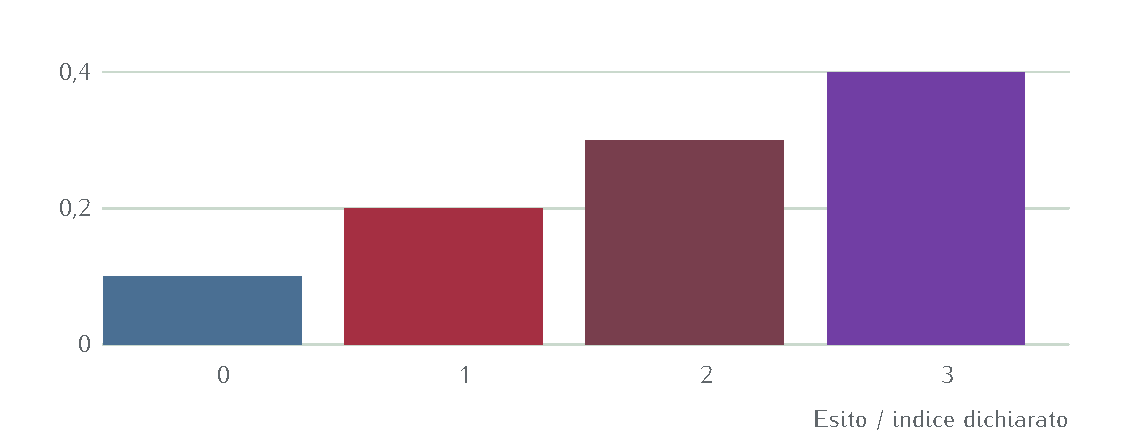
\includegraphics[width=\linewidth,height=94mm,keepaspectratio]{figure/fd748b8a651f2f45a.pdf}\FigureCaption{2.18 \(\cdot\) esempio 1 \(\cdot\) Probabilità dei valori di \(X\)}\end{FigureBlock}
\begin{FigureBlock}\centering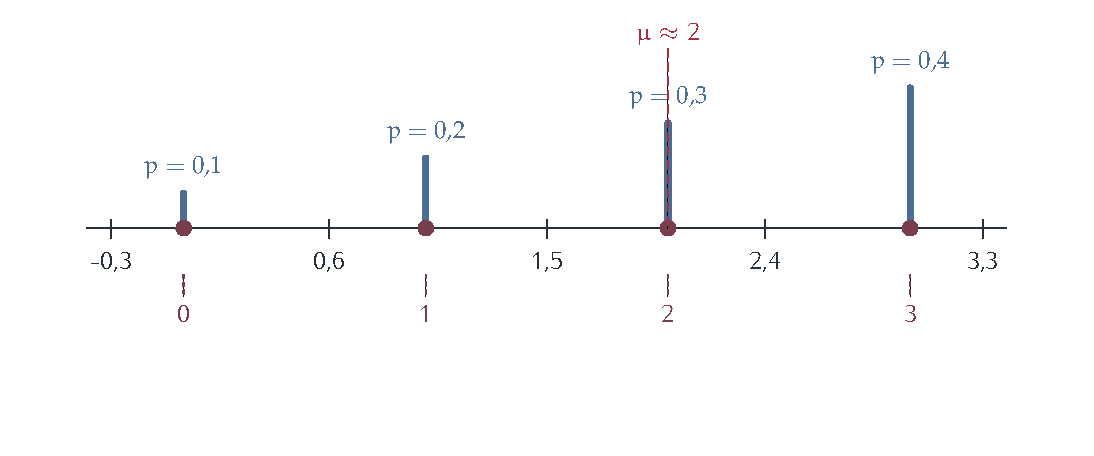
\includegraphics[width=\linewidth,height=94mm,keepaspectratio]{figure/f07b980cf3dc8ab2f.pdf}\FigureCaption{2.18 \(\cdot\) esempio 1 \(\cdot\) Baricentro \(\mu \) e distanze dei valori dalla media}\end{FigureBlock}

\phantomsection\label{c2-momenti-example-1-step-1}
\BookHeading{01 Normalizzare i pesi}

\MathBlock{0057003D0031002B0032002B0033002B0034003D00310030}{W=1+2+3+4=10}
\MathBlock{0070003D00280031002F00310030002C00200032002F00310030002C00200033002F00310030002C00200034002F003100300029}{p=(1/10,\allowbreak \ 2/10,\allowbreak \ 3/10,\allowbreak \ 4/10)}
\MathBlock{03A30070003D0031}{\sum p=1}

Il totale positivo permette di dividere tutti i pesi per lo stesso numero.\par


\phantomsection\label{c2-momenti-example-1-step-2}
\BookHeading{02 Definire i valori e calcolare la media}

\MathBlock{00580028006A0029003D006A002C0020006A003D0030002C0031002C0032002C0033}{X(j)=j,\allowbreak \ j=0{,}1{,}2{,}3}
\MathBlock{03BC003D0045005B0058005D003D003000B70031002F00310030002B003100B70032002F00310030002B003200B70033002F00310030002B003300B70034002F00310030003D0032}{\mu =E[X]=0\cdot 1/10+1\cdot 2/10+2\cdot 3/10+3\cdot 4/10=2}

I valori sono numeri adimensionali; la media è il baricentro dei pesi lungo questo asse.\par


\phantomsection\label{c2-momenti-example-1-step-3}
\BookHeading{03 Calcolare il secondo momento}

\MathBlock{0045005B005800B2005D003D003000B200B70031002F00310030002B003100B200B70032002F00310030002B003200B200B70033002F00310030002B003300B200B70034002F00310030003D0035}{E[X^{2}]=0^{2}\cdot 1/10+1^{2}\cdot 2/10+2^{2}\cdot 3/10+3^{2}\cdot 4/10=5}

Si eleva al quadrato ciascun valore prima di moltiplicarlo per il suo peso.\par


\phantomsection\label{c2-momenti-example-1-step-4}
\BookHeading{04 Esporre tutti gli scarti}

\MathBlock{0078003D0030003A00200078221203BC003D002D0032003B0020007000280078002900280078221203BC002900B2003D0031002F0031003000B70028002D0032002900B2003D0030002C0034}{x=0:\ x- \mu =-2;\allowbreak \ p(x)(x- \mu )^{2}=1/10\cdot (-2)^{2}=0{,}4}
\MathBlock{0078003D0031003A00200078221203BC003D002D0031003B0020007000280078002900280078221203BC002900B2003D0032002F0031003000B70028002D0031002900B2003D0030002C0032}{x=1:\ x- \mu =-1;\allowbreak \ p(x)(x- \mu )^{2}=2/10\cdot (-1)^{2}=0{,}2}
\MathBlock{0078003D0032003A00200078221203BC003D0030003B0020007000280078002900280078221203BC002900B2003D0033002F0031003000B700280030002900B2003D0030}{x=2:\ x- \mu =0;\allowbreak \ p(x)(x- \mu )^{2}=3/10\cdot (0)^{2}=0}
\MathBlock{0078003D0033003A00200078221203BC003D0031003B0020007000280078002900280078221203BC002900B2003D0034002F0031003000B700280031002900B2003D0030002C0034}{x=3:\ x- \mu =1;\allowbreak \ p(x)(x- \mu )^{2}=4/10\cdot (1)^{2}=0{,}4}

Gli scarti possono avere segno diverso; il quadrato ne misura il contributo non negativo alla dispersione.\par


\phantomsection\label{c2-momenti-example-1-step-5}
\BookHeading{05 Verificare la varianza in due modi}

\MathBlock{03A3007000280078002900280078221203BC002900B2003D0031}{\sum p(x)(x- \mu )^{2}=1}
\MathBlock{0045005B005800B2005D221203BC00B2003D0035221200280032002900B2003D0031003B002003C3003D221A003122480031}{E[X^{2}]- \mu ^{2}=5- (2)^{2}=1;\allowbreak \ \sigma =\sqrt{1}\approx 1}

Le due formule coincidono; una variabile costante avrebbe tutti gli scarti nulli.\par


\BookHeading{Interpretazione}

La media è 2 e la varianza 1. Le distanze dalla media vengono pesate dalla probabilità, come mostrano l'asse dei valori e i contributi quadratici.\par


\Needspace{.36\textheight}\phantomsection\label{c2-momenti-example-2}
{\sffamily\small\color{Accent} ESEMPIO SVOLTO 2\par}
\BookHeading{Pesi concentrati verso il valore massimo}
Dati \(X\in \{0{,}1{,}2{,}3\}\) con pesi (1, 1, 2, 4), valori adimensionali.\par


\BookHeading{Geometria e configurazione dell'esempio}
\begin{FigureBlock}\centering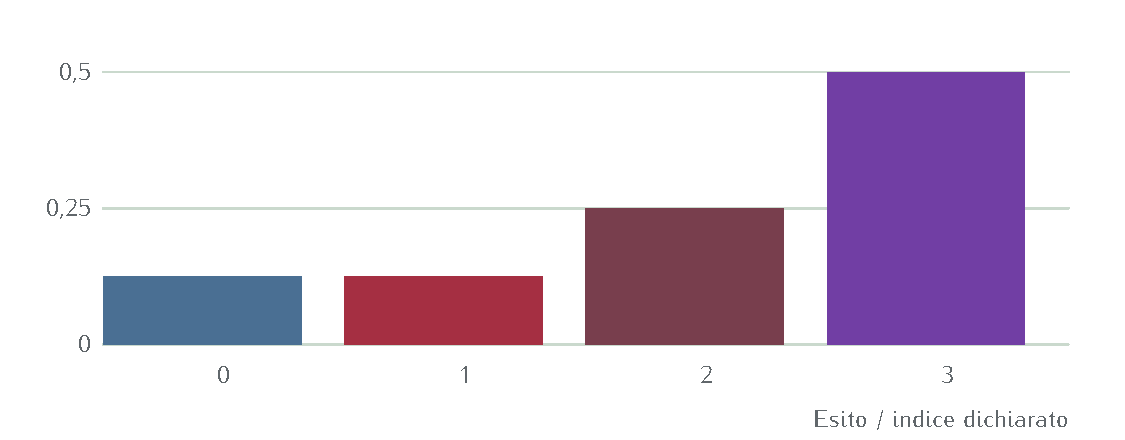
\includegraphics[width=\linewidth,height=94mm,keepaspectratio]{figure/fa1126e06dd07e193.pdf}\FigureCaption{2.18 \(\cdot\) esempio 2 \(\cdot\) Probabilità dei valori di \(X\)}\end{FigureBlock}
\begin{FigureBlock}\centering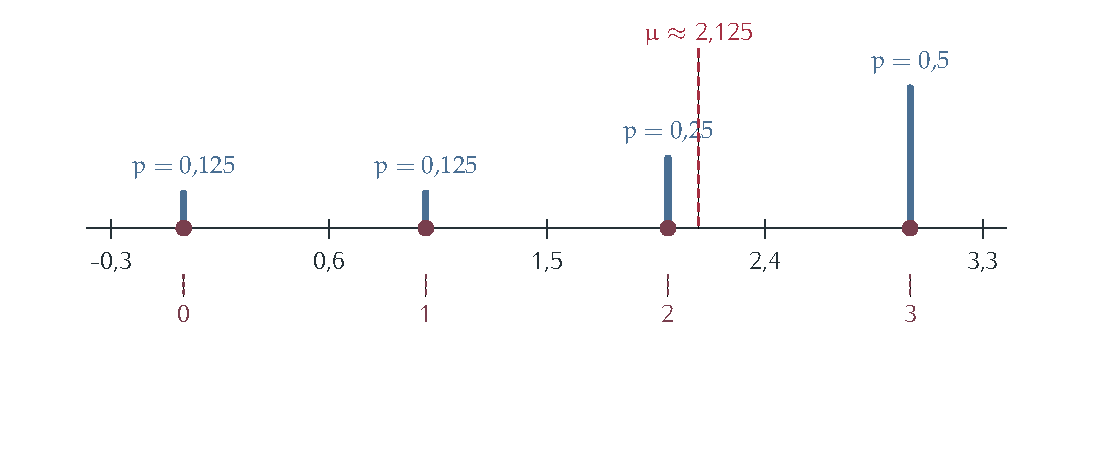
\includegraphics[width=\linewidth,height=94mm,keepaspectratio]{figure/ffefa5b93776815b3.pdf}\FigureCaption{2.18 \(\cdot\) esempio 2 \(\cdot\) Baricentro \(\mu \) e distanze dei valori dalla media}\end{FigureBlock}

\phantomsection\label{c2-momenti-example-2-step-1}
\BookHeading{01 Normalizzare i pesi}

\MathBlock{0057003D0031002B0031002B0032002B0034003D0038}{W=1+1+2+4=8}
\MathBlock{0070003D00280031002F0038002C00200031002F0038002C00200032002F0038002C00200034002F00380029}{p=(1/8,\allowbreak \ 1/8,\allowbreak \ 2/8,\allowbreak \ 4/8)}
\MathBlock{03A30070003D0031}{\sum p=1}

Il totale positivo permette di dividere tutti i pesi per lo stesso numero.\par


\phantomsection\label{c2-momenti-example-2-step-2}
\BookHeading{02 Definire i valori e calcolare la media}

\MathBlock{00580028006A0029003D006A002C0020006A003D0030002C0031002C0032002C0033}{X(j)=j,\allowbreak \ j=0{,}1{,}2{,}3}
\MathBlock{03BC003D0045005B0058005D003D003000B70031002F0038002B003100B70031002F0038002B003200B70032002F0038002B003300B70034002F0038003D0032002C003100320035}{\mu =E[X]=0\cdot 1/8+1\cdot 1/8+2\cdot 2/8+3\cdot 4/8=2{,}125}

I valori sono numeri adimensionali; la media è il baricentro dei pesi lungo questo asse.\par


\phantomsection\label{c2-momenti-example-2-step-3}
\BookHeading{03 Calcolare il secondo momento}

\MathBlock{0045005B005800B2005D003D003000B200B70031002F0038002B003100B200B70031002F0038002B003200B200B70032002F0038002B003300B200B70034002F0038003D0035002C003600320035}{E[X^{2}]=0^{2}\cdot 1/8+1^{2}\cdot 1/8+2^{2}\cdot 2/8+3^{2}\cdot 4/8=5{,}625}

Si eleva al quadrato ciascun valore prima di moltiplicarlo per il suo peso.\par


\phantomsection\label{c2-momenti-example-2-step-4}
\BookHeading{04 Esporre tutti gli scarti}

\MathBlock{0078003D0030003A00200078221203BC003D002D0032002C003100320035003B0020007000280078002900280078221203BC002900B2003D0031002F003800B70028002D0032002C003100320035002900B2003D0030002C0035003600340035}{x=0:\ x- \mu =-2{,}125;\allowbreak \ p(x)(x- \mu )^{2}=1/8\cdot (-2{,}125)^{2}=0{,}5645}
\MathBlock{0078003D0031003A00200078221203BC003D002D0031002C003100320035003B0020007000280078002900280078221203BC002900B2003D0031002F003800B70028002D0031002C003100320035002900B2003D0030002C0031003500380032}{x=1:\ x- \mu =-1{,}125;\allowbreak \ p(x)(x- \mu )^{2}=1/8\cdot (-1{,}125)^{2}=0{,}1582}
\MathBlock{0078003D0032003A00200078221203BC003D002D0030002C003100320035003B0020007000280078002900280078221203BC002900B2003D0032002F003800B70028002D0030002C003100320035002900B2003D0030002C0030003000330039}{x=2:\ x- \mu =-0{,}125;\allowbreak \ p(x)(x- \mu )^{2}=2/8\cdot (-0{,}125)^{2}=0{,}0039}
\MathBlock{0078003D0033003A00200078221203BC003D0030002C003800370035003B0020007000280078002900280078221203BC002900B2003D0034002F003800B700280030002C003800370035002900B2003D0030002C0033003800320038}{x=3:\ x- \mu =0{,}875;\allowbreak \ p(x)(x- \mu )^{2}=4/8\cdot (0{,}875)^{2}=0{,}3828}

Gli scarti possono avere segno diverso; il quadrato ne misura il contributo non negativo alla dispersione.\par


\phantomsection\label{c2-momenti-example-2-step-5}
\BookHeading{05 Verificare la varianza in due modi}

\MathBlock{03A3007000280078002900280078221203BC002900B2003D0031002C0031003000390034}{\sum p(x)(x- \mu )^{2}=1{,}1094}
\MathBlock{0045005B005800B2005D221203BC00B2003D0035002C003600320035221200280032002C003100320035002900B2003D0031002C0031003000390034003B002003C3003D221A0031002C003100300039003422480031002C0030003500330033}{E[X^{2}]- \mu ^{2}=5{,}625- (2{,}125)^{2}=1{,}1094;\allowbreak \ \sigma =\sqrt{1{,}1094}\approx 1{,}0533}

Le due formule coincidono; una variabile costante avrebbe tutti gli scarti nulli.\par


\BookHeading{Interpretazione}

La media è 2,125 e la varianza 1,1094. Le distanze dalla media vengono pesate dalla probabilità, come mostrano l'asse dei valori e i contributi quadratici.\par


\Needspace{7\baselineskip}
\BookHeading{Il passaggio successivo}
Media e varianza descrivono una distribuzione teorica. Le raccolte di prove produrranno conteggi e frequenze che fluttuano intorno a queste previsioni.\par


\Needspace{.43\textheight}
\section{Ripetizioni, conteggi e frequenze}
\phantomsection\label{c2-frequenze}

{\sffamily\small\color{Ink!70} Riferimento alle slide: p. 242.\par}

{\sffamily\small\color{Ink!70} Laboratorio locale: \nolinkurl{index.html#capitolo-2/frequenze}\par}

\BookHeading{Definizioni e costruzione}
Ripetiamo prove indipendenti con identica probabilità. La frequenza cambia da una raccolta all'altra; la distribuzione binomiale descrive queste fluttuazioni.\par

Una sequenza di n prove indipendenti con k successi ha probabilità \(p^{k}(1- p)^{n- k}\). Il numero di sequenze che contengono esattamente k successi è \(n!/[k!(n- k)!]\). Il prodotto di queste due quantità dà la distribuzione binomiale.\par

Il conteggio \(K\) ha media np e varianza \(np(1- p)\). Dividendo per n si ottiene la frequenza K/n, con media p e varianza \(p(1- p)/n\). Aumentare il numero di prove restringe la distribuzione delle frequenze, pur lasciando casuale ogni raccolta finita.\par


\MathBlock{00500028004B003D006B0029003D00430028006E002C006B002900701D4F00280031221200700029005E0028006E2212006B0029003B00200045005B004B005D003D006E0070003B00200056006100720028004B0029003D006E007000280031221200700029002E}{P(K=k)=C(n,\allowbreak k)p^{k}(1- p)^{n- k};\allowbreak \ E[K]=np;\allowbreak \ \operatorname{Var}(K)=np(1- p).}

\BookHeading{Come leggere le figure}
Asse discreto del conteggio \(K\); le barre sono probabilità teoriche.\par


\Needspace{.36\textheight}\phantomsection\label{c2-frequenze-example-1}
{\sffamily\small\color{Accent} ESEMPIO SVOLTO 1\par}
\BookHeading{Tre prove e quattro raccolte}
Dati \(n=3\), \(p=0.5\); quattro raccolte illustrative di 3 prove binarie sono elencate nei passaggi.\par


\BookHeading{Geometria e configurazione dell'esempio}
\begin{FigureBlock}\centering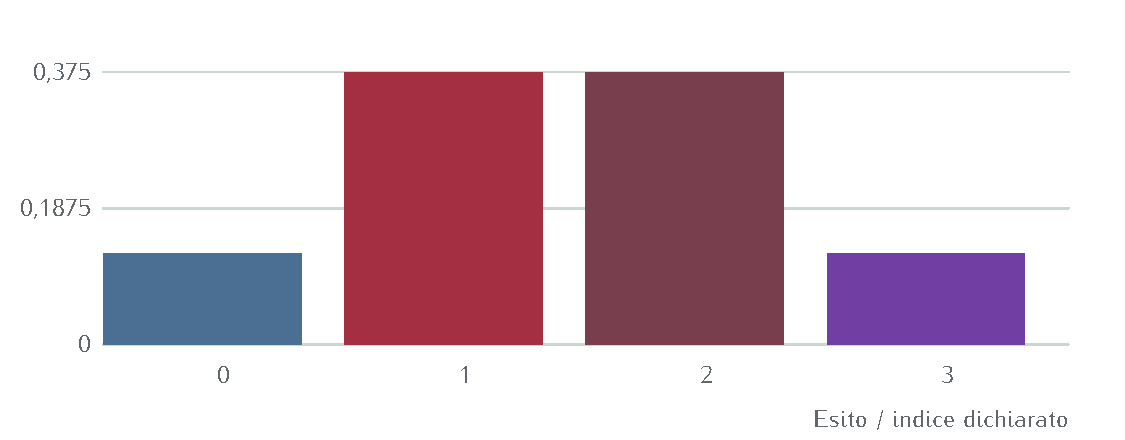
\includegraphics[width=\linewidth,height=94mm,keepaspectratio]{figure/fd021e166b94f8079.pdf}\FigureCaption{2.19 \(\cdot\) esempio 1 \(\cdot\) Distribuzione binomiale teorica di \(K\)}\end{FigureBlock}
\begin{FigureBlock}\centering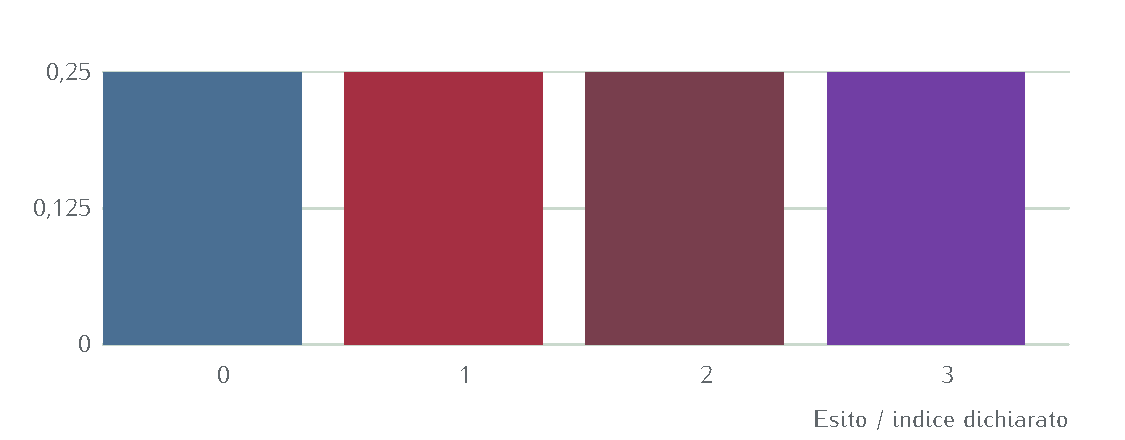
\includegraphics[width=\linewidth,height=94mm,keepaspectratio]{figure/f1af2d87efcdc57a1.pdf}\FigureCaption{2.19 \(\cdot\) esempio 1 \(\cdot\) Frequenze relative delle quattro raccolte dichiarate}\end{FigureBlock}

\phantomsection\label{c2-frequenze-example-1-step-1}
\BookHeading{01 Definire il modello Bernoulli}

\MathBlock{006E003D0033003B0020005000280073007500630063006500730073006F0029003D0070003D0030002E0035003B0020005000280069006E0073007500630063006500730073006F0029003D003122120070003D0030002E0035}{n=3;\allowbreak \ P(\text{successo})=p=0.5;\allowbreak \ P(\text{insuccesso})=1- p=0.5}
\MathBlock{004B003D03A31D62208C2081207F002000581D62003B00200046003D004B002F006E}{K=\sum _{i=1}^{n}\ X_{i};\allowbreak \ F=K/n}

Ogni \(X_{i}\) vale 1 per un successo e 0 altrimenti; le prove sono indipendenti e hanno la stessa probabilità.\par


\phantomsection\label{c2-frequenze-example-1-step-2}
\BookHeading{02 Dichiarare una raccolta illustrativa}

\MathBlock{0052006100630063006F006C0074006100200031003A002000280031002C0030002C00310029003B0020004B003D0032003B00200046003D0032002F003322480030002C0036003600360037}{\text{Raccolta}\ 1:\ (1{,}0{,}1);\allowbreak \ K=2;\allowbreak \ F=2/3\approx 0{,}6667}
\MathBlock{0052006100630063006F006C0074006100200032003A002000280030002C0030002C00300029003B0020004B003D0030003B00200046003D0030002F003322480030}{\text{Raccolta}\ 2:\ (0{,}0{,}0);\allowbreak \ K=0;\allowbreak \ F=0/3\approx 0}
\MathBlock{0052006100630063006F006C0074006100200033003A002000280031002C0031002C00310029003B0020004B003D0033003B00200046003D0033002F003322480031}{\text{Raccolta}\ 3:\ (1{,}1{,}1);\allowbreak \ K=3;\allowbreak \ F=3/3\approx 1}
\MathBlock{0052006100630063006F006C0074006100200034003A002000280030002C0031002C00300029003B0020004B003D0031003B00200046003D0031002F003322480030002C0033003300330033}{\text{Raccolta}\ 4:\ (0{,}1{,}0);\allowbreak \ K=1;\allowbreak \ F=1/3\approx 0{,}3333}

Queste sequenze sono dati illustrativi fissati per il calcolo delle frequenze, non nuove probabilità teoriche e non un campionamento eseguito dal simulatore.\par


\phantomsection\label{c2-frequenze-example-1-step-3}
\BookHeading{03 Costruire l'istogramma delle raccolte}

\MathBlock{004B003D0030003A0020003100200072006100630063006F006C0074006500200073007500200034003B0020006600720065007100750065006E007A0061002000720065006C00610074006900760061003D0031002F0034}{K=0:\ 1\ \text{raccolte}\ \text{su}\ 4;\allowbreak \ \text{frequenza}\ \text{relativa}=1/4}
\MathBlock{004B003D0031003A0020003100200072006100630063006F006C0074006500200073007500200034003B0020006600720065007100750065006E007A0061002000720065006C00610074006900760061003D0031002F0034}{K=1:\ 1\ \text{raccolte}\ \text{su}\ 4;\allowbreak \ \text{frequenza}\ \text{relativa}=1/4}
\MathBlock{004B003D0032003A0020003100200072006100630063006F006C0074006500200073007500200034003B0020006600720065007100750065006E007A0061002000720065006C00610074006900760061003D0031002F0034}{K=2:\ 1\ \text{raccolte}\ \text{su}\ 4;\allowbreak \ \text{frequenza}\ \text{relativa}=1/4}
\MathBlock{004B003D0033003A0020003100200072006100630063006F006C0074006500200073007500200034003B0020006600720065007100750065006E007A0061002000720065006C00610074006900760061003D0031002F0034}{K=3:\ 1\ \text{raccolte}\ \text{su}\ 4;\allowbreak \ \text{frequenza}\ \text{relativa}=1/4}

La frequenza \(F\) entro una raccolta e la frequenza delle raccolte in una classe \(K\) sono due rapporti differenti.\par


\phantomsection\label{c2-frequenze-example-1-step-4}
\BookHeading{04 Contare le sequenze equiprobabili}

\MathBlock{00500028004B003D006A0029003D00430028006E002C006A0029007002B200280031221200700029005E0028006E2212006A0029}{P(K=j)=C(n,\allowbreak j)p^{j}(1- p)^{n- j}}
\MathBlock{00430028006E002C006A0029003D006E0021002F005B006A00210028006E2212006A00290021005D003B002000300021003D0031}{C(n,\allowbreak j)=n!/[j!(n- j)!];\allowbreak \ 0!=1}

Una sequenza con j successi ha probabilità \(p^{j}(1- p)^{n- j}\); il coefficiente binomiale conta le posizioni possibili dei successi.\par


\phantomsection\label{c2-frequenze-example-1-step-5}
\BookHeading{05 Probabilità teorica per \(K=0\)}

\MathBlock{00500028004B003D00300029003D00330021002F005B0030002100B700330021005D00B700280030002E00350029005E003000B700280030002E00350029005E003322480030002C003100320035}{P(K=0)=3!/[0!\cdot 3!]\cdot (0.5)^{0}\cdot (0.5)^{3}\approx 0{,}125}

I possibili conteggi sono n+1, da zero a n inclusi.\par


\phantomsection\label{c2-frequenze-example-1-step-6}
\BookHeading{06 Probabilità teorica per \(K=1\)}

\MathBlock{00500028004B003D00310029003D00330021002F005B0031002100B700320021005D00B700280030002E00350029005E003100B700280030002E00350029005E003222480030002C003300370035}{P(K=1)=3!/[1!\cdot 2!]\cdot (0.5)^{1}\cdot (0.5)^{2}\approx 0{,}375}

I possibili conteggi sono n+1, da zero a n inclusi.\par


\phantomsection\label{c2-frequenze-example-1-step-7}
\BookHeading{07 Probabilità teorica per \(K=2\)}

\MathBlock{00500028004B003D00320029003D00330021002F005B0032002100B700310021005D00B700280030002E00350029005E003200B700280030002E00350029005E003122480030002C003300370035}{P(K=2)=3!/[2!\cdot 1!]\cdot (0.5)^{2}\cdot (0.5)^{1}\approx 0{,}375}

I possibili conteggi sono n+1, da zero a n inclusi.\par


\phantomsection\label{c2-frequenze-example-1-step-8}
\BookHeading{08 Probabilità teorica per \(K=3\)}

\MathBlock{00500028004B003D00330029003D00330021002F005B0033002100B700300021005D00B700280030002E00350029005E003300B700280030002E00350029005E003022480030002C003100320035}{P(K=3)=3!/[3!\cdot 0!]\cdot (0.5)^{3}\cdot (0.5)^{0}\approx 0{,}125}

I possibili conteggi sono n+1, da zero a n inclusi.\par


\phantomsection\label{c2-frequenze-example-1-step-9}
\BookHeading{09 Confrontare media e dispersione}

\MathBlock{0045005B004B005D003D006E0070003D0031002E0035003B00200056006100720028004B0029003D006E007000280031221200700029003D0030002E00370035}{E[K]=np=1.5;\allowbreak \ \operatorname{Var}(K)=np(1- p)=0.75}
\MathBlock{0045005B0046005D003D0070003D0030002E0035003B0020005600610072002800460029003D007000280031221200700029002F006E003D0030002C0030003800330033}{E[F]=p=0.5;\allowbreak \ \operatorname{Var}(F)=p(1- p)/n=0{,}0833}
\MathBlock{004600200063006F006D0070006C0065007300730069007600610020006F00730073006500720076006100740061003D0036002F0031003222480030002C0035}{F\ \text{complessiva}\ \text{osservata}=6/12\approx 0{,}5}

La media teorica descrive molte ripetizioni del modello; una raccolta finita può discostarsene. Con zero raccolte la frequenza relativa non è definita.\par


\BookHeading{Interpretazione}

Le quattro raccolte producono una frequenza relativa 1/4 per ogni classe \(K\), mentre la teoria assegna (1/8,3/8,3/8,1/8). La differenza rende visibili le fluttuazioni finite.\par


\Needspace{.36\textheight}\phantomsection\label{c2-frequenze-example-2}
{\sffamily\small\color{Accent} ESEMPIO SVOLTO 2\par}
\BookHeading{Successo raro, quattro prove per raccolta}
Dati \(n=4\), \(p=0.25\); quattro raccolte illustrative di 4 prove binarie sono elencate nei passaggi.\par


\BookHeading{Geometria e configurazione dell'esempio}
\begin{FigureBlock}\centering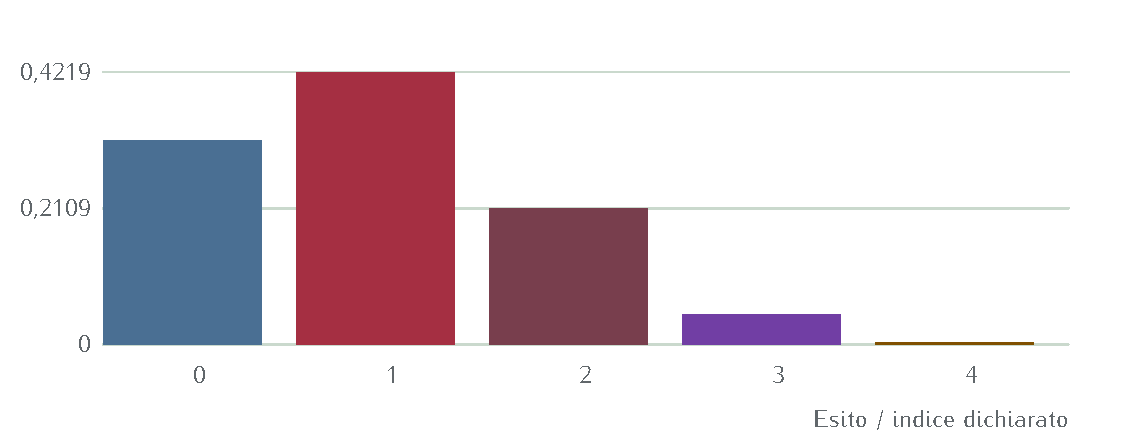
\includegraphics[width=\linewidth,height=94mm,keepaspectratio]{figure/f88e2fd3519c7ab08.pdf}\FigureCaption{2.19 \(\cdot\) esempio 2 \(\cdot\) Distribuzione binomiale teorica di \(K\)}\end{FigureBlock}
\begin{FigureBlock}\centering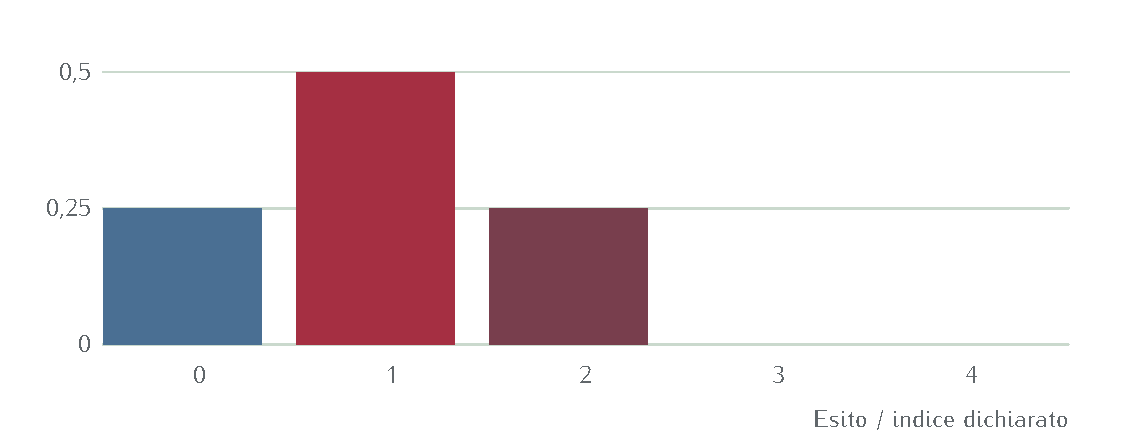
\includegraphics[width=\linewidth,height=94mm,keepaspectratio]{figure/f05a72779686a2fc4.pdf}\FigureCaption{2.19 \(\cdot\) esempio 2 \(\cdot\) Frequenze relative delle quattro raccolte dichiarate}\end{FigureBlock}

\phantomsection\label{c2-frequenze-example-2-step-1}
\BookHeading{01 Definire il modello Bernoulli}

\MathBlock{006E003D0034003B0020005000280073007500630063006500730073006F0029003D0070003D0030002E00320035003B0020005000280069006E0073007500630063006500730073006F0029003D003122120070003D0030002E00370035}{n=4;\allowbreak \ P(\text{successo})=p=0.25;\allowbreak \ P(\text{insuccesso})=1- p=0.75}
\MathBlock{004B003D03A31D62208C2081207F002000581D62003B00200046003D004B002F006E}{K=\sum _{i=1}^{n}\ X_{i};\allowbreak \ F=K/n}

Ogni \(X_{i}\) vale 1 per un successo e 0 altrimenti; le prove sono indipendenti e hanno la stessa probabilità.\par


\phantomsection\label{c2-frequenze-example-2-step-2}
\BookHeading{02 Dichiarare una raccolta illustrativa}

\MathBlock{0052006100630063006F006C0074006100200031003A002000280030002C0030002C0030002C00300029003B0020004B003D0030003B00200046003D0030002F003422480030}{\text{Raccolta}\ 1:\ (0{,}0{,}0{,}0);\allowbreak \ K=0;\allowbreak \ F=0/4\approx 0}
\MathBlock{0052006100630063006F006C0074006100200032003A002000280031002C0030002C0030002C00300029003B0020004B003D0031003B00200046003D0031002F003422480030002C00320035}{\text{Raccolta}\ 2:\ (1{,}0{,}0{,}0);\allowbreak \ K=1;\allowbreak \ F=1/4\approx 0{,}25}
\MathBlock{0052006100630063006F006C0074006100200033003A002000280030002C0031002C0030002C00300029003B0020004B003D0031003B00200046003D0031002F003422480030002C00320035}{\text{Raccolta}\ 3:\ (0{,}1{,}0{,}0);\allowbreak \ K=1;\allowbreak \ F=1/4\approx 0{,}25}
\MathBlock{0052006100630063006F006C0074006100200034003A002000280031002C0030002C0031002C00300029003B0020004B003D0032003B00200046003D0032002F003422480030002C0035}{\text{Raccolta}\ 4:\ (1{,}0{,}1{,}0);\allowbreak \ K=2;\allowbreak \ F=2/4\approx 0{,}5}

Queste sequenze sono dati illustrativi fissati per il calcolo delle frequenze, non nuove probabilità teoriche e non un campionamento eseguito dal simulatore.\par


\phantomsection\label{c2-frequenze-example-2-step-3}
\BookHeading{03 Costruire l'istogramma delle raccolte}

\MathBlock{004B003D0030003A0020003100200072006100630063006F006C0074006500200073007500200034003B0020006600720065007100750065006E007A0061002000720065006C00610074006900760061003D0031002F0034}{K=0:\ 1\ \text{raccolte}\ \text{su}\ 4;\allowbreak \ \text{frequenza}\ \text{relativa}=1/4}
\MathBlock{004B003D0031003A0020003200200072006100630063006F006C0074006500200073007500200034003B0020006600720065007100750065006E007A0061002000720065006C00610074006900760061003D0032002F0034}{K=1:\ 2\ \text{raccolte}\ \text{su}\ 4;\allowbreak \ \text{frequenza}\ \text{relativa}=2/4}
\MathBlock{004B003D0032003A0020003100200072006100630063006F006C0074006500200073007500200034003B0020006600720065007100750065006E007A0061002000720065006C00610074006900760061003D0031002F0034}{K=2:\ 1\ \text{raccolte}\ \text{su}\ 4;\allowbreak \ \text{frequenza}\ \text{relativa}=1/4}
\MathBlock{004B003D0033003A0020003000200072006100630063006F006C0074006500200073007500200034003B0020006600720065007100750065006E007A0061002000720065006C00610074006900760061003D0030002F0034}{K=3:\ 0\ \text{raccolte}\ \text{su}\ 4;\allowbreak \ \text{frequenza}\ \text{relativa}=0/4}
\MathBlock{004B003D0034003A0020003000200072006100630063006F006C0074006500200073007500200034003B0020006600720065007100750065006E007A0061002000720065006C00610074006900760061003D0030002F0034}{K=4:\ 0\ \text{raccolte}\ \text{su}\ 4;\allowbreak \ \text{frequenza}\ \text{relativa}=0/4}

La frequenza \(F\) entro una raccolta e la frequenza delle raccolte in una classe \(K\) sono due rapporti differenti.\par


\phantomsection\label{c2-frequenze-example-2-step-4}
\BookHeading{04 Contare le sequenze equiprobabili}

\MathBlock{00500028004B003D006A0029003D00430028006E002C006A0029007002B200280031221200700029005E0028006E2212006A0029}{P(K=j)=C(n,\allowbreak j)p^{j}(1- p)^{n- j}}
\MathBlock{00430028006E002C006A0029003D006E0021002F005B006A00210028006E2212006A00290021005D003B002000300021003D0031}{C(n,\allowbreak j)=n!/[j!(n- j)!];\allowbreak \ 0!=1}

Una sequenza con j successi ha probabilità \(p^{j}(1- p)^{n- j}\); il coefficiente binomiale conta le posizioni possibili dei successi.\par


\phantomsection\label{c2-frequenze-example-2-step-5}
\BookHeading{05 Probabilità teorica per \(K=0\)}

\MathBlock{00500028004B003D00300029003D00340021002F005B0030002100B700340021005D00B700280030002E003200350029005E003000B700280030002E003700350029005E003422480030002C0033003100360034}{P(K=0)=4!/[0!\cdot 4!]\cdot (0.25)^{0}\cdot (0.75)^{4}\approx 0{,}3164}

I possibili conteggi sono n+1, da zero a n inclusi.\par


\phantomsection\label{c2-frequenze-example-2-step-6}
\BookHeading{06 Probabilità teorica per \(K=1\)}

\MathBlock{00500028004B003D00310029003D00340021002F005B0031002100B700330021005D00B700280030002E003200350029005E003100B700280030002E003700350029005E003322480030002C0034003200310039}{P(K=1)=4!/[1!\cdot 3!]\cdot (0.25)^{1}\cdot (0.75)^{3}\approx 0{,}4219}

I possibili conteggi sono n+1, da zero a n inclusi.\par


\phantomsection\label{c2-frequenze-example-2-step-7}
\BookHeading{07 Probabilità teorica per \(K=2\)}

\MathBlock{00500028004B003D00320029003D00340021002F005B0032002100B700320021005D00B700280030002E003200350029005E003200B700280030002E003700350029005E003222480030002C0032003100300039}{P(K=2)=4!/[2!\cdot 2!]\cdot (0.25)^{2}\cdot (0.75)^{2}\approx 0{,}2109}

I possibili conteggi sono n+1, da zero a n inclusi.\par


\phantomsection\label{c2-frequenze-example-2-step-8}
\BookHeading{08 Probabilità teorica per \(K=3\)}

\MathBlock{00500028004B003D00330029003D00340021002F005B0033002100B700310021005D00B700280030002E003200350029005E003300B700280030002E003700350029005E003122480030002C0030003400360039}{P(K=3)=4!/[3!\cdot 1!]\cdot (0.25)^{3}\cdot (0.75)^{1}\approx 0{,}0469}

I possibili conteggi sono n+1, da zero a n inclusi.\par


\phantomsection\label{c2-frequenze-example-2-step-9}
\BookHeading{09 Probabilità teorica per \(K=4\)}

\MathBlock{00500028004B003D00340029003D00340021002F005B0034002100B700300021005D00B700280030002E003200350029005E003400B700280030002E003700350029005E003022480030002C0030003000330039}{P(K=4)=4!/[4!\cdot 0!]\cdot (0.25)^{4}\cdot (0.75)^{0}\approx 0{,}0039}

I possibili conteggi sono n+1, da zero a n inclusi.\par


\phantomsection\label{c2-frequenze-example-2-step-10}
\BookHeading{10 Confrontare media e dispersione}

\MathBlock{0045005B004B005D003D006E0070003D0031003B00200056006100720028004B0029003D006E007000280031221200700029003D0030002E00370035}{E[K]=np=1;\allowbreak \ \operatorname{Var}(K)=np(1- p)=0.75}
\MathBlock{0045005B0046005D003D0070003D0030002E00320035003B0020005600610072002800460029003D007000280031221200700029002F006E003D0030002C0030003400360039}{E[F]=p=0.25;\allowbreak \ \operatorname{Var}(F)=p(1- p)/n=0{,}0469}
\MathBlock{004600200063006F006D0070006C0065007300730069007600610020006F00730073006500720076006100740061003D0034002F0031003622480030002C00320035}{F\ \text{complessiva}\ \text{osservata}=4/16\approx 0{,}25}

La media teorica descrive molte ripetizioni del modello; una raccolta finita può discostarsene. Con zero raccolte la frequenza relativa non è definita.\par


\BookHeading{Interpretazione}

Le cinque classi teoriche includono \(K=3\) e \(K=4\) anche se le quattro raccolte dichiarate non li contengono. Un conteggio osservato nullo non dimostra probabilità nulla.\par


\Needspace{7\baselineskip}
\BookHeading{Il passaggio successivo}
Le frequenze distinguono dati osservati e modello. Le tabelle congiunte permetteranno ora di aggiornare la distribuzione quando un risultato parziale è noto.\par


\Needspace{.43\textheight}
\section{Selezionare un'informazione}
\phantomsection\label{c2-condizionamento}

{\sffamily\small\color{Ink!70} Riferimento alle slide: p. 264.\par}

{\sffamily\small\color{Ink!70} Laboratorio locale: \nolinkurl{index.html#capitolo-2/condizionamento}\par}

\BookHeading{Definizioni e costruzione}
Una tabella congiunta permette di distinguere i dati completi dalle marginali. Quando selezioniamo un evento di probabilità positiva, rinormalizziamo i pesi rimasti.\par

La probabilità condizionata usa come nuovo insieme di riferimento gli esiti compatibili con l'informazione \(B\). Il peso di \(A\cap B\) viene diviso per P(B), che è il totale degli esiti rimasti. Se \(P(B)=0\), questa formula non definisce una distribuzione condizionata.\par

Da \(P(A\cap B)=P(A|B)P(B)=P(B|A)P(A)\) si ricava la regola di Bayes. Una tabella congiunta permette di leggere tutte queste quantità e le marginali. Il condizionamento descrive un aggiornamento dell'informazione; un rapporto causale richiede ipotesi ulteriori.\par


\MathBlock{005000280041007C00420029003D005000280041222900420029002F0050002800420029002C00200073006500200050002800420029003E0030002E}{P(A|B)=P(A\cap B)/P(B),\allowbreak \ \text{se}\ P(B)>0.}

\BookHeading{Come leggere le figure}
Quattro esiti congiunti; il condizionamento cambia l'insieme di riferimento.\par


\Needspace{.36\textheight}\phantomsection\label{c2-condizionamento-example-1}
{\sffamily\small\color{Accent} ESEMPIO SVOLTO 1\par}
\BookHeading{Marginali e Bayes da una tabella}
Dati pesi congiunti (1,2,3,4) nell'ordine 00,01,10,11.\par


\BookHeading{Geometria e configurazione dell'esempio}
\begin{FigureBlock}\centering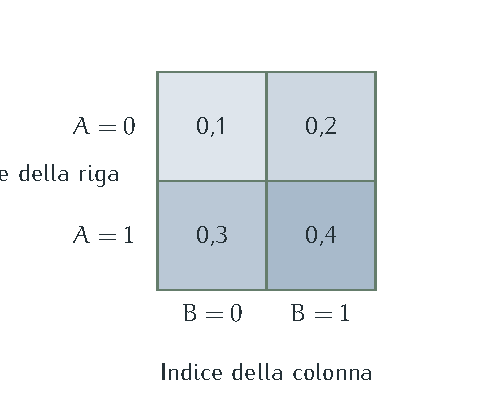
\includegraphics[width=\linewidth,height=94mm,keepaspectratio]{figure/f4e8ed8128e79d075.pdf}\FigureCaption{2.20 \(\cdot\) esempio 1 \(\cdot\) Tabella congiunta \(P(A=a,\allowbreak B=b)\)}\end{FigureBlock}

\phantomsection\label{c2-condizionamento-example-1-step-1}
\BookHeading{01 Normalizzare i pesi}

\MathBlock{0057003D0031002B0032002B0033002B0034003D00310030}{W=1+2+3+4=10}
\MathBlock{0070003D00280031002F00310030002C00200032002F00310030002C00200033002F00310030002C00200034002F003100300029}{p=(1/10,\allowbreak \ 2/10,\allowbreak \ 3/10,\allowbreak \ 4/10)}
\MathBlock{03A30070003D0031}{\sum p=1}

Il totale positivo permette di dividere tutti i pesi per lo stesso numero.\par


\phantomsection\label{c2-condizionamento-example-1-step-2}
\BookHeading{02 Sommare righe e colonne}

\MathBlock{005000280041003D00300029003D0030002C0031002B0030002C0032003D0030002C0033003B0020005000280041003D00310029003D0030002C0037}{P(A=0)=0{,}1+0{,}2=0{,}3;\allowbreak \ P(A=1)=0{,}7}
\MathBlock{005000280042003D00300029003D0030002C0031002B0030002C0033003D0030002C0034003B0020005000280042003D00310029003D0030002C0036}{P(B=0)=0{,}1+0{,}3=0{,}4;\allowbreak \ P(B=1)=0{,}6}

Le somme eliminano l'etichetta del sistema che non si sta descrivendo.\par


\phantomsection\label{c2-condizionamento-example-1-step-3}
\BookHeading{03 Condizionare sulla prima riga}

\MathBlock{005000280042003D0030007C0041003D00300029003D0030002C0031002F0030002C0033003D0030002C0033003300330033}{P(B=0|A=0)=0{,}1/0{,}3=0{,}3333}
\MathBlock{005000280042003D0031007C0041003D00300029003D0030002C0032002F0030002C0033003D0030002C0036003600360037}{P(B=1|A=0)=0{,}2/0{,}3=0{,}6667}

Il denominatore è positivo e i due rapporti sommano a uno.\par


\phantomsection\label{c2-condizionamento-example-1-step-4}
\BookHeading{04 Invertire il condizionamento con Bayes}

\MathBlock{005000280041003D0030007C0042003D00300029003D005000280042003D0030007C0041003D00300029005000280041003D00300029002F005000280042003D00300029}{P(A=0|B=0)=P(B=0|A=0)P(A=0)/P(B=0)}
\MathBlock{003D0030002C003300330033003300B70030002C0033002F0030002C0034003D0030002C00320035}{=0{,}3333\cdot 0{,}3/0{,}4=0{,}25}

L'intersezione è la stessa cella \(P_{00}\); cambia l'insieme usato come riferimento.\par


\BookHeading{Interpretazione}

La marginale \(P(B=0)=0{,}4\) diventa \(P(B=0|A=0)=1/3\): selezionare una riga cambia il totale di riferimento.\par


\Needspace{.36\textheight}\phantomsection\label{c2-condizionamento-example-2}
{\sffamily\small\color{Accent} ESEMPIO SVOLTO 2\par}
\BookHeading{Correlazione perfetta e condizione impossibile}
Dati \(P_{00}=P_{11}=1/2\) e \(P_{01}=P_{10}=0\).\par


\BookHeading{Geometria e configurazione dell'esempio}
\begin{FigureBlock}\centering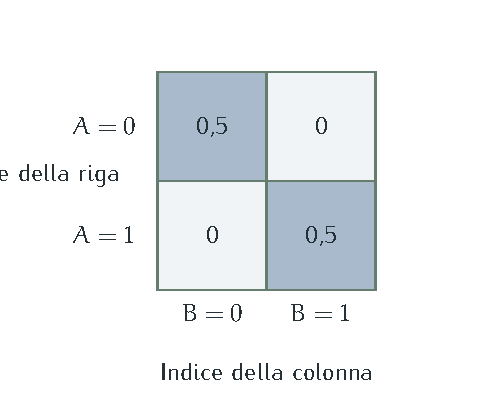
\includegraphics[width=\linewidth,height=94mm,keepaspectratio]{figure/fa5c834a1d06046c8.pdf}\FigureCaption{2.20 \(\cdot\) esempio 2 \(\cdot\) Tabella congiunta \(P(A=a,\allowbreak B=b)\)}\end{FigureBlock}

\phantomsection\label{c2-condizionamento-example-2-step-1}
\BookHeading{01 Dichiarare la congiunta}

\MathBlock{005000300030003D0031002F0032003B0020005000300031003D0030003B0020005000310030003D0030003B0020005000310031003D0031002F0032003B002003A3005000610062003D0031}{P_{00}=1/2;\allowbreak \ P_{01}=0;\allowbreak \ P_{10}=0;\allowbreak \ P_{11}=1/2;\allowbreak \ \sum \text{Pab}=1}

Le due etichette della coppia indicano nell'ordine riga \(A\) e colonna \(B\).\par


\phantomsection\label{c2-condizionamento-example-2-step-2}
\BookHeading{02 Sommare righe e colonne}

\MathBlock{005000280041003D00300029003D0030002C0035002B0030003D0030002C0035003B0020005000280041003D00310029003D0030002C0035}{P(A=0)=0{,}5+0=0{,}5;\allowbreak \ P(A=1)=0{,}5}
\MathBlock{005000280042003D00300029003D0030002C0035002B0030003D0030002C0035003B0020005000280042003D00310029003D0030002C0035}{P(B=0)=0{,}5+0=0{,}5;\allowbreak \ P(B=1)=0{,}5}

Le somme eliminano l'etichetta del sistema che non si sta descrivendo.\par


\phantomsection\label{c2-condizionamento-example-2-step-3}
\BookHeading{03 Condizionare sulla prima riga}

\MathBlock{005000280042003D0030007C0041003D00300029003D0030002C0035002F0030002C0035003D0031}{P(B=0|A=0)=0{,}5/0{,}5=1}
\MathBlock{005000280042003D0031007C0041003D00300029003D0030002F0030002C0035003D0030}{P(B=1|A=0)=0/0{,}5=0}

Il denominatore è positivo e i due rapporti sommano a uno.\par


\phantomsection\label{c2-condizionamento-example-2-step-4}
\BookHeading{04 Invertire il condizionamento con Bayes}

\MathBlock{005000280041003D0030007C0042003D00300029003D005000280042003D0030007C0041003D00300029005000280041003D00300029002F005000280042003D00300029}{P(A=0|B=0)=P(B=0|A=0)P(A=0)/P(B=0)}
\MathBlock{003D003100B70030002C0035002F0030002C0035003D0031}{=1\cdot 0{,}5/0{,}5=1}

L'intersezione è la stessa cella \(P_{00}\); cambia l'insieme usato come riferimento.\par


\phantomsection\label{c2-condizionamento-example-2-step-5}
\BookHeading{05 Trattare un'informazione impossibile}

\MathBlock{0045003D007B004122600042007D003B00200050002800450029003D005000300031002B005000310030003D0030}{E=\{A\ne B\};\allowbreak \ P(E)=P_{01}+P_{10}=0}
\MathBlock{005000280041003D0030007C00450029003D005000280041003D0030002000650064002000450029002F0050002800450029003D0030002F00300020006E006F006E00200064006500660069006E00690074006F}{P(A=0|E)=P(A=0\ ed\ E)/P(E)=0/0\ \text{non}\ \text{definito}}

Un evento nullo non permette di costruire una distribuzione condizionata mediante questa formula.\par


\BookHeading{Interpretazione}

Sapere \(A=0\) rende \(B=0\) certo. Selezionare \(A\ne B\) è impossibile nel modello e il rapporto condizionato non è definito.\par


\Needspace{7\baselineskip}
\BookHeading{Il passaggio successivo}
La selezione di un evento richiede un peso positivo. Nella misura quantistica ritroveremo questa rinormalizzazione dopo aver costruito le ampiezze dello stato.\par


% Authoritative exercise source. Preserve all derivations and diagrams.

\ExerciseStart{G2.11}{Dagli eventi a media e varianza}{Collegamento}

\BookHeading{Problema, dati e obiettivo}

Una variabile X assume valori 0, 1, 2 con pesi rispettivamente 1, 2, 1. Normalizzare, calcolare media e varianza, raggruppare gli esiti per parità e condizionare all’evento \(X\geq1\). Confrontare con un campione di 40 prove avente conteggi 9, 22, 9.

\ExTheory{\ExRef{c2-eventi}{2.16}; \ExRef{c2-distribuzioni}{2.17}; \ExRef{c2-momenti}{2.18}; \ExRef{c2-frequenze}{2.19}; \ExRef{c2-condizionamento}{2.20}}{Pesi non negativi \(w_j\) si normalizzano mediante \(p_j=w_j/\sum_kw_k\). I momenti sono \(\mathbb E[X]=\sum_jx_jp_j\) ed \(\mathbb E[X^2]=\sum_jx_j^2p_j\); la varianza è \(\mathbb E[X^2]-\mathbb E[X]^2\). Il condizionamento divide i pesi dell’evento per la sua probabilità.}

\ExPrediction{La distribuzione è simmetrica attorno a 1. La media dovrebbe coincidere con il centro, mentre il condizionamento che esclude zero dovrebbe spostarla verso destra.}

\ExFigure{\begin{tikzpicture}[>=Stealth,exlabel]
\draw[exaxis] (-.6,0)--(3.3000000000000003,0) node[right] {esito};\draw[exaxis] (-.6,0)--(-.6,3.6) node[above] {$w$};\node[left] at (-.6,3) {$ 2 $};\draw[Ink!15,dashed] (-.6,3)--(2.8000000000000003,3);\filldraw[fill=Accent!25,draw=Accent] (0.0,0) rectangle (0.65,1.5);\node[below] at (0.325,0) {$ 0 $};\node[above] at (0.325,1.5) {$ 1 $};\filldraw[fill=Accent!25,draw=Accent] (1.1,0) rectangle (1.75,3.0);\node[below] at (1.425,0) {$ 1 $};\node[above] at (1.425,3.0) {$ 2 $};\filldraw[fill=Accent!25,draw=Accent] (2.2,0) rectangle (2.85,1.5);\node[below] at (2.5250000000000004,0) {$ 2 $};\node[above] at (2.5250000000000004,1.5) {$ 1 $};
\end{tikzpicture}}{Pesi iniziali: l’asse verticale indica \(w_j\), prima della normalizzazione.}


\begin{ExTasks}

\item Calcolare il peso totale e le probabilità.

\item Calcolare separatamente primo e secondo momento.

\item Ricavare la varianza.

\item Raggruppare per parità e condizionare a \(X\geq1\).

\item Calcolare le frequenze campionarie e distinguerle dalle probabilità.

\end{ExTasks}

\ExSolution

\ExStep{Normalizzare}

Il totale è \(W=1+2+1=4\), dunque \(p=(1/4,1/2,1/4)\). La somma \(1/4+1/2+1/4=1\) controlla la normalizzazione.

\ExStep{Calcolare i momenti}

\ExEq{\mathbb E[X]&=0\cdot\tfrac14+1\cdot\tfrac12+2\cdot\tfrac14=1,\\\mathbb E[X^2]&=0^2\cdot\tfrac14+1^2\cdot\tfrac12+2^2\cdot\tfrac14
=\tfrac12+1=\tfrac32.}

\ExStep{Calcolare la dispersione}

\ExEq{\operatorname{Var}(X)&=\tfrac32-1^2=\tfrac12.}
Il calcolo diretto conferma \((0-1)^2/4+(1-1)^2/2+(2-1)^2/4=1/2\).

\ExStep{Raggruppare gli esiti}

Gli esiti pari sono 0 e 2: \(P(\mathrm{pari})=1/4+1/4=1/2\). L’esito dispari è 1: \(P(\mathrm{dispari})=1/2\). Il raggruppamento somma probabilità di eventi disgiunti.

\ExStep{Condizionare}

\ExEq{P(X\geq1)&=1/2+1/4=3/4,\\P(1\mid X\geq1)&=(1/2)/(3/4)=2/3,\\P(2\mid X\geq1)&=(1/4)/(3/4)=1/3,\\\mathbb E[X\mid X\geq1]&=1\cdot2/3+2\cdot1/3=4/3.}

\ExStep{Leggere un campione finito}

I conteggi sommano \(9+22+9=40\). Le frequenze sono \(9/40=0{,}225\), \(22/40=0{,}55\), \(9/40=0{,}225\). I conteggi medi teorici erano \((10,20,10)\). La media empirica è \((0\cdot9+22+2\cdot9)/40=1\); la varianza con divisore 40 è \((9+9)/40=0{,}45\).

\par\noindent\begin{minipage}{\linewidth}
\ExFigure{\begin{tikzpicture}[>=Stealth,exlabel]
\draw[exaxis] (-.6,0)--(3.3000000000000003,0) node[right] {esito};\draw[exaxis] (-.6,0)--(-.6,3.6) node[above] {$p$};\node[left] at (-.6,3) {$ 1 $};\draw[Ink!15,dashed] (-.6,3)--(2.8000000000000003,3);\filldraw[fill=Accent!25,draw=Accent] (0.0,0) rectangle (0.65,0.75);\node[below] at (0.325,0) {$ 0 $};\node[above] at (0.325,0.75) {$ 0.25 $};\filldraw[fill=Accent!25,draw=Accent] (1.1,0) rectangle (1.75,1.5);\node[below] at (1.425,0) {$ 1 $};\node[above] at (1.425,1.5) {$ 0.5 $};\filldraw[fill=Accent!25,draw=Accent] (2.2,0) rectangle (2.85,0.75);\node[below] at (2.5250000000000004,0) {$ 2 $};\node[above] at (2.5250000000000004,0.75) {$ 0.25 $};
\end{tikzpicture}}{Probabilità normalizzate. La simmetria intorno a 1 determina la media.}


\ExInterpret{Probabilità, frequenze e distribuzioni condizionate rispondono a domande diverse. Nel campione la media può coincidere con quella teorica mentre la dispersione differisce.}

\ExLab{Nelle sezioni 2.16–2.20 ripercorrere normalizzazione, raggruppamento, momenti e condizionamento. Usare i dati dell’esercizio come tabella di controllo e confrontare un campione simulato con i conteggi medi, mantenendo distinti valore atteso e realizzazione osservata.}


\end{minipage}

\Needspace{.43\textheight}
\section{Preparare un vettore di stato}
\phantomsection\label{c2-stati}

{\sffamily\small\color{Ink!70} Riferimento alle slide: p. 319.\par}

{\sffamily\small\color{Ink!70} Laboratorio locale: \nolinkurl{index.html#capitolo-2/stati}\par}

\BookHeading{Definizioni e costruzione}
Le due ampiezze di un qubit devono avere norma quadra totale uno. La normalizzazione permette di usare i loro moduli quadri come probabilità nella base assegnata.\par

Fissiamo la base ortonormale \(|0\rangle =(1{,}0)^{T}\) e \(|1\rangle =(0{,}1)^{T}\). La scrittura \(|\psi \rangle \), detta ket, indica il vettore colonna \(\psi =\alpha |0\rangle +\beta |1\rangle \) in \(C^{2}\). Un qubit puro richiede \(|\alpha |^{2}+|\beta |^{2}=1\); nella misura di questa base i moduli quadri danno le probabilità di 0 e 1. Una fase globale \(e^{i\gamma }\) comune alle due componenti lascia invariata la preparazione fisica.\par

Per costruire la sfera di Bloch usiamo tre quantità invarianti sotto quella fase comune: \(r_{x}=2\operatorname{Re}(\alpha {}^{*}\beta )\), \(r_{y}=2\operatorname{Im}(\alpha {}^{*}\beta )\), \(r_{z}=|\alpha |^{2}- |\beta |^{2}\). La loro norma quadra è \(4|\alpha |^{2}|\beta |^{2}+(|\alpha |^{2}- |\beta |^{2})^{2}=(|\alpha |^{2}+|\beta |^{2})^{2}=1\). Si ottiene quindi un punto della sfera unitaria. Gli assi sono coordinate adimensionali dello stato: +Z e \(- Z\) rappresentano \(|0\rangle \) e \(|1\rangle \), +X rappresenta \((1{,}1)/\sqrt{2}\) e +Y rappresenta \((1,\allowbreak i)/\sqrt{2}\). La sfera non raffigura l'apparato nello spazio fisico.\par

Dopo aver eliminato la fase globale, si può scrivere \(\alpha =\cos (\theta /2)\), \(\beta =e^{i\varphi }\sin (\theta /2)\), con \(0\le \theta \le \pi \). Infatti \(r_{z}=\cos ^{2}(\theta /2)- \sin ^{2}(\theta /2)=\cos \theta \) e \(\alpha {}^{*}\beta =(1/2)e^{i\varphi }\sin \theta \), perciò \(r=(\sin \theta \) \(\cos \varphi ,\allowbreak \sin \theta \) \(\sin \varphi ,\allowbreak \cos \theta )\). L'angolo polare di Bloch è \(\theta \); la fase relativa è \(\varphi \). Ai poli \(\varphi \) è irrilevante. Il mezzo angolo nasce dalle identità dei quadrati di seno e coseno.\par

Lo stato \(\chi =(- \beta {}^{*},\allowbreak \alpha {}^{*})^{T}\) è normalizzato e ortogonale a \(\psi \), poiché \(\langle \psi ,\allowbreak \chi \rangle =- \alpha {}^{*}\beta {}^{*}+\beta {}^{*}\alpha {}^{*}=0\). Inserendone le componenti nella stessa mappa si trova \(r\chi =- r\psi \): gli stati ortogonali sono antipodali. Il valore \(P(0)=|\alpha |^{2}=(1+r_{z})/2\) si legge direttamente dalla coordinata verticale. Un angolo retto fra due punti di Bloch avrà invece probabilità di sovrapposizione 1/2, come verrà ricavato nella misura proiettiva.\par


\MathBlock{007C03C827E9003D03B1007C003027E9002B03B2007C003127E9003B0020007C03B1007C00B2002B007C03B2007C00B2003D0031002E}{|\psi \rangle =\alpha |0\rangle +\beta |1\rangle ;\allowbreak \ |\alpha |^{2}+|\beta |^{2}=1.}

\BookHeading{Come leggere le figure}
Due piani complessi per le componenti di \(C^{2}\); nessun piano coincide con lo spazio fisico.\par


\Needspace{.36\textheight}\phantomsection\label{c2-stati-example-1}
{\sffamily\small\color{Accent} ESEMPIO SVOLTO 1\par}
\BookHeading{Dalle ampiezze alla latitudine di Bloch}
Dati \(\psi \) \(\text{grezzo}=(2,\allowbreak i)^{T}\) e base computazionale \(|0\rangle =(1{,}0)^{T}\), \(|1\rangle =(0{,}1)^{T}\).\par


\BookHeading{Geometria e configurazione dell'esempio}
\begin{FigureBlock}\begin{minipage}[t]{.485\linewidth}\centering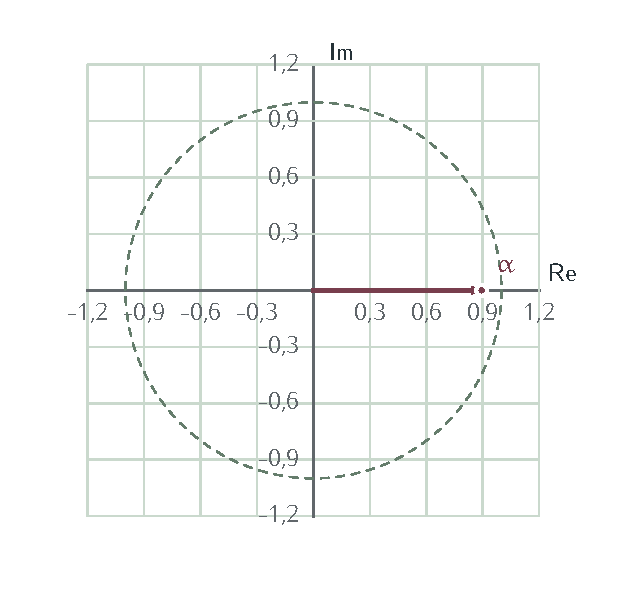
\includegraphics[width=\linewidth,height=63mm,keepaspectratio]{figure/f58bb14f3463ee836.pdf}\par{\sffamily\footnotesize \(\alpha \)\par}\end{minipage}\hfill\begin{minipage}[t]{.485\linewidth}\centering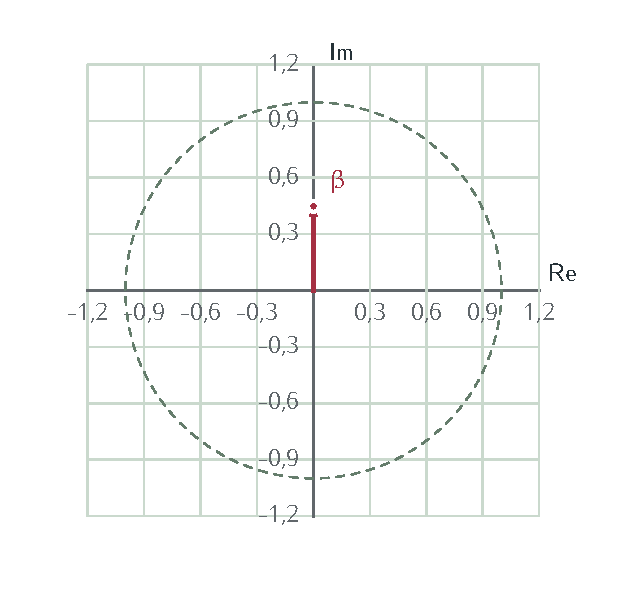
\includegraphics[width=\linewidth,height=63mm,keepaspectratio]{figure/f4551412e5d7210c3.pdf}\par{\sffamily\footnotesize \(\beta \)\par}\end{minipage}\FigureCaption{2.21 \(\cdot\) esempio 1 \(\cdot\) Componenti del ket normalizzato}\end{FigureBlock}
\begin{FigureBlock}\centering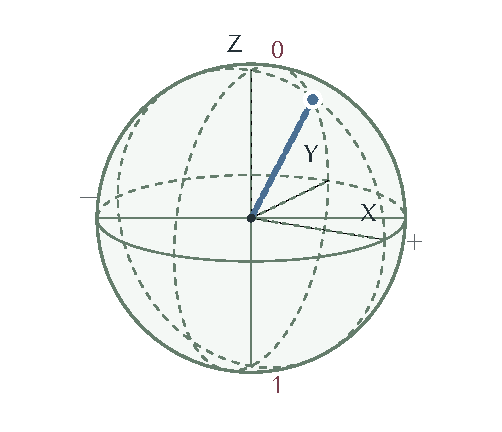
\includegraphics[width=\linewidth,height=94mm,keepaspectratio]{figure/fe3587a4d3c7cb4d0.pdf}\FigureCaption{2.21 \(\cdot\) esempio 1 \(\cdot\) Sfera di Bloch \(\cdot\) stato dell'esempio}\end{FigureBlock}

\phantomsection\label{c2-stati-example-1-step-1}
\BookHeading{01 Normalizzare il dato}

\MathBlock{201600280032002C006900291D40201600B2003D003200B2002B007C0069007C00B2003D0035}{\Vert (2,\allowbreak i)^{T}\Vert ^{2}=2^{2}+|i|^{2}=5}
\MathBlock{03C8003D00280032002C006900291D40002F221A0035003B002003B1003D0032002F221A0035003B002003B2003D0069002F221A0035}{\psi =(2,\allowbreak i)^{T}/\sqrt{5};\allowbreak \ \alpha =2/\sqrt{5};\allowbreak \ \beta =i/\sqrt{5}}

I coefficienti sono riferiti alla base \(|0\rangle =(1{,}0)^{T}\), \(|1\rangle =(0{,}1)^{T}\).\par


\phantomsection\label{c2-stati-example-1-step-2}
\BookHeading{02 Interpretare i moduli quadri}

\MathBlock{007C03B1007C00B2003D0034002F0035003B0020007C03B2007C00B2003D0031002F0035003B0020007C03B1007C00B2002B007C03B2007C00B2003D0031}{|\alpha |^{2}=4/5;\allowbreak \ |\beta |^{2}=1/5;\allowbreak \ |\alpha |^{2}+|\beta |^{2}=1}

Per una misura nella base dichiarata, i due moduli quadri sono le probabilità degli esiti 0 e 1. La regola generale per altre basi verrà costruita con i proiettori.\par


\phantomsection\label{c2-stati-example-1-step-3}
\BookHeading{03 Eliminare una fase comune}

\MathBlock{006903C8003D002800320069002C2212003100291D40002F221A0035}{i\psi =(2i,\allowbreak - 1)^{T}/\sqrt{5}}
\MathBlock{0028006903B10029002A0028006903B20029003D03B1002A03B2003B0020007C006903B1007C00B2003D007C03B1007C00B2003B0020007C006903B2007C00B2003D007C03B2007C00B2}{(i\alpha ){}^{*}(i\beta )=\alpha {}^{*}\beta ;\allowbreak \ |i\alpha |^{2}=|\alpha |^{2};\allowbreak \ |i\beta |^{2}=|\beta |^{2}}

Le quantità usate per descrivere lo stato sono invarianti sotto una fase globale.\par


\phantomsection\label{c2-stati-example-1-step-4}
\BookHeading{04 Costruire le coordinate di Bloch}

\MathBlock{03B1002A03B2003D00320069002F0035}{\alpha {}^{*}\beta =2i/5}
\MathBlock{00722093003D003200520065002803B1002A03B20029003D0030003B002000721D67003D00320049006D002803B1002A03B20029003D0034002F0035003B00200072D835DCCF003D007C03B1007C00B22212007C03B2007C00B2003D0033002F0035}{r_{x}=2\operatorname{Re}(\alpha {}^{*}\beta )=0;\allowbreak \ r_{y}=2\operatorname{Im}(\alpha {}^{*}\beta )=4/5;\allowbreak \ r_{z}=|\alpha |^{2}- |\beta |^{2}=3/5}
\MathBlock{0072003D00280030003B00200030002C0038003B00200030002C00360029003B002020160072201600B2003D00280034002F0035002900B2002B00280033002F0035002900B2003D0031}{r=(0;\allowbreak \ 0{,}8;\allowbreak \ 0{,}6);\allowbreak \ \Vert r\Vert ^{2}=(4/5)^{2}+(3/5)^{2}=1}

La sfera è ottenuta dalle ampiezze e identifica vettori che differiscono per una fase globale. Le sue coordinate sono adimensionali.\par


\phantomsection\label{c2-stati-example-1-step-5}
\BookHeading{05 Ricavare mezzo angolo e probabilità}

\MathBlock{0063006F0073002003B8003D0072D835DCCF003D0033002F0035003B002003B8224800350033002C003100330030003100B0003B002003C6003D0039003000B0}{\cos \ \theta =r_{z}=3/5;\allowbreak \ \theta \approx 53{,}1301{}^{\circ} ;\allowbreak \ \varphi =90{}^{\circ} }
\MathBlock{007C03B1007C003D0063006F0073002803B8002F00320029003B0020007C03B2007C003D00730069006E002803B8002F00320029}{|\alpha |=\cos (\theta /2);\allowbreak \ |\beta |=\sin (\theta /2)}
\MathBlock{0050002800300029003D00280031002B0072D835DCCF0029002F0032003D0034002F0035}{P(0)=(1+r_{z})/2=4/5}

L'identità \(\cos ^{2}(\theta /2)=(1+\cos \) \(\theta )/2\) spiega il mezzo angolo. \(\theta \) è un angolo sulla sfera di Bloch, non la fase relativa \(\varphi \).\par


\BookHeading{Interpretazione}

Le ampiezze \((2,\allowbreak i)/\sqrt{5}\) producono \(r=(0{,}4/5{,}3/5)\); il valore \(r_{z}=3/5\) restituisce \(P(0)=4/5\). La fase globale comune lascia invariato questo punto.\par


\Needspace{.36\textheight}\phantomsection\label{c2-stati-example-2}
{\sffamily\small\color{Accent} ESEMPIO SVOLTO 2\par}
\BookHeading{Stato equatoriale con fase \(\pi /2\)}
Dati \(\psi \) \(\text{grezzo}=(1,\allowbreak i)^{T}\) e base computazionale \(|0\rangle =(1{,}0)^{T}\), \(|1\rangle =(0{,}1)^{T}\).\par


\BookHeading{Geometria e configurazione dell'esempio}
\begin{FigureBlock}\begin{minipage}[t]{.485\linewidth}\centering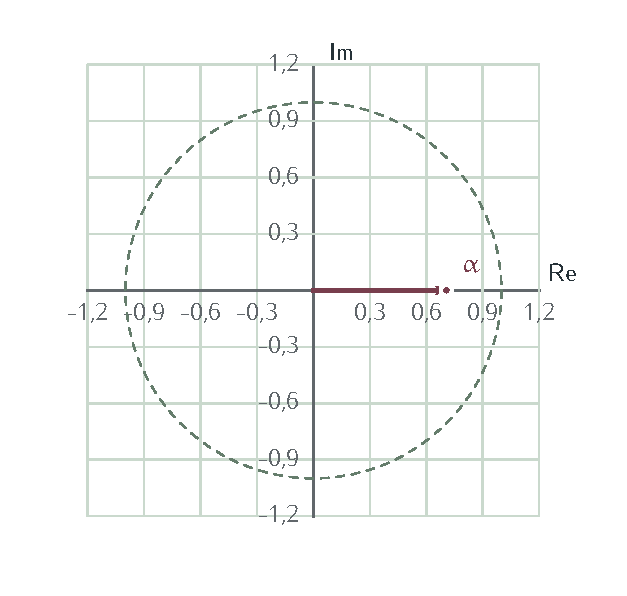
\includegraphics[width=\linewidth,height=63mm,keepaspectratio]{figure/fd88de13169590779.pdf}\par{\sffamily\footnotesize \(\alpha \)\par}\end{minipage}\hfill\begin{minipage}[t]{.485\linewidth}\centering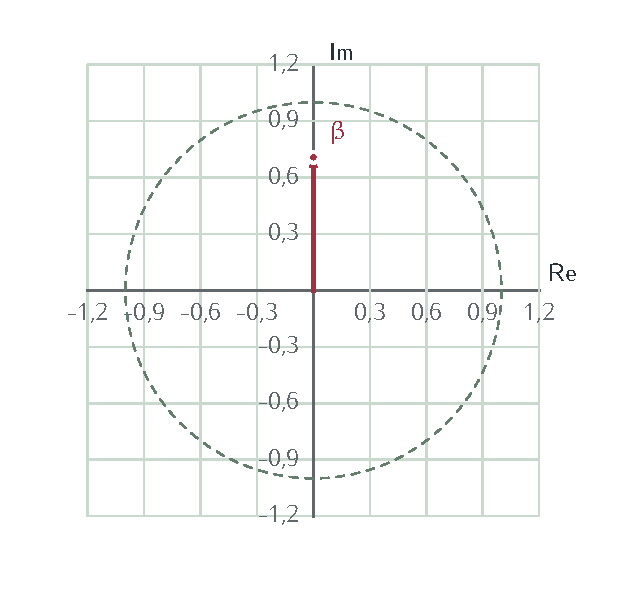
\includegraphics[width=\linewidth,height=63mm,keepaspectratio]{figure/fb7576a3f3d8ba6ee.pdf}\par{\sffamily\footnotesize \(\beta \)\par}\end{minipage}\FigureCaption{2.21 \(\cdot\) esempio 2 \(\cdot\) Componenti del ket normalizzato}\end{FigureBlock}
\begin{FigureBlock}\centering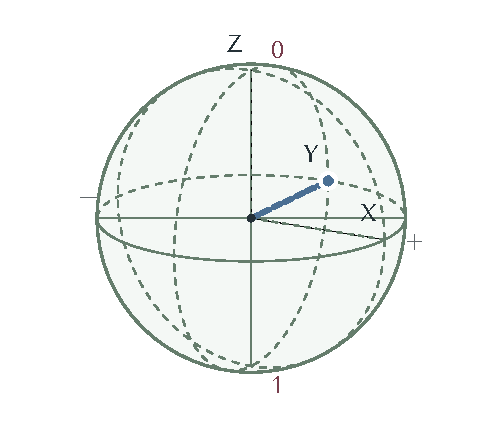
\includegraphics[width=\linewidth,height=94mm,keepaspectratio]{figure/fae21600cc1d0968b.pdf}\FigureCaption{2.21 \(\cdot\) esempio 2 \(\cdot\) Sfera di Bloch \(\cdot\) stato dell'esempio}\end{FigureBlock}

\phantomsection\label{c2-stati-example-2-step-1}
\BookHeading{01 Normalizzare il dato}

\MathBlock{201600280031002C006900291D40201600B2003D003100B2002B007C0069007C00B2003D0032}{\Vert (1,\allowbreak i)^{T}\Vert ^{2}=1^{2}+|i|^{2}=2}
\MathBlock{03C8003D00280031002C006900291D40002F221A0032003B002003B1003D0031002F221A0032003B002003B2003D0069002F221A0032}{\psi =(1,\allowbreak i)^{T}/\sqrt{2};\allowbreak \ \alpha =1/\sqrt{2};\allowbreak \ \beta =i/\sqrt{2}}

I coefficienti sono riferiti alla base \(|0\rangle =(1{,}0)^{T}\), \(|1\rangle =(0{,}1)^{T}\).\par


\phantomsection\label{c2-stati-example-2-step-2}
\BookHeading{02 Interpretare i moduli quadri}

\MathBlock{007C03B1007C00B2003D0031002F0032003B0020007C03B2007C00B2003D0031002F0032003B0020007C03B1007C00B2002B007C03B2007C00B2003D0031}{|\alpha |^{2}=1/2;\allowbreak \ |\beta |^{2}=1/2;\allowbreak \ |\alpha |^{2}+|\beta |^{2}=1}

Per una misura nella base dichiarata, i due moduli quadri sono le probabilità degli esiti 0 e 1. La regola generale per altre basi verrà costruita con i proiettori.\par


\phantomsection\label{c2-stati-example-2-step-3}
\BookHeading{03 Eliminare una fase comune}

\MathBlock{006903C8003D002800310069002C2212003100291D40002F221A0032}{i\psi =(1i,\allowbreak - 1)^{T}/\sqrt{2}}
\MathBlock{0028006903B10029002A0028006903B20029003D03B1002A03B2003B0020007C006903B1007C00B2003D007C03B1007C00B2003B0020007C006903B2007C00B2003D007C03B2007C00B2}{(i\alpha ){}^{*}(i\beta )=\alpha {}^{*}\beta ;\allowbreak \ |i\alpha |^{2}=|\alpha |^{2};\allowbreak \ |i\beta |^{2}=|\beta |^{2}}

Le quantità usate per descrivere lo stato sono invarianti sotto una fase globale.\par


\phantomsection\label{c2-stati-example-2-step-4}
\BookHeading{04 Costruire le coordinate di Bloch}

\MathBlock{03B1002A03B2003D00310069002F0032}{\alpha {}^{*}\beta =1i/2}
\MathBlock{00722093003D003200520065002803B1002A03B20029003D0030003B002000721D67003D00320049006D002803B1002A03B20029003D0032002F0032003B00200072D835DCCF003D007C03B1007C00B22212007C03B2007C00B2003D0030002F0032}{r_{x}=2\operatorname{Re}(\alpha {}^{*}\beta )=0;\allowbreak \ r_{y}=2\operatorname{Im}(\alpha {}^{*}\beta )=2/2;\allowbreak \ r_{z}=|\alpha |^{2}- |\beta |^{2}=0/2}
\MathBlock{0072003D00280030003B00200031003B002000300029003B002020160072201600B2003D00280032002F0032002900B2002B00280030002F0032002900B2003D0031}{r=(0;\allowbreak \ 1;\allowbreak \ 0);\allowbreak \ \Vert r\Vert ^{2}=(2/2)^{2}+(0/2)^{2}=1}

La sfera è ottenuta dalle ampiezze e identifica vettori che differiscono per una fase globale. Le sue coordinate sono adimensionali.\par


\phantomsection\label{c2-stati-example-2-step-5}
\BookHeading{05 Ricavare mezzo angolo e probabilità}

\MathBlock{0063006F0073002003B8003D0072D835DCCF003D0030002F0032003B002003B822480039003000B0003B002003C6003D0039003000B0}{\cos \ \theta =r_{z}=0/2;\allowbreak \ \theta \approx 90{}^{\circ} ;\allowbreak \ \varphi =90{}^{\circ} }
\MathBlock{007C03B1007C003D0063006F0073002803B8002F00320029003B0020007C03B2007C003D00730069006E002803B8002F00320029}{|\alpha |=\cos (\theta /2);\allowbreak \ |\beta |=\sin (\theta /2)}
\MathBlock{0050002800300029003D00280031002B0072D835DCCF0029002F0032003D0031002F0032}{P(0)=(1+r_{z})/2=1/2}

L'identità \(\cos ^{2}(\theta /2)=(1+\cos \) \(\theta )/2\) spiega il mezzo angolo. \(\theta \) è un angolo sulla sfera di Bloch, non la fase relativa \(\varphi \).\par


\BookHeading{Interpretazione}

I moduli uguali collocano lo stato sull'equatore; la fase relativa \(\pi /2\) sceglie il punto +Y. La misura \(Z\) dà probabilità 1/2 a entrambi gli esiti.\par


\Needspace{7\baselineskip}
\BookHeading{Il passaggio successivo}
Le componenti normalizzate e la loro mappa di Bloch descrivono un qubit puro. Il passaggio dal ket al bra renderà espliciti i prodotti interni con altre preparazioni.\par


\Needspace{.43\textheight}
\section{Dal ket al bra}
\phantomsection\label{c2-bra}

{\sffamily\small\color{Ink!70} Riferimento alle slide: p. 331.\par}

{\sffamily\small\color{Ink!70} Laboratorio locale: \nolinkurl{index.html#capitolo-2/bra}\par}

\BookHeading{Definizioni e costruzione}
Il bra è il vettore riga coniugato del ket. Questa operazione rende esplicito il prodotto interno necessario per calcolare ampiezze di misura.\par

Il ket è scritto come vettore colonna. Il bra corrispondente è la riga trasposta e coniugata: ciascun termine x+iy diventa \(x- iy\). La moltiplicazione riga-colonna produce uno scalare complesso, che è il prodotto interno.\par

Il prodotto \(\langle \psi |\psi \rangle \) restituisce la norma quadra. Il prodotto nell'ordine opposto, \(|\psi \rangle \langle \psi |\), è una matrice e descrive un proiettore quando \(\psi \) è normalizzato. La posizione dei simboli rende quindi leggibile anche il tipo dell'oggetto ottenuto dal calcolo.\par


\MathBlock{002803B1002C03B200291D40002021A60020002803B1002A002C03B2002A0029003B002027E803C8007C03C827E9003D007C03B1007C00B2002B007C03B2007C00B2002E}{(\alpha ,\allowbreak \beta )^{T}\ \mapsto \ (\alpha {}^{*},\allowbreak \beta {}^{*});\allowbreak \ \langle \psi |\psi \rangle =|\alpha |^{2}+|\beta |^{2}.}

\BookHeading{Come leggere le figure}
Componenti complesse; il coniugio cambia il segno della parte immaginaria.\par


\Needspace{.36\textheight}\phantomsection\label{c2-bra-example-1}
{\sffamily\small\color{Accent} ESEMPIO SVOLTO 1\par}
\BookHeading{Bra e proiettore sullo stato assegnato}
Dati \(\psi \) \(\text{grezzo}=(2,\allowbreak i)^{T}\) e base computazionale \(|0\rangle =(1{,}0)^{T}\), \(|1\rangle =(0{,}1)^{T}\).\par


\BookHeading{Geometria e configurazione dell'esempio}
\begin{FigureBlock}\begin{minipage}[t]{.485\linewidth}\centering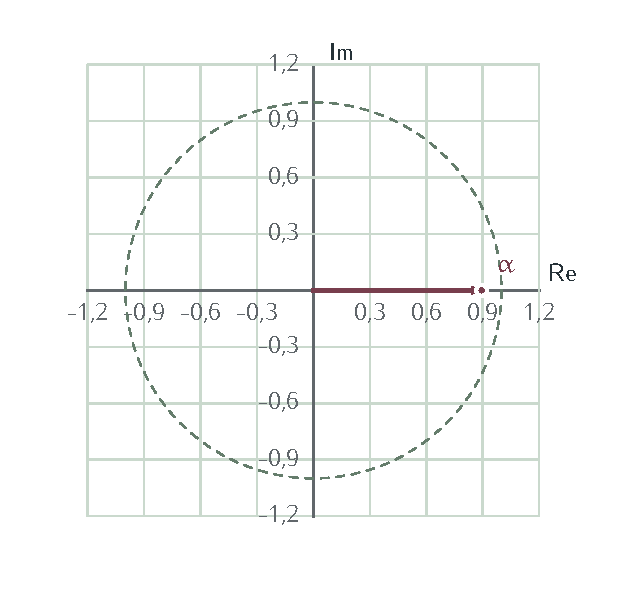
\includegraphics[width=\linewidth,height=63mm,keepaspectratio]{figure/f58bb14f3463ee836.pdf}\par{\sffamily\footnotesize \(\alpha \)\par}\end{minipage}\hfill\begin{minipage}[t]{.485\linewidth}\centering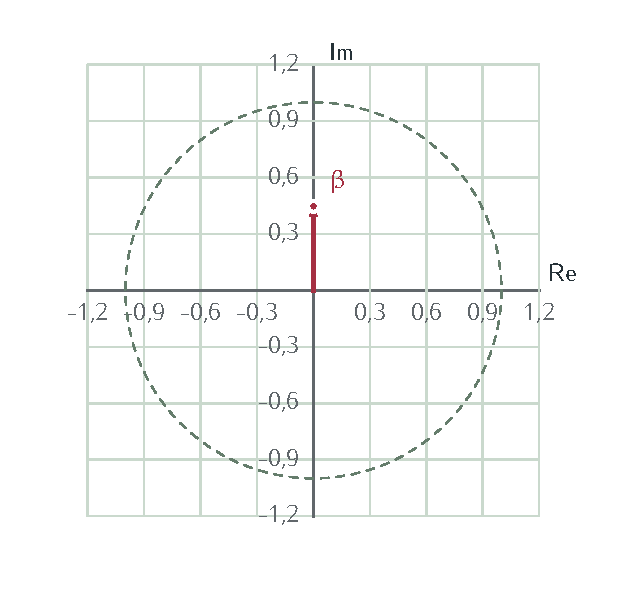
\includegraphics[width=\linewidth,height=63mm,keepaspectratio]{figure/f4551412e5d7210c3.pdf}\par{\sffamily\footnotesize \(\beta \)\par}\end{minipage}\FigureCaption{2.22 \(\cdot\) esempio 1 \(\cdot\) Componenti del ket normalizzato}\end{FigureBlock}
\begin{FigureBlock}\begin{minipage}[t]{.485\linewidth}\centering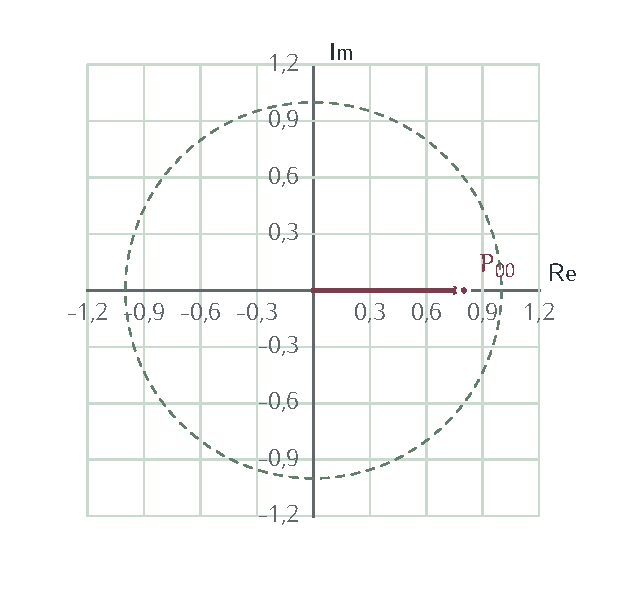
\includegraphics[width=\linewidth,height=63mm,keepaspectratio]{figure/f5fde174e2d30163c.pdf}\par{\sffamily\footnotesize \(P_{00}\)\par}\end{minipage}\hfill\begin{minipage}[t]{.485\linewidth}\centering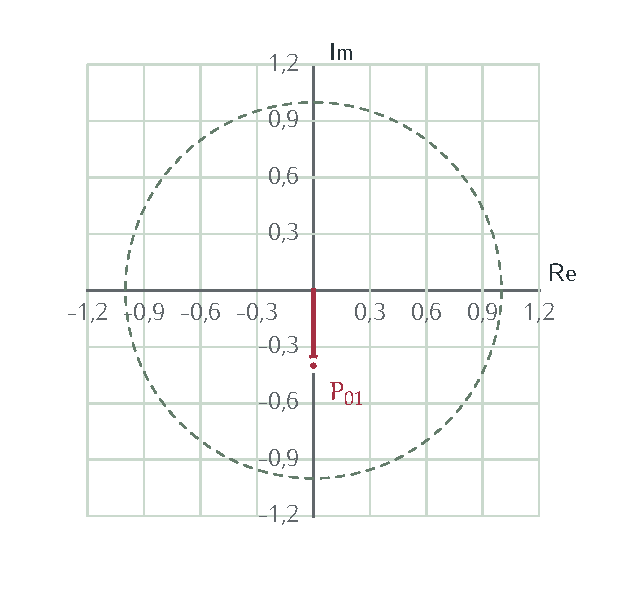
\includegraphics[width=\linewidth,height=63mm,keepaspectratio]{figure/fd9334b98fa559aa9.pdf}\par{\sffamily\footnotesize \(P_{01}\)\par}\end{minipage}\FigureCaption{2.22 \(\cdot\) esempio 1 \(\cdot\) Elementi del prodotto esterno}\end{FigureBlock}
\begin{FigureBlock}\begin{minipage}[t]{.485\linewidth}\centering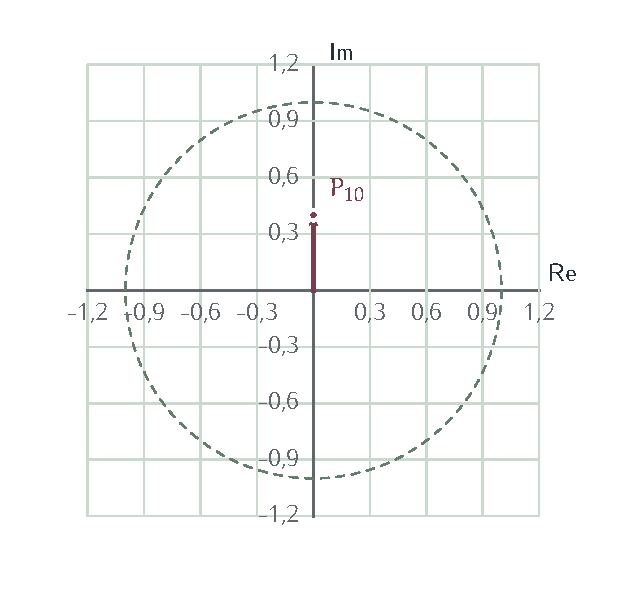
\includegraphics[width=\linewidth,height=63mm,keepaspectratio]{figure/f516cdf6b1e20d426.pdf}\par{\sffamily\footnotesize \(P_{10}\)\par}\end{minipage}\hfill\begin{minipage}[t]{.485\linewidth}\centering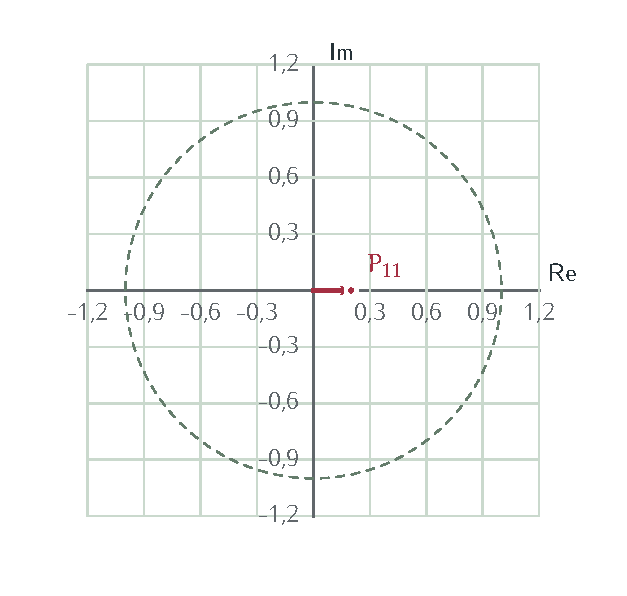
\includegraphics[width=\linewidth,height=63mm,keepaspectratio]{figure/f57952c891c00f46c.pdf}\par{\sffamily\footnotesize \(P_{11}\)\par}\end{minipage}\FigureCaption{2.22 \(\cdot\) esempio 1 \(\cdot\) Elementi del prodotto esterno}\end{FigureBlock}
\begin{FigureBlock}\centering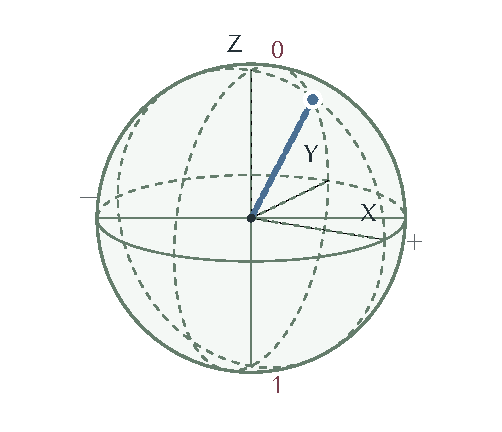
\includegraphics[width=\linewidth,height=94mm,keepaspectratio]{figure/fe3587a4d3c7cb4d0.pdf}\FigureCaption{2.22 \(\cdot\) esempio 1 \(\cdot\) Sfera di Bloch \(\cdot\) stato dell'esempio}\end{FigureBlock}

\phantomsection\label{c2-bra-example-1-step-1}
\BookHeading{01 Normalizzare il dato}

\MathBlock{201600280032002C006900291D40201600B2003D003200B2002B007C0069007C00B2003D0035}{\Vert (2,\allowbreak i)^{T}\Vert ^{2}=2^{2}+|i|^{2}=5}
\MathBlock{03C8003D00280032002C006900291D40002F221A0035003B002003B1003D0032002F221A0035003B002003B2003D0069002F221A0035}{\psi =(2,\allowbreak i)^{T}/\sqrt{5};\allowbreak \ \alpha =2/\sqrt{5};\allowbreak \ \beta =i/\sqrt{5}}

I coefficienti sono riferiti alla base \(|0\rangle =(1{,}0)^{T}\), \(|1\rangle =(0{,}1)^{T}\).\par


\phantomsection\label{c2-bra-example-1-step-2}
\BookHeading{02 Trasporre e coniugare}

\MathBlock{007C03C827E900200063006F006C006F006E006E0061002021D2002027E803C8007C00200072006900670061}{|\psi \rangle \ \text{colonna}\ \Rightarrow \ \langle \psi |\ \text{riga}}
\MathBlock{27E803C8007C003D00280032002C221200690029002F221A0035}{\langle \psi |=(2,\allowbreak - i)/\sqrt{5}}

La trasposizione cambia la forma del vettore; il coniugio cambia i in \(- i\).\par


\phantomsection\label{c2-bra-example-1-step-3}
\BookHeading{03 Moltiplicare riga per colonna}

\MathBlock{27E803C8007C03C827E9003D005B003200B70032002B00282212006900290069005D002F0035003D00280034002B00310029002F0035003D0031}{\langle \psi |\psi \rangle =[2\cdot 2+(- i)i]/5=(4+1)/5=1}
\MathBlock{27E80030007C03C827E9003D0032002F221A0035003B002027E80031007C03C827E9003D0069002F221A0035}{\langle 0|\psi \rangle =2/\sqrt{5};\allowbreak \ \langle 1|\psi \rangle =i/\sqrt{5}}

Il primo prodotto controlla la norma; gli altri due estraggono le coordinate nella base canonica.\par


\phantomsection\label{c2-bra-example-1-step-4}
\BookHeading{04 Moltiplicare colonna per riga}

\MathBlock{0050003D007C03C827E927E803C8007C003D00280031002F00350029005B005B0034002C221200320069005D002C005B00320069002C0031005D005D}{P=|\psi \rangle \langle \psi |=(1/5)\begin{pmatrix}4&- 2i\\2i&1\end{pmatrix}}
\MathBlock{005020802080003D03B103B1002A003B0020005020802081003D03B103B2002A003B0020005020812080003D03B203B1002A003B0020005020812081003D03B203B2002A}{P_{00}=\alpha \alpha {}^{*};\allowbreak \ P_{01}=\alpha \beta {}^{*};\allowbreak \ P_{10}=\beta \alpha {}^{*};\allowbreak \ P_{11}=\beta \beta {}^{*}}

L'ordine invertito produce una matrice 2\(\times\)2, il proiettore sulla direzione \(\psi \).\par


\phantomsection\label{c2-bra-example-1-step-5}
\BookHeading{05 Verificare l'azione del proiettore}

\MathBlock{005003C8003D03C8002827E803C8007C03C827E90029003D03C8}{P\psi =\psi (\langle \psi |\psi \rangle )=\psi }
\MathBlock{005000B2003D007C03C827E9002827E803C8007C03C827E9002927E803C8007C003D0050}{P^{2}=|\psi \rangle (\langle \psi |\psi \rangle )\langle \psi |=P}
\MathBlock{0050007C003027E9003D00280034002C0032006900291D40002F0035}{P|0\rangle =(4{,}2i)^{T}/5}

Applicare il proiettore a \(\psi \) lo conserva; applicarlo a un altro vettore ne estrae la componente lungo \(\psi \).\par


\phantomsection\label{c2-bra-example-1-step-6}
\BookHeading{06 Costruire le coordinate di Bloch}

\MathBlock{03B1002A03B2003D00320069002F0035}{\alpha {}^{*}\beta =2i/5}
\MathBlock{00722093003D003200520065002803B1002A03B20029003D0030003B002000721D67003D00320049006D002803B1002A03B20029003D0034002F0035003B00200072D835DCCF003D007C03B1007C00B22212007C03B2007C00B2003D0033002F0035}{r_{x}=2\operatorname{Re}(\alpha {}^{*}\beta )=0;\allowbreak \ r_{y}=2\operatorname{Im}(\alpha {}^{*}\beta )=4/5;\allowbreak \ r_{z}=|\alpha |^{2}- |\beta |^{2}=3/5}
\MathBlock{0072003D00280030003B00200030002C0038003B00200030002C00360029003B002020160072201600B2003D00280034002F0035002900B2002B00280033002F0035002900B2003D0031}{r=(0;\allowbreak \ 0{,}8;\allowbreak \ 0{,}6);\allowbreak \ \Vert r\Vert ^{2}=(4/5)^{2}+(3/5)^{2}=1}

La sfera è ottenuta dalle ampiezze e identifica vettori che differiscono per una fase globale. Le sue coordinate sono adimensionali.\par


\BookHeading{Interpretazione}

Il prodotto interno restituisce lo scalare 1; il prodotto esterno restituisce il proiettore \(P\). La figura di Bloch rappresenta la stessa direzione pura \(r=(0\); 0,8; 0,6).\par


\Needspace{.36\textheight}\phantomsection\label{c2-bra-example-2}
{\sffamily\small\color{Accent} ESEMPIO SVOLTO 2\par}
\BookHeading{Prodotto esterno sullo stato equatoriale}
Dati \(\psi \) \(\text{grezzo}=(1,\allowbreak i)^{T}\) e base computazionale \(|0\rangle =(1{,}0)^{T}\), \(|1\rangle =(0{,}1)^{T}\).\par


\BookHeading{Geometria e configurazione dell'esempio}
\begin{FigureBlock}\begin{minipage}[t]{.485\linewidth}\centering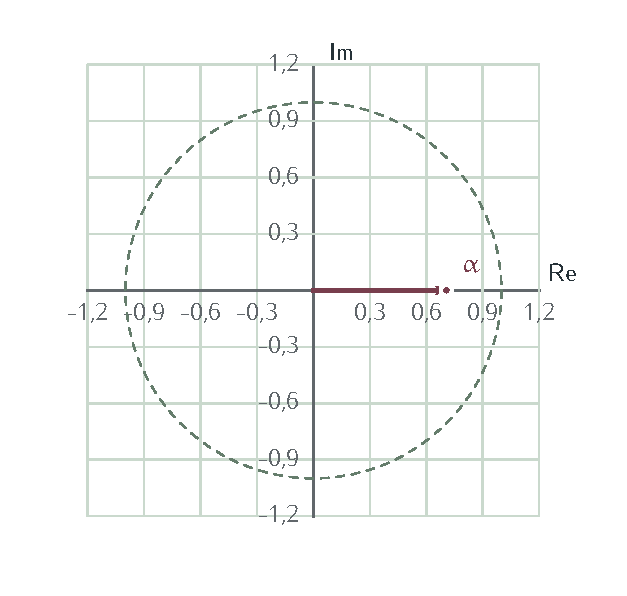
\includegraphics[width=\linewidth,height=63mm,keepaspectratio]{figure/fd88de13169590779.pdf}\par{\sffamily\footnotesize \(\alpha \)\par}\end{minipage}\hfill\begin{minipage}[t]{.485\linewidth}\centering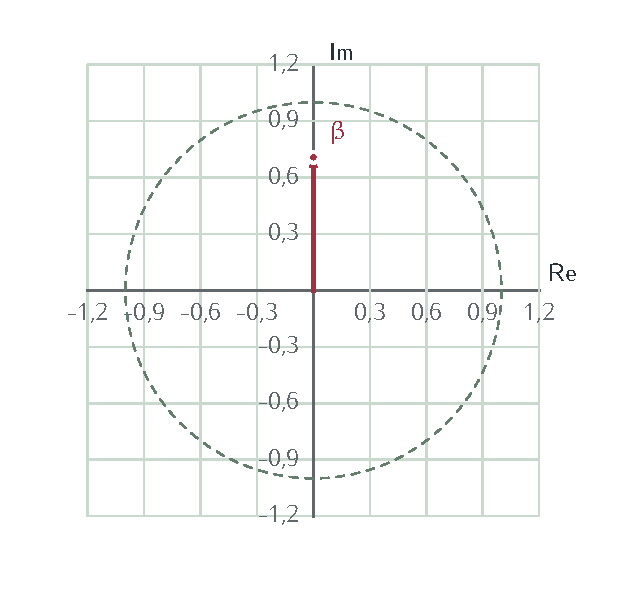
\includegraphics[width=\linewidth,height=63mm,keepaspectratio]{figure/fb7576a3f3d8ba6ee.pdf}\par{\sffamily\footnotesize \(\beta \)\par}\end{minipage}\FigureCaption{2.22 \(\cdot\) esempio 2 \(\cdot\) Componenti del ket normalizzato}\end{FigureBlock}
\begin{FigureBlock}\begin{minipage}[t]{.485\linewidth}\centering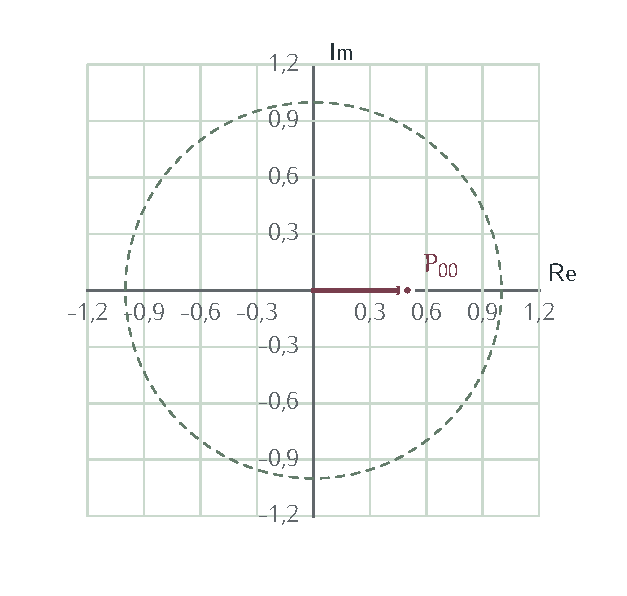
\includegraphics[width=\linewidth,height=63mm,keepaspectratio]{figure/f17029c4b82ad5738.pdf}\par{\sffamily\footnotesize \(P_{00}\)\par}\end{minipage}\hfill\begin{minipage}[t]{.485\linewidth}\centering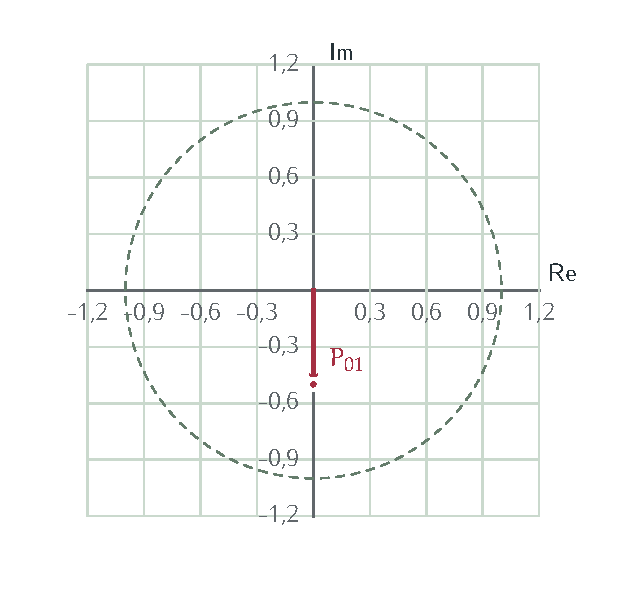
\includegraphics[width=\linewidth,height=63mm,keepaspectratio]{figure/fc7ef84953d7b9157.pdf}\par{\sffamily\footnotesize \(P_{01}\)\par}\end{minipage}\FigureCaption{2.22 \(\cdot\) esempio 2 \(\cdot\) Elementi del prodotto esterno}\end{FigureBlock}
\begin{FigureBlock}\begin{minipage}[t]{.485\linewidth}\centering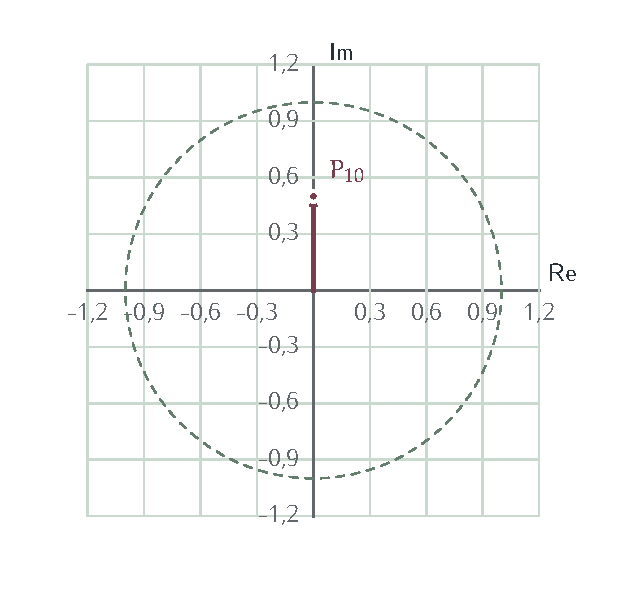
\includegraphics[width=\linewidth,height=63mm,keepaspectratio]{figure/f3484fb668eea4f2d.pdf}\par{\sffamily\footnotesize \(P_{10}\)\par}\end{minipage}\hfill\begin{minipage}[t]{.485\linewidth}\centering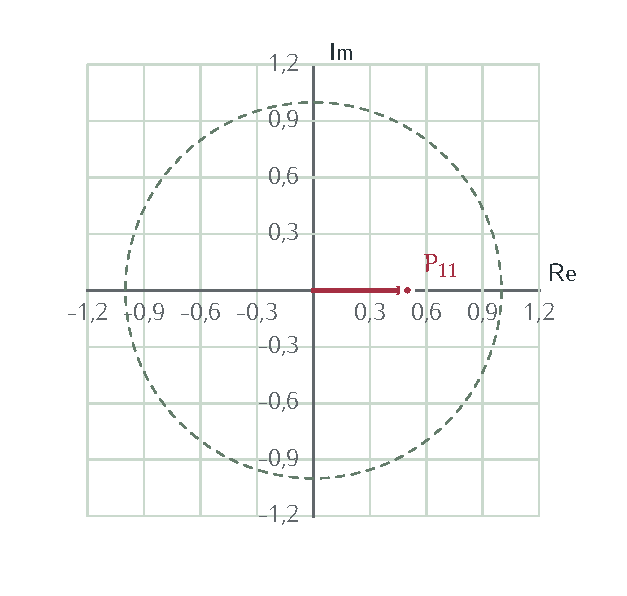
\includegraphics[width=\linewidth,height=63mm,keepaspectratio]{figure/f1d3e742f7ea957e8.pdf}\par{\sffamily\footnotesize \(P_{11}\)\par}\end{minipage}\FigureCaption{2.22 \(\cdot\) esempio 2 \(\cdot\) Elementi del prodotto esterno}\end{FigureBlock}
\begin{FigureBlock}\centering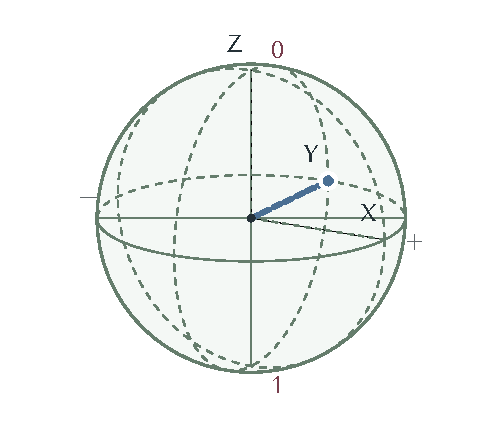
\includegraphics[width=\linewidth,height=94mm,keepaspectratio]{figure/fae21600cc1d0968b.pdf}\FigureCaption{2.22 \(\cdot\) esempio 2 \(\cdot\) Sfera di Bloch \(\cdot\) stato dell'esempio}\end{FigureBlock}

\phantomsection\label{c2-bra-example-2-step-1}
\BookHeading{01 Normalizzare il dato}

\MathBlock{201600280031002C006900291D40201600B2003D003100B2002B007C0069007C00B2003D0032}{\Vert (1,\allowbreak i)^{T}\Vert ^{2}=1^{2}+|i|^{2}=2}
\MathBlock{03C8003D00280031002C006900291D40002F221A0032003B002003B1003D0031002F221A0032003B002003B2003D0069002F221A0032}{\psi =(1,\allowbreak i)^{T}/\sqrt{2};\allowbreak \ \alpha =1/\sqrt{2};\allowbreak \ \beta =i/\sqrt{2}}

I coefficienti sono riferiti alla base \(|0\rangle =(1{,}0)^{T}\), \(|1\rangle =(0{,}1)^{T}\).\par


\phantomsection\label{c2-bra-example-2-step-2}
\BookHeading{02 Trasporre e coniugare}

\MathBlock{007C03C827E900200063006F006C006F006E006E0061002021D2002027E803C8007C00200072006900670061}{|\psi \rangle \ \text{colonna}\ \Rightarrow \ \langle \psi |\ \text{riga}}
\MathBlock{27E803C8007C003D00280031002C221200690029002F221A0032}{\langle \psi |=(1,\allowbreak - i)/\sqrt{2}}

La trasposizione cambia la forma del vettore; il coniugio cambia i in \(- i\).\par


\phantomsection\label{c2-bra-example-2-step-3}
\BookHeading{03 Moltiplicare riga per colonna}

\MathBlock{27E803C8007C03C827E9003D005B003100B70031002B00282212006900290069005D002F0032003D00280031002B00310029002F0032003D0031}{\langle \psi |\psi \rangle =[1\cdot 1+(- i)i]/2=(1+1)/2=1}
\MathBlock{27E80030007C03C827E9003D0031002F221A0032003B002027E80031007C03C827E9003D0069002F221A0032}{\langle 0|\psi \rangle =1/\sqrt{2};\allowbreak \ \langle 1|\psi \rangle =i/\sqrt{2}}

Il primo prodotto controlla la norma; gli altri due estraggono le coordinate nella base canonica.\par


\phantomsection\label{c2-bra-example-2-step-4}
\BookHeading{04 Moltiplicare colonna per riga}

\MathBlock{0050003D007C03C827E927E803C8007C003D00280031002F00320029005B005B0031002C221200310069005D002C005B00310069002C0031005D005D}{P=|\psi \rangle \langle \psi |=(1/2)\begin{pmatrix}1&- 1i\\1i&1\end{pmatrix}}
\MathBlock{005020802080003D03B103B1002A003B0020005020802081003D03B103B2002A003B0020005020812080003D03B203B1002A003B0020005020812081003D03B203B2002A}{P_{00}=\alpha \alpha {}^{*};\allowbreak \ P_{01}=\alpha \beta {}^{*};\allowbreak \ P_{10}=\beta \alpha {}^{*};\allowbreak \ P_{11}=\beta \beta {}^{*}}

L'ordine invertito produce una matrice 2\(\times\)2, il proiettore sulla direzione \(\psi \).\par


\phantomsection\label{c2-bra-example-2-step-5}
\BookHeading{05 Verificare l'azione del proiettore}

\MathBlock{005003C8003D03C8002827E803C8007C03C827E90029003D03C8}{P\psi =\psi (\langle \psi |\psi \rangle )=\psi }
\MathBlock{005000B2003D007C03C827E9002827E803C8007C03C827E9002927E803C8007C003D0050}{P^{2}=|\psi \rangle (\langle \psi |\psi \rangle )\langle \psi |=P}
\MathBlock{0050007C003027E9003D00280031002C0031006900291D40002F0032}{P|0\rangle =(1{,}1i)^{T}/2}

Applicare il proiettore a \(\psi \) lo conserva; applicarlo a un altro vettore ne estrae la componente lungo \(\psi \).\par


\phantomsection\label{c2-bra-example-2-step-6}
\BookHeading{06 Costruire le coordinate di Bloch}

\MathBlock{03B1002A03B2003D00310069002F0032}{\alpha {}^{*}\beta =1i/2}
\MathBlock{00722093003D003200520065002803B1002A03B20029003D0030003B002000721D67003D00320049006D002803B1002A03B20029003D0032002F0032003B00200072D835DCCF003D007C03B1007C00B22212007C03B2007C00B2003D0030002F0032}{r_{x}=2\operatorname{Re}(\alpha {}^{*}\beta )=0;\allowbreak \ r_{y}=2\operatorname{Im}(\alpha {}^{*}\beta )=2/2;\allowbreak \ r_{z}=|\alpha |^{2}- |\beta |^{2}=0/2}
\MathBlock{0072003D00280030003B00200031003B002000300029003B002020160072201600B2003D00280032002F0032002900B2002B00280030002F0032002900B2003D0031}{r=(0;\allowbreak \ 1;\allowbreak \ 0);\allowbreak \ \Vert r\Vert ^{2}=(2/2)^{2}+(0/2)^{2}=1}

La sfera è ottenuta dalle ampiezze e identifica vettori che differiscono per una fase globale. Le sue coordinate sono adimensionali.\par


\BookHeading{Interpretazione}

Il prodotto interno restituisce lo scalare 1; il prodotto esterno restituisce il proiettore \(P\). La figura di Bloch rappresenta la stessa direzione pura \(r=(0\); 1; 0).\par


\Needspace{7\baselineskip}
\BookHeading{Il passaggio successivo}
Il bra calcola coefficienti rispetto a una direzione. Nelle basi \(X\) e \(Z\) useremo questi coefficienti per rendere visibile il ruolo della fase relativa.\par


\Needspace{.43\textheight}
\section{Fase relativa e interferenza}
\phantomsection\label{c2-fase}

{\sffamily\small\color{Ink!70} Riferimento alle slide: p. 319.\par}

{\sffamily\small\color{Ink!70} Laboratorio locale: \nolinkurl{index.html#capitolo-2/fase}\par}

\BookHeading{Definizioni e costruzione}
Una fase relativa modifica il modo in cui le ampiezze si sommano in un'altra base. Confrontiamo la misura \(Z\) con la ricombinazione nella base \(X\).\par

Dichiariamo le basi che useremo: la base \(Z\) è \(\{|0\rangle ,\allowbreak |1\rangle \}\); la base \(X\) è \(\{|+\rangle ,\allowbreak |- \rangle \}\), con \(|+\rangle =(|0\rangle +|1\rangle )/\sqrt{2}\) e \(|- \rangle =(|0\rangle - |1\rangle )/\sqrt{2}\). La matrice \(H=(1/\sqrt{2})\)\(\begin{pmatrix}1&1\\1&- 1\end{pmatrix}\), detta Hadamard, raccoglie questi ultimi vettori come colonne; \(H{}^{\dagger} =H\) e \(H{}^{\dagger} H=I\). Le coordinate nella base \(X\) sono quindi \(H{}^{\dagger} \psi =H\psi \).\par

Le matrici di Pauli sono \(X=\)\(\begin{pmatrix}0&1\\1&0\end{pmatrix}\), \(Y=\)\(\begin{pmatrix}0&- i\\i&0\end{pmatrix}\), \(Z=\)\(\begin{pmatrix}1&0\\0&- 1\end{pmatrix}\). Sono hermitiane e hanno autovalori +1 e \(- 1\). Le basi proprie sono rispettivamente \(\{|+\rangle ,\allowbreak |- \rangle \}\), \(\{(1,\allowbreak i)/\sqrt{2},\allowbreak (1,\allowbreak - i)/\sqrt{2}\}\) e \(\{|0\rangle ,\allowbreak |1\rangle \}\). Per esempio \(X(1,\allowbreak \pm 1)^{T}=\pm (1,\allowbreak \pm 1)^{T}\) e \(Z(1{,}0)^{T}=(1{,}0)^{T}\). Le etichette delle basi vanno distinte dai valori \(\pm 1\) degli esiti.\par

Nella famiglia \(\psi \varphi =(1,\allowbreak e^{i\varphi })^{T}/\sqrt{2}\), i moduli delle componenti \(Z\) restano uguali al variare di \(\varphi \). Nella base \(X\) il prodotto interno somma o sottrae le componenti: \(a\pm =(1\pm e^{i\varphi })/2\). Sviluppandone il modulo quadro si ottiene \(p\pm =(1\pm \cos \varphi )/2\). I casi \(90{}^{\circ} \), \(180{}^{\circ} \) e \(0{}^{\circ} \) mostrano rispettivamente pesi uguali, cancellazione della somma e cancellazione della differenza.\par

Moltiplicando entrambe le componenti per \(e^{i\gamma }\), ogni ampiezza di misura riceve lo stesso fattore di modulo uno e tutte le probabilità restano invariate. Nel disegno di Bloch questa fase globale è già eliminata, mentre la fase relativa determina la posizione \(r=(\cos \varphi ,\allowbreak \sin \varphi ,\allowbreak 0)\) sull'equatore.\par


\MathBlock{007C03C803C627E9003D0028007C003027E9002B0065005E0028006903C60029007C003127E90029002F221A0032003B002027E800B1007C03C803C627E9003D0028003100B10065005E0028006903C600290029002F0032002E}{|\psi \varphi \rangle =(|0\rangle +e^{i\varphi }|1\rangle )/\sqrt{2};\allowbreak \ \langle \pm |\psi \varphi \rangle =(1\pm e^{i\varphi })/2.}

\BookHeading{Come leggere le figure}
Due componenti complesse; sulla sfera di Bloch \(r=(\cos \varphi ,\allowbreak \sin \varphi ,\allowbreak 0)\).\par


\Needspace{.36\textheight}\phantomsection\label{c2-fase-example-1}
{\sffamily\small\color{Accent} ESEMPIO SVOLTO 1\par}
\BookHeading{Fase relativa \(90{}^{\circ} \)}
Dati \(\varphi =90{}^{\circ} \) e \(\psi \varphi =(|0\rangle +e^{i\varphi }|1\rangle )/\sqrt{2}\); confrontiamo le basi \(Z\) e \(X\).\par


\BookHeading{Geometria e configurazione dell'esempio}
\begin{FigureBlock}\begin{minipage}[t]{.485\linewidth}\centering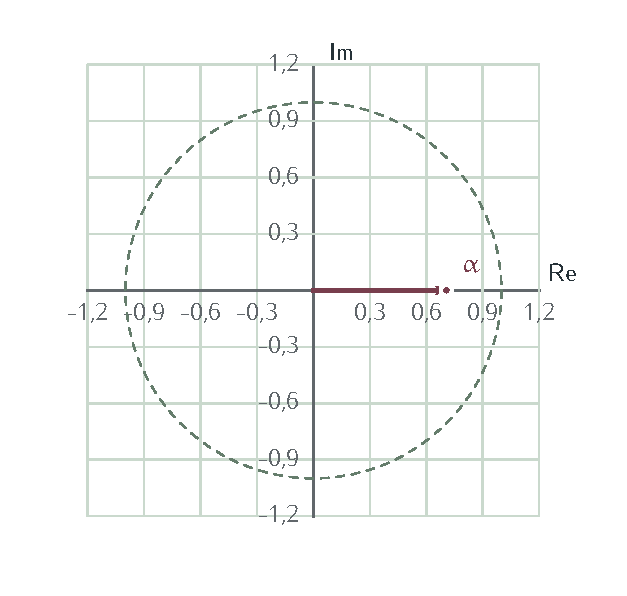
\includegraphics[width=\linewidth,height=63mm,keepaspectratio]{figure/fcdc350f71d8d0cb9.pdf}\par{\sffamily\footnotesize \(\alpha \)\par}\end{minipage}\hfill\begin{minipage}[t]{.485\linewidth}\centering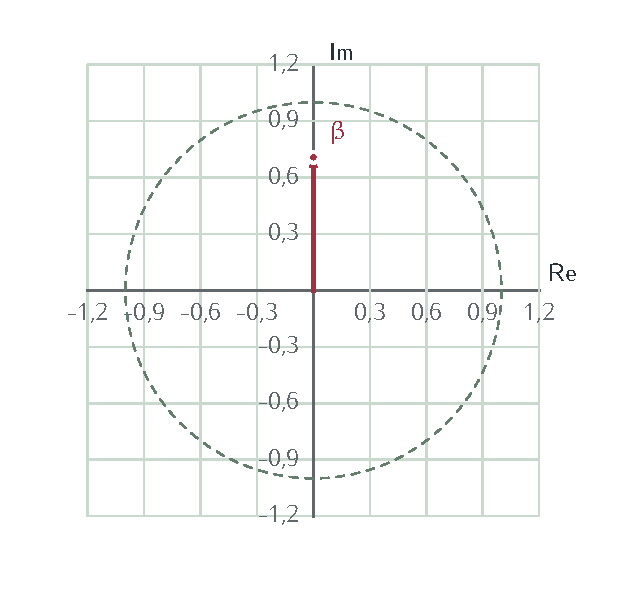
\includegraphics[width=\linewidth,height=63mm,keepaspectratio]{figure/fda7822cd0f6212c4.pdf}\par{\sffamily\footnotesize \(\beta \)\par}\end{minipage}\FigureCaption{2.23 \(\cdot\) esempio 1 \(\cdot\) Componenti dello stato con fase relativa}\end{FigureBlock}
\begin{FigureBlock}\centering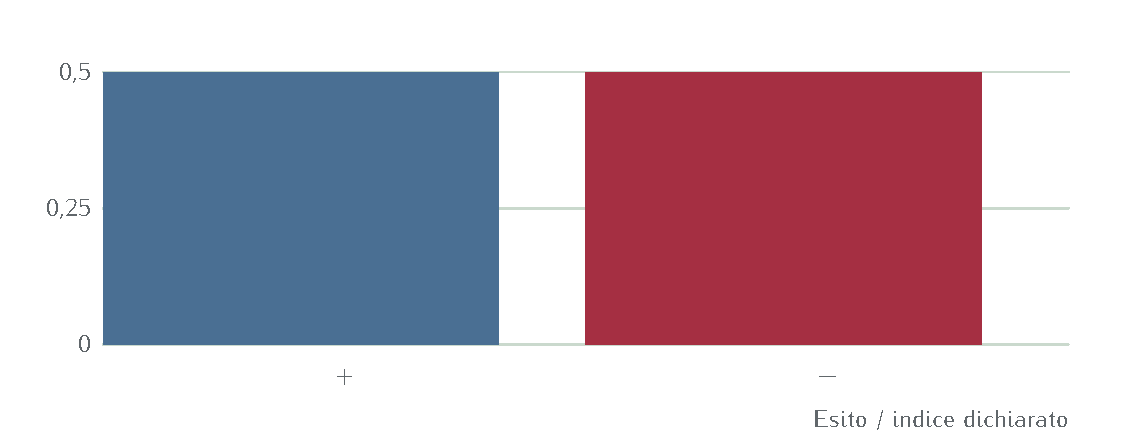
\includegraphics[width=\linewidth,height=94mm,keepaspectratio]{figure/f33cfc2b3241b49b9.pdf}\FigureCaption{2.23 \(\cdot\) esempio 1 \(\cdot\) Probabilità dopo la ricombinazione in \(X\)}\end{FigureBlock}
\begin{FigureBlock}\centering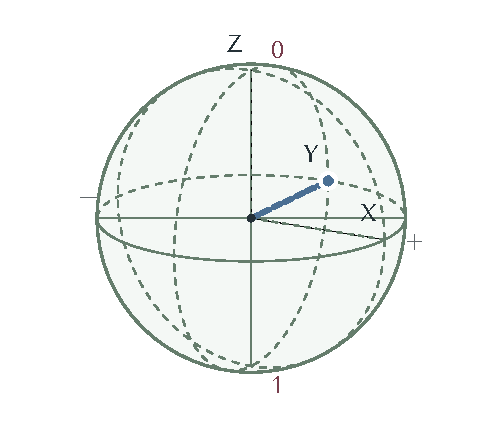
\includegraphics[width=\linewidth,height=94mm,keepaspectratio]{figure/fae21600cc1d0968b.pdf}\FigureCaption{2.23 \(\cdot\) esempio 1 \(\cdot\) Sfera di Bloch \(\cdot\) stato dell'esempio}\end{FigureBlock}

\phantomsection\label{c2-fase-example-1-step-1}
\BookHeading{01 Dichiarare le due basi}

\MathBlock{00420061007300650020005A003A0020007C003027E9003D00280031002C003000291D40002C0020007C003127E9003D00280030002C003100291D40}{\text{Base}\ Z:\ |0\rangle =(1{,}0)^{T},\allowbreak \ |1\rangle =(0{,}1)^{T}}
\MathBlock{004200610073006500200058003A0020007C002B27E9003D00280031002C003100291D40002F221A0032002C0020007C221227E9003D00280031002C2212003100291D40002F221A0032}{\text{Base}\ X:\ |+\rangle =(1{,}1)^{T}/\sqrt{2},\allowbreak \ |- \rangle =(1,\allowbreak - 1)^{T}/\sqrt{2}}

I prodotti interni con questi vettori danno i coefficienti nelle due basi.\par


\phantomsection\label{c2-fase-example-1-step-2}
\BookHeading{02 Inserire la fase relativa}

\MathBlock{03C6003D0039003000B0003B00200065005E0028006903C60029003D0069}{\varphi =90{}^{\circ} ;\allowbreak \ e^{i\varphi }=i}
\MathBlock{03C803C6003D00280031002C006900291D40002F221A0032003B0020007C03B1007C00B2003D007C03B2007C00B2003D0031002F0032}{\psi \varphi =(1,\allowbreak i)^{T}/\sqrt{2};\allowbreak \ |\alpha |^{2}=|\beta |^{2}=1/2}

Il primo coefficiente è reale positivo; il secondo porta la fase relativa dichiarata.\par


\phantomsection\label{c2-fase-example-1-step-3}
\BookHeading{03 Calcolare i coefficienti nella base \(X\)}

\MathBlock{0061208A003D00280031002B0028006900290029002F0032003D0030002C00350020002B00200030002C00350069}{a_{+}=(1+(i))/2=0{,}5\ +\ 0{,}5i}
\MathBlock{0061208B003D0028003122120028006900290029002F0032003D0030002C00350020221200200030002C00350069}{a_{-}=(1- (i))/2=0{,}5\ - \ 0{,}5i}

La base \(X\) combina le due componenti mediante somma e differenza.\par


\phantomsection\label{c2-fase-example-1-step-4}
\BookHeading{04 Calcolare i pesi della ricombinazione}

\MathBlock{0070002B003D002800280030002C0035002900B20020002B002000280030002C0035002900B20029003D0030002C0035}{p+=((0{,}5)^{2}\ +\ (0{,}5)^{2})=0{,}5}
\MathBlock{00702212003D002800280030002C0035002900B20020002B00200028002D0030002C0035002900B20029003D0030002C0035}{p- =((0{,}5)^{2}\ +\ (-0{,}5)^{2})=0{,}5}

Le probabilità \(Z\) restano (1/2,1/2); quelle \(X\) dipendono dalla fase.\par


\phantomsection\label{c2-fase-example-1-step-5}
\BookHeading{05 Posizionare lo stato sull'equatore}

\MathBlock{0072003D00280063006F0073002003C6002C00730069006E002003C6002C00300029003D00280030003B00200031003B002000300029}{r=(\cos \ \varphi ,\allowbreak \sin \ \varphi ,\allowbreak 0)=(0;\allowbreak \ 1;\allowbreak \ 0)}
\MathBlock{0070208A003D00280031002B0063006F0073002003C60029002F0032003B00200070208B003D0028003122120063006F0073002003C60029002F0032}{p_{+}=(1+\cos \ \varphi )/2;\allowbreak \ p_{-}=(1- \cos \ \varphi )/2}

Il valore della coordinata x coincide con la differenza fra i due pesi \(X\).\par


\phantomsection\label{c2-fase-example-1-step-6}
\BookHeading{06 Verificare l'invarianza globale}

\MathBlock{03C82032003D006903C8003B002027E80075007C03C8203227E9003D006927E80075007C03C827E9}{\psi {}^{\prime} =i\psi ;\allowbreak \ \langle u|\psi {}^{\prime} \rangle =i\langle u|\psi \rangle }
\MathBlock{007C27E80075007C03C8203227E9007C00B2003D007C0069007C00B2007C27E80075007C03C827E9007C00B2003D007C27E80075007C03C827E9007C00B2}{|\langle u|\psi {}^{\prime} \rangle |^{2}=|i|^{2}|\langle u|\psi \rangle |^{2}=|\langle u|\psi \rangle |^{2}}

La fase comune moltiplica tutte le ampiezze di misura per un fattore di modulo uno.\par


\BookHeading{Interpretazione}

Le due somme complesse hanno moduli uguali: gli esiti \(X\) sono equiprobabili.\par


\Needspace{.36\textheight}\phantomsection\label{c2-fase-example-2}
{\sffamily\small\color{Accent} ESEMPIO SVOLTO 2\par}
\BookHeading{Fase relativa \(180{}^{\circ} \)}
Dati \(\varphi =180{}^{\circ} \) e \(\psi \varphi =(|0\rangle +e^{i\varphi }|1\rangle )/\sqrt{2}\); confrontiamo le basi \(Z\) e \(X\).\par


\BookHeading{Geometria e configurazione dell'esempio}
\begin{FigureBlock}\begin{minipage}[t]{.485\linewidth}\centering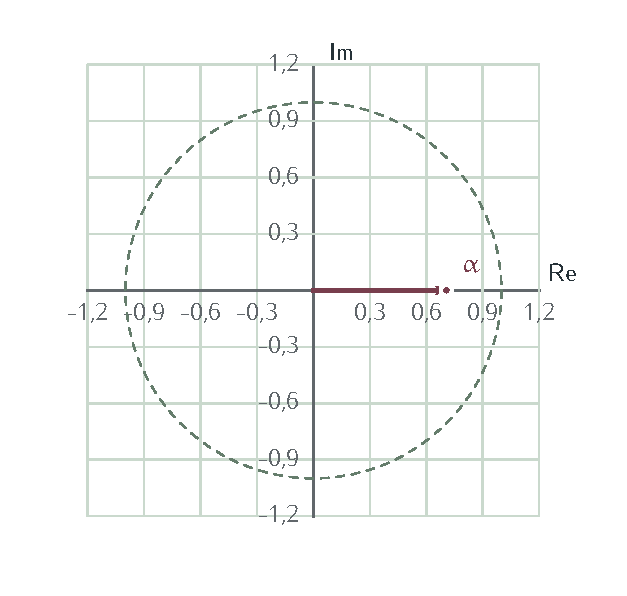
\includegraphics[width=\linewidth,height=63mm,keepaspectratio]{figure/fd88de13169590779.pdf}\par{\sffamily\footnotesize \(\alpha \)\par}\end{minipage}\hfill\begin{minipage}[t]{.485\linewidth}\centering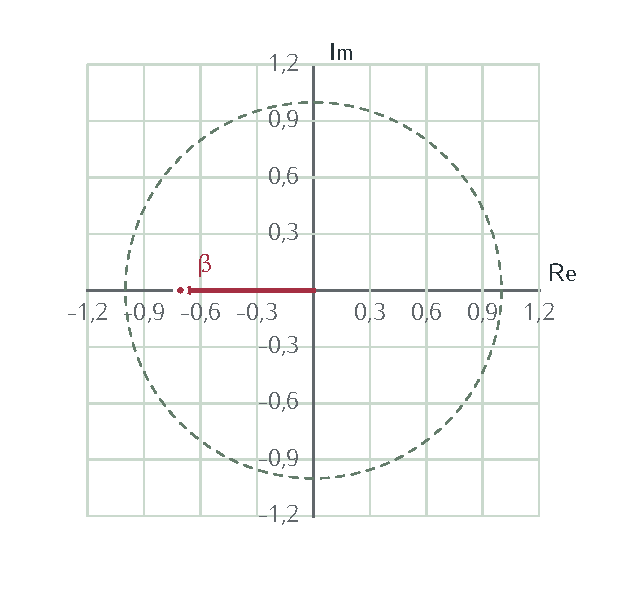
\includegraphics[width=\linewidth,height=63mm,keepaspectratio]{figure/f66a2f2a7f65a8bfe.pdf}\par{\sffamily\footnotesize \(\beta \)\par}\end{minipage}\FigureCaption{2.23 \(\cdot\) esempio 2 \(\cdot\) Componenti dello stato con fase relativa}\end{FigureBlock}
\begin{FigureBlock}\centering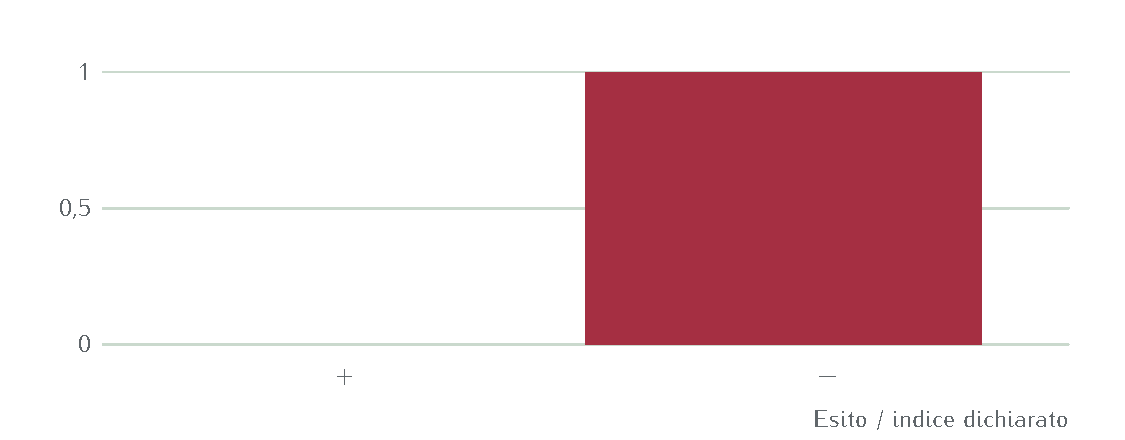
\includegraphics[width=\linewidth,height=94mm,keepaspectratio]{figure/f9499f277bc42a0c0.pdf}\FigureCaption{2.23 \(\cdot\) esempio 2 \(\cdot\) Probabilità dopo la ricombinazione in \(X\)}\end{FigureBlock}
\begin{FigureBlock}\centering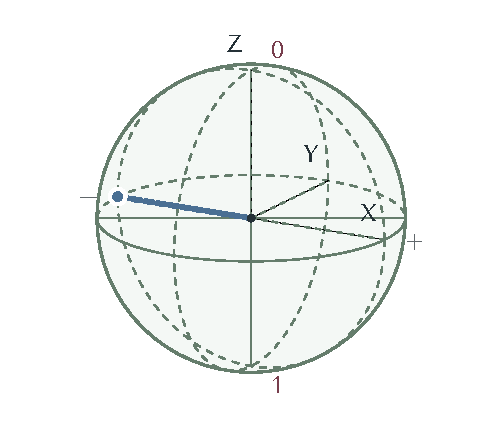
\includegraphics[width=\linewidth,height=94mm,keepaspectratio]{figure/f6124c90aa2e7e801.pdf}\FigureCaption{2.23 \(\cdot\) esempio 2 \(\cdot\) Sfera di Bloch \(\cdot\) stato dell'esempio}\end{FigureBlock}

\phantomsection\label{c2-fase-example-2-step-1}
\BookHeading{01 Dichiarare le due basi}

\MathBlock{00420061007300650020005A003A0020007C003027E9003D00280031002C003000291D40002C0020007C003127E9003D00280030002C003100291D40}{\text{Base}\ Z:\ |0\rangle =(1{,}0)^{T},\allowbreak \ |1\rangle =(0{,}1)^{T}}
\MathBlock{004200610073006500200058003A0020007C002B27E9003D00280031002C003100291D40002F221A0032002C0020007C221227E9003D00280031002C2212003100291D40002F221A0032}{\text{Base}\ X:\ |+\rangle =(1{,}1)^{T}/\sqrt{2},\allowbreak \ |- \rangle =(1,\allowbreak - 1)^{T}/\sqrt{2}}

I prodotti interni con questi vettori danno i coefficienti nelle due basi.\par


\phantomsection\label{c2-fase-example-2-step-2}
\BookHeading{02 Inserire la fase relativa}

\MathBlock{03C6003D00310038003000B0003B00200065005E0028006903C60029003D002D0031}{\varphi =180{}^{\circ} ;\allowbreak \ e^{i\varphi }=-1}
\MathBlock{03C803C6003D00280031002C002D003100291D40002F221A0032003B0020007C03B1007C00B2003D007C03B2007C00B2003D0031002F0032}{\psi \varphi =(1,\allowbreak -1)^{T}/\sqrt{2};\allowbreak \ |\alpha |^{2}=|\beta |^{2}=1/2}

Il primo coefficiente è reale positivo; il secondo porta la fase relativa dichiarata.\par


\phantomsection\label{c2-fase-example-2-step-3}
\BookHeading{03 Calcolare i coefficienti nella base \(X\)}

\MathBlock{0061208A003D00280031002B0028002D003100290029002F0032003D0030}{a_{+}=(1+(-1))/2=0}
\MathBlock{0061208B003D0028003122120028002D003100290029002F0032003D0031}{a_{-}=(1- (-1))/2=1}

La base \(X\) combina le due componenti mediante somma e differenza.\par


\phantomsection\label{c2-fase-example-2-step-4}
\BookHeading{04 Calcolare i pesi della ricombinazione}

\MathBlock{0070002B003D002800280030002900B20020002B002000280030002900B20029003D0030}{p+=((0)^{2}\ +\ (0)^{2})=0}
\MathBlock{00702212003D002800280031002900B20020002B002000280030002900B20029003D0031}{p- =((1)^{2}\ +\ (0)^{2})=1}

Le probabilità \(Z\) restano (1/2,1/2); quelle \(X\) dipendono dalla fase.\par


\phantomsection\label{c2-fase-example-2-step-5}
\BookHeading{05 Posizionare lo stato sull'equatore}

\MathBlock{0072003D00280063006F0073002003C6002C00730069006E002003C6002C00300029003D0028002D0031003B00200030003B002000300029}{r=(\cos \ \varphi ,\allowbreak \sin \ \varphi ,\allowbreak 0)=(-1;\allowbreak \ 0;\allowbreak \ 0)}
\MathBlock{0070208A003D00280031002B0063006F0073002003C60029002F0032003B00200070208B003D0028003122120063006F0073002003C60029002F0032}{p_{+}=(1+\cos \ \varphi )/2;\allowbreak \ p_{-}=(1- \cos \ \varphi )/2}

Il valore della coordinata x coincide con la differenza fra i due pesi \(X\).\par


\phantomsection\label{c2-fase-example-2-step-6}
\BookHeading{06 Verificare l'invarianza globale}

\MathBlock{03C82032003D006903C8003B002027E80075007C03C8203227E9003D006927E80075007C03C827E9}{\psi {}^{\prime} =i\psi ;\allowbreak \ \langle u|\psi {}^{\prime} \rangle =i\langle u|\psi \rangle }
\MathBlock{007C27E80075007C03C8203227E9007C00B2003D007C0069007C00B2007C27E80075007C03C827E9007C00B2003D007C27E80075007C03C827E9007C00B2}{|\langle u|\psi {}^{\prime} \rangle |^{2}=|i|^{2}|\langle u|\psi \rangle |^{2}=|\langle u|\psi \rangle |^{2}}

La fase comune moltiplica tutte le ampiezze di misura per un fattore di modulo uno.\par


\BookHeading{Interpretazione}

La somma si cancella e la differenza vale due: \(X\) dà sempre \(- 1\), pur conservando probabilità \(Z\) uniformi.\par


\Needspace{.36\textheight}\phantomsection\label{c2-fase-example-3}
{\sffamily\small\color{Accent} ESEMPIO SVOLTO 3\par}
\BookHeading{Fase relativa \(0{}^{\circ} \)}
Dati \(\varphi =0{}^{\circ} \) e \(\psi \varphi =(|0\rangle +e^{i\varphi }|1\rangle )/\sqrt{2}\); confrontiamo le basi \(Z\) e \(X\).\par


\BookHeading{Geometria e configurazione dell'esempio}
\begin{FigureBlock}\begin{minipage}[t]{.485\linewidth}\centering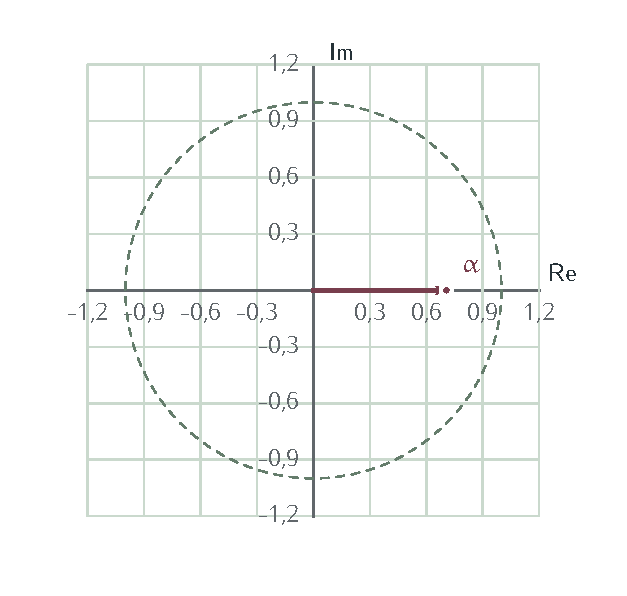
\includegraphics[width=\linewidth,height=63mm,keepaspectratio]{figure/fc046638091b149df.pdf}\par{\sffamily\footnotesize \(\alpha \)\par}\end{minipage}\hfill\begin{minipage}[t]{.485\linewidth}\centering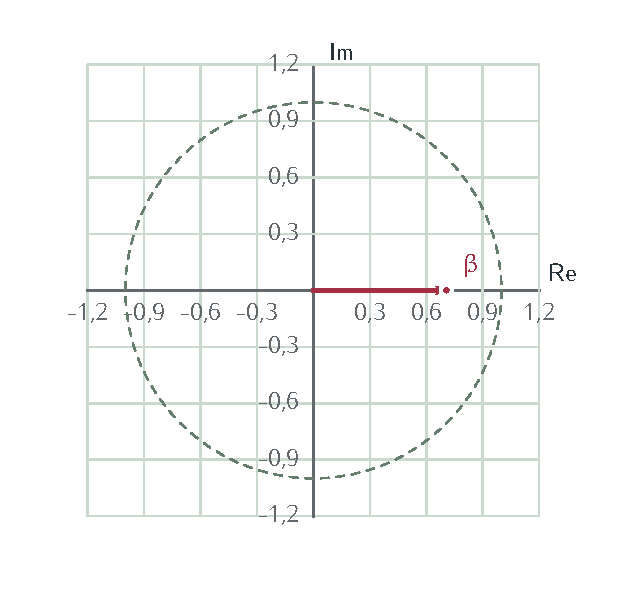
\includegraphics[width=\linewidth,height=63mm,keepaspectratio]{figure/f2225dee882386fff.pdf}\par{\sffamily\footnotesize \(\beta \)\par}\end{minipage}\FigureCaption{2.23 \(\cdot\) esempio 3 \(\cdot\) Componenti dello stato con fase relativa}\end{FigureBlock}
\begin{FigureBlock}\centering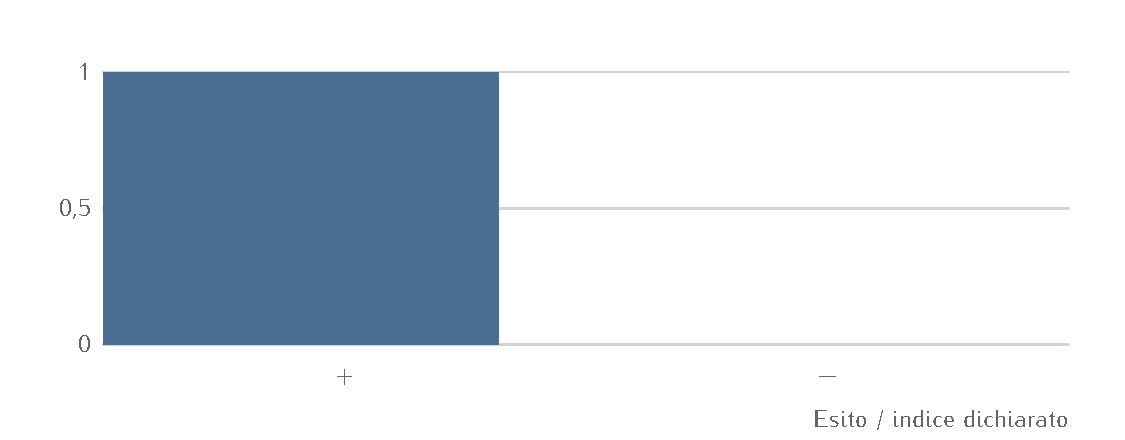
\includegraphics[width=\linewidth,height=94mm,keepaspectratio]{figure/ff18989675216325d.pdf}\FigureCaption{2.23 \(\cdot\) esempio 3 \(\cdot\) Probabilità dopo la ricombinazione in \(X\)}\end{FigureBlock}
\begin{FigureBlock}\centering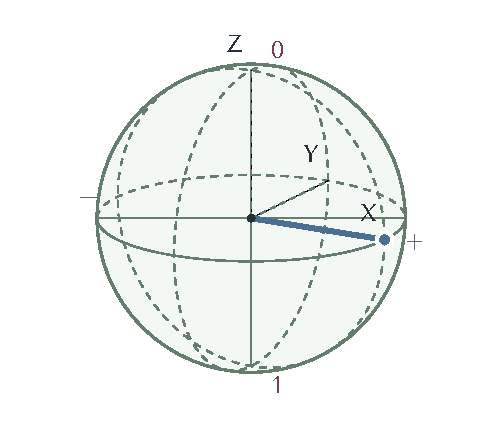
\includegraphics[width=\linewidth,height=94mm,keepaspectratio]{figure/f82d7f056487f5570.pdf}\FigureCaption{2.23 \(\cdot\) esempio 3 \(\cdot\) Sfera di Bloch \(\cdot\) stato dell'esempio}\end{FigureBlock}

\phantomsection\label{c2-fase-example-3-step-1}
\BookHeading{01 Dichiarare le due basi}

\MathBlock{00420061007300650020005A003A0020007C003027E9003D00280031002C003000291D40002C0020007C003127E9003D00280030002C003100291D40}{\text{Base}\ Z:\ |0\rangle =(1{,}0)^{T},\allowbreak \ |1\rangle =(0{,}1)^{T}}
\MathBlock{004200610073006500200058003A0020007C002B27E9003D00280031002C003100291D40002F221A0032002C0020007C221227E9003D00280031002C2212003100291D40002F221A0032}{\text{Base}\ X:\ |+\rangle =(1{,}1)^{T}/\sqrt{2},\allowbreak \ |- \rangle =(1,\allowbreak - 1)^{T}/\sqrt{2}}

I prodotti interni con questi vettori danno i coefficienti nelle due basi.\par


\phantomsection\label{c2-fase-example-3-step-2}
\BookHeading{02 Inserire la fase relativa}

\MathBlock{03C6003D003000B0003B00200065005E0028006903C60029003D0031}{\varphi =0{}^{\circ} ;\allowbreak \ e^{i\varphi }=1}
\MathBlock{03C803C6003D00280031002C003100291D40002F221A0032003B0020007C03B1007C00B2003D007C03B2007C00B2003D0031002F0032}{\psi \varphi =(1{,}1)^{T}/\sqrt{2};\allowbreak \ |\alpha |^{2}=|\beta |^{2}=1/2}

Il primo coefficiente è reale positivo; il secondo porta la fase relativa dichiarata.\par


\phantomsection\label{c2-fase-example-3-step-3}
\BookHeading{03 Calcolare i coefficienti nella base \(X\)}

\MathBlock{0061208A003D00280031002B0028003100290029002F0032003D0031}{a_{+}=(1+(1))/2=1}
\MathBlock{0061208B003D0028003122120028003100290029002F0032003D0030}{a_{-}=(1- (1))/2=0}

La base \(X\) combina le due componenti mediante somma e differenza.\par


\phantomsection\label{c2-fase-example-3-step-4}
\BookHeading{04 Calcolare i pesi della ricombinazione}

\MathBlock{0070002B003D002800280031002900B20020002B002000280030002900B20029003D0031}{p+=((1)^{2}\ +\ (0)^{2})=1}
\MathBlock{00702212003D002800280030002900B20020002B002000280030002900B20029003D0030}{p- =((0)^{2}\ +\ (0)^{2})=0}

Le probabilità \(Z\) restano (1/2,1/2); quelle \(X\) dipendono dalla fase.\par


\phantomsection\label{c2-fase-example-3-step-5}
\BookHeading{05 Posizionare lo stato sull'equatore}

\MathBlock{0072003D00280063006F0073002003C6002C00730069006E002003C6002C00300029003D00280031003B00200030003B002000300029}{r=(\cos \ \varphi ,\allowbreak \sin \ \varphi ,\allowbreak 0)=(1;\allowbreak \ 0;\allowbreak \ 0)}
\MathBlock{0070208A003D00280031002B0063006F0073002003C60029002F0032003B00200070208B003D0028003122120063006F0073002003C60029002F0032}{p_{+}=(1+\cos \ \varphi )/2;\allowbreak \ p_{-}=(1- \cos \ \varphi )/2}

Il valore della coordinata x coincide con la differenza fra i due pesi \(X\).\par


\phantomsection\label{c2-fase-example-3-step-6}
\BookHeading{06 Verificare l'invarianza globale}

\MathBlock{03C82032003D006903C8003B002027E80075007C03C8203227E9003D006927E80075007C03C827E9}{\psi {}^{\prime} =i\psi ;\allowbreak \ \langle u|\psi {}^{\prime} \rangle =i\langle u|\psi \rangle }
\MathBlock{007C27E80075007C03C8203227E9007C00B2003D007C0069007C00B2007C27E80075007C03C827E9007C00B2003D007C27E80075007C03C827E9007C00B2}{|\langle u|\psi {}^{\prime} \rangle |^{2}=|i|^{2}|\langle u|\psi \rangle |^{2}=|\langle u|\psi \rangle |^{2}}

La fase comune moltiplica tutte le ampiezze di misura per un fattore di modulo uno.\par


\BookHeading{Interpretazione}

La differenza si cancella e la somma vale due: \(X\) dà sempre +1. Il confronto con \(180{}^{\circ} \) mostra che le fasi relative cambiano l'interferenza.\par


\Needspace{7\baselineskip}
\BookHeading{Il passaggio successivo}
La stessa preparazione può avere distribuzioni differenti in basi differenti. Formalizzeremo il calcolo delle probabilità e degli stati condizionati attraverso i proiettori.\par


\Needspace{.43\textheight}
\section{Calcolare una misura proiettiva}
\phantomsection\label{c2-born}

{\sffamily\small\color{Ink!70} Riferimento alle slide: p. 396.\par}

{\sffamily\small\color{Ink!70} Laboratorio locale: \nolinkurl{index.html#capitolo-2/born}\par}

\BookHeading{Definizioni e costruzione}
Dopo aver dichiarato la base di misura calcoliamo i prodotti interni. Il modulo quadro fornisce la probabilità; la proiezione normalizzata descrive lo stato condizionato.\par

Una misura proiettiva viene specificata attraverso sottospazi ortogonali e valori associati. Nel caso non degenere, ogni sottospazio è generato da un vettore unitario \(u_{j}\). La componente \(a_{j}=\langle u_{j}|\psi \rangle \) è un'ampiezza; il suo modulo quadro \(p_{j}=|a_{j}|^{2}\) è la probabilità dell'esito. Per una base completa \(\sum _{j}P_{j}=I\) e quindi \(\sum _{j}p_{j}=\langle \psi |I|\psi \rangle =1\).\par

Il proiettore \(P_{j}\) applicato a \(\psi \) produce un vettore con norma quadra \(p_{j}\). Dividendo per \(\sqrt{p}_{j}\) si ottiene lo stato condizionato quando \(p_{j}>0\). Se \(p_{j}=0\) esatto, la proiezione è nulla e il ramo non possiede uno stato condizionato. Un numero positivo arrotondato a zero sullo schermo conserva invece il significato di probabilità positiva. In caso di degenerazione si proietta sull'intero autospazio, conservando la componente che vi appartiene.\par

La geometria di Bloch si collega a Born con un calcolo: per \(u=(a,\allowbreak b)\) e \(\psi =(\alpha ,\allowbreak \beta )\), \(|\langle u|\psi \rangle |^{2}=|a|^{2}|\alpha |^{2}+|b|^{2}|\beta |^{2}+2\operatorname{Re}(a{}^{*}b\) \(\alpha \beta {}^{*})\). Sostituendo nelle due mappe di Bloch si riconosce \(p=(1+n\cdot r)/2\), dove n è il punto di u e r quello di \(\psi \). Essendo vettori unitari, \(n\cdot r=\cos \beta \), con \(\beta \) angolo fra i punti della sfera: \(p=\cos ^{2}(\beta /2)\). Coincidenza, angolo retto e antipodalità danno rispettivamente probabilità 1, 1/2 e 0. L'angolo di Bloch e il prodotto interno in \(C^{2}\) sono così collegati, senza identificarli.\par


\MathBlock{00612C7C003D27E800752C7C007C03C827E9003B002000702C7C003D007C00612C7C007C00B2003B002003C82C7C003D00502C7C03C8002F221A00702C7C0020007000650072002000702C7C003E0030002E}{a_{j}=\langle u_{j}|\psi \rangle ;\allowbreak \ p_{j}=|a_{j}|^{2};\allowbreak \ \psi _{j}=P_{j}\psi /\sqrt{p}_{j}\ \text{per}\ p_{j}>0.}

\BookHeading{Come leggere le figure}
Ampiezze complesse nella base dichiarata e probabilità degli esiti.\par


\Needspace{.36\textheight}\phantomsection\label{c2-born-example-1}
{\sffamily\small\color{Accent} ESEMPIO SVOLTO 1\par}
\BookHeading{Proiezioni complesse con pesi uguali}
Dati \(\psi =(2,\allowbreak i)^{T}/\sqrt{5}\) e misura nella base \(X=\{|+\rangle ,\allowbreak |- \rangle \}\), con esiti +1 e \(- 1\).\par


\BookHeading{Geometria e configurazione dell'esempio}
\begin{FigureBlock}\centering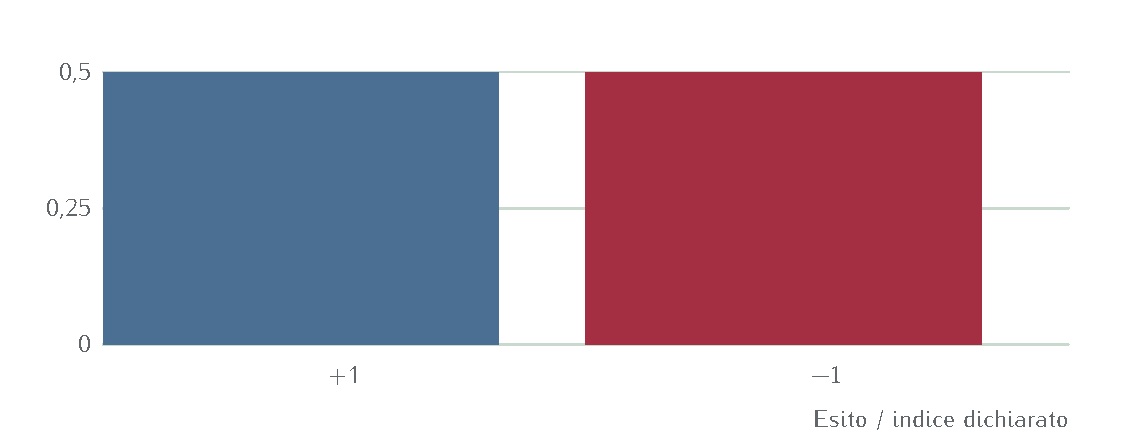
\includegraphics[width=\linewidth,height=94mm,keepaspectratio]{figure/f94e6a1a63cf0e52b.pdf}\FigureCaption{2.24 \(\cdot\) esempio 1 \(\cdot\) Probabilità della misura \(X\)}\end{FigureBlock}
\begin{FigureBlock}\begin{minipage}[t]{.485\linewidth}\centering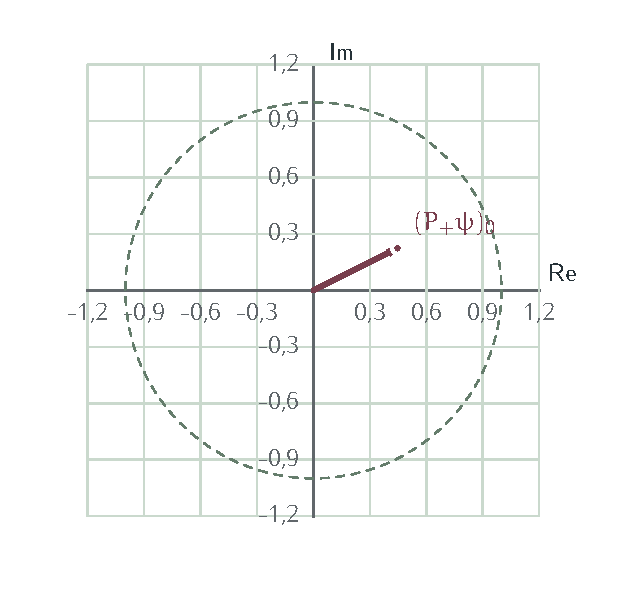
\includegraphics[width=\linewidth,height=63mm,keepaspectratio]{figure/f3a4e0457c0f8492f.pdf}\par{\sffamily\footnotesize \((P_{+}\psi )_{0}\)\par}\end{minipage}\hfill\begin{minipage}[t]{.485\linewidth}\centering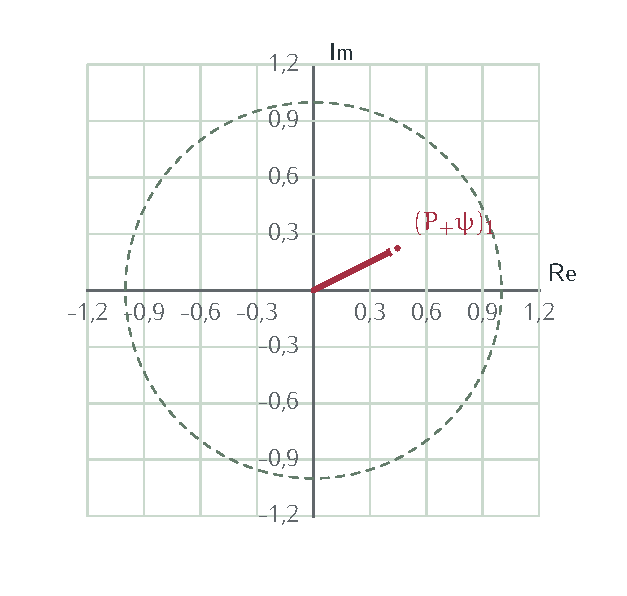
\includegraphics[width=\linewidth,height=63mm,keepaspectratio]{figure/f0fd32fa925246bea.pdf}\par{\sffamily\footnotesize \((P_{+}\psi )_{1}\)\par}\end{minipage}\FigureCaption{2.24 \(\cdot\) esempio 1 \(\cdot\) Componenti delle proiezioni in \(C^{2}\)}\end{FigureBlock}
\begin{FigureBlock}\begin{minipage}[t]{.485\linewidth}\centering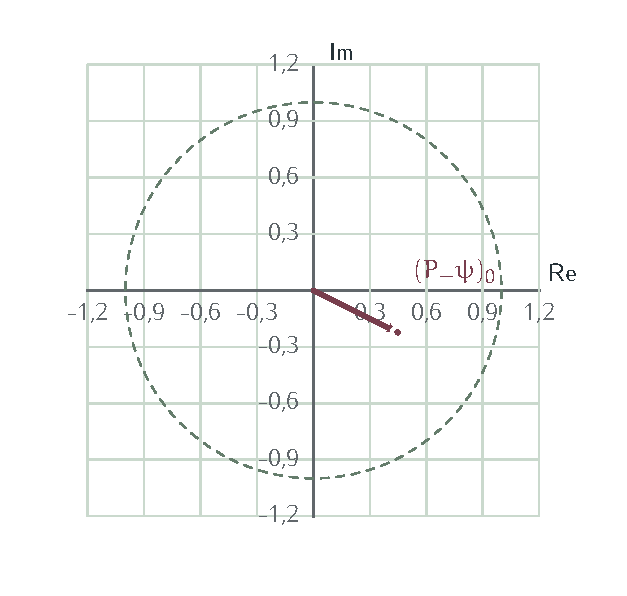
\includegraphics[width=\linewidth,height=63mm,keepaspectratio]{figure/f434ed061b4c28c55.pdf}\par{\sffamily\footnotesize \((P_{-}\psi )_{0}\)\par}\end{minipage}\hfill\begin{minipage}[t]{.485\linewidth}\centering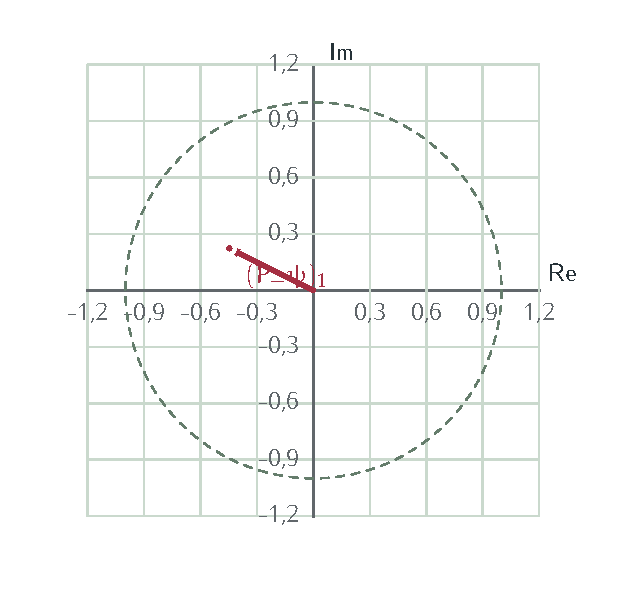
\includegraphics[width=\linewidth,height=63mm,keepaspectratio]{figure/fdd30b9247997190d.pdf}\par{\sffamily\footnotesize \((P_{-}\psi )_{1}\)\par}\end{minipage}\FigureCaption{2.24 \(\cdot\) esempio 1 \(\cdot\) Componenti delle proiezioni in \(C^{2}\)}\end{FigureBlock}
\begin{FigureBlock}\centering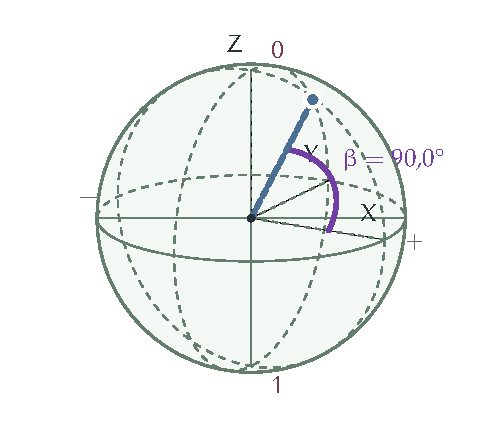
\includegraphics[width=\linewidth,height=94mm,keepaspectratio]{figure/f78d1121188874ff8.pdf}\FigureCaption{2.24 \(\cdot\) esempio 1 \(\cdot\) Stato iniziale e direzione +X della misura}\end{FigureBlock}
\begin{FigureBlock}\begin{minipage}[t]{.485\linewidth}\centering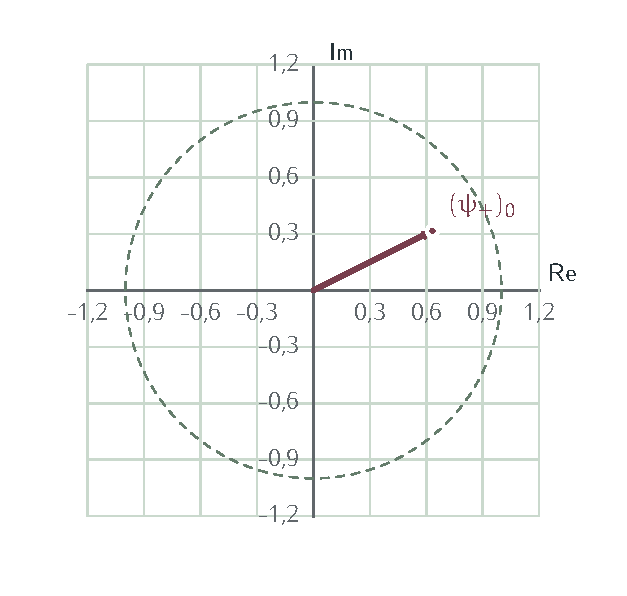
\includegraphics[width=\linewidth,height=63mm,keepaspectratio]{figure/f5631d0facb96cc4a.pdf}\par{\sffamily\footnotesize \((\psi _{+})_{0}\)\par}\end{minipage}\hfill\begin{minipage}[t]{.485\linewidth}\centering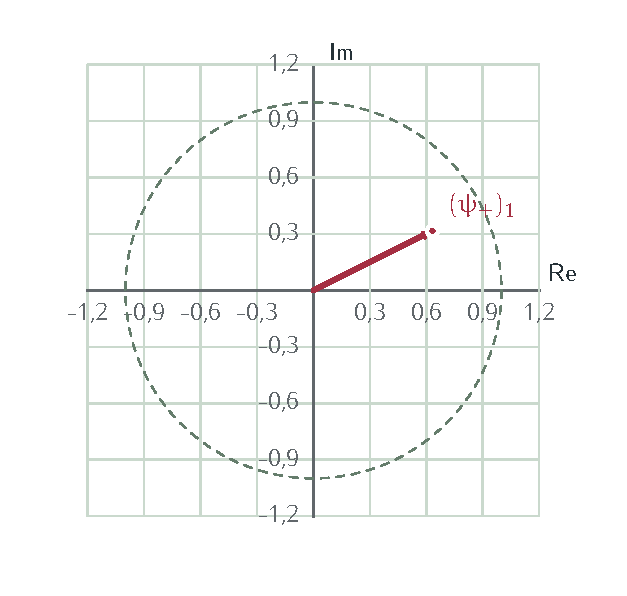
\includegraphics[width=\linewidth,height=63mm,keepaspectratio]{figure/f29c8856ca0cc89f3.pdf}\par{\sffamily\footnotesize \((\psi _{+})_{1}\)\par}\end{minipage}\FigureCaption{2.24 \(\cdot\) esempio 1 \(\cdot\) Stati condizionati dei due rami}\end{FigureBlock}
\begin{FigureBlock}\begin{minipage}[t]{.485\linewidth}\centering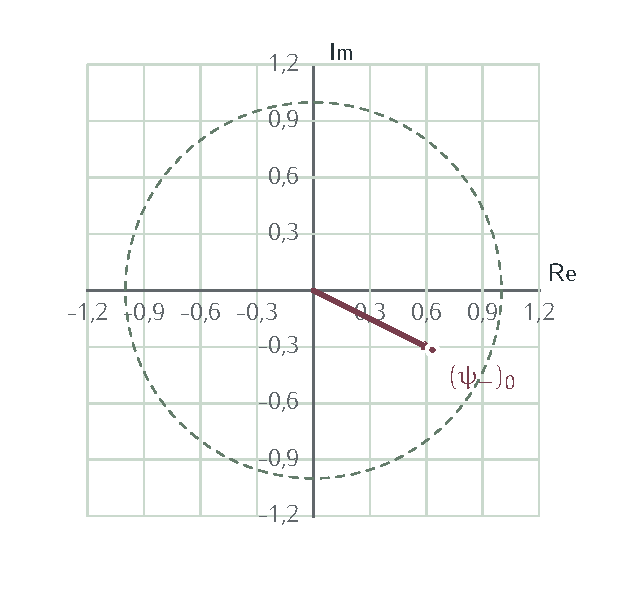
\includegraphics[width=\linewidth,height=63mm,keepaspectratio]{figure/fd9125b46a7a8850c.pdf}\par{\sffamily\footnotesize \((\psi _{-})_{0}\)\par}\end{minipage}\hfill\begin{minipage}[t]{.485\linewidth}\centering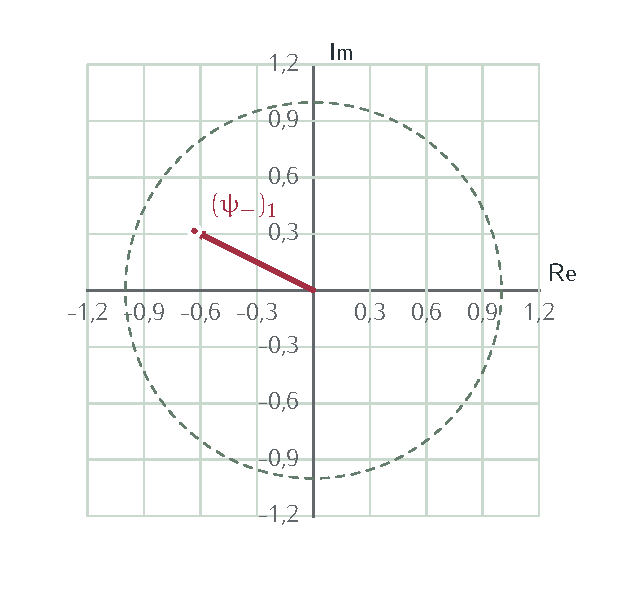
\includegraphics[width=\linewidth,height=63mm,keepaspectratio]{figure/f967a550d3cdf4cca.pdf}\par{\sffamily\footnotesize \((\psi _{-})_{1}\)\par}\end{minipage}\FigureCaption{2.24 \(\cdot\) esempio 1 \(\cdot\) Stati condizionati dei due rami}\end{FigureBlock}
\begin{FigureBlock}\begin{minipage}[t]{.485\linewidth}\centering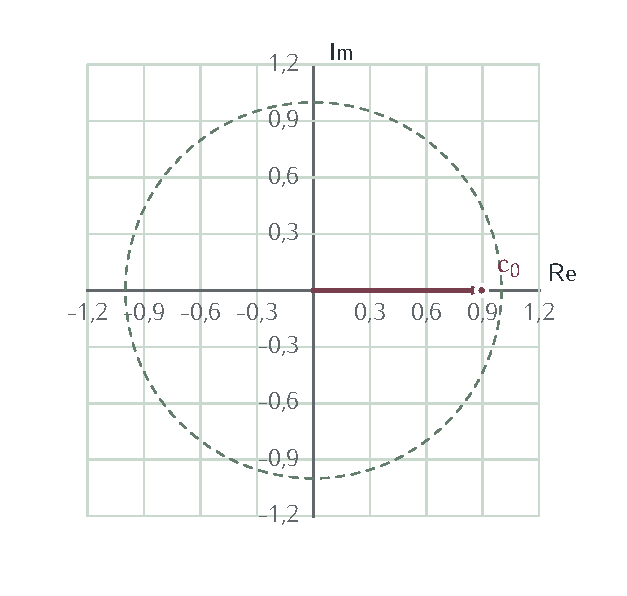
\includegraphics[width=\linewidth,height=63mm,keepaspectratio]{figure/f0364ff81b5e13f06.pdf}\par{\sffamily\footnotesize \(c_{0}\)\par}\end{minipage}\hfill\begin{minipage}[t]{.485\linewidth}\centering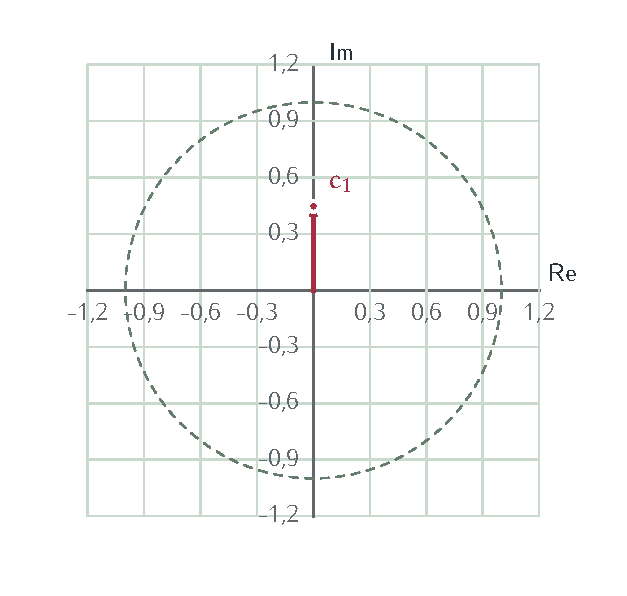
\includegraphics[width=\linewidth,height=63mm,keepaspectratio]{figure/f3671b82e02ed952e.pdf}\par{\sffamily\footnotesize \(c_{1}\)\par}\end{minipage}\FigureCaption{2.24 \(\cdot\) esempio 1 \(\cdot\) Componenti complesse}\end{FigureBlock}
\begin{FigureBlock}\centering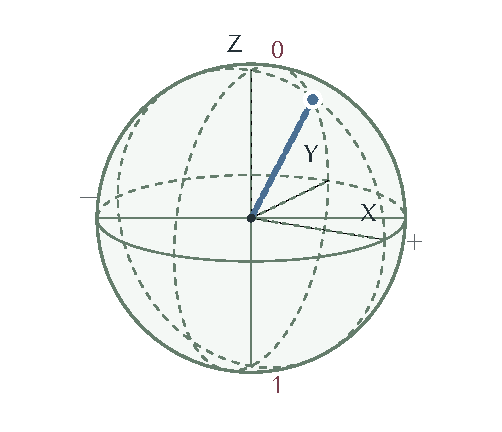
\includegraphics[width=\linewidth,height=94mm,keepaspectratio]{figure/fe3587a4d3c7cb4d0.pdf}\FigureCaption{2.24 \(\cdot\) esempio 1 \(\cdot\) Sfera di Bloch \(\cdot\) stato dell'esempio}\end{FigureBlock}

\phantomsection\label{c2-born-example-1-step-1}
\BookHeading{01 Dichiarare stato e base}

\MathBlock{03C8003D00280032002C006900291D40002F221A0035003B0020201603C8201600B2003D00280034002B00310029002F0035003D0031}{\psi =(2,\allowbreak i)^{T}/\sqrt{5};\allowbreak \ \Vert \psi \Vert ^{2}=(4+1)/5=1}
\MathBlock{0075208A003D00280031002C003100291D40002F221A0032003B00200075208B003D00280031002C2212003100291D40002F221A0032}{u_{+}=(1{,}1)^{T}/\sqrt{2};\allowbreak \ u_{-}=(1,\allowbreak - 1)^{T}/\sqrt{2}}

La base \(X\) è ortonormale; associamo gli esiti +1 e \(- 1\) ai suoi due vettori.\par


\phantomsection\label{c2-born-example-1-step-2}
\BookHeading{02 Calcolare le ampiezze}

\MathBlock{0061208A003D00280032002B00690029002F221A00310030003B00200061208B003D00280032221200690029002F221A00310030}{a_{+}=(2+i)/\sqrt{10};\allowbreak \ a_{-}=(2- i)/\sqrt{10}}

Il bra di ciascun vettore di base moltiplica il ket dello stato.\par


\phantomsection\label{c2-born-example-1-step-3}
\BookHeading{03 Passare ai moduli quadri}

\MathBlock{0070208A003D0028003200B2002B003100B20029002F00310030003D0031002F0032003B00200070208B003D0028003200B2002B002822120031002900B20029002F00310030003D0031002F0032}{p_{+}=(2^{2}+1^{2})/10=1/2;\allowbreak \ p_{-}=(2^{2}+(- 1)^{2})/10=1/2}

Le probabilità sono reali non negative e sommano a uno.\par


\phantomsection\label{c2-born-example-1-step-4}
\BookHeading{04 Costruire i vettori proiettati}

\MathBlock{0050208A03C8003D002800280032002B00690029002C00280032002B0069002900291D40002F00280032221A00350029}{P_{+}\psi =((2+i),\allowbreak (2+i))^{T}/(2\sqrt{5})}
\MathBlock{0050208B03C8003D002800280032221200690029002C002822120032002B0069002900291D40002F00280032221A00350029}{P_{-}\psi =((2- i),\allowbreak (- 2+i))^{T}/(2\sqrt{5})}
\MathBlock{0050208A03C8002B0050208B03C8003D00280032002C006900291D40002F221A0035}{P_{+}\psi +P_{-}\psi =(2,\allowbreak i)^{T}/\sqrt{5}}

I due vettori nello spazio \(C^{2}\) ricostruiscono lo stato iniziale. Le loro norme quadre sono le probabilità.\par


\phantomsection\label{c2-born-example-1-step-5}
\BookHeading{05 Normalizzare i rami possibili}

\MathBlock{03C8208A003D002800280032002B00690029002C00280032002B0069002900291D40002F221A00310030}{\psi _{+}=((2+i),\allowbreak (2+i))^{T}/\sqrt{10}}
\MathBlock{03C8208B003D002800280032221200690029002C002822120032002B0069002900291D40002F221A00310030}{\psi _{-}=((2- i),\allowbreak (- 2+i))^{T}/\sqrt{10}}
\MathBlock{201603C8208A201600B2003D201603C8208B201600B2003D0031}{\Vert \psi _{+}\Vert ^{2}=\Vert \psi _{-}\Vert ^{2}=1}

Una probabilità esattamente zero impedisce la divisione. Un valore positivo molto piccolo resta un evento possibile; i decimali visualizzati possono essere arrotondati.\par


\phantomsection\label{c2-born-example-1-step-6}
\BookHeading{06 Verificare dalla sfera di Bloch}

\MathBlock{0072003D00280030003B00200030002C0038003B00200030002C00360029003B0020006E0058003D00280031002C0030002C00300029003B0020007200B7006E0058003D0030}{r=(0;\allowbreak \ 0{,}8;\allowbreak \ 0{,}6);\allowbreak \ nX=(1{,}0{,}0);\allowbreak \ r\cdot nX=0}
\MathBlock{0070208A003D00280031002B007200B7006E00580029002F0032003D0031002F0032003B00200070208B003D002800312212007200B7006E00580029002F0032003D0031002F0032}{p_{+}=(1+r\cdot nX)/2=1/2;\allowbreak \ p_{-}=(1- r\cdot nX)/2=1/2}
\MathBlock{03B2003D0039003000B0003B00200070208A003D0063006F007300B2002803B2002F00320029003D0031002F0032}{\beta =90{}^{\circ} ;\allowbreak \ p_{+}=\cos ^{2}(\beta /2)=1/2}

L'angolo \(\beta \) è fra due direzioni di Bloch. Un angolo retto sulla sfera dà probabilità 1/2; due stati ortogonali corrispondono invece a punti antipodali.\par


\BookHeading{Interpretazione}

Le fasi dei due coefficienti di proiezione sono diverse, ma i moduli quadri sono entrambi 1/2. I due rami condizionati rappresentano i punti +X e \(- X\) della sfera.\par


\Needspace{.36\textheight}\phantomsection\label{c2-born-example-2}
{\sffamily\small\color{Accent} ESEMPIO SVOLTO 2\par}
\BookHeading{Preparazione allineata: esito certo e ramo nullo}
Dati \(\psi =|+\rangle \) e misura nella base \(X=\{|+\rangle ,\allowbreak |- \rangle \}\), con esiti +1 e \(- 1\).\par


\BookHeading{Geometria e configurazione dell'esempio}
\begin{FigureBlock}\centering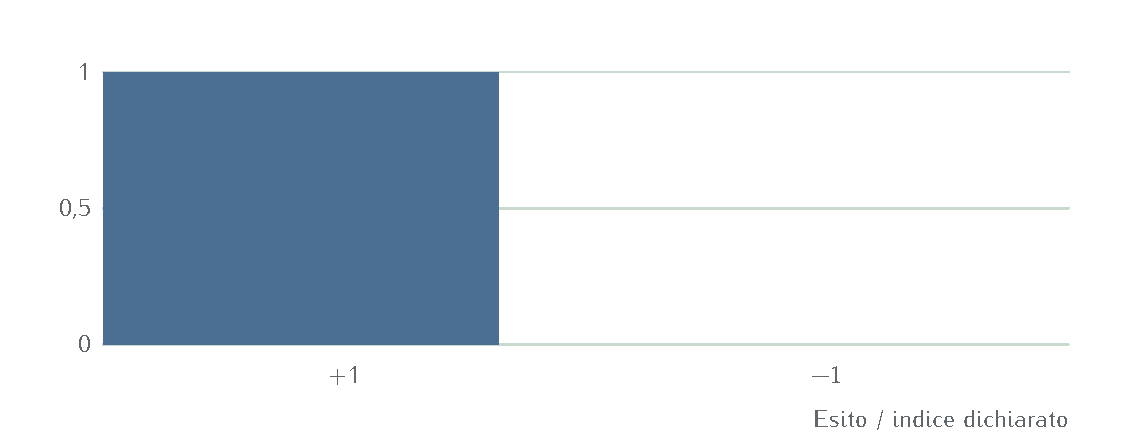
\includegraphics[width=\linewidth,height=94mm,keepaspectratio]{figure/f87281cdbb23ef260.pdf}\FigureCaption{2.24 \(\cdot\) esempio 2 \(\cdot\) Probabilità della misura \(X\)}\end{FigureBlock}
\begin{FigureBlock}\begin{minipage}[t]{.485\linewidth}\centering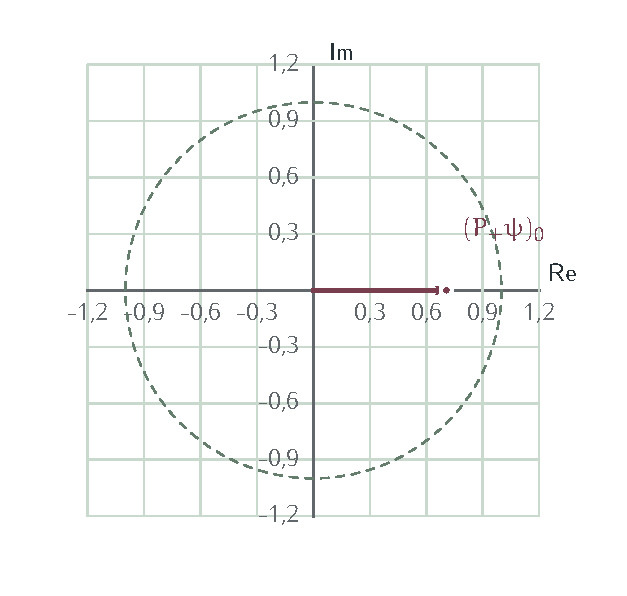
\includegraphics[width=\linewidth,height=63mm,keepaspectratio]{figure/fa9c5213f24866f2e.pdf}\par{\sffamily\footnotesize \((P_{+}\psi )_{0}\)\par}\end{minipage}\hfill\begin{minipage}[t]{.485\linewidth}\centering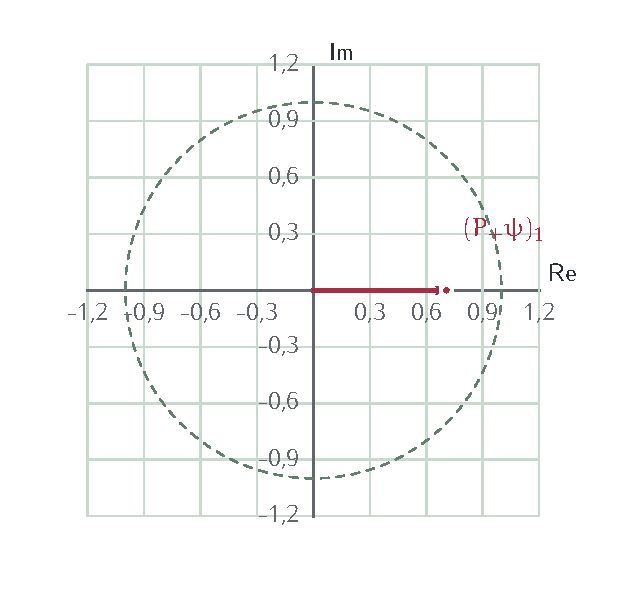
\includegraphics[width=\linewidth,height=63mm,keepaspectratio]{figure/f97d19bce86f6cf1c.pdf}\par{\sffamily\footnotesize \((P_{+}\psi )_{1}\)\par}\end{minipage}\FigureCaption{2.24 \(\cdot\) esempio 2 \(\cdot\) Componenti delle proiezioni in \(C^{2}\)}\end{FigureBlock}
\begin{FigureBlock}\begin{minipage}[t]{.485\linewidth}\centering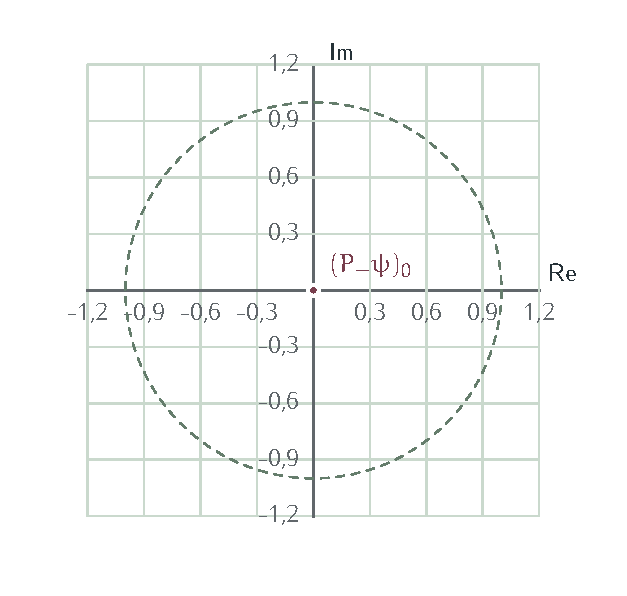
\includegraphics[width=\linewidth,height=63mm,keepaspectratio]{figure/fb56a8df1830ce1c1.pdf}\par{\sffamily\footnotesize \((P_{-}\psi )_{0}\)\par}\end{minipage}\hfill\begin{minipage}[t]{.485\linewidth}\centering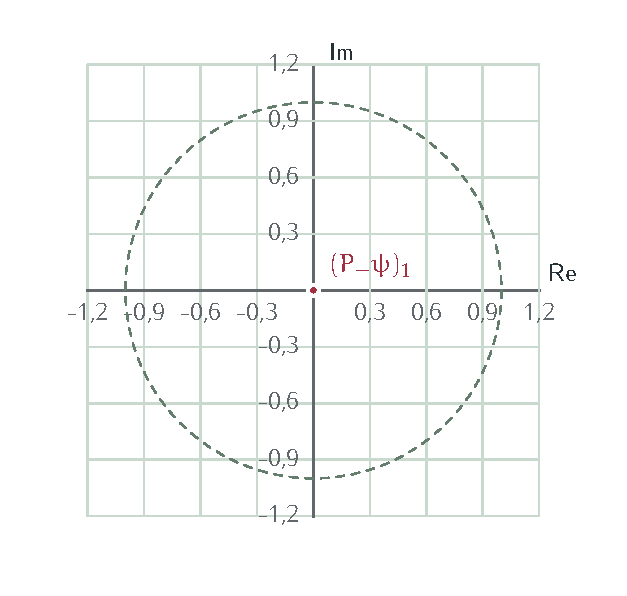
\includegraphics[width=\linewidth,height=63mm,keepaspectratio]{figure/f6c6e950501bec5ad.pdf}\par{\sffamily\footnotesize \((P_{-}\psi )_{1}\)\par}\end{minipage}\FigureCaption{2.24 \(\cdot\) esempio 2 \(\cdot\) Componenti delle proiezioni in \(C^{2}\)}\end{FigureBlock}
\begin{FigureBlock}\centering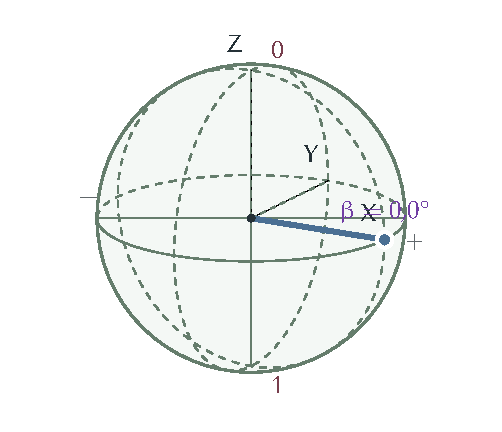
\includegraphics[width=\linewidth,height=94mm,keepaspectratio]{figure/fe893e2261705d2cc.pdf}\FigureCaption{2.24 \(\cdot\) esempio 2 \(\cdot\) Stato iniziale e direzione +X della misura}\end{FigureBlock}
\begin{FigureBlock}\begin{minipage}[t]{.485\linewidth}\centering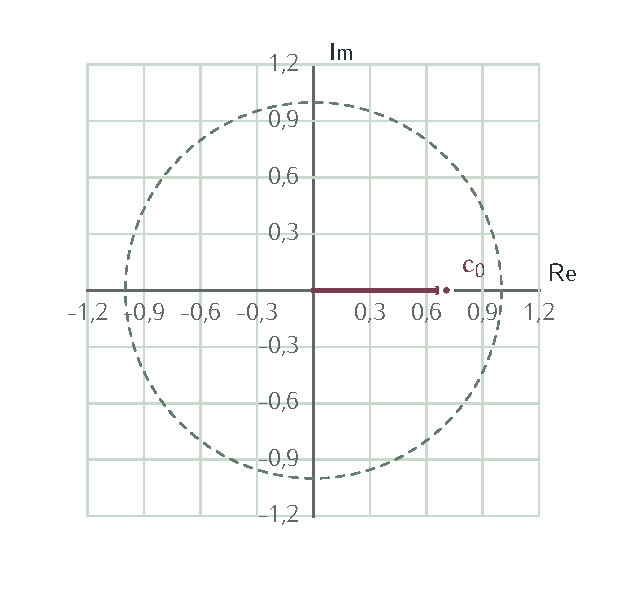
\includegraphics[width=\linewidth,height=63mm,keepaspectratio]{figure/fbed81334a6fd2acf.pdf}\par{\sffamily\footnotesize \(c_{0}\)\par}\end{minipage}\hfill\begin{minipage}[t]{.485\linewidth}\centering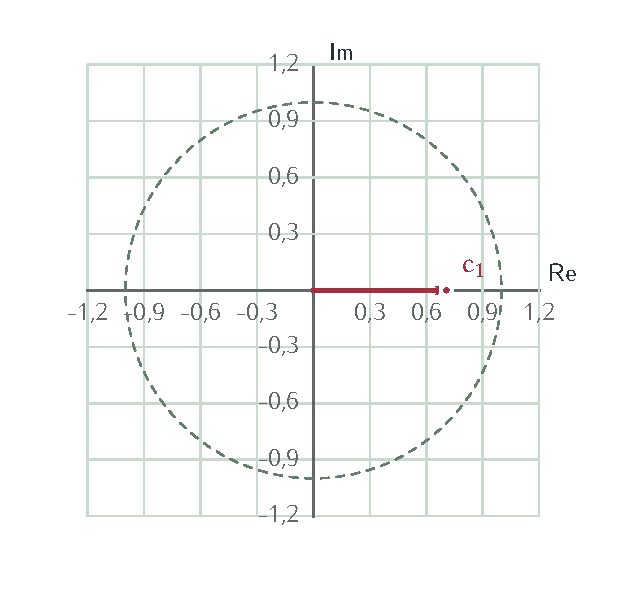
\includegraphics[width=\linewidth,height=63mm,keepaspectratio]{figure/fe1653d2d750bef8e.pdf}\par{\sffamily\footnotesize \(c_{1}\)\par}\end{minipage}\FigureCaption{2.24 \(\cdot\) esempio 2 \(\cdot\) Componenti complesse}\end{FigureBlock}
\begin{FigureBlock}\centering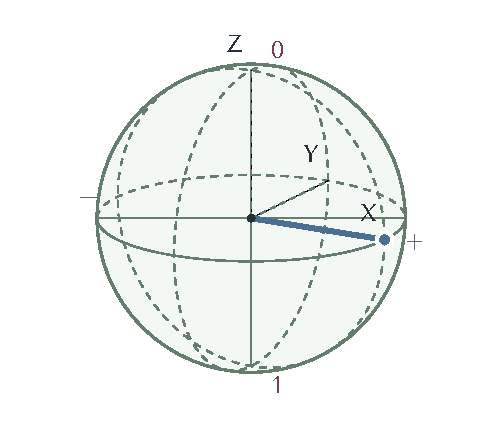
\includegraphics[width=\linewidth,height=94mm,keepaspectratio]{figure/f82d7f056487f5570.pdf}\FigureCaption{2.24 \(\cdot\) esempio 2 \(\cdot\) Sfera di Bloch \(\cdot\) stato dell'esempio}\end{FigureBlock}

\phantomsection\label{c2-born-example-2-step-1}
\BookHeading{01 Dichiarare stato e base}

\MathBlock{03C8003D007C002B27E9003D00280031002C003100291D40002F221A0032003B0020201603C8201600B2003D00280031002B00310029002F0032003D0031}{\psi =|+\rangle =(1{,}1)^{T}/\sqrt{2};\allowbreak \ \Vert \psi \Vert ^{2}=(1+1)/2=1}
\MathBlock{0075208A003D00280031002C003100291D40002F221A0032003B00200075208B003D00280031002C2212003100291D40002F221A0032}{u_{+}=(1{,}1)^{T}/\sqrt{2};\allowbreak \ u_{-}=(1,\allowbreak - 1)^{T}/\sqrt{2}}

La base \(X\) è ortonormale; associamo gli esiti +1 e \(- 1\) ai suoi due vettori.\par


\phantomsection\label{c2-born-example-2-step-2}
\BookHeading{02 Calcolare le ampiezze}

\MathBlock{0061208A003D00280031002B00310029002F0032003D0031003B00200061208B003D00280031221200310029002F0032003D0030}{a_{+}=(1+1)/2=1;\allowbreak \ a_{-}=(1- 1)/2=0}

Il bra di ciascun vettore di base moltiplica il ket dello stato.\par


\phantomsection\label{c2-born-example-2-step-3}
\BookHeading{03 Passare ai moduli quadri}

\MathBlock{0070208A003D007C0031007C00B2003D0031003B00200070208B003D007C0030007C00B2003D0030}{p_{+}=|1|^{2}=1;\allowbreak \ p_{-}=|0|^{2}=0}

Le probabilità sono reali non negative e sommano a uno.\par


\phantomsection\label{c2-born-example-2-step-4}
\BookHeading{04 Costruire i vettori proiettati}

\MathBlock{0050208A03C8003D0061208A0075208A003D03C8003B00200050208B03C8003D0061208B0075208B003D0030}{P_{+}\psi =a_{+}u_{+}=\psi ;\allowbreak \ P_{-}\psi =a_{-}u_{-}=0}

I due vettori nello spazio \(C^{2}\) ricostruiscono lo stato iniziale. Le loro norme quadre sono le probabilità.\par


\phantomsection\label{c2-born-example-2-step-5}
\BookHeading{05 Normalizzare i rami possibili}

\MathBlock{03C8208A003D0050208A03C8002F221A0031003D03C8}{\psi _{+}=P_{+}\psi /\sqrt{1}=\psi }
\MathBlock{0070208B003D0030003A00200069006C002000720061006D006F00202212002000E800200069006D0070006F00730073006900620069006C0065002000650020006E006F006E00200070006F00730073006900650064006500200075006E006F00200073007400610074006F00200063006F006E00640069007A0069006F006E00610074006F}{p_{-}=0:\ \text{il}\ \text{ramo}\ - \ \text{è}\ \text{impossibile}\ e\ \text{non}\ \text{possiede}\ \text{uno}\ \text{stato}\ \text{condizionato}}

Una probabilità esattamente zero impedisce la divisione. Un valore positivo molto piccolo resta un evento possibile; i decimali visualizzati possono essere arrotondati.\par


\phantomsection\label{c2-born-example-2-step-6}
\BookHeading{06 Verificare dalla sfera di Bloch}

\MathBlock{0072003D00280031003B00200030003B002000300029003B0020006E0058003D00280031002C0030002C00300029003B0020007200B7006E0058003D0031}{r=(1;\allowbreak \ 0;\allowbreak \ 0);\allowbreak \ nX=(1{,}0{,}0);\allowbreak \ r\cdot nX=1}
\MathBlock{0070208A003D00280031002B007200B7006E00580029002F0032003D0031003B00200070208B003D002800312212007200B7006E00580029002F0032003D0030}{p_{+}=(1+r\cdot nX)/2=1;\allowbreak \ p_{-}=(1- r\cdot nX)/2=0}
\MathBlock{03B2003D003000B0003B00200070208A003D0063006F007300B2002803B2002F00320029003D0031}{\beta =0{}^{\circ} ;\allowbreak \ p_{+}=\cos ^{2}(\beta /2)=1}

L'angolo \(\beta \) è fra due direzioni di Bloch. Un angolo retto sulla sfera dà probabilità 1/2; due stati ortogonali corrispondono invece a punti antipodali.\par


\BookHeading{Interpretazione}

La misura \(X\) conserva \(|+\rangle \) con probabilità uno. Il proiettore ortogonale restituisce il vettore nullo, che non può essere normalizzato.\par


\Needspace{7\baselineskip}
\BookHeading{Il passaggio successivo}
La misura separa rami e richiede un aggiornamento condizionato. Studieremo ora trasformazioni unitarie che conservano insieme tutte le ampiezze e la norma.\par


\Needspace{.43\textheight}
\section{Trasformare le ampiezze}
\phantomsection\label{c2-unitarie}

{\sffamily\small\color{Ink!70} Riferimento alle slide: p. 354.\par}

{\sffamily\small\color{Ink!70} Laboratorio locale: \nolinkurl{index.html#capitolo-2/unitarie}\par}

\BookHeading{Definizioni e costruzione}
Una porta unitaria opera linearmente sulle ampiezze. Calcoliamo ogni componente in uscita e verifichiamo che la norma resti uno.\par

Una trasformazione unitaria descrive un'evoluzione ideale reversibile del sistema considerato. La relazione \(U{}^{\dagger} U=I\) garantisce la conservazione di tutti i prodotti interni, e quindi della normalizzazione e della distinguibilità fra stati ortogonali.\par

Il prodotto matrice-vettore deve essere sviluppato sulle ampiezze complesse. Cambi di segno e fattori immaginari possono lasciare invariati alcuni moduli e modificare le interferenze successive. Per questo conserviamo le componenti complete anche quando mostriamo un grafico delle probabilità.\par


\MathBlock{03C82032003D005503C8003B0020201603C82032201600B2003D27E803C8007C005520200055007C03C827E9003D0031002E}{\psi {}^{\prime} =U\psi ;\allowbreak \ \Vert \psi {}^{\prime} \Vert ^{2}=\langle \psi |U{}^{\dagger} U|\psi \rangle =1.}

\BookHeading{Come leggere le figure}
Piani delle componenti; l'unitarietà conserva la norma nello spazio complesso.\par


\Needspace{.36\textheight}\phantomsection\label{c2-unitarie-example-1}
{\sffamily\small\color{Accent} ESEMPIO SVOLTO 1\par}
\BookHeading{Hadamard e scambio degli assi X/Z}
Dati \(\psi =(2,\allowbreak i)^{T}/\sqrt{5}\) e \(H=(1/\sqrt{2})\)\(\begin{pmatrix}1&1\\1&- 1\end{pmatrix}\).\par


\BookHeading{Geometria e configurazione dell'esempio}
\begin{FigureBlock}\centering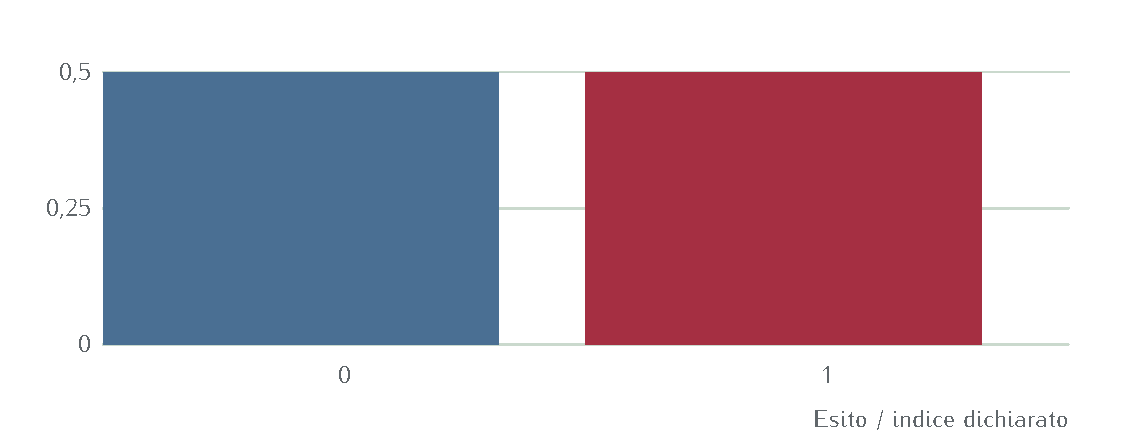
\includegraphics[width=\linewidth,height=94mm,keepaspectratio]{figure/f2366a7ed34a1b285.pdf}\FigureCaption{2.25 \(\cdot\) esempio 1 \(\cdot\) Probabilità \(Z\) dopo la trasformazione}\end{FigureBlock}
\begin{FigureBlock}\begin{minipage}[t]{.485\linewidth}\centering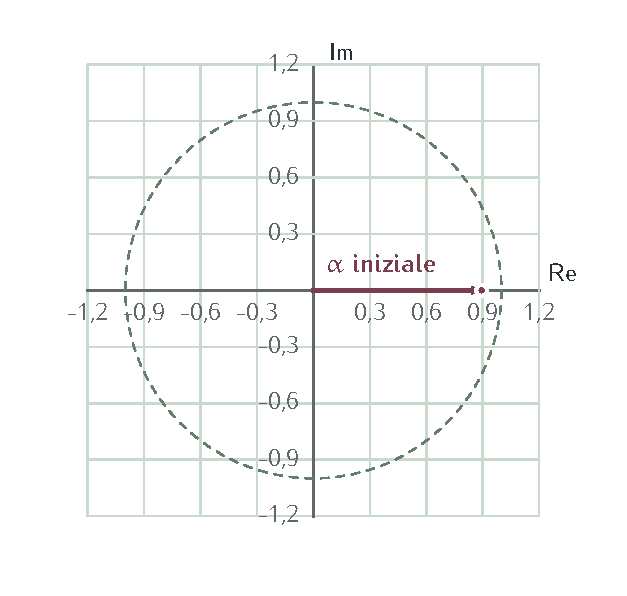
\includegraphics[width=\linewidth,height=63mm,keepaspectratio]{figure/f07b9137c9393f657.pdf}\par{\sffamily\footnotesize \(\alpha \) iniziale\par}\end{minipage}\hfill\begin{minipage}[t]{.485\linewidth}\centering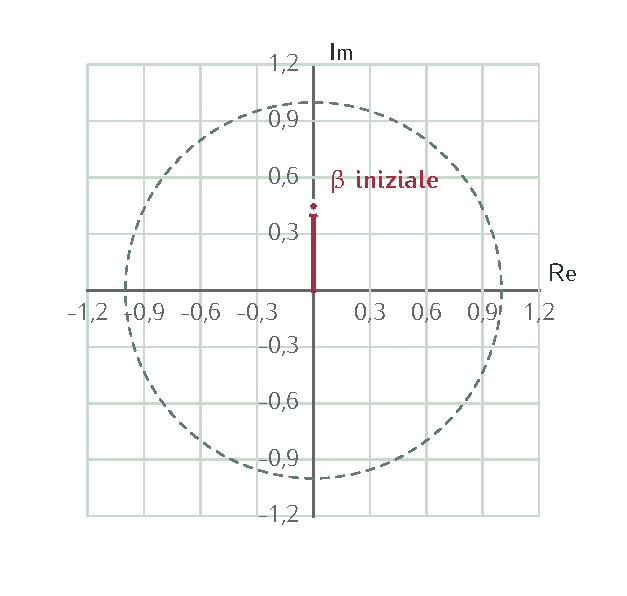
\includegraphics[width=\linewidth,height=63mm,keepaspectratio]{figure/fbe2ea2958012628a.pdf}\par{\sffamily\footnotesize \(\beta \) iniziale\par}\end{minipage}\FigureCaption{2.25 \(\cdot\) esempio 1 \(\cdot\) Componenti iniziali e finali}\end{FigureBlock}
\begin{FigureBlock}\begin{minipage}[t]{.485\linewidth}\centering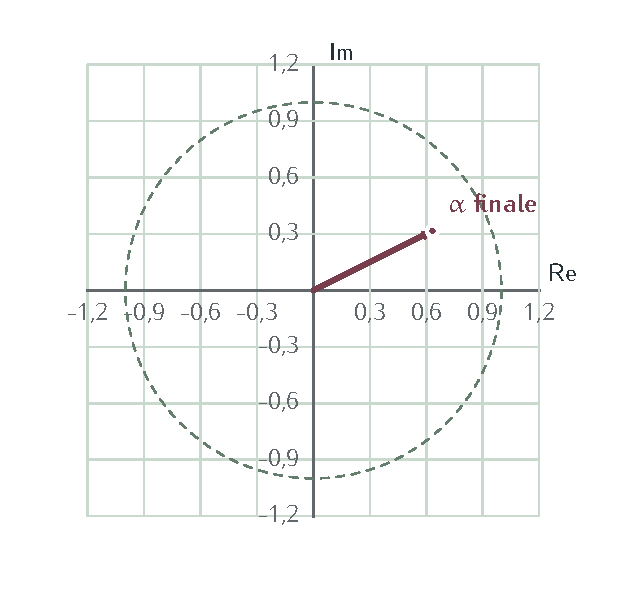
\includegraphics[width=\linewidth,height=63mm,keepaspectratio]{figure/f6a97867a39a52d70.pdf}\par{\sffamily\footnotesize \(\alpha \) finale\par}\end{minipage}\hfill\begin{minipage}[t]{.485\linewidth}\centering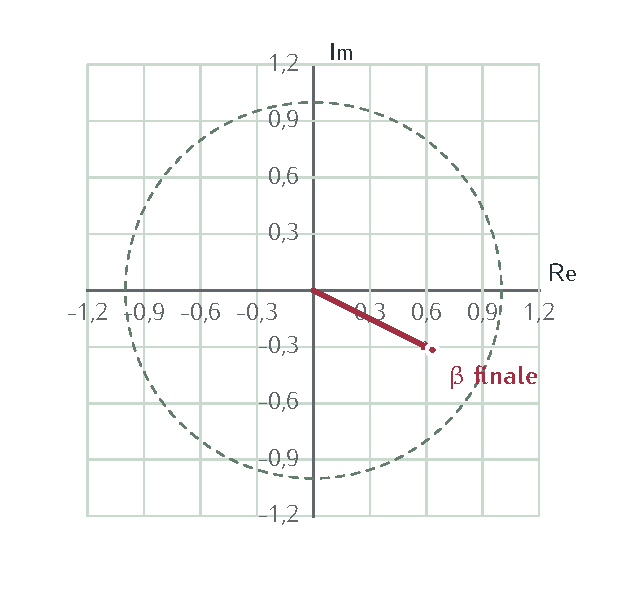
\includegraphics[width=\linewidth,height=63mm,keepaspectratio]{figure/f60b3e7db995fb993.pdf}\par{\sffamily\footnotesize \(\beta \) finale\par}\end{minipage}\FigureCaption{2.25 \(\cdot\) esempio 1 \(\cdot\) Componenti iniziali e finali}\end{FigureBlock}
\begin{FigureBlock}\centering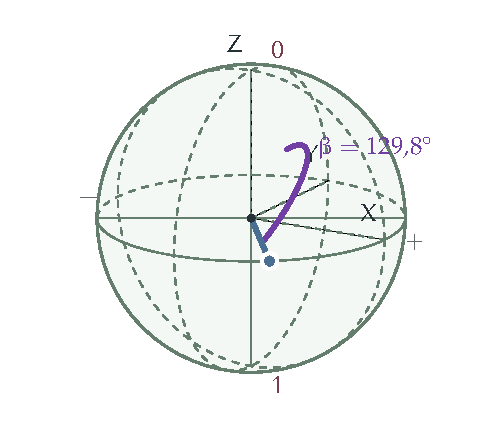
\includegraphics[width=\linewidth,height=94mm,keepaspectratio]{figure/f57a6964f799169c7.pdf}\FigureCaption{2.25 \(\cdot\) esempio 1 \(\cdot\) Confronto Bloch: stato finale e riferimento iniziale}\end{FigureBlock}
\begin{FigureBlock}\begin{minipage}[t]{.485\linewidth}\centering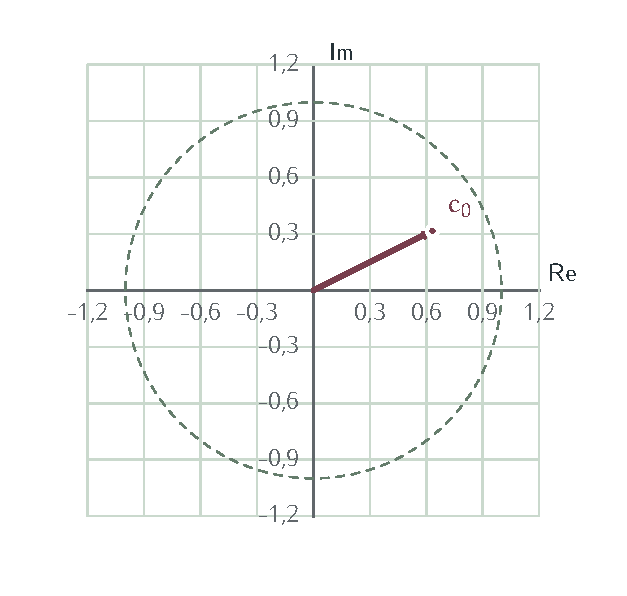
\includegraphics[width=\linewidth,height=63mm,keepaspectratio]{figure/f09274621f415f5ff.pdf}\par{\sffamily\footnotesize \(c_{0}\)\par}\end{minipage}\hfill\begin{minipage}[t]{.485\linewidth}\centering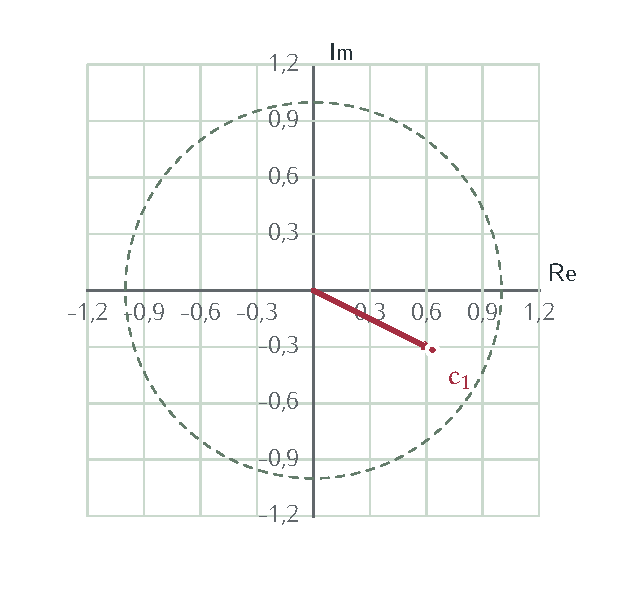
\includegraphics[width=\linewidth,height=63mm,keepaspectratio]{figure/fc1b41fdf7d062ada.pdf}\par{\sffamily\footnotesize \(c_{1}\)\par}\end{minipage}\FigureCaption{2.25 \(\cdot\) esempio 1 \(\cdot\) Componenti complesse}\end{FigureBlock}
\begin{FigureBlock}\centering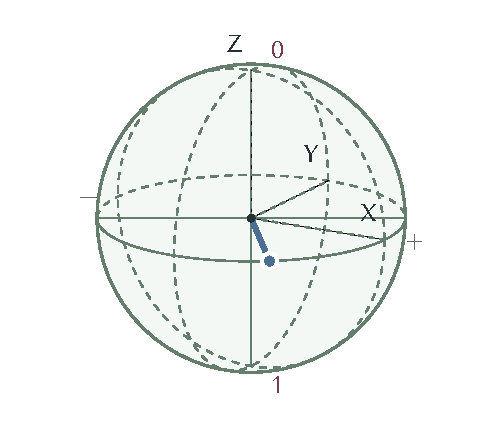
\includegraphics[width=\linewidth,height=94mm,keepaspectratio]{figure/f32b83906d730dfa5.pdf}\FigureCaption{2.25 \(\cdot\) esempio 1 \(\cdot\) Sfera di Bloch \(\cdot\) stato dell'esempio}\end{FigureBlock}

\phantomsection\label{c2-unitarie-example-1-step-1}
\BookHeading{01 Dichiarare l'operatore esatto}

\MathBlock{0055003D0048003D00280031002F221A00320029005B005B0031002C0031005D002C005B0031002C22120031005D005D003B002000482020003D0048}{U=H=(1/\sqrt{2})\begin{pmatrix}1&1\\1&- 1\end{pmatrix};\allowbreak \ H{}^{\dagger} =H}

Le matrici agiscono sulla base canonica \(|0\rangle ,\allowbreak |1\rangle \) e mantengono le ampiezze complesse.\par


\phantomsection\label{c2-unitarie-example-1-step-2}
\BookHeading{02 Verificare l'unitarietà}

\MathBlock{004820200048003D00280031002F00320029005B005B0031002B0031002C003122120031005D002C005B003122120031002C0031002B0031005D005D003D0049}{H{}^{\dagger} H=(1/2)\begin{pmatrix}1+1&1- 1\\1- 1&1+1\end{pmatrix}=I}

I prodotti sulle diagonali valgono uno e quelli fuori diagonale zero.\par


\phantomsection\label{c2-unitarie-example-1-step-3}
\BookHeading{03 Moltiplicare riga per colonna}

\MathBlock{004803C8003D002800280032002B00690029002C0028003222120069002900291D40002F221A00310030}{H\psi =((2+i),\allowbreak (2- i))^{T}/\sqrt{10}}

La prima riga fornisce la nuova componente 0 e la seconda la nuova componente 1.\par


\phantomsection\label{c2-unitarie-example-1-step-4}
\BookHeading{04 Controllare la norma in uscita}

\MathBlock{2016004803C8201600B2003D0028007C0032002B0069007C00B2002B007C003222120069007C00B20029002F00310030003D00280035002B00350029002F00310030003D0031}{\Vert H\psi \Vert ^{2}=(|2+i|^{2}+|2- i|^{2})/10=(5+5)/10=1}

La conservazione verificata su questo stato è conseguenza dell'identità \(U{}^{\dagger} U=I\) valida per ogni ingresso.\par


\phantomsection\label{c2-unitarie-example-1-step-5}
\BookHeading{05 Confrontare i punti di Bloch}

\MathBlock{007200200069006E0069007A00690061006C0065003D00280030003B00200030002C0038003B00200030002C00360029003B00200072002000660069006E0061006C0065003D00280030002C0036003B0020002D0030002C0038003B002000300029}{r\ \text{iniziale}=(0;\allowbreak \ 0{,}8;\allowbreak \ 0{,}6);\allowbreak \ r\ \text{finale}=(0{,}6;\allowbreak \ -0{,}8;\allowbreak \ 0)}
\MathBlock{002800722093002C00721D67002C0072D835DCCF002921A600280072D835DCCF002C221200721D67002C007220930029}{(r_{x},\allowbreak r_{y},\allowbreak r_{z})\mapsto (r_{z},\allowbreak - r_{y},\allowbreak r_{x})}

Hadamard scambia le coordinate x e z e inverte y: equivale a una rotazione di \(180{}^{\circ} \) attorno all'asse \((1{,}0{,}1)/\sqrt{2}\), a meno di una fase globale del ket.\par


\phantomsection\label{c2-unitarie-example-1-step-6}
\BookHeading{06 Applicare l'inversa}

\MathBlock{00480028004803C80029003D00280031002F221A00320030002900280034002C0032006900291D40003D00280032002C006900291D40002F221A0035003D03C8}{H(H\psi )=(1/\sqrt{20})(4{,}2i)^{T}=(2,\allowbreak i)^{T}/\sqrt{5}=\psi }

Il secondo calcolo ripristina esattamente l'ingresso.\par


\BookHeading{Interpretazione}

Il punto (0,4/5,3/5) diventa \((3/5,\allowbreak - 4/5{,}0)\). Le probabilità \(Z\) finali sono uniformi e l'inversa \(H\) ripristina la preparazione.\par


\Needspace{.36\textheight}\phantomsection\label{c2-unitarie-example-2}
{\sffamily\small\color{Accent} ESEMPIO SVOLTO 2\par}
\BookHeading{Porta di fase e rotazione attorno a \(Z\)}
Dati \(\psi =|+\rangle =(1{,}1)^{T}/\sqrt{2}\), \(U=\operatorname{diag}(1,\allowbreak i)\).\par


\BookHeading{Geometria e configurazione dell'esempio}
\begin{FigureBlock}\centering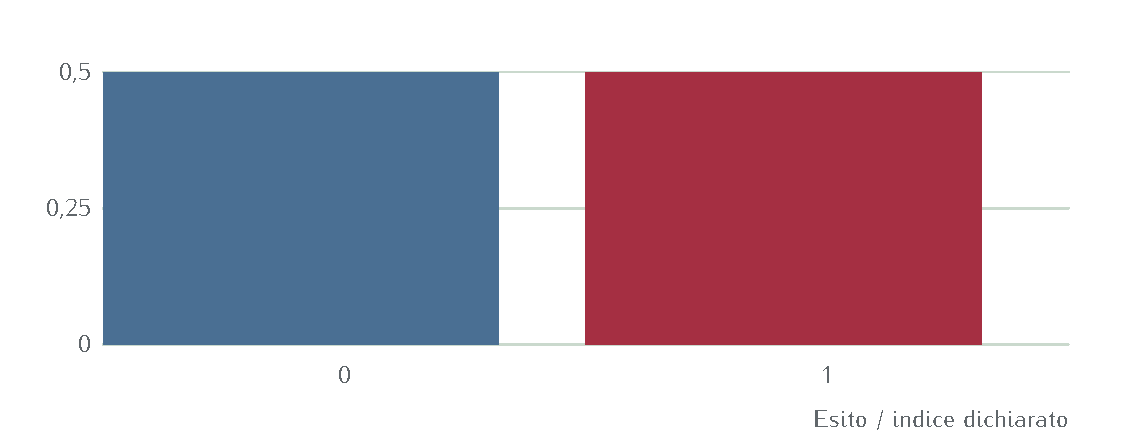
\includegraphics[width=\linewidth,height=94mm,keepaspectratio]{figure/f2366a7ed34a1b285.pdf}\FigureCaption{2.25 \(\cdot\) esempio 2 \(\cdot\) Probabilità \(Z\) dopo la trasformazione}\end{FigureBlock}
\begin{FigureBlock}\begin{minipage}[t]{.485\linewidth}\centering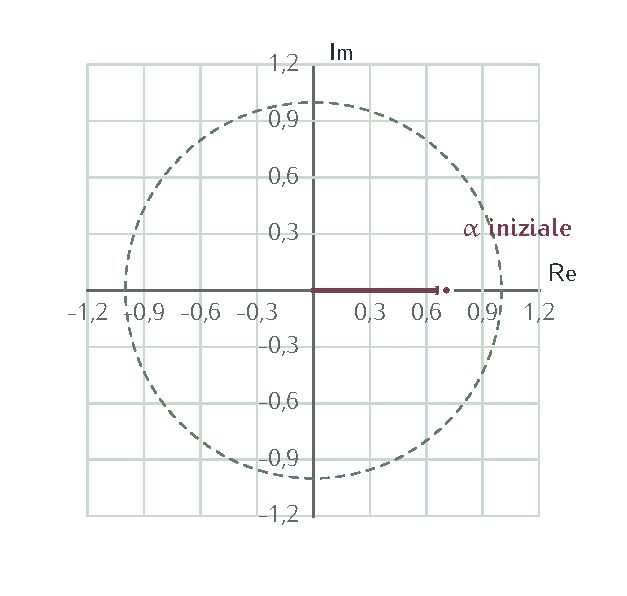
\includegraphics[width=\linewidth,height=63mm,keepaspectratio]{figure/f1a7add696bc1c39b.pdf}\par{\sffamily\footnotesize \(\alpha \) iniziale\par}\end{minipage}\hfill\begin{minipage}[t]{.485\linewidth}\centering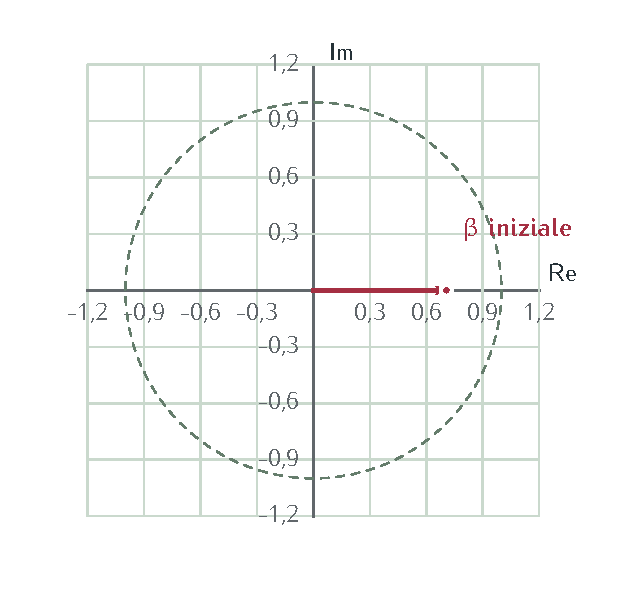
\includegraphics[width=\linewidth,height=63mm,keepaspectratio]{figure/f7af65ff7e0e5e151.pdf}\par{\sffamily\footnotesize \(\beta \) iniziale\par}\end{minipage}\FigureCaption{2.25 \(\cdot\) esempio 2 \(\cdot\) Componenti iniziali e finali}\end{FigureBlock}
\begin{FigureBlock}\begin{minipage}[t]{.485\linewidth}\centering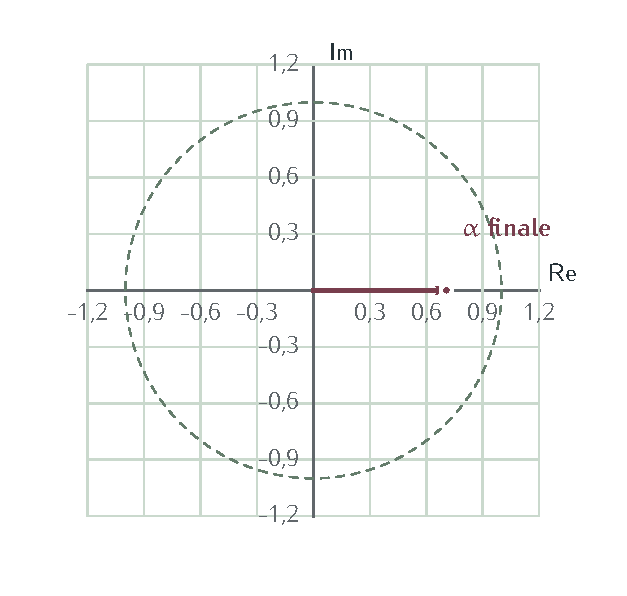
\includegraphics[width=\linewidth,height=63mm,keepaspectratio]{figure/f0ba1a01df1975d79.pdf}\par{\sffamily\footnotesize \(\alpha \) finale\par}\end{minipage}\hfill\begin{minipage}[t]{.485\linewidth}\centering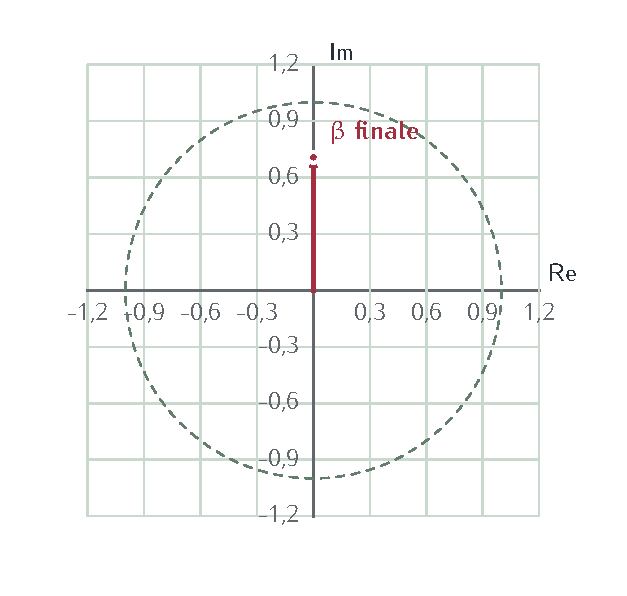
\includegraphics[width=\linewidth,height=63mm,keepaspectratio]{figure/fdde5e4da3295a1a2.pdf}\par{\sffamily\footnotesize \(\beta \) finale\par}\end{minipage}\FigureCaption{2.25 \(\cdot\) esempio 2 \(\cdot\) Componenti iniziali e finali}\end{FigureBlock}
\begin{FigureBlock}\centering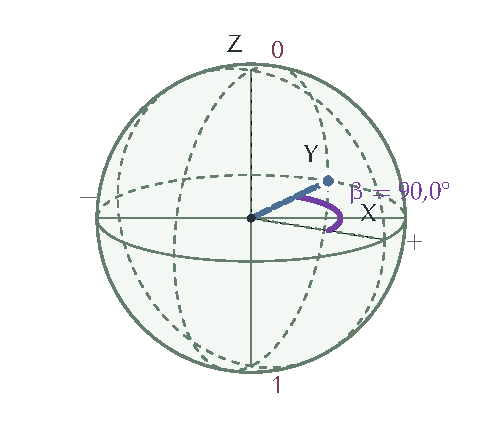
\includegraphics[width=\linewidth,height=94mm,keepaspectratio]{figure/f339f3fe8758a670f.pdf}\FigureCaption{2.25 \(\cdot\) esempio 2 \(\cdot\) Confronto Bloch: stato finale e riferimento iniziale}\end{FigureBlock}
\begin{FigureBlock}\begin{minipage}[t]{.485\linewidth}\centering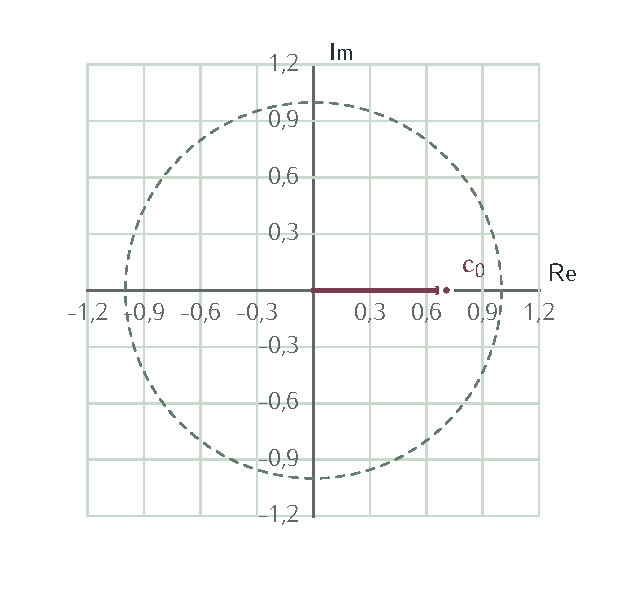
\includegraphics[width=\linewidth,height=63mm,keepaspectratio]{figure/fbed81334a6fd2acf.pdf}\par{\sffamily\footnotesize \(c_{0}\)\par}\end{minipage}\hfill\begin{minipage}[t]{.485\linewidth}\centering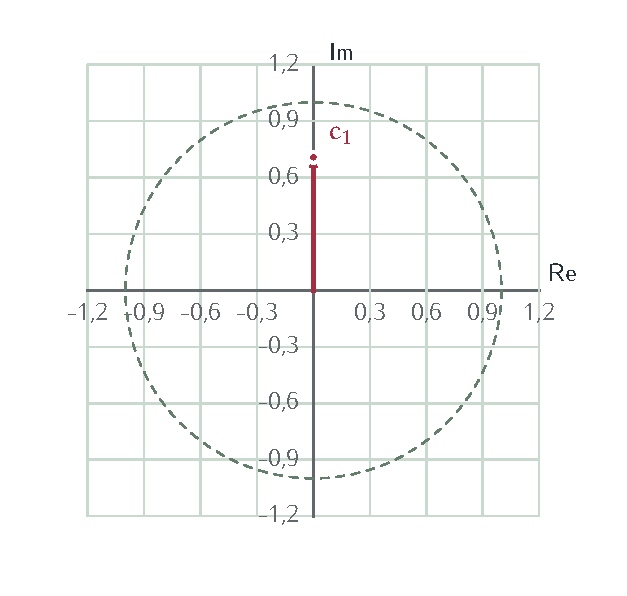
\includegraphics[width=\linewidth,height=63mm,keepaspectratio]{figure/f2bf9db3309b7c31a.pdf}\par{\sffamily\footnotesize \(c_{1}\)\par}\end{minipage}\FigureCaption{2.25 \(\cdot\) esempio 2 \(\cdot\) Componenti complesse}\end{FigureBlock}
\begin{FigureBlock}\centering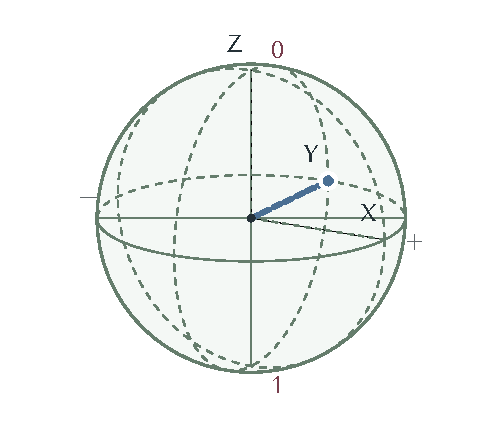
\includegraphics[width=\linewidth,height=94mm,keepaspectratio]{figure/fae21600cc1d0968b.pdf}\FigureCaption{2.25 \(\cdot\) esempio 2 \(\cdot\) Sfera di Bloch \(\cdot\) stato dell'esempio}\end{FigureBlock}

\phantomsection\label{c2-unitarie-example-2-step-1}
\BookHeading{01 Dichiarare l'operatore esatto}

\MathBlock{0055003D005B005B0031002C0030005D002C005B0030002C0069005D005D003B002000552020003D005B005B0031002C0030005D002C005B0030002C22120069005D005D}{U=\begin{pmatrix}1&0\\0&i\end{pmatrix};\allowbreak \ U{}^{\dagger} =\begin{pmatrix}1&0\\0&- i\end{pmatrix}}

Le matrici agiscono sulla base canonica \(|0\rangle ,\allowbreak |1\rangle \) e mantengono le ampiezze complesse.\par


\phantomsection\label{c2-unitarie-example-2-step-2}
\BookHeading{02 Verificare l'unitarietà}

\MathBlock{005520200055003D005B005B0031002C0030005D002C005B0030002C00282212006900290069005D005D003D0049}{U{}^{\dagger} U=\begin{pmatrix}1&0\\0&(- i)i\end{pmatrix}=I}

I prodotti sulle diagonali valgono uno e quelli fuori diagonale zero.\par


\phantomsection\label{c2-unitarie-example-2-step-3}
\BookHeading{03 Moltiplicare riga per colonna}

\MathBlock{0055007C002B27E9003D00280031002C006900291D40002F221A0032}{U|+\rangle =(1,\allowbreak i)^{T}/\sqrt{2}}

La prima riga fornisce la nuova componente 0 e la seconda la nuova componente 1.\par


\phantomsection\label{c2-unitarie-example-2-step-4}
\BookHeading{04 Controllare la norma in uscita}

\MathBlock{2016005503C8201600B2003D0028007C0031007C00B2002B007C0069007C00B20029002F0032003D0031}{\Vert U\psi \Vert ^{2}=(|1|^{2}+|i|^{2})/2=1}

La conservazione verificata su questo stato è conseguenza dell'identità \(U{}^{\dagger} U=I\) valida per ogni ingresso.\par


\phantomsection\label{c2-unitarie-example-2-step-5}
\BookHeading{05 Confrontare i punti di Bloch}

\MathBlock{007200200069006E0069007A00690061006C0065003D00280031003B00200030003B002000300029003B00200072002000660069006E0061006C0065003D00280030003B00200031003B002000300029}{r\ \text{iniziale}=(1;\allowbreak \ 0;\allowbreak \ 0);\allowbreak \ r\ \text{finale}=(0;\allowbreak \ 1;\allowbreak \ 0)}
\MathBlock{002800722093002C00721D67002C0072D835DCCF002921A60028221200721D67002C00722093002C0072D835DCCF0029}{(r_{x},\allowbreak r_{y},\allowbreak r_{z})\mapsto (- r_{y},\allowbreak r_{x},\allowbreak r_{z})}

Il fattore i sulla seconda componente aggiunge \(90{}^{\circ} \) alla fase relativa: sulla sfera è una rotazione di \(90{}^{\circ} \) attorno a \(Z\).\par


\phantomsection\label{c2-unitarie-example-2-step-6}
\BookHeading{06 Applicare l'inversa}

\MathBlock{0055202000280031002C006900291D40002F221A0032003D00280031002C0028221200690029006900291D40002F221A0032003D007C002B27E9}{U{}^{\dagger} (1,\allowbreak i)^{T}/\sqrt{2}=(1,\allowbreak (- i)i)^{T}/\sqrt{2}=|+\rangle }

Il secondo calcolo ripristina esattamente l'ingresso.\par


\BookHeading{Interpretazione}

Le probabilità \(Z\) restano uniformi mentre il punto di Bloch passa da +X a +Y. La porta agisce sulla fase relativa.\par


\Needspace{7\baselineskip}
\BookHeading{Il passaggio successivo}
Le trasformazioni unitarie cambiano la preparazione. Un'osservabile assegnerà valori numerici reali agli esiti e permetterà di calcolarne media e varianza.\par


% Authoritative exercise source. Preserve all derivations and diagrams.

\ExerciseStart{G2.12}{Preparare uno stato e renderne osservabile la fase}{Collegamento}

\BookHeading{Problema, dati e obiettivo}

Preparare \(\ket\psi=(\sqrt3/2)\ket0+(i/2)\ket1\). Calcolare bra, probabilità iniziali e stato dopo H. Confrontare con la preparazione a fase relativa nulla e con una moltiplicazione globale per \(e^{i\pi/4}\).

\ExTheory{\ExRef{c2-stati}{2.21}; \ExRef{c2-bra}{2.22}; \ExRef{c2-fase}{2.23}; \ExRef{c2-born}{2.24}; \ExRef{c2-unitarie}{2.25}}{Il bra è il coniugato trasposto del ket. La porta \(H=(1/\sqrt2)\begin{pmatrix}1&1\\1&-1\end{pmatrix}\) mescola le componenti. Per \(\alpha\ket0+\beta\ket1\), le coordinate di Bloch sono \((2\Re(\alpha^*\beta),2\Im(\alpha^*\beta),|\alpha|^2-|\beta|^2)\).}

\ExPrediction{La fase relativa è \(90^\circ\). La componente trasversale del vettore di Bloch è orientata lungo y; la Hadamard renderà equiprobabili le due uscite nella base Z.}

\ExFigure{\begin{tikzpicture}[>=Stealth,exlabel]
\node[left] at (-.3,0) {$ (\sqrt3,i)^T/2 $};\draw[Ink] (-.3,0)--(1.5,0);\node[draw=Accent,fill=white,minimum height=9mm,minimum width=10mm] at (0.5,0) {$ H $};\node[right] at (1.5,0) {$\ket{\psi_f}$};
\end{tikzpicture}}{La preparazione in ingresso ha ampiezze di moduli differenti.}


\begin{ExTasks}

\item Controllare la norma e scrivere il bra.

\item Calcolare le probabilità iniziali.

\item Eseguire i due prodotti riga-colonna con H.

\item Calcolare le probabilità finali e le coordinate di Bloch.

\item Ripetere per fase relativa nulla e giustificare l’invarianza rispetto alla fase globale.

\end{ExTasks}

\ExSolution

\ExStep{Bra e normalizzazione}

\ExEq{\bra\psi&=(\sqrt3/2,\ -i/2),\\\inner\psi\psi&=3/4+(-i)i/4=3/4+1/4=1.}

\ExStep{Lettura iniziale}

\(p_0=3/4\) e \(p_1=1/4\). Inoltre \(\alpha^*\beta=i\sqrt3/4\), quindi \(\mathbf r=(0,\sqrt3/2,1/2)\).

\ExStep{Applicare H}

\ExEq{H\ket\psi&=\frac1{2\sqrt2}\colv{\sqrt3+i\\\sqrt3-i},\\p'_0&=\frac{(\sqrt3-i)(\sqrt3+i)}8=\frac{3+1}8=\frac12,\\p'_1&=\frac{(\sqrt3+i)(\sqrt3-i)}8=\frac12.}

\ExStep{Controllare la geometria finale}

Le ampiezze finali danno
\ExEq{\alpha'^*\beta'&=(\sqrt3-i)^2/8=(2-2i\sqrt3)/8
=1/4-i\sqrt3/4,\\\mathbf r'&=(1/2,-\sqrt3/2,0).}
La norma del vettore di Bloch è \(1/4+3/4=1\); la quota finale nulla corrisponde a probabilità uguali.

\ExStep{Confrontare la fase relativa nulla}

Per \(\ket{\psi_0}=(\sqrt3,1)^T/2\), le ampiezze finali sono \((\sqrt3+1,\sqrt3-1)^T/(2\sqrt2)\). Quindi
\ExEq{p_0^{(0)}&=(\sqrt3+1)^2/8=(4+2\sqrt3)/8=\tfrac12+\tfrac{\sqrt3}{4},\\p_1^{(0)}&=\tfrac12-\tfrac{\sqrt3}{4}.}
I valori sono circa \(0{,}9330\) e \(0{,}0670\), con le stesse probabilità iniziali dell’altro stato.

\ExStep{Controllare una fase globale}

Posto \(\ket{\widetilde\psi}=e^{i\pi/4}\ket\psi\), la linearità dà \(H\ket{\widetilde\psi}=e^{i\pi/4}H\ket\psi\). Per ogni componente, \(|e^{i\pi/4}\alpha'|^2=e^{-i\pi/4}e^{i\pi/4}|\alpha'|^2=|\alpha'|^2\).

\par\noindent\begin{minipage}{\linewidth}
\ExFigure{\begin{tikzpicture}[>=Stealth,exlabel]
\draw[exaxis] (-0.35,0)--(1.55,0) node[right] {$\operatorname{Re}$};\draw[exaxis] (0,-0.703553)--(0,1.05) node[above] {$\operatorname{Im}$};\draw[->,Accent,line width=1.1pt] (0,0)--(0.612372,0.353553) node[anchor=south west] {$ \alpha^{\prime} $};\draw[->,Secondary,line width=1.1pt] (0,0)--(0.612372,-0.353553) node[anchor=north west] {$ \beta^{\prime} $};
\end{tikzpicture}}{Le ampiezze dopo H sono coniugate e hanno uguale modulo \(1/\sqrt2\).}


\ExInterpret{La fase relativa entra nei termini incrociati quando le componenti si ricombinano. La fase globale moltiplica tutte le alternative allo stesso modo e si cancella nel modulo quadro.}

\ExLab{Nelle sezioni 2.21–2.25 confrontare la costruzione del bra, la fase e la misura. Nella preparazione del qubit usare angolo polare di Bloch \(60^\circ\) e fase \(90^\circ\), applicare H e confrontare con fase zero.}


\end{minipage}

\Needspace{.43\textheight}
\section{Esiti, valore medio e varianza}
\phantomsection\label{c2-osservabili}

{\sffamily\small\color{Ink!70} Riferimento alle slide: p. 424.\par}

{\sffamily\small\color{Ink!70} Laboratorio locale: \nolinkurl{index.html#capitolo-2/osservabili}\par}

\BookHeading{Definizioni e costruzione}
Un'osservabile associa valori reali ai propri autospazi. Le probabilità dipendono dalla preparazione, mentre gli autovalori definiscono gli esiti possibili.\par

Gli autovalori di un'osservabile hermitiana sono i valori che una misura ideale può registrare. La preparazione determina il peso di ciascun autospazio. Ripetendo la misura su copie identiche si ottiene una distribuzione dalla quale si calcolano media e dispersione.\par

Il valore atteso \(\langle \psi |A|\psi \rangle \) coincide con la somma degli autovalori pesati dalle probabilità. Il secondo momento usa \(A^{2}\). Una preparazione in un autostato ha dispersione nulla per quella osservabile; per un'altra osservabile può produrre più esiti.\par


\MathBlock{27E8004127E9003D27E803C8007C0041007C03C827E9003B0020005600610072002800410029003D27E8004100B227E9221227E8004127E900B2002E}{\langle A\rangle =\langle \psi |A|\psi \rangle ;\allowbreak \ \operatorname{Var}(A)=\langle A^{2}\rangle - \langle A\rangle ^{2}.}

\BookHeading{Come leggere le figure}
Barre degli esiti; dispersione su copie identicamente preparate.\par


\Needspace{.36\textheight}\phantomsection\label{c2-osservabili-example-1}
{\sffamily\small\color{Accent} ESEMPIO SVOLTO 1\par}
\BookHeading{Osservabile con due esiti distinti}
Dati \(A=Z\) e \(\psi =(2,\allowbreak i)^{T}/\sqrt{5}\); \(Z\) ha esiti +1 e \(- 1\).\par


\BookHeading{Geometria e configurazione dell'esempio}
\begin{FigureBlock}\centering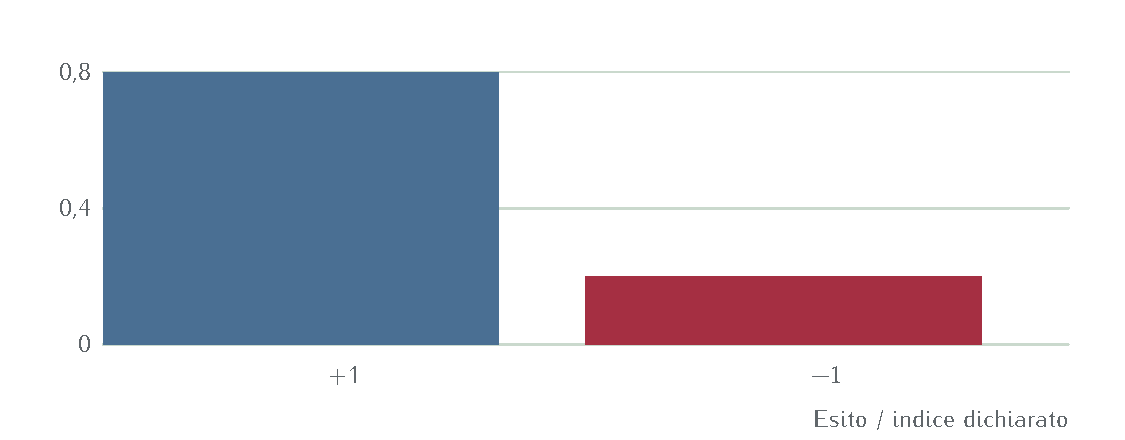
\includegraphics[width=\linewidth,height=94mm,keepaspectratio]{figure/f2bf4a4a978cd359e.pdf}\FigureCaption{2.26 \(\cdot\) esempio 1 \(\cdot\) Distribuzione degli esiti di \(Z\)}\end{FigureBlock}
\begin{FigureBlock}\begin{minipage}[t]{.485\linewidth}\centering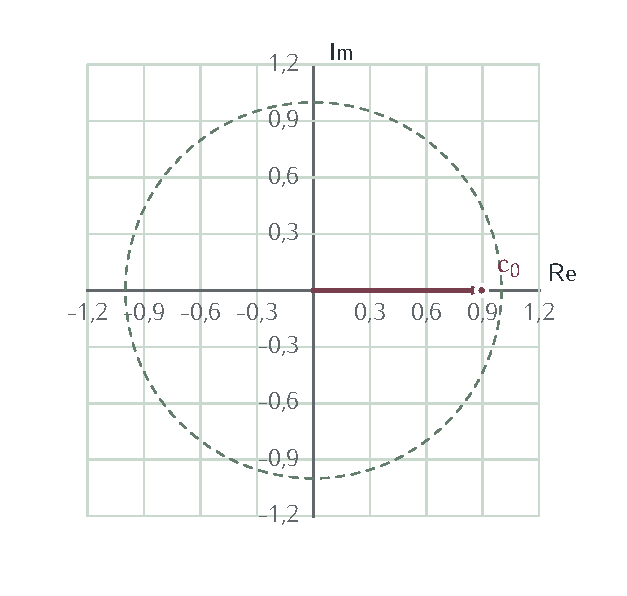
\includegraphics[width=\linewidth,height=63mm,keepaspectratio]{figure/f0364ff81b5e13f06.pdf}\par{\sffamily\footnotesize \(c_{0}\)\par}\end{minipage}\hfill\begin{minipage}[t]{.485\linewidth}\centering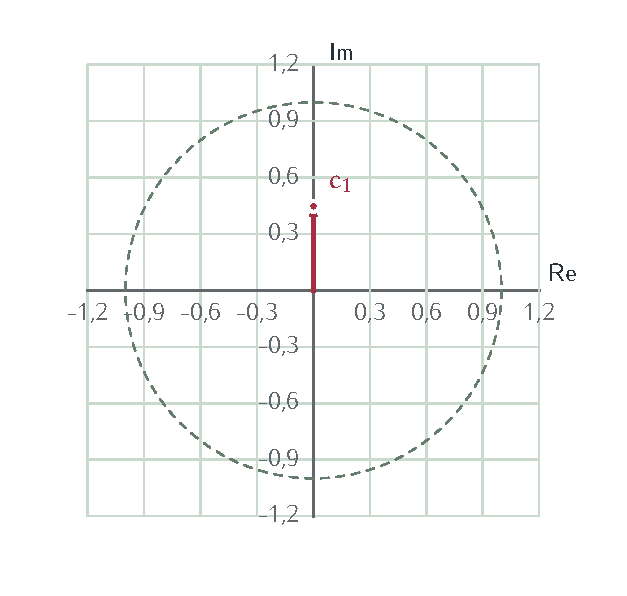
\includegraphics[width=\linewidth,height=63mm,keepaspectratio]{figure/f3671b82e02ed952e.pdf}\par{\sffamily\footnotesize \(c_{1}\)\par}\end{minipage}\FigureCaption{2.26 \(\cdot\) esempio 1 \(\cdot\) Componenti complesse}\end{FigureBlock}
\begin{FigureBlock}\centering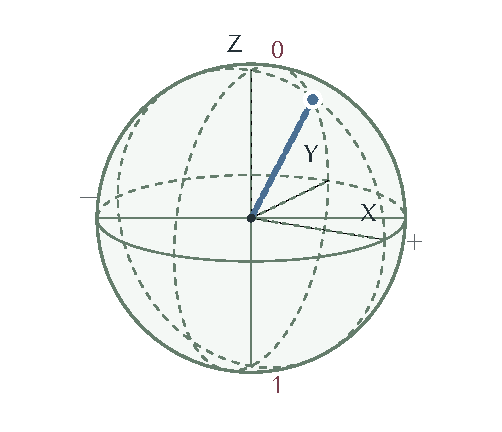
\includegraphics[width=\linewidth,height=94mm,keepaspectratio]{figure/fe3587a4d3c7cb4d0.pdf}\FigureCaption{2.26 \(\cdot\) esempio 1 \(\cdot\) Sfera di Bloch \(\cdot\) stato dell'esempio}\end{FigureBlock}

\phantomsection\label{c2-osservabili-example-1-step-1}
\BookHeading{01 Dichiarare autovalori e proiettori}

\MathBlock{0041003D005A003D005B005B0031002C0030005D002C005B0030002C22120031005D005D003D00412020}{A=Z=\begin{pmatrix}1&0\\0&- 1\end{pmatrix}=A{}^{\dagger} }
\MathBlock{005A007C003027E9003D002B007C003027E9003B0020005A007C003127E9003D2212007C003127E9}{Z|0\rangle =+|0\rangle ;\allowbreak \ Z|1\rangle =- |1\rangle }
\MathBlock{0050208A003D005B005B0031002C0030005D002C005B0030002C0030005D005D003B00200050208B003D005B005B0030002C0030005D002C005B0030002C0031005D005D}{P_{+}=\begin{pmatrix}1&0\\0&0\end{pmatrix};\allowbreak \ P_{-}=\begin{pmatrix}0&0\\0&1\end{pmatrix}}

Gli autovalori +1 e \(- 1\) sono i valori numerici osservati; 0 e 1 sono le etichette degli stati propri.\par


\phantomsection\label{c2-osservabili-example-1-step-2}
\BookHeading{02 Calcolare le probabilità}

\MathBlock{0061208A003D27E80030007C03C827E9003D0032002F221A0035003B00200070208A003D0034002F0035}{a_{+}=\langle 0|\psi \rangle =2/\sqrt{5};\allowbreak \ p_{+}=4/5}
\MathBlock{0061208B003D27E80031007C03C827E9003D0069002F221A0035003B00200070208B003D0031002F0035}{a_{-}=\langle 1|\psi \rangle =i/\sqrt{5};\allowbreak \ p_{-}=1/5}

I due moduli quadri sommano a uno.\par


\phantomsection\label{c2-osservabili-example-1-step-3}
\BookHeading{03 Calcolare media e secondo momento}

\MathBlock{27E8005A27E9003D003100B70034002F0035002B002822120031002900B70031002F0035003D0033002F0035}{\langle Z\rangle =1\cdot 4/5+(- 1)\cdot 1/5=3/5}
\MathBlock{005A00B2003D0049003B002027E8005A00B227E9003D003100B70034002F0035002B003100B70031002F0035003D0031}{Z^{2}=I;\allowbreak \ \langle Z^{2}\rangle =1\cdot 4/5+1\cdot 1/5=1}

Il secondo momento usa il quadrato degli esiti.\par


\phantomsection\label{c2-osservabili-example-1-step-4}
\BookHeading{04 Verificare con i prodotti matriciali}

\MathBlock{005A03C8003D00280032002C2212006900291D40002F221A0035}{Z\psi =(2,\allowbreak - i)^{T}/\sqrt{5}}
\MathBlock{27E803C8007C005A03C827E9003D005B003200B70032002B00282212006900290028221200690029005D002F0035003D00280034221200310029002F0035003D0033002F0035}{\langle \psi |Z\psi \rangle =[2\cdot 2+(- i)(- i)]/5=(4- 1)/5=3/5}
\MathBlock{0056006100720028005A0029003D0031221200280033002F0035002900B2003D00310036002F00320035003B002003C3005A003D0034002F0035}{\operatorname{Var}(Z)=1- (3/5)^{2}=16/25;\allowbreak \ \sigma Z=4/5}

La somma sullo spettro e il prodotto matriciale forniscono la stessa media.\par


\BookHeading{Interpretazione}

Il valore medio 3/5 non è un possibile esito singolo. La varianza 16/25 descrive la dispersione di misure su copie identiche.\par


\Needspace{.36\textheight}\phantomsection\label{c2-osservabili-example-2}
{\sffamily\small\color{Accent} ESEMPIO SVOLTO 2\par}
\BookHeading{Osservabile degenere: un solo esito}
Dati \(A=2I\) e \(\psi =(2,\allowbreak i)^{T}/\sqrt{5}\).\par


\BookHeading{Geometria e configurazione dell'esempio}
\begin{FigureBlock}\centering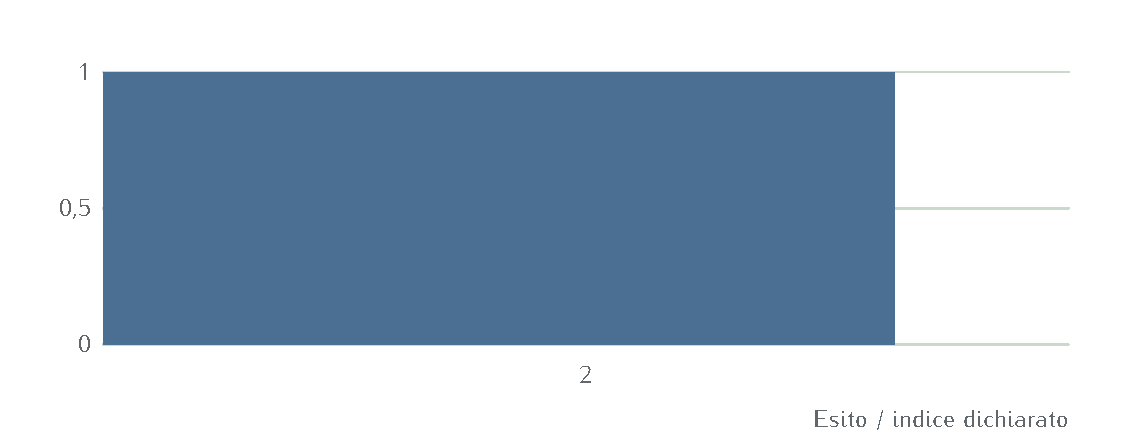
\includegraphics[width=\linewidth,height=94mm,keepaspectratio]{figure/fd73a96d36b463934.pdf}\FigureCaption{2.26 \(\cdot\) esempio 2 \(\cdot\) Unico esito dell'osservabile 2I}\end{FigureBlock}
\begin{FigureBlock}\begin{minipage}[t]{.485\linewidth}\centering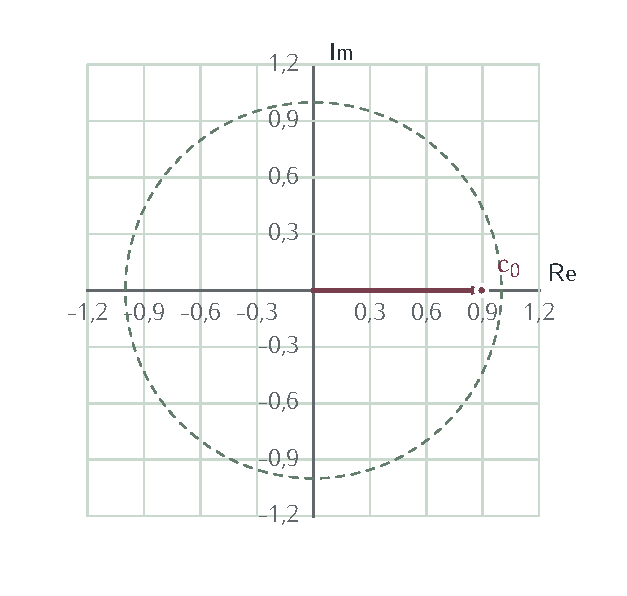
\includegraphics[width=\linewidth,height=63mm,keepaspectratio]{figure/f1843acf7fea75848.pdf}\par{\sffamily\footnotesize \(c_{0}\)\par}\end{minipage}\hfill\begin{minipage}[t]{.485\linewidth}\centering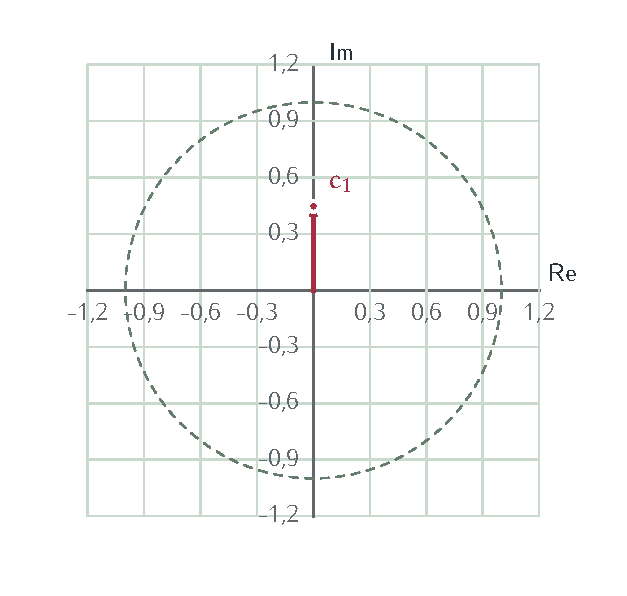
\includegraphics[width=\linewidth,height=63mm,keepaspectratio]{figure/fb8a5ede34fe12864.pdf}\par{\sffamily\footnotesize \(c_{1}\)\par}\end{minipage}\FigureCaption{2.26 \(\cdot\) esempio 2 \(\cdot\) Componenti complesse}\end{FigureBlock}
\begin{FigureBlock}\centering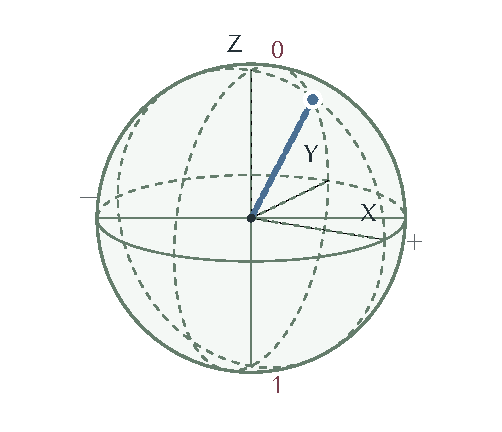
\includegraphics[width=\linewidth,height=94mm,keepaspectratio]{figure/fe3587a4d3c7cb4d0.pdf}\FigureCaption{2.26 \(\cdot\) esempio 2 \(\cdot\) Sfera di Bloch \(\cdot\) stato dell'esempio}\end{FigureBlock}

\phantomsection\label{c2-osservabili-example-2-step-1}
\BookHeading{01 Verificare l'operatore}

\MathBlock{0041003D00320049003D005B005B0032002C0030005D002C005B0030002C0032005D005D003D00412020003B002000640065007400280041221203BB00490029003D00280032221203BB002900B2}{A=2I=\begin{pmatrix}2&0\\0&2\end{pmatrix}=A{}^{\dagger} ;\allowbreak \ \det (A- \lambda I)=(2- \lambda )^{2}}

L'unico autovalore è 2 e il suo autospazio è tutto \(C^{2}\).\par


\phantomsection\label{c2-osservabili-example-2-step-2}
\BookHeading{02 Usare il proiettore sull'intero autospazio}

\MathBlock{00502082003D0049003B00200070002800320029003D27E803C8007C0049007C03C827E9003D00280034002B00310029002F0035003D0031}{P_{2}=I;\allowbreak \ p(2)=\langle \psi |I|\psi \rangle =(4+1)/5=1}
\MathBlock{0050208203C8003D03C8003B002003C82082003D03C8002F221A0031003D03C8}{P_{2}\psi =\psi ;\allowbreak \ \psi _{2}=\psi /\sqrt{1}=\psi }

La misura di questo operatore non distingue direzioni interne all'autospazio.\par


\phantomsection\label{c2-osservabili-example-2-step-3}
\BookHeading{03 Calcolare i momenti}

\MathBlock{27E8004127E9003D003200B70031003D0032003B0020004100B2003D00340049003B002027E8004100B227E9003D0034}{\langle A\rangle =2\cdot 1=2;\allowbreak \ A^{2}=4I;\allowbreak \ \langle A^{2}\rangle =4}
\MathBlock{005600610072002800410029003D00342212003200B2003D0030}{\operatorname{Var}(A)=4- 2^{2}=0}

L'esito è certo per qualunque stato normalizzato.\par


\phantomsection\label{c2-osservabili-example-2-step-4}
\BookHeading{04 Verificare direttamente sul ket}

\MathBlock{004103C8003D00280034002C0032006900291D40002F221A0035003D003203C8}{A\psi =(4{,}2i)^{T}/\sqrt{5}=2\psi }
\MathBlock{004100B203C8003D00280038002C0034006900291D40002F221A0035003D003403C8}{A^{2}\psi =(8{,}4i)^{T}/\sqrt{5}=4\psi }
\MathBlock{27E803C8007C004103C827E9003D003227E803C8007C03C827E9003D0032}{\langle \psi |A\psi \rangle =2\langle \psi |\psi \rangle =2}

Il calcolo matriciale conferma il singolo esito senza scegliere una base particolare dell'autospazio.\par


\BookHeading{Interpretazione}

La degenerazione richiede \(P_{2}=I\): l'esito vale sempre 2 e la preparazione resta \(\psi \). Una misura arbitraria delle due coordinate descriverebbe un esperimento diverso.\par


\Needspace{7\baselineskip}
\BookHeading{Il passaggio successivo}
La distribuzione di una singola osservabile è determinata. Per due misure successive servirà invece seguire lo stato condizionato in ciascun ramo e confrontare entrambi gli ordini.\par


\Needspace{.43\textheight}
\section{Due misure in successione}
\phantomsection\label{c2-incompatibilita}

{\sffamily\small\color{Ink!70} Riferimento alle slide: p. 433.\par}

{\sffamily\small\color{Ink!70} Laboratorio locale: \nolinkurl{index.html#capitolo-2/incompatibilita}\par}

\BookHeading{Definizioni e costruzione}
La prima misura seleziona uno stato condizionato. Per prevedere la seconda occorre usare quello stato in ciascun ramo e pesare il ramo con la sua probabilità.\par

Per una sequenza di misure si costruisce un ramo per ciascun primo esito. La seconda misura usa lo stato normalizzato di quel ramo; moltiplicando per la probabilità del primo esito si ottiene la distribuzione congiunta della sequenza. L'ordine delle misure può quindi modificare le statistiche.\par

Le dispersioni di due osservabili sulla preparazione iniziale si riferiscono invece a raccolte di copie identiche. La disuguaglianza di Robertson collega tali dispersioni al valore atteso del commutatore. Questa proprietà può essere presente anche in una descrizione ideale dell'apparato.\par


\MathBlock{00500028006A002C006B0029003D00500028006A002900500028006B007C006A0029002E}{P(j,\allowbreak k)=P(j)P(k|j).}

\BookHeading{Come leggere le figure}
Albero dei rami descritto da una distribuzione congiunta; esiti nulli non vengono normalizzati.\par


\Needspace{.36\textheight}\phantomsection\label{c2-incompatibilita-example-1}
{\sffamily\small\color{Accent} ESEMPIO SVOLTO 1\par}
\BookHeading{L'ordine modifica la distribuzione congiunta}
Dati \(\psi =(2,\allowbreak i)^{T}/\sqrt{5}\); confrontiamo \(X\to Z\) e \(Z\to X\) su copie preparate allo stesso modo.\par


\BookHeading{Geometria e configurazione dell'esempio}
\begin{FigureBlock}\centering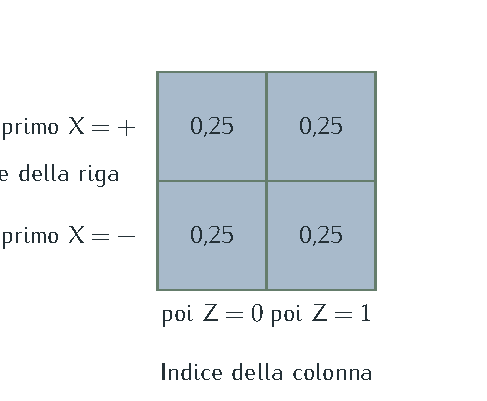
\includegraphics[width=\linewidth,height=94mm,keepaspectratio]{figure/f0221852baf1027e4.pdf}\FigureCaption{2.27 \(\cdot\) esempio 1 \(\cdot\) Ordine \(X\) poi \(Z\)}\end{FigureBlock}
\begin{FigureBlock}\centering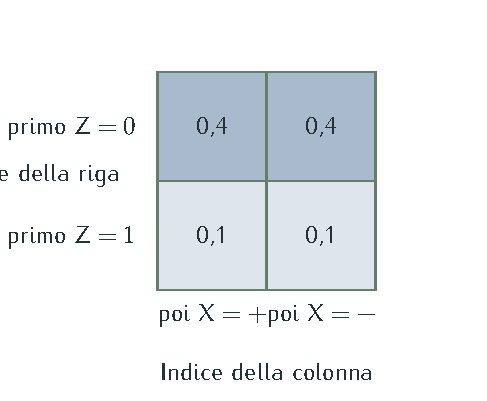
\includegraphics[width=\linewidth,height=94mm,keepaspectratio]{figure/f91339afc3ea21b8e.pdf}\FigureCaption{2.27 \(\cdot\) esempio 1 \(\cdot\) Ordine \(Z\) poi \(X\)}\end{FigureBlock}

\phantomsection\label{c2-incompatibilita-example-1-step-1}
\BookHeading{01 Dichiarare osservabili e basi}

\MathBlock{0058003D005B005B0030002C0031005D002C005B0031002C0030005D005D002C0020005A003D005B005B0031002C0030005D002C005B0030002C22120031005D005D002C00200059003D005B005B0030002C22120069005D002C005B0069002C0030005D005D}{X=\begin{pmatrix}0&1\\1&0\end{pmatrix},\allowbreak \ Z=\begin{pmatrix}1&0\\0&- 1\end{pmatrix},\allowbreak \ Y=\begin{pmatrix}0&- i\\i&0\end{pmatrix}}
\MathBlock{0058003A0020007C00B127E9003D00280031002C00B1003100291D40002F221A0032002C002000650073006900740069002000B10031}{X:\ |\pm \rangle =(1,\allowbreak \pm 1)^{T}/\sqrt{2},\allowbreak \ \text{esiti}\ \pm 1}
\MathBlock{005A003A0020007C003027E9002C007C003127E9002C0020006500730069007400690020002B0031002C22120031}{Z:\ |0\rangle ,\allowbreak |1\rangle ,\allowbreak \ \text{esiti}\ +1,\allowbreak - 1}

Le etichette 0,1 nelle tabelle identificano gli autostati di \(Z\); i segni \(+,\allowbreak - \) identificano quelli di \(X\).\par


\phantomsection\label{c2-incompatibilita-example-1-step-2}
\BookHeading{02 Calcolare la prima misura \(X\)}

\MathBlock{27E8002B007C03C827E9003D00280032002B00690029002F221A00310030003B002027E82212007C03C827E9003D00280032221200690029002F221A00310030}{\langle +|\psi \rangle =(2+i)/\sqrt{10};\allowbreak \ \langle - |\psi \rangle =(2- i)/\sqrt{10}}
\MathBlock{007000580028002B0029003D00700058002822120029003D00280034002B00310029002F00310030003D0031002F0032}{pX(+)=pX(- )=(4+1)/10=1/2}

Ogni ramo ha probabilità 1/2; lo stato condizionato è il corrispondente autostato \(X\), a meno di fase globale.\par


\phantomsection\label{c2-incompatibilita-example-1-step-3}
\BookHeading{03 Applicare \(Z\) nei due rami \(X\)}

\MathBlock{007C27E80030007C00B127E9007C00B2003D007C0031002F221A0032007C00B2003D0031002F0032}{|\langle 0|\pm \rangle |^{2}=|1/\sqrt{2}|^{2}=1/2}
\MathBlock{007C27E80031007C00B127E9007C00B2003D007C00B10031002F221A0032007C00B2003D0031002F0032}{|\langle 1|\pm \rangle |^{2}=|\pm 1/\sqrt{2}|^{2}=1/2}
\MathBlock{005000280058003D00B1002C005A003D006A0029003D00280031002F0032002900280031002F00320029003D0031002F0034}{P(X=\pm ,\allowbreak Z=j)=(1/2)(1/2)=1/4}

Le quattro probabilità congiunte derivano dalle probabilità del primo ramo moltiplicate per quelle condizionate.\par


\phantomsection\label{c2-incompatibilita-example-1-step-4}
\BookHeading{04 Invertire l'ordine: prima \(Z\)}

\MathBlock{27E80030007C03C827E9003D0032002F221A0035003B00200070005A002800300029003D0034002F0035}{\langle 0|\psi \rangle =2/\sqrt{5};\allowbreak \ pZ(0)=4/5}
\MathBlock{27E80031007C03C827E9003D0069002F221A0035003B00200070005A002800310029003D0031002F0035}{\langle 1|\psi \rangle =i/\sqrt{5};\allowbreak \ pZ(1)=1/5}

La prima misura ora prepara \(|0\rangle \) o \(|1\rangle \), con i pesi della distribuzione \(Z\) iniziale.\par


\phantomsection\label{c2-incompatibilita-example-1-step-5}
\BookHeading{05 Applicare \(X\) nei due rami \(Z\)}

\MathBlock{007C27E800B1007C003027E9007C00B2003D007C27E800B1007C003127E9007C00B2003D0031002F0032}{|\langle \pm |0\rangle |^{2}=|\langle \pm |1\rangle |^{2}=1/2}
\MathBlock{00500028005A003D0030002C0058003D00B10029003D0034002F00310030}{P(Z=0,\allowbreak X=\pm )=4/10}
\MathBlock{00500028005A003D0031002C0058003D00B10029003D0031002F00310030}{P(Z=1,\allowbreak X=\pm )=1/10}

Entrambi gli stati propri \(Z\) hanno coefficienti \(X\) di modulo \(1/\sqrt{2}\).\par


\phantomsection\label{c2-incompatibilita-example-1-step-6}
\BookHeading{06 Svolgere il commutatore}

\MathBlock{0058005A003D005B005B0030002C22120031005D002C005B0031002C0030005D005D003D221200690059}{XZ=\begin{pmatrix}0&- 1\\1&0\end{pmatrix}=- iY}
\MathBlock{005A0058003D005B005B0030002C0031005D002C005B22120031002C0030005D005D003D00690059}{ZX=\begin{pmatrix}0&1\\- 1&0\end{pmatrix}=iY}
\MathBlock{005B0058002C005A005D003D0058005A2212005A0058003D005B005B0030002C22120032005D002C005B0032002C0030005D005D003D2212003200690059}{[X,\allowbreak Z]=XZ- ZX=\begin{pmatrix}0&- 2\\2&0\end{pmatrix}=- 2iY}

Le due moltiplicazioni danno matrici opposte; il commutatore è un operatore non nullo, indipendentemente dalla preparazione.\par


\phantomsection\label{c2-incompatibilita-example-1-step-7}
\BookHeading{07 Calcolare i valori attesi sulla preparazione}

\MathBlock{005803C8003D00280069002C003200291D40002F221A0035003B002027E8005827E9003D0028003200692212003200690029002F0035003D0030}{X\psi =(i,\allowbreak 2)^{T}/\sqrt{5};\allowbreak \ \langle X\rangle =(2i- 2i)/5=0}
\MathBlock{005A03C8003D00280032002C2212006900291D40002F221A0035003B002027E8005A27E9003D00280034221200310029002F0035003D0030002C0036}{Z\psi =(2,\allowbreak - i)^{T}/\sqrt{5};\allowbreak \ \langle Z\rangle =(4- 1)/5=0{,}6}
\MathBlock{005903C8003D00280031002C0032006900291D40002F221A0035003B002027E8005927E9003D00280032002B00320029002F0035003D0030002C0038}{Y\psi =(1{,}2i)^{T}/\sqrt{5};\allowbreak \ \langle Y\rangle =(2+2)/5=0{,}8}

Questi prodotti interni si riferiscono a copie dello stesso stato iniziale, prima di qualsiasi misura.\par


\phantomsection\label{c2-incompatibilita-example-1-step-8}
\BookHeading{08 Ricavare varianze e limite di Robertson}

\MathBlock{005800B2003D005A00B2003D0049003B002027E8005800B227E9003D27E8005A00B227E9003D0031}{X^{2}=Z^{2}=I;\allowbreak \ \langle X^{2}\rangle =\langle Z^{2}\rangle =1}
\MathBlock{03C3005800B2003D00312212003000B2003D0031003B002003C3005A00B2003D0031221200280033002F0035002900B2003D00310036002F00320035}{\sigma X^{2}=1- 0^{2}=1;\allowbreak \ \sigma Z^{2}=1- (3/5)^{2}=16/25}
\MathBlock{03C3005803C3005A003D0034002F0035003D007C27E8005B0058002C005A005D27E9007C002F0032003D007C27E8005927E9007C}{\sigma X\sigma Z=4/5=|\langle [X,\allowbreak Z]\rangle |/2=|\langle Y\rangle |}

La disuguaglianza \(\sigma X\sigma Z\ge |\langle [X,\allowbreak Z]\rangle |/2\) è qui saturata. Essa riguarda dispersioni della preparazione, mentre le tabelle riguardano due misure sul medesimo sistema.\par


\BookHeading{Interpretazione}

\(X\to Z\) assegna 1/4 a ogni coppia; \(Z\to X\) assegna 2/5 alle coppie con primo risultato 0 e 1/10 alle altre. Lo stato condizionato del primo ramo spiega la differenza.\par


\Needspace{.36\textheight}\phantomsection\label{c2-incompatibilita-example-2}
{\sffamily\small\color{Accent} ESEMPIO SVOLTO 2\par}
\BookHeading{Statistiche uguali per una preparazione speciale}
Dati \(\psi =(1,\allowbreak i)^{T}/\sqrt{2}\); confrontiamo \(X\to Z\) e \(Z\to X\) su copie preparate allo stesso modo.\par


\BookHeading{Geometria e configurazione dell'esempio}
\begin{FigureBlock}\centering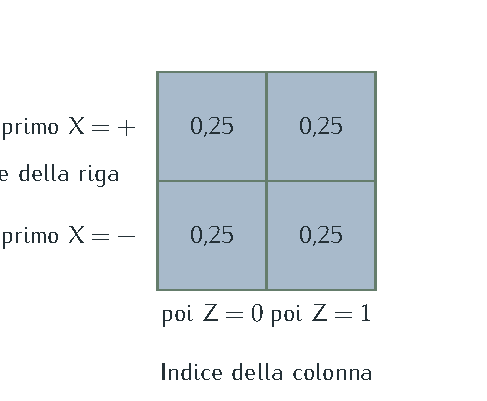
\includegraphics[width=\linewidth,height=94mm,keepaspectratio]{figure/f0221852baf1027e4.pdf}\FigureCaption{2.27 \(\cdot\) esempio 2 \(\cdot\) Ordine \(X\) poi \(Z\)}\end{FigureBlock}
\begin{FigureBlock}\centering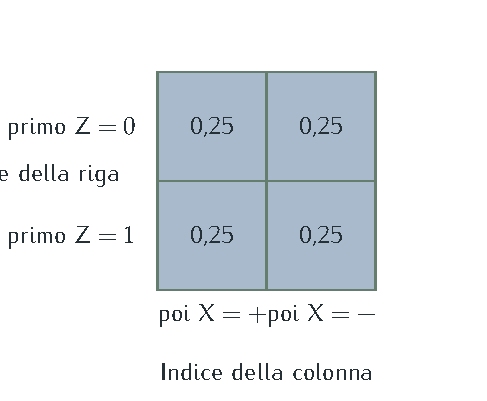
\includegraphics[width=\linewidth,height=94mm,keepaspectratio]{figure/f2aa00cf63a085a7b.pdf}\FigureCaption{2.27 \(\cdot\) esempio 2 \(\cdot\) Ordine \(Z\) poi \(X\)}\end{FigureBlock}

\phantomsection\label{c2-incompatibilita-example-2-step-1}
\BookHeading{01 Dichiarare osservabili e basi}

\MathBlock{0058003D005B005B0030002C0031005D002C005B0031002C0030005D005D002C0020005A003D005B005B0031002C0030005D002C005B0030002C22120031005D005D002C00200059003D005B005B0030002C22120069005D002C005B0069002C0030005D005D}{X=\begin{pmatrix}0&1\\1&0\end{pmatrix},\allowbreak \ Z=\begin{pmatrix}1&0\\0&- 1\end{pmatrix},\allowbreak \ Y=\begin{pmatrix}0&- i\\i&0\end{pmatrix}}
\MathBlock{0058003A0020007C00B127E9003D00280031002C00B1003100291D40002F221A0032002C002000650073006900740069002000B10031}{X:\ |\pm \rangle =(1,\allowbreak \pm 1)^{T}/\sqrt{2},\allowbreak \ \text{esiti}\ \pm 1}
\MathBlock{005A003A0020007C003027E9002C007C003127E9002C0020006500730069007400690020002B0031002C22120031}{Z:\ |0\rangle ,\allowbreak |1\rangle ,\allowbreak \ \text{esiti}\ +1,\allowbreak - 1}

Le etichette 0,1 nelle tabelle identificano gli autostati di \(Z\); i segni \(+,\allowbreak - \) identificano quelli di \(X\).\par


\phantomsection\label{c2-incompatibilita-example-2-step-2}
\BookHeading{02 Calcolare la prima misura \(X\)}

\MathBlock{27E8002B007C03C827E9003D00280031002B00690029002F221A0034003B002027E82212007C03C827E9003D00280031221200690029002F221A0034}{\langle +|\psi \rangle =(1+i)/\sqrt{4};\allowbreak \ \langle - |\psi \rangle =(1- i)/\sqrt{4}}
\MathBlock{007000580028002B0029003D00700058002822120029003D00280031002B00310029002F0034003D0031002F0032}{pX(+)=pX(- )=(1+1)/4=1/2}

Ogni ramo ha probabilità 1/2; lo stato condizionato è il corrispondente autostato \(X\), a meno di fase globale.\par


\phantomsection\label{c2-incompatibilita-example-2-step-3}
\BookHeading{03 Applicare \(Z\) nei due rami \(X\)}

\MathBlock{007C27E80030007C00B127E9007C00B2003D007C0031002F221A0032007C00B2003D0031002F0032}{|\langle 0|\pm \rangle |^{2}=|1/\sqrt{2}|^{2}=1/2}
\MathBlock{007C27E80031007C00B127E9007C00B2003D007C00B10031002F221A0032007C00B2003D0031002F0032}{|\langle 1|\pm \rangle |^{2}=|\pm 1/\sqrt{2}|^{2}=1/2}
\MathBlock{005000280058003D00B1002C005A003D006A0029003D00280031002F0032002900280031002F00320029003D0031002F0034}{P(X=\pm ,\allowbreak Z=j)=(1/2)(1/2)=1/4}

Le quattro probabilità congiunte derivano dalle probabilità del primo ramo moltiplicate per quelle condizionate.\par


\phantomsection\label{c2-incompatibilita-example-2-step-4}
\BookHeading{04 Invertire l'ordine: prima \(Z\)}

\MathBlock{27E80030007C03C827E9003D0031002F221A0032003B00200070005A002800300029003D0031002F0032}{\langle 0|\psi \rangle =1/\sqrt{2};\allowbreak \ pZ(0)=1/2}
\MathBlock{27E80031007C03C827E9003D0069002F221A0032003B00200070005A002800310029003D0031002F0032}{\langle 1|\psi \rangle =i/\sqrt{2};\allowbreak \ pZ(1)=1/2}

La prima misura ora prepara \(|0\rangle \) o \(|1\rangle \), con i pesi della distribuzione \(Z\) iniziale.\par


\phantomsection\label{c2-incompatibilita-example-2-step-5}
\BookHeading{05 Applicare \(X\) nei due rami \(Z\)}

\MathBlock{007C27E800B1007C003027E9007C00B2003D007C27E800B1007C003127E9007C00B2003D0031002F0032}{|\langle \pm |0\rangle |^{2}=|\langle \pm |1\rangle |^{2}=1/2}
\MathBlock{00500028005A003D0030002C0058003D00B10029003D0031002F0034}{P(Z=0,\allowbreak X=\pm )=1/4}
\MathBlock{00500028005A003D0031002C0058003D00B10029003D0031002F0034}{P(Z=1,\allowbreak X=\pm )=1/4}

Entrambi gli stati propri \(Z\) hanno coefficienti \(X\) di modulo \(1/\sqrt{2}\).\par


\phantomsection\label{c2-incompatibilita-example-2-step-6}
\BookHeading{06 Svolgere il commutatore}

\MathBlock{0058005A003D005B005B0030002C22120031005D002C005B0031002C0030005D005D003D221200690059}{XZ=\begin{pmatrix}0&- 1\\1&0\end{pmatrix}=- iY}
\MathBlock{005A0058003D005B005B0030002C0031005D002C005B22120031002C0030005D005D003D00690059}{ZX=\begin{pmatrix}0&1\\- 1&0\end{pmatrix}=iY}
\MathBlock{005B0058002C005A005D003D0058005A2212005A0058003D005B005B0030002C22120032005D002C005B0032002C0030005D005D003D2212003200690059}{[X,\allowbreak Z]=XZ- ZX=\begin{pmatrix}0&- 2\\2&0\end{pmatrix}=- 2iY}

Le due moltiplicazioni danno matrici opposte; il commutatore è un operatore non nullo, indipendentemente dalla preparazione.\par


\phantomsection\label{c2-incompatibilita-example-2-step-7}
\BookHeading{07 Calcolare i valori attesi sulla preparazione}

\MathBlock{005803C8003D00280069002C003100291D40002F221A0032003B002027E8005827E9003D0028003100692212003100690029002F0032003D0030}{X\psi =(i,\allowbreak 1)^{T}/\sqrt{2};\allowbreak \ \langle X\rangle =(1i- 1i)/2=0}
\MathBlock{005A03C8003D00280031002C2212006900291D40002F221A0032003B002027E8005A27E9003D00280031221200310029002F0032003D0030}{Z\psi =(1,\allowbreak - i)^{T}/\sqrt{2};\allowbreak \ \langle Z\rangle =(1- 1)/2=0}
\MathBlock{005903C8003D00280031002C0031006900291D40002F221A0032003B002027E8005927E9003D00280031002B00310029002F0032003D0031}{Y\psi =(1{,}1i)^{T}/\sqrt{2};\allowbreak \ \langle Y\rangle =(1+1)/2=1}

Questi prodotti interni si riferiscono a copie dello stesso stato iniziale, prima di qualsiasi misura.\par


\phantomsection\label{c2-incompatibilita-example-2-step-8}
\BookHeading{08 Ricavare varianze e limite di Robertson}

\MathBlock{005800B2003D005A00B2003D0049003B002027E8005800B227E9003D27E8005A00B227E9003D0031}{X^{2}=Z^{2}=I;\allowbreak \ \langle X^{2}\rangle =\langle Z^{2}\rangle =1}
\MathBlock{03C3005800B2003D00312212003000B2003D0031003B002003C3005A00B2003D0031221200280030002F0032002900B2003D0034002F0034}{\sigma X^{2}=1- 0^{2}=1;\allowbreak \ \sigma Z^{2}=1- (0/2)^{2}=4/4}
\MathBlock{03C3005803C3005A003D0032002F0032003D007C27E8005B0058002C005A005D27E9007C002F0032003D007C27E8005927E9007C}{\sigma X\sigma Z=2/2=|\langle [X,\allowbreak Z]\rangle |/2=|\langle Y\rangle |}

La disuguaglianza \(\sigma X\sigma Z\ge |\langle [X,\allowbreak Z]\rangle |/2\) è qui saturata. Essa riguarda dispersioni della preparazione, mentre le tabelle riguardano due misure sul medesimo sistema.\par


\BookHeading{Interpretazione}

Per \(\psi =(1,\allowbreak i)/\sqrt{2}\) entrambe le tabelle sono uniformi. Questa uguaglianza su una sola preparazione non implica commutatività: il calcolo \(XZ- ZX=- 2iY\) resta non nullo.\par


\Needspace{7\baselineskip}
\BookHeading{Il passaggio successivo}
L'ordine delle misure e le dispersioni su copie hanno ruoli distinti. Riuniremo i calcoli in un esperimento con un'osservabile complessa esplicitamente dichiarata.\par


\Needspace{.43\textheight}
\section{Un esperimento completo}
\phantomsection\label{c2-esperimento}

{\sffamily\small\color{Ink!70} Riferimento alle slide: p. 488.\par}

{\sffamily\small\color{Ink!70} Laboratorio locale: \nolinkurl{index.html#capitolo-2/esperimento}\par}

\BookHeading{Definizioni e costruzione}
Riuniamo normalizzazione, base propria, proiezioni, media e varianza in un unico calcolo. Ogni risultato viene controllato attraverso una seconda identità.\par

Il calcolo completo inizia controllando i dati: lo stato deve essere normalizzato e l'operatore deve essere hermitiano. Si determinano poi gli autovalori, si risolvono i sistemi per gli autovettori e si controllano normalizzazione e ortogonalità.\par

I prodotti interni forniscono ampiezze e probabilità. Media e varianza vengono calcolate attraverso lo spettro e confrontate con le espressioni matriciali. Infine il proiettore del ramo scelto permette di ricavare lo stato successivo alla misura. Le frazioni esatte vengono mantenute accanto ai valori decimali.\par


\MathBlock{0041003D00412020003B00200041003D03A303BB2C7C00502C7C003B002000702C7C003D27E803C8007C00502C7C007C03C827E9002E}{A=A{}^{\dagger} ;\allowbreak \ A=\sum \lambda _{j}P_{j};\allowbreak \ p_{j}=\langle \psi |P_{j}|\psi \rangle .}

\BookHeading{Come leggere le figure}
Autospazi di \(C^{2}\) e distribuzione degli autovalori; le ampiezze conservano le fasi.\par


\Needspace{.36\textheight}\phantomsection\label{c2-esperimento-example-1}
{\sffamily\small\color{Accent} ESEMPIO SVOLTO 1\par}
\BookHeading{Misura di un'osservabile complessa}
Dati \(A=\)\(\begin{pmatrix}1&1- i\\1+i&0\end{pmatrix}\), \(\psi =(2,\allowbreak i)^{T}/\sqrt{5}\); gli esiti della misura saranno gli autovalori di \(A\).\par


\BookHeading{Geometria e configurazione dell'esempio}
\begin{FigureBlock}\centering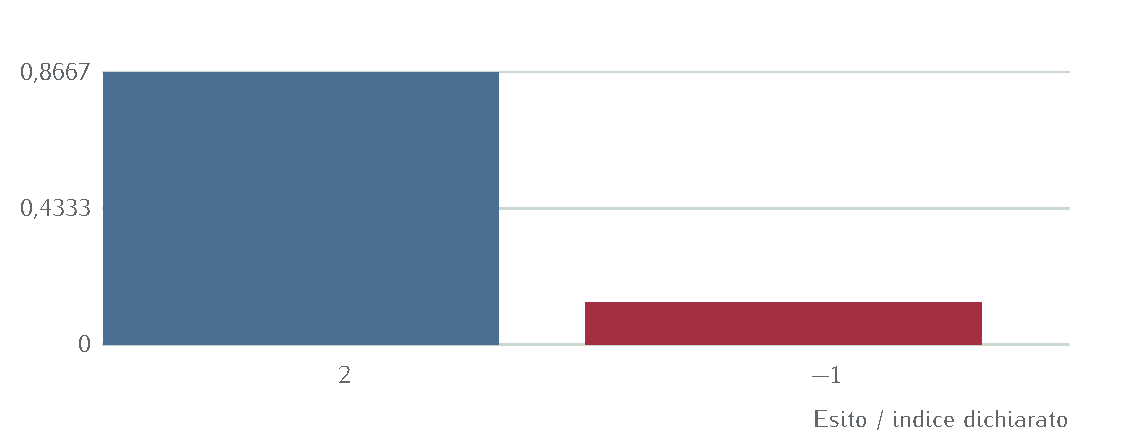
\includegraphics[width=\linewidth,height=94mm,keepaspectratio]{figure/fa4a9484d1ecf7c24.pdf}\FigureCaption{2.28 \(\cdot\) esempio 1 \(\cdot\) Distribuzione degli autovalori}\end{FigureBlock}
\begin{FigureBlock}\begin{minipage}[t]{.485\linewidth}\centering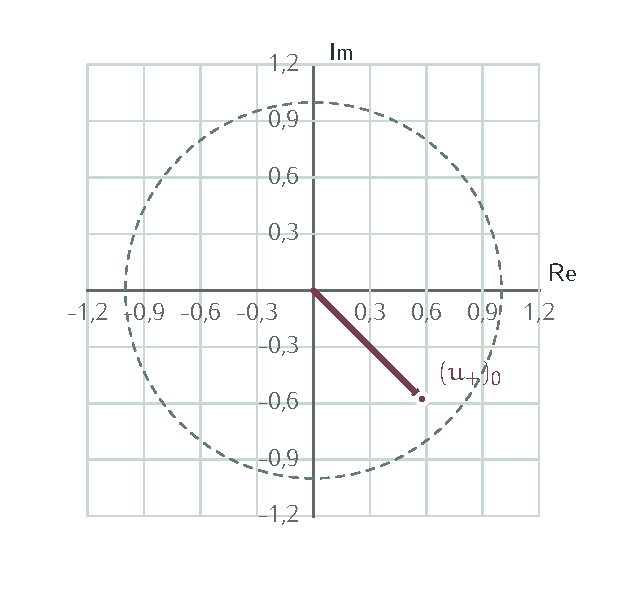
\includegraphics[width=\linewidth,height=63mm,keepaspectratio]{figure/f3400ae11e2a3a099.pdf}\par{\sffamily\footnotesize \((u_{+})_{0}\)\par}\end{minipage}\hfill\begin{minipage}[t]{.485\linewidth}\centering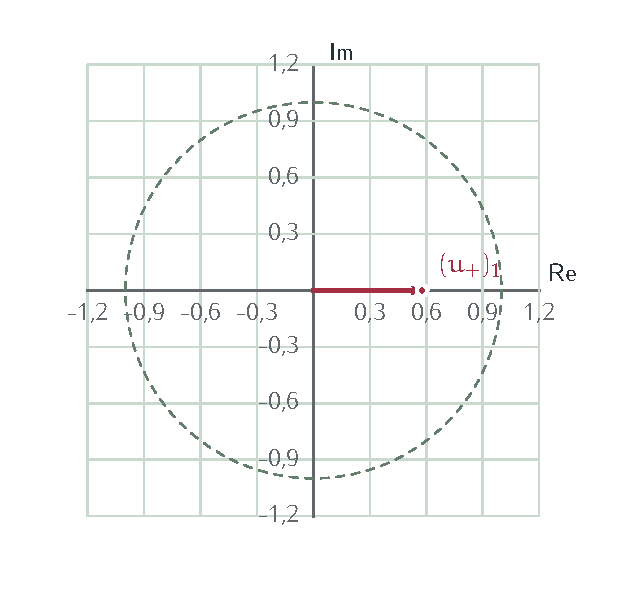
\includegraphics[width=\linewidth,height=63mm,keepaspectratio]{figure/ffad125b90e0a03ef.pdf}\par{\sffamily\footnotesize \((u_{+})_{1}\)\par}\end{minipage}\FigureCaption{2.28 \(\cdot\) esempio 1 \(\cdot\) Autovettori della base di misura}\end{FigureBlock}
\begin{FigureBlock}\begin{minipage}[t]{.485\linewidth}\centering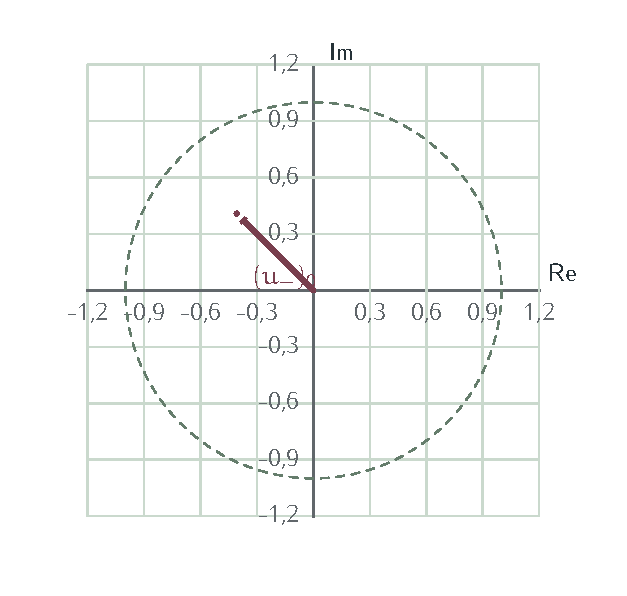
\includegraphics[width=\linewidth,height=63mm,keepaspectratio]{figure/f7524f6dd53e552f1.pdf}\par{\sffamily\footnotesize \((u_{-})_{0}\)\par}\end{minipage}\hfill\begin{minipage}[t]{.485\linewidth}\centering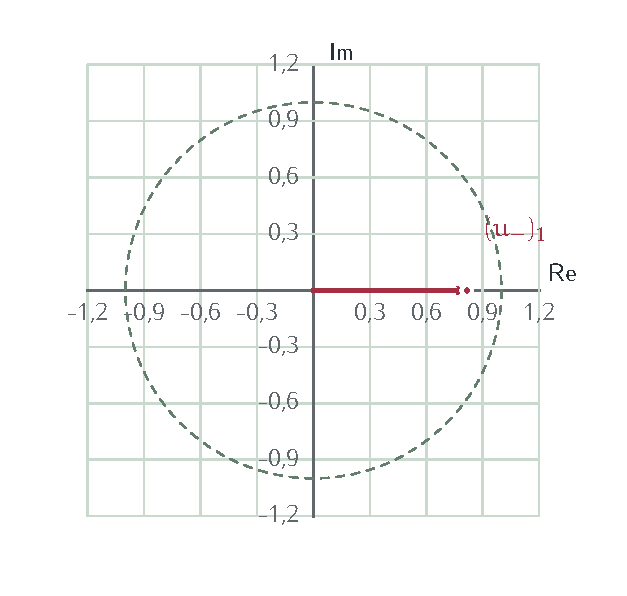
\includegraphics[width=\linewidth,height=63mm,keepaspectratio]{figure/f241a93486f2a3068.pdf}\par{\sffamily\footnotesize \((u_{-})_{1}\)\par}\end{minipage}\FigureCaption{2.28 \(\cdot\) esempio 1 \(\cdot\) Autovettori della base di misura}\end{FigureBlock}
\begin{FigureBlock}\begin{minipage}[t]{.485\linewidth}\centering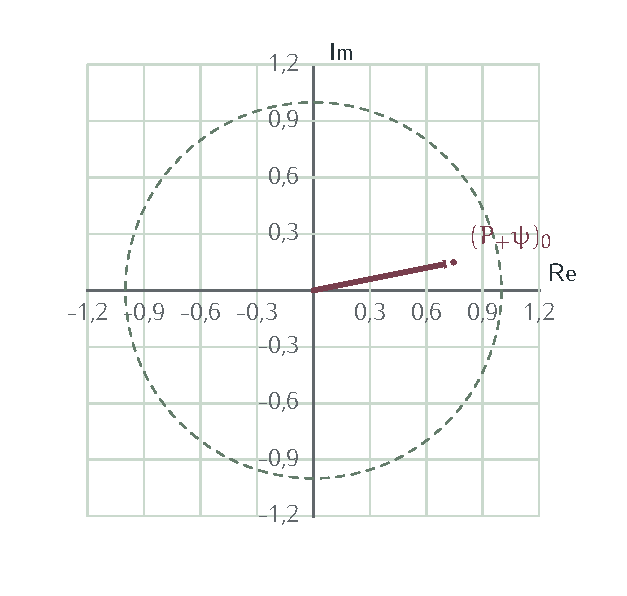
\includegraphics[width=\linewidth,height=63mm,keepaspectratio]{figure/f6b1af56db923ad3b.pdf}\par{\sffamily\footnotesize \((P_{+}\psi )_{0}\)\par}\end{minipage}\hfill\begin{minipage}[t]{.485\linewidth}\centering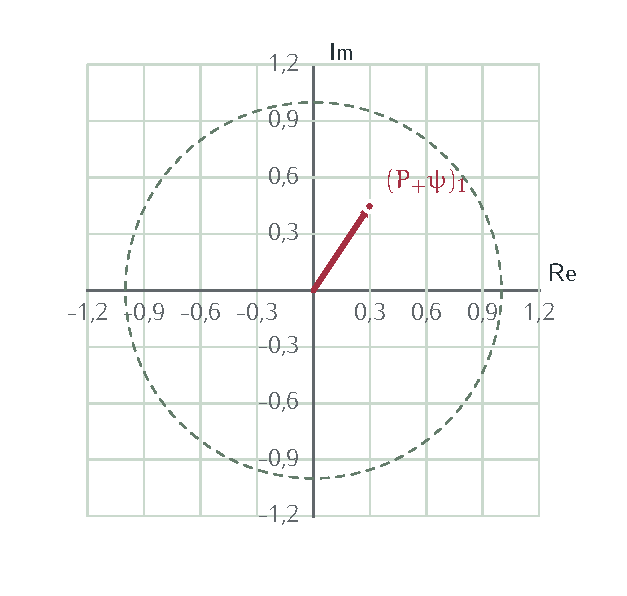
\includegraphics[width=\linewidth,height=63mm,keepaspectratio]{figure/f8239656e13032b16.pdf}\par{\sffamily\footnotesize \((P_{+}\psi )_{1}\)\par}\end{minipage}\FigureCaption{2.28 \(\cdot\) esempio 1 \(\cdot\) Proiezioni prima della rinormalizzazione}\end{FigureBlock}
\begin{FigureBlock}\begin{minipage}[t]{.485\linewidth}\centering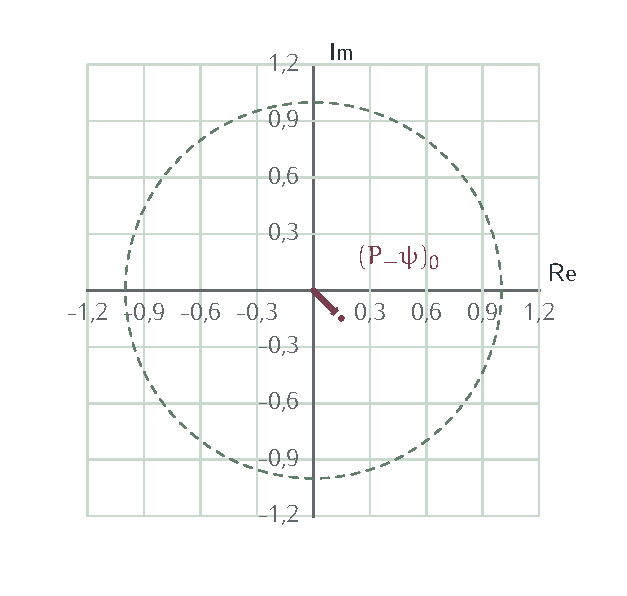
\includegraphics[width=\linewidth,height=63mm,keepaspectratio]{figure/ff501c8bb815bffb4.pdf}\par{\sffamily\footnotesize \((P_{-}\psi )_{0}\)\par}\end{minipage}\hfill\begin{minipage}[t]{.485\linewidth}\centering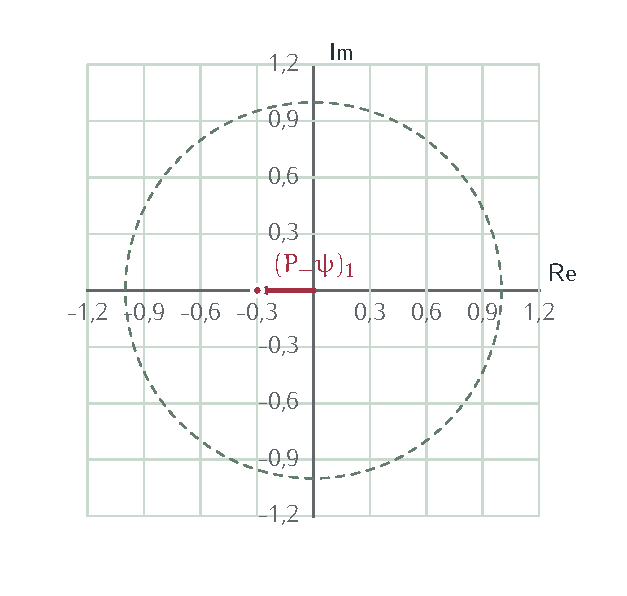
\includegraphics[width=\linewidth,height=63mm,keepaspectratio]{figure/f5650b7abba469e3d.pdf}\par{\sffamily\footnotesize \((P_{-}\psi )_{1}\)\par}\end{minipage}\FigureCaption{2.28 \(\cdot\) esempio 1 \(\cdot\) Proiezioni prima della rinormalizzazione}\end{FigureBlock}

\phantomsection\label{c2-esperimento-example-1-step-1}
\BookHeading{01 Controllare tutti i dati}

\MathBlock{0041003D005B005B0031002C003122120069005D002C005B0031002B0069002C0030005D005D}{A=\begin{pmatrix}1&1- i\\1+i&0\end{pmatrix}}
\MathBlock{00412020003D005B005B0031002C00280031002B00690029002A005D002C005B00280031221200690029002A002C0030005D005D003D0041}{A{}^{\dagger} =\begin{pmatrix}1&(1+i){}^{*}\\(1- i){}^{*}&0\end{pmatrix}=A}
\MathBlock{03C8003D00280032002C006900291D40002F221A0035003B0020201603C8201600B2003D00280034002B00310029002F0035003D0031}{\psi =(2,\allowbreak i)^{T}/\sqrt{5};\allowbreak \ \Vert \psi \Vert ^{2}=(4+1)/5=1}

La diagonale di \(A\) è reale e i termini fuori diagonale sono coniugati: \(A\) è un'osservabile hermitiana.\par


\phantomsection\label{c2-esperimento-example-1-step-2}
\BookHeading{02 Determinare gli autovalori}

\MathBlock{00640065007400280041221203BB00490029003D00280031221203BB00290028221203BB002922120028003122120069002900280031002B00690029}{\det (A- \lambda I)=(1- \lambda )(- \lambda )- (1- i)(1+i)}
\MathBlock{003D03BB00B2221203BB22120032003D002803BB221200320029002803BB002B00310029003D0030}{=\lambda ^{2}- \lambda - 2=(\lambda - 2)(\lambda +1)=0}
\MathBlock{03BB208A003D0032003B002003BB208B003D22120031}{\lambda _{+}=2;\allowbreak \ \lambda _{-}=- 1}

Il prodotto dei termini complessi vale \((1- i)(1+i)=2\).\par


\phantomsection\label{c2-esperimento-example-1-step-3}
\BookHeading{03 Risolvere il primo autovettore}

\MathBlock{03BB003D0032003A002022120078002B002800312212006900290079003D0030003B00200073006300650067006C00690061006D006F00200079003D0031002021D200200078003D003122120069}{\lambda =2:\ - x+(1- i)y=0;\allowbreak \ \text{scegliamo}\ y=1\ \Rightarrow \ x=1- i}
\MathBlock{00280031002B006900290028003122120069002922120032003D0030}{(1+i)(1- i)- 2=0}
\MathBlock{20160028003122120069002C00310029201600B2003D0032002B0031003D0033003B00200075208A003D0028003122120069002C003100291D40002F221A0033}{\Vert (1- i,\allowbreak 1)\Vert ^{2}=2+1=3;\allowbreak \ u_{+}=(1- i,\allowbreak 1)^{T}/\sqrt{3}}

Il candidato soddisfa entrambe le equazioni; dividere per \(\sqrt{3}\) lo normalizza.\par


\phantomsection\label{c2-esperimento-example-1-step-4}
\BookHeading{04 Risolvere il secondo autovettore}

\MathBlock{03BB003D22120031003A002000320078002B002800312212006900290079003D0030003B00200073006300650067006C00690061006D006F00200079003D0032002021D200200078003D22120031002B0069}{\lambda =- 1:\ 2x+(1- i)y=0;\allowbreak \ \text{scegliamo}\ y=2\ \Rightarrow \ x=- 1+i}
\MathBlock{00280031002B00690029002822120031002B00690029002B0032003D0030}{(1+i)(- 1+i)+2=0}
\MathBlock{2016002822120031002B0069002C00320029201600B2003D0032002B0034003D0036003B00200075208B003D002822120031002B0069002C003200291D40002F221A0036}{\Vert (- 1+i,\allowbreak 2)\Vert ^{2}=2+4=6;\allowbreak \ u_{-}=(- 1+i,\allowbreak 2)^{T}/\sqrt{6}}

Gli autovalori distinti individuano due autospazi di dimensione uno.\par


\phantomsection\label{c2-esperimento-example-1-step-5}
\BookHeading{05 Verificare l'ortogonalità}

\MathBlock{27E80075208A007C0075208B27E9003D005B00280031002B00690029002822120031002B00690029002B0032005D002F221A00310038003D002822120032002B00320029002F221A00310038003D0030}{\langle u_{+}|u_{-}\rangle =[(1+i)(- 1+i)+2]/\sqrt{18}=(- 2+2)/\sqrt{18}=0}

I due vettori normalizzati costituiscono una base ortonormale di \(C^{2}\).\par


\phantomsection\label{c2-esperimento-example-1-step-6}
\BookHeading{06 Calcolare le ampiezze esatte}

\MathBlock{0061208A003D005B00280031002B0069002900B70032002B0069005D002F221A00310035003D00280032002B003300690029002F221A00310035}{a_{+}=[(1+i)\cdot 2+i]/\sqrt{15}=(2+3i)/\sqrt{15}}
\MathBlock{0061208B003D005B00282212003122120069002900B70032002B00320069005D002F221A00330030003D22120032002F221A00330030}{a_{-}=[(- 1- i)\cdot 2+2i]/\sqrt{30}=- 2/\sqrt{30}}

I bra degli autovettori coniugano la prima componente prima del prodotto.\par


\phantomsection\label{c2-esperimento-example-1-step-7}
\BookHeading{07 Calcolare e sommare i moduli quadri}

\MathBlock{0070208A003D0028003200B2002B003300B20029002F00310035003D00310033002F00310035003B00200070208B003D0034002F00330030003D0032002F00310035}{p_{+}=(2^{2}+3^{2})/15=13/15;\allowbreak \ p_{-}=4/30=2/15}
\MathBlock{0070208A002B0070208B003D0031}{p_{+}+p_{-}=1}

Le due probabilità coprono tutti gli esiti della misura.\par


\phantomsection\label{c2-esperimento-example-1-step-8}
\BookHeading{08 Proiettare nel ramo +}

\MathBlock{0050002B03C8003D0075002B0061002B224800280030002C00370034003500340020002B00200030002C00310034003900310069003B00200030002C00320039003800310020002B00200030002C0034003400370032006900291D40}{P+\psi =u+a+\approx (0{,}7454\ +\ 0{,}1491i;\allowbreak \ 0{,}2981\ +\ 0{,}4472i)^{T}}
\MathBlock{03C8002B003D0050002B03C8002F221A0070002B224800280030002C00380030003000360020002B00200030002C00310036003000310069003B00200030002C00330032003000330020002B00200030002C0034003800300034006900291D40}{\psi +=P+\psi /\sqrt{p}+\approx (0{,}8006\ +\ 0{,}1601i;\allowbreak \ 0{,}3203\ +\ 0{,}4804i)^{T}}

Il ramo è possibile perché il suo peso è positivo. Lo stato condizionato ha norma uno e appartiene al relativo autospazio.\par


\phantomsection\label{c2-esperimento-example-1-step-9}
\BookHeading{09 Proiettare nel ramo \(- \)}

\MathBlock{0050221203C8003D0075221200612212224800280030002C00310034003900310020221200200030002C00310034003900310069003B0020002D0030002C003200390038003100291D40}{P- \psi =u- a- \approx (0{,}1491\ - \ 0{,}1491i;\allowbreak \ -0{,}2981)^{T}}
\MathBlock{03C82212003D0050221203C8002F221A00702212224800280030002C00340030003800320020221200200030002C00340030003800320069003B0020002D0030002C003800310036003500291D40}{\psi - =P- \psi /\sqrt{p}- \approx (0{,}4082\ - \ 0{,}4082i;\allowbreak \ -0{,}8165)^{T}}

Il ramo è possibile perché il suo peso è positivo. Lo stato condizionato ha norma uno e appartiene al relativo autospazio.\par


\phantomsection\label{c2-esperimento-example-1-step-10}
\BookHeading{10 Calcolare i momenti dallo spettro}

\MathBlock{27E8004127E9003D003200B700310033002F0031003522120032002F00310035003D0038002F0035}{\langle A\rangle =2\cdot 13/15- 2/15=8/5}
\MathBlock{27E8004100B227E9003D003400B700310033002F00310035002B0032002F00310035003D00310038002F0035}{\langle A^{2}\rangle =4\cdot 13/15+2/15=18/5}
\MathBlock{005600610072002800410029003D00310038002F0035221200280038002F0035002900B2003D00320036002F00320035}{\operatorname{Var}(A)=18/5- (8/5)^{2}=26/25}

Si pesano prima gli esiti, poi i loro quadrati; la varianza sottrae il quadrato della media.\par


\phantomsection\label{c2-esperimento-example-1-step-11}
\BookHeading{11 Verifica \(A\psi \), riga 1}

\MathBlock{00280031002900B700280030002C003800390034003400290020002B0020002800310020221200200069002900B700280030002C00340034003700320069002922480031002C00330034003100360020002B00200030002C00340034003700320069}{(1)\cdot (0{,}8944)\ +\ (1\ - \ i)\cdot (0{,}4472i)\approx 1{,}3416\ +\ 0{,}4472i}

Ogni riga usa direttamente la preparazione normalizzata.\par


\phantomsection\label{c2-esperimento-example-1-step-12}
\BookHeading{12 Verifica \(A\psi \), riga 2}

\MathBlock{002800310020002B00200069002900B700280030002C003800390034003400290020002B002000280030002900B700280030002C00340034003700320069002922480030002C00380039003400340020002B00200030002C00380039003400340069}{(1\ +\ i)\cdot (0{,}8944)\ +\ (0)\cdot (0{,}4472i)\approx 0{,}8944\ +\ 0{,}8944i}

Ogni riga usa direttamente la preparazione normalizzata.\par


\phantomsection\label{c2-esperimento-example-1-step-13}
\BookHeading{13 Verifica \(A^{2}\psi \), riga 1}

\MathBlock{00280031002900B700280031002C00330034003100360020002B00200030002C0034003400370032006900290020002B0020002800310020221200200069002900B700280030002C00380039003400340020002B00200030002C00380039003400340069002922480033002C00310033003000350020002B00200030002C00340034003700320069}{(1)\cdot (1{,}3416\ +\ 0{,}4472i)\ +\ (1\ - \ i)\cdot (0{,}8944\ +\ 0{,}8944i)\approx 3{,}1305\ +\ 0{,}4472i}

La seconda applicazione usa l'uscita \(A\psi \) appena ottenuta.\par


\phantomsection\label{c2-esperimento-example-1-step-14}
\BookHeading{14 Verifica \(A^{2}\psi \), riga 2}

\MathBlock{002800310020002B00200069002900B700280031002C00330034003100360020002B00200030002C0034003400370032006900290020002B002000280030002900B700280030002C00380039003400340020002B00200030002C00380039003400340069002922480030002C00380039003400340020002B00200031002C00370038003800390069}{(1\ +\ i)\cdot (1{,}3416\ +\ 0{,}4472i)\ +\ (0)\cdot (0{,}8944\ +\ 0{,}8944i)\approx 0{,}8944\ +\ 1{,}7889i}

La seconda applicazione usa l'uscita \(A\psi \) appena ottenuta.\par


\phantomsection\label{c2-esperimento-example-1-step-15}
\BookHeading{15 Confrontare i momenti matriciali}

\MathBlock{27E803C8007C004103C827E9003D00280030002C0038003900340034002900B700280031002C00330034003100360020002B00200030002C0034003400370032006900290020002B00200028002D0030002C00340034003700320069002900B700280030002C00380039003400340020002B00200030002C00380039003400340069002922480031002C0036}{\langle \psi |A\psi \rangle =(0{,}8944)\cdot (1{,}3416\ +\ 0{,}4472i)\ +\ (-0{,}4472i)\cdot (0{,}8944\ +\ 0{,}8944i)\approx 1{,}6}
\MathBlock{27E803C8007C004100B203C827E9003D00280030002C0038003900340034002900B700280033002C00310033003000350020002B00200030002C0034003400370032006900290020002B00200028002D0030002C00340034003700320069002900B700280030002C00380039003400340020002B00200031002C00370038003800390069002922480033002C0036}{\langle \psi |A^{2}\psi \rangle =(0{,}8944)\cdot (3{,}1305\ +\ 0{,}4472i)\ +\ (-0{,}4472i)\cdot (0{,}8944\ +\ 1{,}7889i)\approx 3{,}6}
\MathBlock{00560061007200280041002922480031002C00300034}{\operatorname{Var}(A)\approx 1{,}04}

I prodotti matriciali confermano le frazioni ricavate indipendentemente dallo spettro.\par


\BookHeading{Interpretazione}

La preparazione produce probabilità (13/15,2/15), media 8/5 e varianza 26/25. Due calcoli indipendenti, spettrale e matriciale, concordano.\par


\Needspace{.36\textheight}\phantomsection\label{c2-esperimento-example-2}
{\sffamily\small\color{Accent} ESEMPIO SVOLTO 2\par}
\BookHeading{Stessa osservabile, preparazione equatoriale}
Dati \(A=\)\(\begin{pmatrix}1&1- i\\1+i&0\end{pmatrix}\), \(\psi =(1,\allowbreak i)^{T}/\sqrt{2}\); gli esiti della misura saranno gli autovalori di \(A\).\par


\BookHeading{Geometria e configurazione dell'esempio}
\begin{FigureBlock}\centering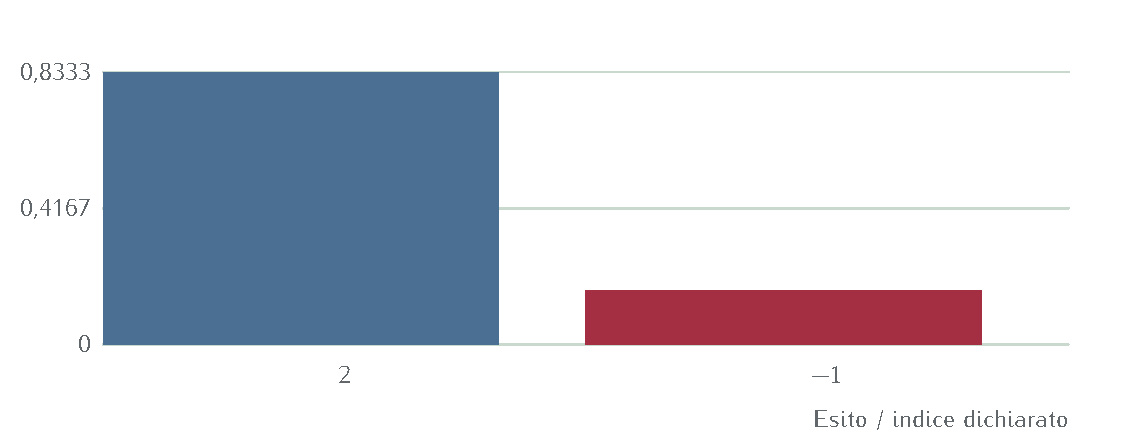
\includegraphics[width=\linewidth,height=94mm,keepaspectratio]{figure/f59985c31da7fb0c1.pdf}\FigureCaption{2.28 \(\cdot\) esempio 2 \(\cdot\) Distribuzione degli autovalori}\end{FigureBlock}
\begin{FigureBlock}\begin{minipage}[t]{.485\linewidth}\centering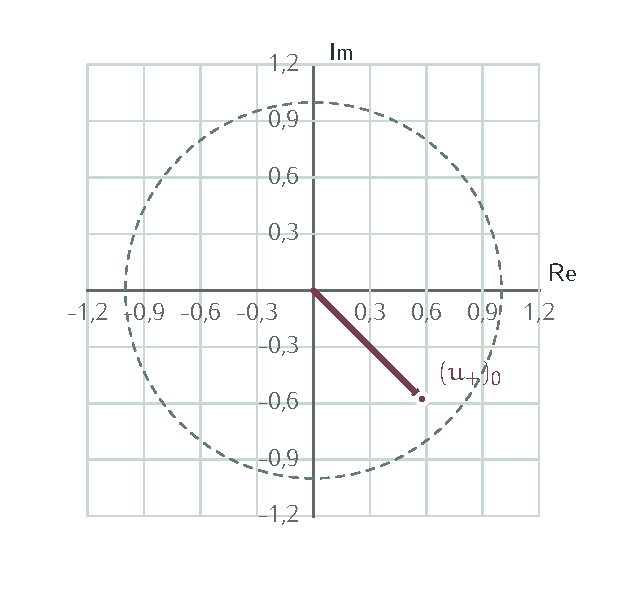
\includegraphics[width=\linewidth,height=63mm,keepaspectratio]{figure/fc555621e523c11d3.pdf}\par{\sffamily\footnotesize \((u_{+})_{0}\)\par}\end{minipage}\hfill\begin{minipage}[t]{.485\linewidth}\centering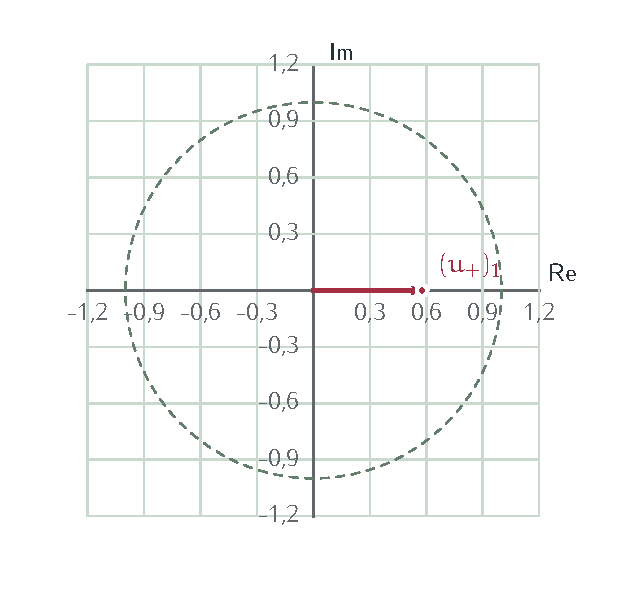
\includegraphics[width=\linewidth,height=63mm,keepaspectratio]{figure/f488e060c402c4135.pdf}\par{\sffamily\footnotesize \((u_{+})_{1}\)\par}\end{minipage}\FigureCaption{2.28 \(\cdot\) esempio 2 \(\cdot\) Autovettori della base di misura}\end{FigureBlock}
\begin{FigureBlock}\begin{minipage}[t]{.485\linewidth}\centering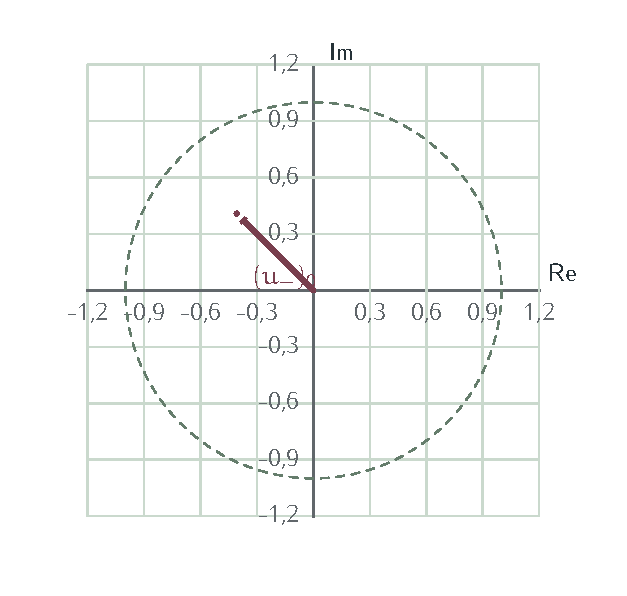
\includegraphics[width=\linewidth,height=63mm,keepaspectratio]{figure/f5b4308aa03b5d9cf.pdf}\par{\sffamily\footnotesize \((u_{-})_{0}\)\par}\end{minipage}\hfill\begin{minipage}[t]{.485\linewidth}\centering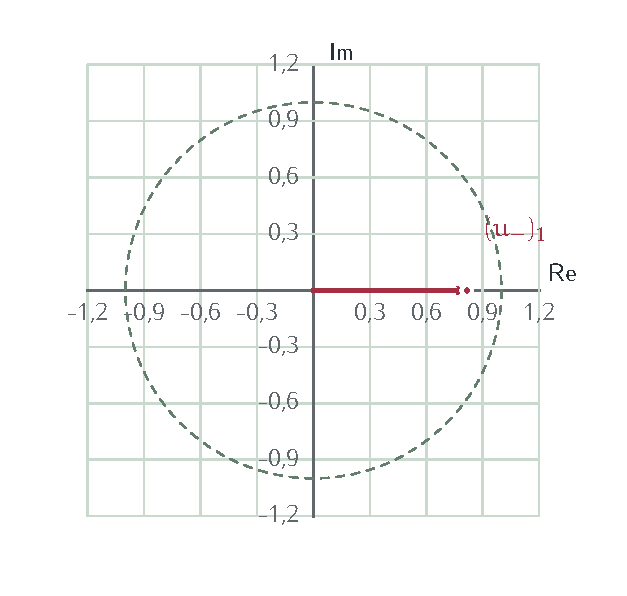
\includegraphics[width=\linewidth,height=63mm,keepaspectratio]{figure/f7c99497c94e24eb5.pdf}\par{\sffamily\footnotesize \((u_{-})_{1}\)\par}\end{minipage}\FigureCaption{2.28 \(\cdot\) esempio 2 \(\cdot\) Autovettori della base di misura}\end{FigureBlock}
\begin{FigureBlock}\begin{minipage}[t]{.485\linewidth}\centering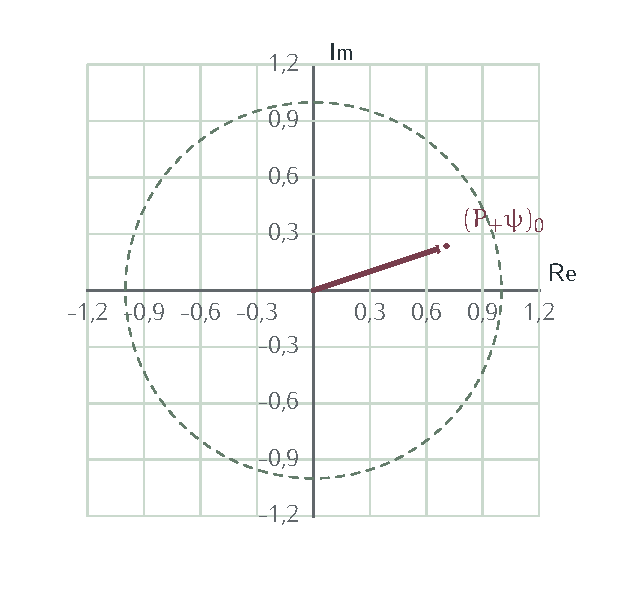
\includegraphics[width=\linewidth,height=63mm,keepaspectratio]{figure/f92adf633bde74ec8.pdf}\par{\sffamily\footnotesize \((P_{+}\psi )_{0}\)\par}\end{minipage}\hfill\begin{minipage}[t]{.485\linewidth}\centering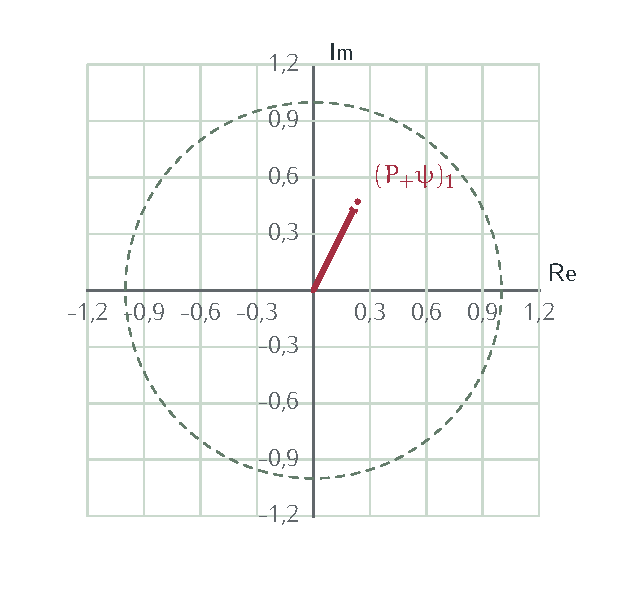
\includegraphics[width=\linewidth,height=63mm,keepaspectratio]{figure/fc47ed63d8b910776.pdf}\par{\sffamily\footnotesize \((P_{+}\psi )_{1}\)\par}\end{minipage}\FigureCaption{2.28 \(\cdot\) esempio 2 \(\cdot\) Proiezioni prima della rinormalizzazione}\end{FigureBlock}
\begin{FigureBlock}\begin{minipage}[t]{.485\linewidth}\centering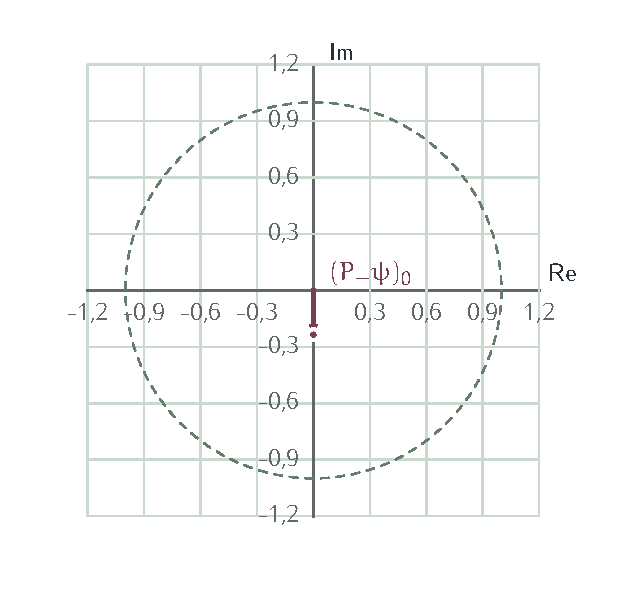
\includegraphics[width=\linewidth,height=63mm,keepaspectratio]{figure/f9a6c70f35f9d73c6.pdf}\par{\sffamily\footnotesize \((P_{-}\psi )_{0}\)\par}\end{minipage}\hfill\begin{minipage}[t]{.485\linewidth}\centering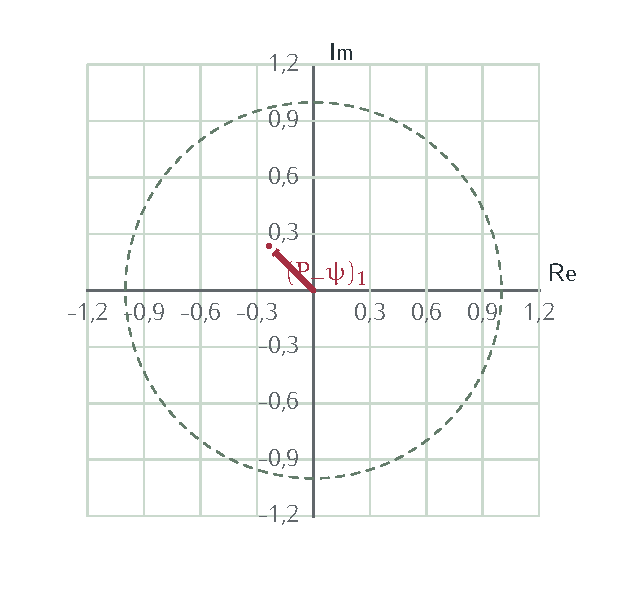
\includegraphics[width=\linewidth,height=63mm,keepaspectratio]{figure/f43c75775a48f08f7.pdf}\par{\sffamily\footnotesize \((P_{-}\psi )_{1}\)\par}\end{minipage}\FigureCaption{2.28 \(\cdot\) esempio 2 \(\cdot\) Proiezioni prima della rinormalizzazione}\end{FigureBlock}

\phantomsection\label{c2-esperimento-example-2-step-1}
\BookHeading{01 Controllare tutti i dati}

\MathBlock{0041003D005B005B0031002C003122120069005D002C005B0031002B0069002C0030005D005D}{A=\begin{pmatrix}1&1- i\\1+i&0\end{pmatrix}}
\MathBlock{00412020003D005B005B0031002C00280031002B00690029002A005D002C005B00280031221200690029002A002C0030005D005D003D0041}{A{}^{\dagger} =\begin{pmatrix}1&(1+i){}^{*}\\(1- i){}^{*}&0\end{pmatrix}=A}
\MathBlock{03C8003D00280031002C006900291D40002F221A0032003B0020201603C8201600B2003D00280031002B00310029002F0032003D0031}{\psi =(1,\allowbreak i)^{T}/\sqrt{2};\allowbreak \ \Vert \psi \Vert ^{2}=(1+1)/2=1}

La diagonale di \(A\) è reale e i termini fuori diagonale sono coniugati: \(A\) è un'osservabile hermitiana.\par


\phantomsection\label{c2-esperimento-example-2-step-2}
\BookHeading{02 Determinare gli autovalori}

\MathBlock{00640065007400280041221203BB00490029003D00280031221203BB00290028221203BB002922120028003122120069002900280031002B00690029}{\det (A- \lambda I)=(1- \lambda )(- \lambda )- (1- i)(1+i)}
\MathBlock{003D03BB00B2221203BB22120032003D002803BB221200320029002803BB002B00310029003D0030}{=\lambda ^{2}- \lambda - 2=(\lambda - 2)(\lambda +1)=0}
\MathBlock{03BB208A003D0032003B002003BB208B003D22120031}{\lambda _{+}=2;\allowbreak \ \lambda _{-}=- 1}

Il prodotto dei termini complessi vale \((1- i)(1+i)=2\).\par


\phantomsection\label{c2-esperimento-example-2-step-3}
\BookHeading{03 Risolvere il primo autovettore}

\MathBlock{03BB003D0032003A002022120078002B002800312212006900290079003D0030003B00200073006300650067006C00690061006D006F00200079003D0031002021D200200078003D003122120069}{\lambda =2:\ - x+(1- i)y=0;\allowbreak \ \text{scegliamo}\ y=1\ \Rightarrow \ x=1- i}
\MathBlock{00280031002B006900290028003122120069002922120032003D0030}{(1+i)(1- i)- 2=0}
\MathBlock{20160028003122120069002C00310029201600B2003D0032002B0031003D0033003B00200075208A003D0028003122120069002C003100291D40002F221A0033}{\Vert (1- i,\allowbreak 1)\Vert ^{2}=2+1=3;\allowbreak \ u_{+}=(1- i,\allowbreak 1)^{T}/\sqrt{3}}

Il candidato soddisfa entrambe le equazioni; dividere per \(\sqrt{3}\) lo normalizza.\par


\phantomsection\label{c2-esperimento-example-2-step-4}
\BookHeading{04 Risolvere il secondo autovettore}

\MathBlock{03BB003D22120031003A002000320078002B002800312212006900290079003D0030003B00200073006300650067006C00690061006D006F00200079003D0032002021D200200078003D22120031002B0069}{\lambda =- 1:\ 2x+(1- i)y=0;\allowbreak \ \text{scegliamo}\ y=2\ \Rightarrow \ x=- 1+i}
\MathBlock{00280031002B00690029002822120031002B00690029002B0032003D0030}{(1+i)(- 1+i)+2=0}
\MathBlock{2016002822120031002B0069002C00320029201600B2003D0032002B0034003D0036003B00200075208B003D002822120031002B0069002C003200291D40002F221A0036}{\Vert (- 1+i,\allowbreak 2)\Vert ^{2}=2+4=6;\allowbreak \ u_{-}=(- 1+i,\allowbreak 2)^{T}/\sqrt{6}}

Gli autovalori distinti individuano due autospazi di dimensione uno.\par


\phantomsection\label{c2-esperimento-example-2-step-5}
\BookHeading{05 Verificare l'ortogonalità}

\MathBlock{27E80075208A007C0075208B27E9003D005B00280031002B00690029002822120031002B00690029002B0032005D002F221A00310038003D002822120032002B00320029002F221A00310038003D0030}{\langle u_{+}|u_{-}\rangle =[(1+i)(- 1+i)+2]/\sqrt{18}=(- 2+2)/\sqrt{18}=0}

I due vettori normalizzati costituiscono una base ortonormale di \(C^{2}\).\par


\phantomsection\label{c2-esperimento-example-2-step-6}
\BookHeading{06 Calcolare le ampiezze esatte}

\MathBlock{0061208A003D005B00280031002B0069002900B70031002B0069005D002F221A0036003D00280031002B003200690029002F221A0036}{a_{+}=[(1+i)\cdot 1+i]/\sqrt{6}=(1+2i)/\sqrt{6}}
\MathBlock{0061208B003D005B00282212003122120069002900B70031002B00320069005D002F221A00310032003D002822120031002B00690029002F221A00310032}{a_{-}=[(- 1- i)\cdot 1+2i]/\sqrt{12}=(- 1+i)/\sqrt{12}}

I bra degli autovettori coniugano la prima componente prima del prodotto.\par


\phantomsection\label{c2-esperimento-example-2-step-7}
\BookHeading{07 Calcolare e sommare i moduli quadri}

\MathBlock{0070208A003D0028003100B2002B003200B20029002F0036003D0035002F0036003B00200070208B003D0028002822120031002900B2002B003100B20029002F00310032003D0031002F0036}{p_{+}=(1^{2}+2^{2})/6=5/6;\allowbreak \ p_{-}=((- 1)^{2}+1^{2})/12=1/6}
\MathBlock{0070208A002B0070208B003D0031}{p_{+}+p_{-}=1}

Le due probabilità coprono tutti gli esiti della misura.\par


\phantomsection\label{c2-esperimento-example-2-step-8}
\BookHeading{08 Proiettare nel ramo +}

\MathBlock{0050002B03C8003D0075002B0061002B224800280030002C00370030003700310020002B00200030002C00320033003500370069003B00200030002C00320033003500370020002B00200030002C0034003700310034006900291D40}{P+\psi =u+a+\approx (0{,}7071\ +\ 0{,}2357i;\allowbreak \ 0{,}2357\ +\ 0{,}4714i)^{T}}
\MathBlock{03C8002B003D0050002B03C8002F221A0070002B224800280030002C00370037003400360020002B00200030002C00320035003800320069003B00200030002C00320035003800320020002B00200030002C0035003100360034006900291D40}{\psi +=P+\psi /\sqrt{p}+\approx (0{,}7746\ +\ 0{,}2582i;\allowbreak \ 0{,}2582\ +\ 0{,}5164i)^{T}}

Il ramo è possibile perché il suo peso è positivo. Lo stato condizionato ha norma uno e appartiene al relativo autospazio.\par


\phantomsection\label{c2-esperimento-example-2-step-9}
\BookHeading{09 Proiettare nel ramo \(- \)}

\MathBlock{0050221203C8003D007522120061221222480028002D0030002C00320033003500370069003B0020002D0030002C00320033003500370020002B00200030002C0032003300350037006900291D40}{P- \psi =u- a- \approx (-0{,}2357i;\allowbreak \ -0{,}2357\ +\ 0{,}2357i)^{T}}
\MathBlock{03C82212003D0050221203C8002F221A0070221222480028002D0030002C00350037003700340069003B0020002D0030002C00350037003700340020002B00200030002C0035003700370034006900291D40}{\psi - =P- \psi /\sqrt{p}- \approx (-0{,}5774i;\allowbreak \ -0{,}5774\ +\ 0{,}5774i)^{T}}

Il ramo è possibile perché il suo peso è positivo. Lo stato condizionato ha norma uno e appartiene al relativo autospazio.\par


\phantomsection\label{c2-esperimento-example-2-step-10}
\BookHeading{10 Calcolare i momenti dallo spettro}

\MathBlock{27E8004127E9003D003200B70035002F003622120031002F0036003D0033002F0032}{\langle A\rangle =2\cdot 5/6- 1/6=3/2}
\MathBlock{27E8004100B227E9003D003400B70035002F0036002B0031002F0036003D0037002F0032}{\langle A^{2}\rangle =4\cdot 5/6+1/6=7/2}
\MathBlock{005600610072002800410029003D0037002F0032221200280033002F0032002900B2003D0035002F0034}{\operatorname{Var}(A)=7/2- (3/2)^{2}=5/4}

Si pesano prima gli esiti, poi i loro quadrati; la varianza sottrae il quadrato della media.\par


\phantomsection\label{c2-esperimento-example-2-step-11}
\BookHeading{11 Verifica \(A\psi \), riga 1}

\MathBlock{00280031002900B700280030002C003700300037003100290020002B0020002800310020221200200069002900B700280030002C00370030003700310069002922480031002C00340031003400320020002B00200030002C00370030003700310069}{(1)\cdot (0{,}7071)\ +\ (1\ - \ i)\cdot (0{,}7071i)\approx 1{,}4142\ +\ 0{,}7071i}

Ogni riga usa direttamente la preparazione normalizzata.\par


\phantomsection\label{c2-esperimento-example-2-step-12}
\BookHeading{12 Verifica \(A\psi \), riga 2}

\MathBlock{002800310020002B00200069002900B700280030002C003700300037003100290020002B002000280030002900B700280030002C00370030003700310069002922480030002C00370030003700310020002B00200030002C00370030003700310069}{(1\ +\ i)\cdot (0{,}7071)\ +\ (0)\cdot (0{,}7071i)\approx 0{,}7071\ +\ 0{,}7071i}

Ogni riga usa direttamente la preparazione normalizzata.\par


\phantomsection\label{c2-esperimento-example-2-step-13}
\BookHeading{13 Verifica \(A^{2}\psi \), riga 1}

\MathBlock{00280031002900B700280031002C00340031003400320020002B00200030002C0037003000370031006900290020002B0020002800310020221200200069002900B700280030002C00370030003700310020002B00200030002C00370030003700310069002922480032002C00380032003800340020002B00200030002C00370030003700310069}{(1)\cdot (1{,}4142\ +\ 0{,}7071i)\ +\ (1\ - \ i)\cdot (0{,}7071\ +\ 0{,}7071i)\approx 2{,}8284\ +\ 0{,}7071i}

La seconda applicazione usa l'uscita \(A\psi \) appena ottenuta.\par


\phantomsection\label{c2-esperimento-example-2-step-14}
\BookHeading{14 Verifica \(A^{2}\psi \), riga 2}

\MathBlock{002800310020002B00200069002900B700280031002C00340031003400320020002B00200030002C0037003000370031006900290020002B002000280030002900B700280030002C00370030003700310020002B00200030002C00370030003700310069002922480030002C00370030003700310020002B00200032002C00310032003100330069}{(1\ +\ i)\cdot (1{,}4142\ +\ 0{,}7071i)\ +\ (0)\cdot (0{,}7071\ +\ 0{,}7071i)\approx 0{,}7071\ +\ 2{,}1213i}

La seconda applicazione usa l'uscita \(A\psi \) appena ottenuta.\par


\phantomsection\label{c2-esperimento-example-2-step-15}
\BookHeading{15 Confrontare i momenti matriciali}

\MathBlock{27E803C8007C004103C827E9003D00280030002C0037003000370031002900B700280031002C00340031003400320020002B00200030002C0037003000370031006900290020002B00200028002D0030002C00370030003700310069002900B700280030002C00370030003700310020002B00200030002C00370030003700310069002922480031002C0035}{\langle \psi |A\psi \rangle =(0{,}7071)\cdot (1{,}4142\ +\ 0{,}7071i)\ +\ (-0{,}7071i)\cdot (0{,}7071\ +\ 0{,}7071i)\approx 1{,}5}
\MathBlock{27E803C8007C004100B203C827E9003D00280030002C0037003000370031002900B700280032002C00380032003800340020002B00200030002C0037003000370031006900290020002B00200028002D0030002C00370030003700310069002900B700280030002C00370030003700310020002B00200032002C00310032003100330069002922480033002C0035}{\langle \psi |A^{2}\psi \rangle =(0{,}7071)\cdot (2{,}8284\ +\ 0{,}7071i)\ +\ (-0{,}7071i)\cdot (0{,}7071\ +\ 2{,}1213i)\approx 3{,}5}
\MathBlock{00560061007200280041002922480031002C00320035}{\operatorname{Var}(A)\approx 1{,}25}

I prodotti matriciali confermano le frazioni ricavate indipendentemente dallo spettro.\par


\BookHeading{Interpretazione}

\(A\) conserva autovalori e autovettori del primo caso. Cambiare \(\psi \) modifica i pesi in (5/6,1/6), la media in 3/2 e la varianza in 5/4.\par


\Needspace{7\baselineskip}
\BookHeading{Il passaggio successivo}
Il calcolo completo ha collegato stato, autospazi e risultati. Per estenderlo a due sistemi occorre costruire lo spazio congiunto mediante il prodotto tensoriale.\par


% Authoritative exercise source. Preserve all derivations and diagrams.

\ExerciseStart{G2.13}{Svolgere integralmente una misura di un'osservabile}{Collegamento}

\BookHeading{Problema, dati e obiettivo}

Misurare \(A=\begin{pmatrix}1&1\\1&-1\end{pmatrix}\) nello stato \(\ket0\). Calcolare esiti, probabilità, stati condizionati, media e varianza. Confrontare poi le sequenze A seguita da Z e Z seguita da A, conservando l’informazione sull’ordine.

\ExTheory{\ExRef{c2-osservabili}{2.26}; \ExRef{c2-incompatibilita}{2.27}; \ExRef{c2-esperimento}{2.28}}{Una misura proiettiva di A dà un autovalore \(a_j\) con probabilità \(p_j=\|P_j\psi\|^2\). Se \(p_j>0\), lo stato condizionato è \(P_j\psi/\sqrt{p_j}\). Per una sequenza si applica la seconda regola di Born allo stato del ramo della prima misura.}

\ExPrediction{Le autodirezioni di A sono inclinate rispetto a quelle di Z. La prima misura di A dovrebbe quindi rendere possibile un successivo esito Z negativo, anche se la preparazione iniziale è \(\ket0\).}

\ExFigure{\begin{tikzpicture}[>=Stealth,exlabel]
\draw[exaxis] (-0.732683,0)--(1.55,0) node[right] {$x_1$};\draw[exaxis] (0,-0.35)--(0,1.47388) node[above] {$x_2$};\draw[->,Accent,line width=1.1pt] (0,0)--(0.92388,0.382683) node[anchor=south west] {$ u_+ $};\draw[->,Secondary,line width=1.1pt] (0,0)--(-0.382683,0.92388) node[anchor=south west] {$ u_- $};\draw[->,Ink,line width=1.1pt] (0,0)--(1,0) node[anchor=south west] {$ \ket0 $};
\end{tikzpicture}}{Piano reale delle ampiezze. L’angolo di \(u_+\) con \(\ket0\) è \(\pi/8\); il corrispondente angolo di Bloch è \(\pi/4\).}


\begin{ExTasks}

\item Calcolare gli autovalori e due autovettori ortonormali.

\item Proiettare \(\ket0\) e razionalizzare le probabilità.

\item Ricavare gli stati condizionati.

\item Calcolare media e varianza.

\item Costruire le quattro probabilità congiunte per A poi Z.

\item Ripetere per Z poi A e confrontare le marginali di Z.

\end{ExTasks}

\ExSolution

\ExStep{Risolvere lo spettro}

\ExEq{\det(A-\lambda I)&=(1-\lambda)(-1-\lambda)-1=\lambda^2-2.}
Gli autovalori sono \(\pm\sqrt2\). Posto \(t=\sqrt2-1\) e \(n=\sqrt{1+t^2}\), si scelgono \(u_+=(1,t)^T/n\) e \(u_-=(-t,1)^T/n\).

\ExStep{Verificare le autodirezioni}

Poiché \(t^2=3-2\sqrt2\), \(n^2=4-2\sqrt2\). Si ha
\ExEq{A\colv{1\\t}&=\colv{1+t\\1-t}=\sqrt2\colv{1\\t},\\A\colv{-t\\1}&=\colv{1-t\\-t-1}=-\sqrt2\colv{-t\\1}.}
Inoltre \(u_+^Tu_-=(-t+t)/n^2=0\) e le norme sono uno.

\ExStep{Calcolare le probabilità}

\ExEq{c_+&=\langle u_+|0\rangle=1/n,\quad c_-=-t/n,\\p_+&=\frac1{4-2\sqrt2}=\frac{4+2\sqrt2}{16-8}=\frac{2+\sqrt2}{4},\\p_-&=1-p_+=\frac{2-\sqrt2}{4}.}
La somma vale uno; entrambi gli esiti sono possibili.

\ExStep{Normalizzare i rami}

Per l’esito positivo, \(P_+\ket0=c_+u_+=u_+/n\); dividendo per \(\sqrt{p_+}=1/n\) si ottiene \(u_+\). Per l’esito negativo, \(P_-\ket0=-tu_-/n\), e \(\sqrt{p_-}=t/n\), poiché \(t>0\). Il risultato è \(-u_-\), equivalente fisicamente a \(u_-\) per la fase globale.

\ExStep{Calcolare i momenti}

\ExEq{\langle A\rangle&=\sqrt2(p_+-p_-)=\sqrt2\frac{2\sqrt2}{4}=1,\\\langle A^2\rangle&=2p_++2p_-=2,\\(\Delta A)^2&=2-1^2=1.}
Direttamente \(A^2=\begin{pmatrix}2&0\\0&2\end{pmatrix}\), in accordo con il secondo momento.

\ExStep{Eseguire A prima di Z}

Il ramo positivo ha probabilità di Z=+1 uguale a \(|(u_+)_0|^2=p_+\); il ramo negativo ha probabilità \(p_-\). Le quattro probabilità sono
\ExEq{P(A+,Z+)&=p_+^2=(3+2\sqrt2)/8,\\P(A+,Z-)&=p_+p_-=1/8,\\P(A-,Z+)&=p_-^2=(3-2\sqrt2)/8,\\P(A-,Z-)&=p_-p_+=1/8.}
Ne segue \(P(Z+)=6/8=3/4\) e \(P(Z-)=2/8=1/4\).

\ExStep{Eseguire Z prima di A}

La preparazione \(\ket0\) dà Z=+1 con probabilità uno e resta invariata. Quindi \(P(Z+,A+)=p_+\), \(P(Z+,A-)=p_-\), mentre i due eventi con Z negativo sono impossibili. La marginale di Z è ora \((1,0)\).

\ExStep{Collegare il risultato agli operatori}

\ExEq{AZ&=\begin{pmatrix}1&-1\\1&1\end{pmatrix},\quad ZA=\begin{pmatrix}1&1\\-1&1\end{pmatrix},\\{}[A,Z]&=\begin{pmatrix}0&-2\\2&0\end{pmatrix}\ne0.}
La prima misura modifica la preparazione disponibile alla seconda. Il confronto riguarda sequenze sullo stesso sistema, su molte copie della preparazione iniziale.

\par\noindent\begin{minipage}{\linewidth}
\ExFigure{\begin{tikzpicture}[>=Stealth,exlabel]
\draw[exaxis] (-.6,0)--(2.2,0) node[right] {esito};\draw[exaxis] (-.6,0)--(-.6,3.6) node[above] {$p$};\node[left] at (-.6,3) {$ 1 $};\draw[Ink!15,dashed] (-.6,3)--(1.7000000000000002,3);\filldraw[fill=Accent!25,draw=Accent] (0.0,0) rectangle (0.65,2.25);\node[below] at (0.325,0) {$ Z+  $};\node[above] at (0.325,2.25) {$ 0.75 $};\filldraw[fill=Accent!25,draw=Accent] (1.1,0) rectangle (1.75,0.75);\node[below] at (1.425,0) {$ Z- $};\node[above] at (1.425,0.75) {$ 0.25 $};
\end{tikzpicture}}{Marginale della seconda misura nella sequenza A poi Z.}


\ExInterpret{Gli autovalori sono i numeri restituiti dallo strumento; gli autovettori descrivono gli stati condizionati. Le probabilità congiunte mantengono esplicita la dipendenza dall’ordine delle misure.}

\ExLab{Nelle sezioni 2.26–2.28 confrontare spettro, proiezioni e sequenze di misura. Ricostruire ciascuna riga della tabella con il prodotto «probabilità del primo ramo per probabilità condizionata del secondo», usando l’esercizio come caso esatto di controllo.}


\end{minipage}

\Needspace{.43\textheight}
\section{Costruire le quattro ampiezze}
\phantomsection\label{c2-tensore}

{\sffamily\small\color{Ink!70} Riferimento alle slide: p. 167.\par}

{\sffamily\small\color{Ink!70} Laboratorio locale: \nolinkurl{index.html#capitolo-2/tensore}\par}

\BookHeading{Definizioni e costruzione}
Per descrivere due sistemi associamo a ogni coppia di etichette il prodotto delle componenti locali. Fissiamo l'ordine prima di calcolare.\par

Se il primo sistema ha due alternative e il secondo ne ha due, il sistema congiunto ha quattro etichette di base. La prima etichetta si riferisce sempre al primo sistema. Fissiamo l'ordine 00,01,10,11 prima di scrivere vettori e matrici.\par

Per una preparazione prodotto ogni ampiezza congiunta è il prodotto delle due ampiezze locali. Le norme si moltiplicano, così che due stati normalizzati producano uno stato congiunto normalizzato. Uno stato generale può richiedere quattro coefficienti che non ammettono questa fattorizzazione.\par


\MathBlock{002800612080002C0061208100291D402297002800622080002C0062208100291D40003D00280061208000622080002C0061208000622081002C0061208100622080002C006120810062208100291D40002E}{(a_{0},\allowbreak a_{1})^{T}\otimes (b_{0},\allowbreak b_{1})^{T}=(a_{0}b_{0},\allowbreak a_{0}b_{1},\allowbreak a_{1}b_{0},\allowbreak a_{1}b_{1})^{T}.}

\BookHeading{Come leggere le figure}
Base composta 00,01,10,11; quattro piani di ampiezza.\par


\Needspace{.36\textheight}\phantomsection\label{c2-tensore-example-1}
{\sffamily\small\color{Accent} ESEMPIO SVOLTO 1\par}
\BookHeading{Prodotto di due stati reali}
Dati \(a=(1{,}1)^{T}/\sqrt{2}\), \(b=(2{,}1)^{T}/\sqrt{5}\); ordine 00,01,10,11.\par


\BookHeading{Geometria e configurazione dell'esempio}
\begin{FigureBlock}\begin{minipage}[t]{.485\linewidth}\centering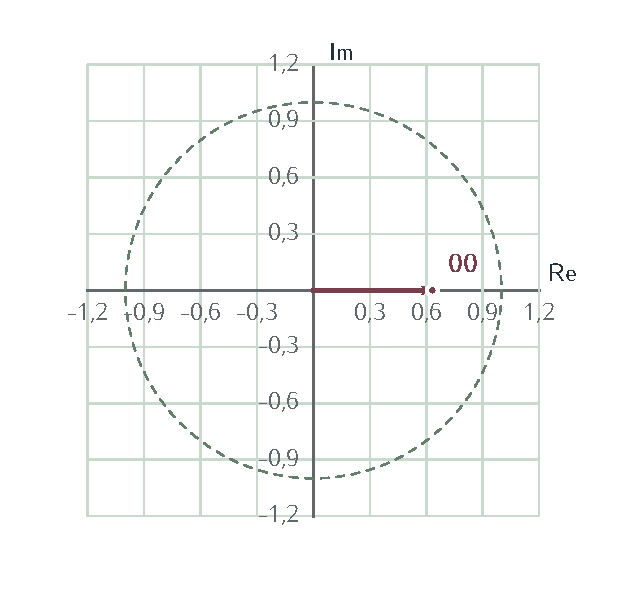
\includegraphics[width=\linewidth,height=63mm,keepaspectratio]{figure/f6cf9d979c8e24be2.pdf}\par{\sffamily\footnotesize 00\par}\end{minipage}\hfill\begin{minipage}[t]{.485\linewidth}\centering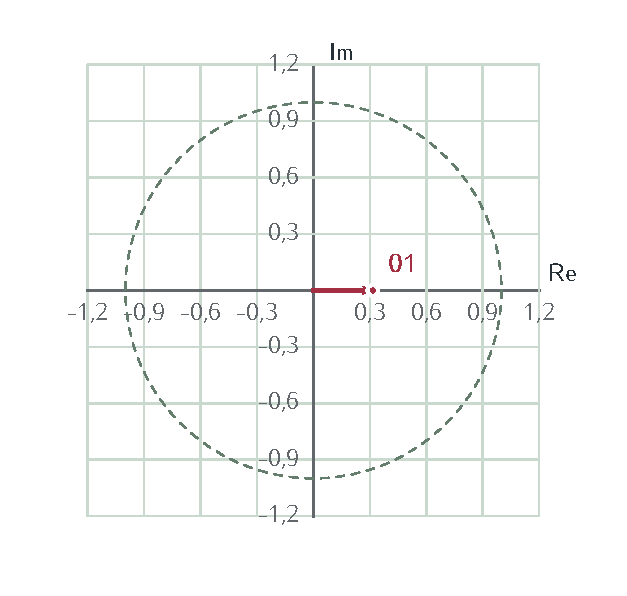
\includegraphics[width=\linewidth,height=63mm,keepaspectratio]{figure/f4f15c48e5a13ddd2.pdf}\par{\sffamily\footnotesize 01\par}\end{minipage}\FigureCaption{2.29 \(\cdot\) esempio 1 \(\cdot\) Quattro ampiezze costruite per prodotto}\end{FigureBlock}
\begin{FigureBlock}\begin{minipage}[t]{.485\linewidth}\centering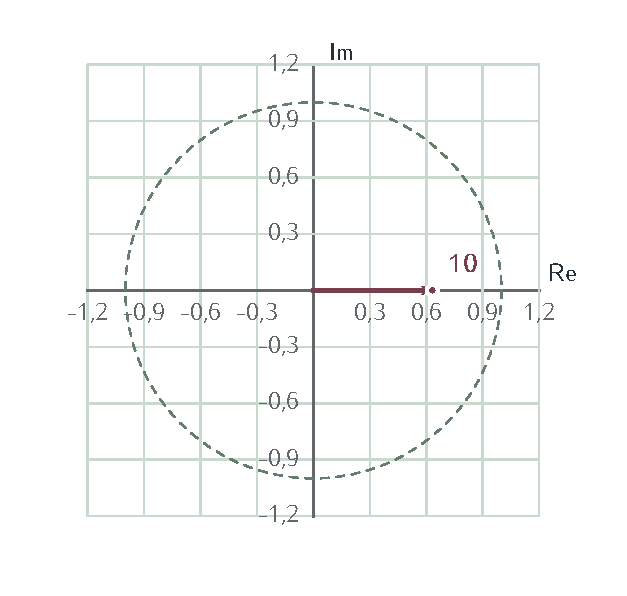
\includegraphics[width=\linewidth,height=63mm,keepaspectratio]{figure/f7afc9fad98e5ec05.pdf}\par{\sffamily\footnotesize 10\par}\end{minipage}\hfill\begin{minipage}[t]{.485\linewidth}\centering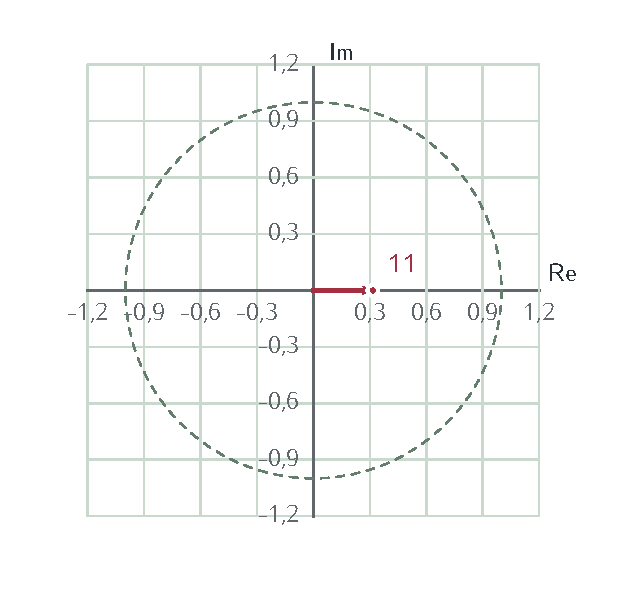
\includegraphics[width=\linewidth,height=63mm,keepaspectratio]{figure/fca71920ef7be7f36.pdf}\par{\sffamily\footnotesize 11\par}\end{minipage}\FigureCaption{2.29 \(\cdot\) esempio 1 \(\cdot\) Quattro ampiezze costruite per prodotto}\end{FigureBlock}
\begin{FigureBlock}\centering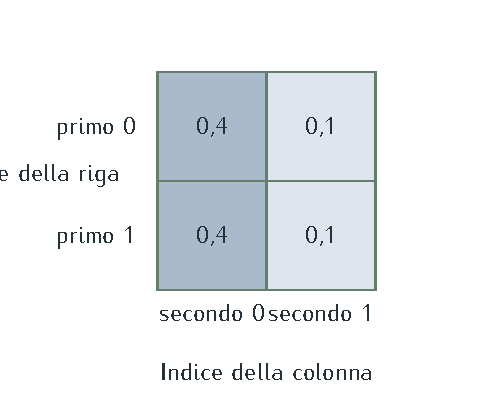
\includegraphics[width=\linewidth,height=94mm,keepaspectratio]{figure/f4a6545baf961a855.pdf}\FigureCaption{2.29 \(\cdot\) esempio 1 \(\cdot\) Probabilità del prodotto nella base \(Z\)}\end{FigureBlock}

\phantomsection\label{c2-tensore-example-1-step-1}
\BookHeading{01 Moltiplicare tutte le coppie di componenti}

\MathBlock{006300300030003D0061003000620030003D00280030002C0037003000370031002900280030002C0038003900340034002922480030002C0036003300320035}{c_{00}=a_{0}b_{0}=(0{,}7071)(0{,}8944)\approx 0{,}6325}
\MathBlock{006300300031003D0061003000620031003D00280030002C0037003000370031002900280030002C0034003400370032002922480030002C0033003100360032}{c_{01}=a_{0}b_{1}=(0{,}7071)(0{,}4472)\approx 0{,}3162}
\MathBlock{006300310030003D0061003100620030003D00280030002C0037003000370031002900280030002C0038003900340034002922480030002C0036003300320035}{c_{10}=a_{1}b_{0}=(0{,}7071)(0{,}8944)\approx 0{,}6325}
\MathBlock{006300310031003D0061003100620031003D00280030002C0037003000370031002900280030002C0034003400370032002922480030002C0033003100360032}{c_{11}=a_{1}b_{1}=(0{,}7071)(0{,}4472)\approx 0{,}3162}

Il primo indice percorre le righe; per ciascun suo valore il secondo indice percorre 0 e 1.\par


\phantomsection\label{c2-tensore-example-1-step-2}
\BookHeading{02 Verificare la norma prodotto}

\MathBlock{03A31D622C7C007C00611D6200622C7C007C00B2003D002803A31D62007C00611D62007C00B20029002803A32C7C007C00622C7C007C00B20029003D003100B70031003D0031}{\sum _{ij}|a_{i}b_{j}|^{2}=(\sum _{i}|a_{i}|^{2})(\sum _{j}|b_{j}|^{2})=1\cdot 1=1}
\MathBlock{03C8003D006122970062224800280030002C0036003300320035003B00200030002C0033003100360032003B00200030002C0036003300320035003B00200030002C003300310036003200291D40}{\psi =a\otimes b\approx (0{,}6325;\allowbreak \ 0{,}3162;\allowbreak \ 0{,}6325;\allowbreak \ 0{,}3162)^{T}}

La somma sui quattro coefficienti si fattorizza in due somme locali.\par


\phantomsection\label{c2-tensore-example-1-step-3}
\BookHeading{03 Scrivere l'espansione esatta nella base composta}

\MathBlock{03C8003D00280032007C0030003027E9002B007C0030003127E9002B0032007C0031003027E9002B007C0031003127E90029002F221A00310030}{\psi =(2|00\rangle +|01\rangle +2|10\rangle +|11\rangle )/\sqrt{10}}

Il denominatore \(\sqrt{2}\cdot \sqrt{5}=\sqrt{10}\) è comune ai quattro prodotti. L'espansione associa ogni coefficiente alla propria coppia di etichette.\par


\phantomsection\label{c2-tensore-example-1-step-4}
\BookHeading{04 Ricavare i pesi congiunti}

\MathBlock{005000300030003D007C006300300030007C00B222480030002C0034}{P_{00}=|c_{00}|^{2}\approx 0{,}4}
\MathBlock{005000300031003D007C006300300031007C00B222480030002C0031}{P_{01}=|c_{01}|^{2}\approx 0{,}1}
\MathBlock{005000310030003D007C006300310030007C00B222480030002C0034}{P_{10}=|c_{10}|^{2}\approx 0{,}4}
\MathBlock{005000310031003D007C006300310031007C00B222480030002C0031}{P_{11}=|c_{11}|^{2}\approx 0{,}1}

Una fase locale può cambiare le ampiezze senza cambiare questi pesi nella base \(Z\).\par


\BookHeading{Interpretazione}

Le quattro componenti sono \((2{,}1{,}2{,}1)/\sqrt{10}\); ogni coefficiente conserva l'informazione sull'ordine dei due sistemi.\par


\Needspace{.36\textheight}\phantomsection\label{c2-tensore-example-2}
{\sffamily\small\color{Accent} ESEMPIO SVOLTO 2\par}
\BookHeading{Fase locale nelle ampiezze congiunte}
Dati \(a=(1,\allowbreak i)^{T}/\sqrt{2}\), \(b=(2{,}1)^{T}/\sqrt{5}\); ordine 00,01,10,11.\par


\BookHeading{Geometria e configurazione dell'esempio}
\begin{FigureBlock}\begin{minipage}[t]{.485\linewidth}\centering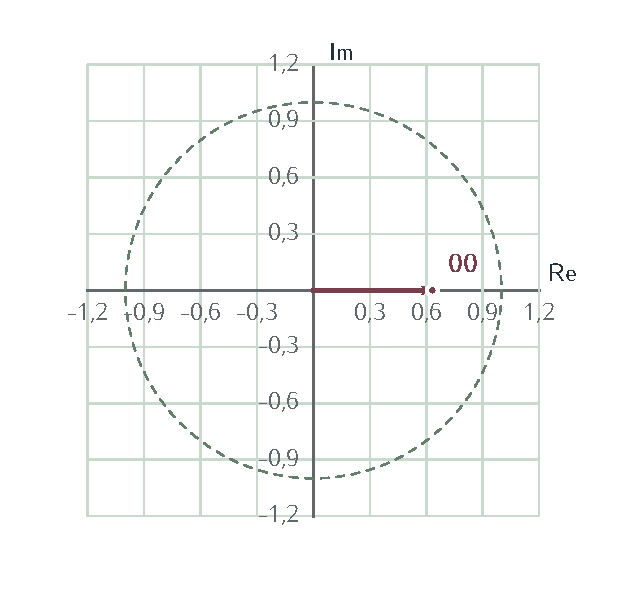
\includegraphics[width=\linewidth,height=63mm,keepaspectratio]{figure/f72c46f63503c9249.pdf}\par{\sffamily\footnotesize 00\par}\end{minipage}\hfill\begin{minipage}[t]{.485\linewidth}\centering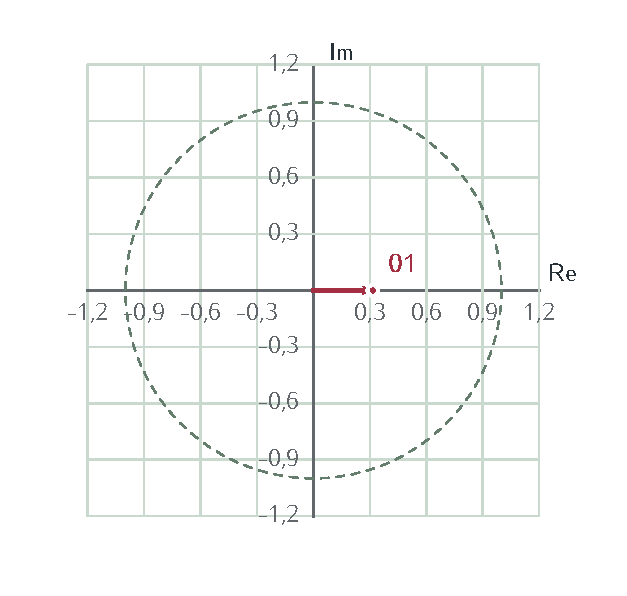
\includegraphics[width=\linewidth,height=63mm,keepaspectratio]{figure/ff55416265dc791f6.pdf}\par{\sffamily\footnotesize 01\par}\end{minipage}\FigureCaption{2.29 \(\cdot\) esempio 2 \(\cdot\) Quattro ampiezze costruite per prodotto}\end{FigureBlock}
\begin{FigureBlock}\begin{minipage}[t]{.485\linewidth}\centering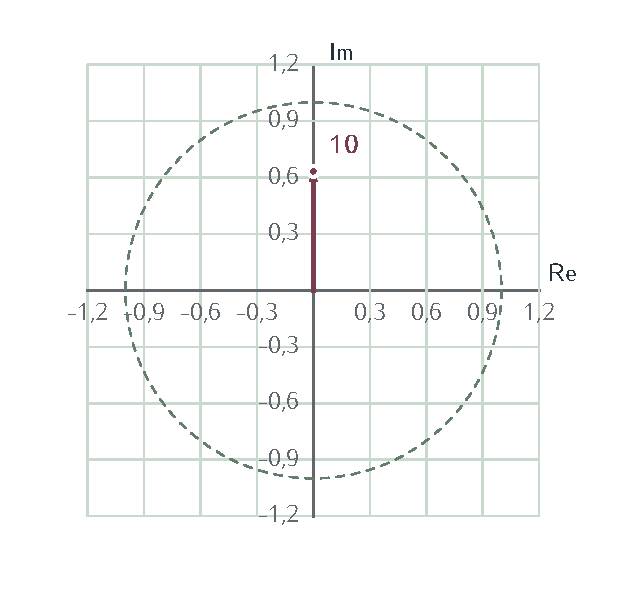
\includegraphics[width=\linewidth,height=63mm,keepaspectratio]{figure/f50117a498eda53b2.pdf}\par{\sffamily\footnotesize 10\par}\end{minipage}\hfill\begin{minipage}[t]{.485\linewidth}\centering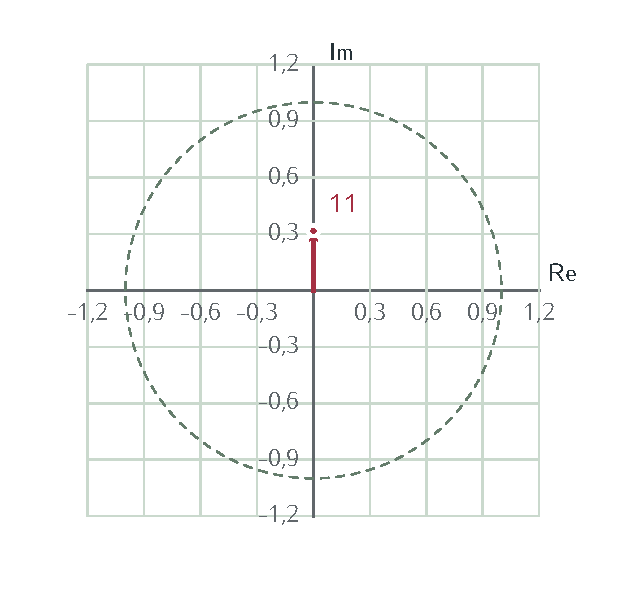
\includegraphics[width=\linewidth,height=63mm,keepaspectratio]{figure/f6c8ed70dc3f5d56b.pdf}\par{\sffamily\footnotesize 11\par}\end{minipage}\FigureCaption{2.29 \(\cdot\) esempio 2 \(\cdot\) Quattro ampiezze costruite per prodotto}\end{FigureBlock}
\begin{FigureBlock}\centering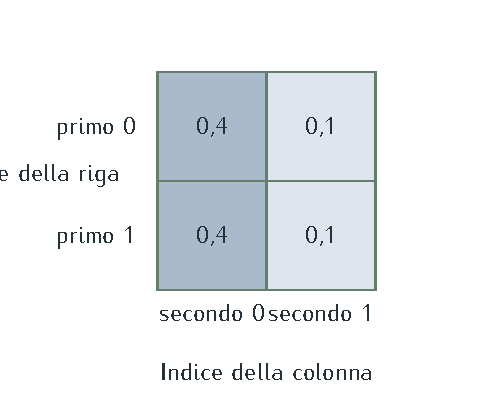
\includegraphics[width=\linewidth,height=94mm,keepaspectratio]{figure/f4a6545baf961a855.pdf}\FigureCaption{2.29 \(\cdot\) esempio 2 \(\cdot\) Probabilità del prodotto nella base \(Z\)}\end{FigureBlock}

\phantomsection\label{c2-tensore-example-2-step-1}
\BookHeading{01 Moltiplicare tutte le coppie di componenti}

\MathBlock{006300300030003D0061003000620030003D00280030002C0037003000370031002900280030002C0038003900340034002922480030002C0036003300320035}{c_{00}=a_{0}b_{0}=(0{,}7071)(0{,}8944)\approx 0{,}6325}
\MathBlock{006300300031003D0061003000620031003D00280030002C0037003000370031002900280030002C0034003400370032002922480030002C0033003100360032}{c_{01}=a_{0}b_{1}=(0{,}7071)(0{,}4472)\approx 0{,}3162}
\MathBlock{006300310030003D0061003100620030003D00280030002C00370030003700310069002900280030002C0038003900340034002922480030002C00360033003200350069}{c_{10}=a_{1}b_{0}=(0{,}7071i)(0{,}8944)\approx 0{,}6325i}
\MathBlock{006300310031003D0061003100620031003D00280030002C00370030003700310069002900280030002C0034003400370032002922480030002C00330031003600320069}{c_{11}=a_{1}b_{1}=(0{,}7071i)(0{,}4472)\approx 0{,}3162i}

Il primo indice percorre le righe; per ciascun suo valore il secondo indice percorre 0 e 1.\par


\phantomsection\label{c2-tensore-example-2-step-2}
\BookHeading{02 Verificare la norma prodotto}

\MathBlock{03A31D622C7C007C00611D6200622C7C007C00B2003D002803A31D62007C00611D62007C00B20029002803A32C7C007C00622C7C007C00B20029003D003100B70031003D0031}{\sum _{ij}|a_{i}b_{j}|^{2}=(\sum _{i}|a_{i}|^{2})(\sum _{j}|b_{j}|^{2})=1\cdot 1=1}
\MathBlock{03C8003D006122970062224800280030002C0036003300320035003B00200030002C0033003100360032003B00200030002C00360033003200350069003B00200030002C0033003100360032006900291D40}{\psi =a\otimes b\approx (0{,}6325;\allowbreak \ 0{,}3162;\allowbreak \ 0{,}6325i;\allowbreak \ 0{,}3162i)^{T}}

La somma sui quattro coefficienti si fattorizza in due somme locali.\par


\phantomsection\label{c2-tensore-example-2-step-3}
\BookHeading{03 Scrivere l'espansione esatta nella base composta}

\MathBlock{03C8003D00280032007C0030003027E9002B007C0030003127E9002B00320069007C0031003027E9002B0069007C0031003127E90029002F221A00310030}{\psi =(2|00\rangle +|01\rangle +2i|10\rangle +i|11\rangle )/\sqrt{10}}

Il denominatore \(\sqrt{2}\cdot \sqrt{5}=\sqrt{10}\) è comune ai quattro prodotti. L'espansione associa ogni coefficiente alla propria coppia di etichette.\par


\phantomsection\label{c2-tensore-example-2-step-4}
\BookHeading{04 Ricavare i pesi congiunti}

\MathBlock{005000300030003D007C006300300030007C00B222480030002C0034}{P_{00}=|c_{00}|^{2}\approx 0{,}4}
\MathBlock{005000300031003D007C006300300031007C00B222480030002C0031}{P_{01}=|c_{01}|^{2}\approx 0{,}1}
\MathBlock{005000310030003D007C006300310030007C00B222480030002C0034}{P_{10}=|c_{10}|^{2}\approx 0{,}4}
\MathBlock{005000310031003D007C006300310031007C00B222480030002C0031}{P_{11}=|c_{11}|^{2}\approx 0{,}1}

Una fase locale può cambiare le ampiezze senza cambiare questi pesi nella base \(Z\).\par


\BookHeading{Interpretazione}

La fase i del primo qubit compare nelle componenti 10 e 11. La distribuzione \(Z\) resta (2/5,1/10,2/5,1/10), come nel primo caso.\par


\Needspace{7\baselineskip}
\BookHeading{Il passaggio successivo}
Le quattro ampiezze conservano le due etichette locali. Le matrici \(X\otimes I\) e \(I\otimes X\) mostreranno come trasformare soltanto il sistema indicato.\par


\Needspace{.43\textheight}
\section{Agire su un solo sistema}
\phantomsection\label{c2-porte-locali}

{\sffamily\small\color{Ink!70} Riferimento alle slide: p. 167.\par}

{\sffamily\small\color{Ink!70} Laboratorio locale: \nolinkurl{index.html#capitolo-2/porte-locali}\par}

\BookHeading{Definizioni e costruzione}
Una porta locale modifica il qubit scelto e conserva l'etichetta dell'altro. La matrice prodotto tensoriale rende esplicita questa regola.\par

Una porta sul primo sistema agisce su tutte le ampiezze che condividono l'etichetta del secondo. Per ogni etichetta fissata del secondo qubit si applica la stessa matrice a due componenti. L'identità sul secondo fattore esprime precisamente questa conservazione.\par

Scrivere \(U\otimes I\) permette di verificare l'ordine dei fili e delle componenti. Una porta sul secondo sistema è invece \(I\otimes U\). Le due azioni possono essere confrontate su una preparazione prodotto e successivamente su uno stato entangled, mantenendo la descrizione congiunta.\par


\MathBlock{0028005522970049002900280061229700620029003D002800550061002922970062002E}{(U\otimes I)(a\otimes b)=(Ua)\otimes b.}

\BookHeading{Come leggere le figure}
Ampiezze congiunte in ordine 00,01,10,11.\par


\Needspace{.36\textheight}\phantomsection\label{c2-porte-locali-example-1}
{\sffamily\small\color{Accent} ESEMPIO SVOLTO 1\par}
\BookHeading{Due qubit, due scambi distinti}
Dati \(a=(1{,}2)^{T}/\sqrt{5}\), \(b=(2{,}1)^{T}/\sqrt{5}\); ordine 00,01,10,11.\par


\BookHeading{Geometria e configurazione dell'esempio}
\begin{FigureBlock}\begin{minipage}[t]{.485\linewidth}\centering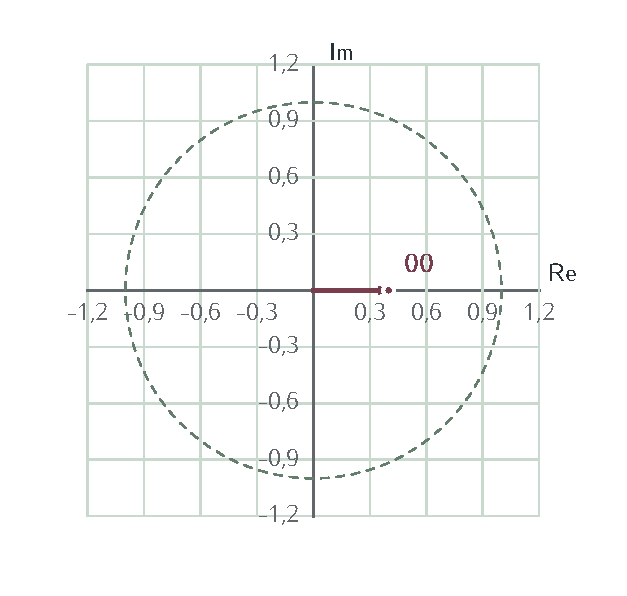
\includegraphics[width=\linewidth,height=63mm,keepaspectratio]{figure/f6cc709a4e7b926a3.pdf}\par{\sffamily\footnotesize 00\par}\end{minipage}\hfill\begin{minipage}[t]{.485\linewidth}\centering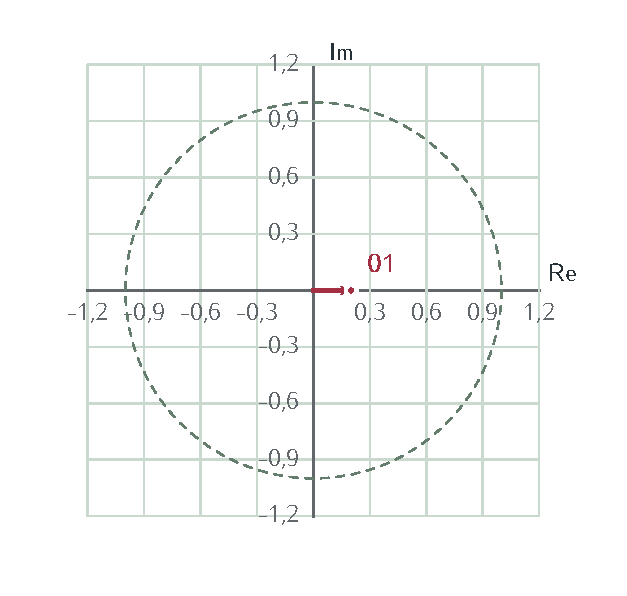
\includegraphics[width=\linewidth,height=63mm,keepaspectratio]{figure/f0adb80ea70c2207a.pdf}\par{\sffamily\footnotesize 01\par}\end{minipage}\FigureCaption{2.30 \(\cdot\) esempio 1 \(\cdot\) Prima delle porte locali}\end{FigureBlock}
\begin{FigureBlock}\begin{minipage}[t]{.485\linewidth}\centering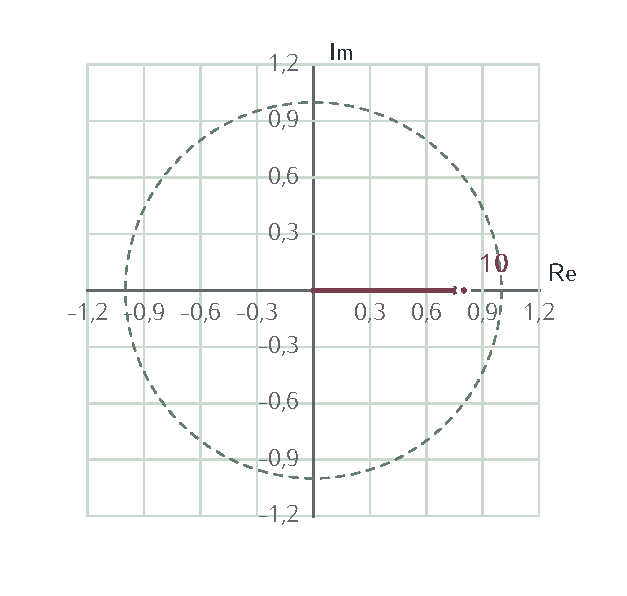
\includegraphics[width=\linewidth,height=63mm,keepaspectratio]{figure/f28ae4450ac20e804.pdf}\par{\sffamily\footnotesize 10\par}\end{minipage}\hfill\begin{minipage}[t]{.485\linewidth}\centering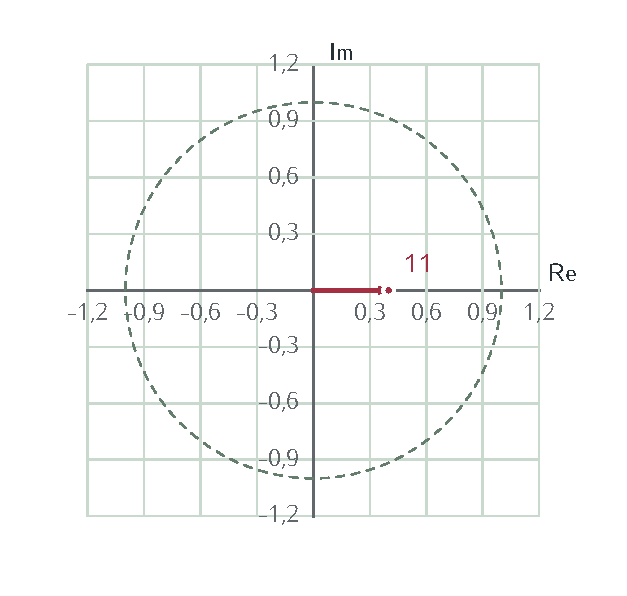
\includegraphics[width=\linewidth,height=63mm,keepaspectratio]{figure/ffaebd4df1e6fbb1f.pdf}\par{\sffamily\footnotesize 11\par}\end{minipage}\FigureCaption{2.30 \(\cdot\) esempio 1 \(\cdot\) Prima delle porte locali}\end{FigureBlock}
\begin{FigureBlock}\begin{minipage}[t]{.485\linewidth}\centering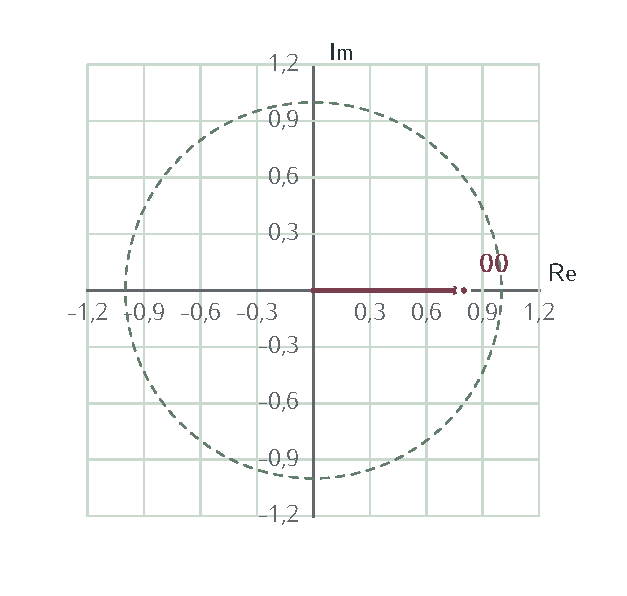
\includegraphics[width=\linewidth,height=63mm,keepaspectratio]{figure/ff8d98b4081295f6a.pdf}\par{\sffamily\footnotesize 00\par}\end{minipage}\hfill\begin{minipage}[t]{.485\linewidth}\centering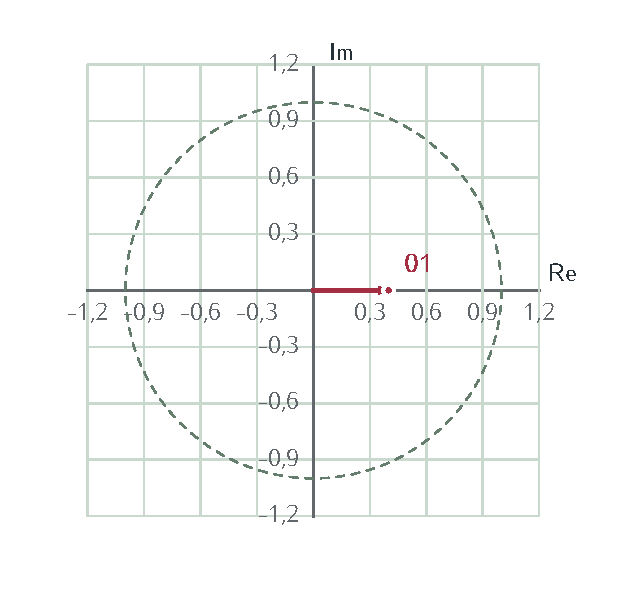
\includegraphics[width=\linewidth,height=63mm,keepaspectratio]{figure/f8daf65a1ec0886c8.pdf}\par{\sffamily\footnotesize 01\par}\end{minipage}\FigureCaption{2.30 \(\cdot\) esempio 1 \(\cdot\) Dopo \(X\) sul primo qubit}\end{FigureBlock}
\begin{FigureBlock}\begin{minipage}[t]{.485\linewidth}\centering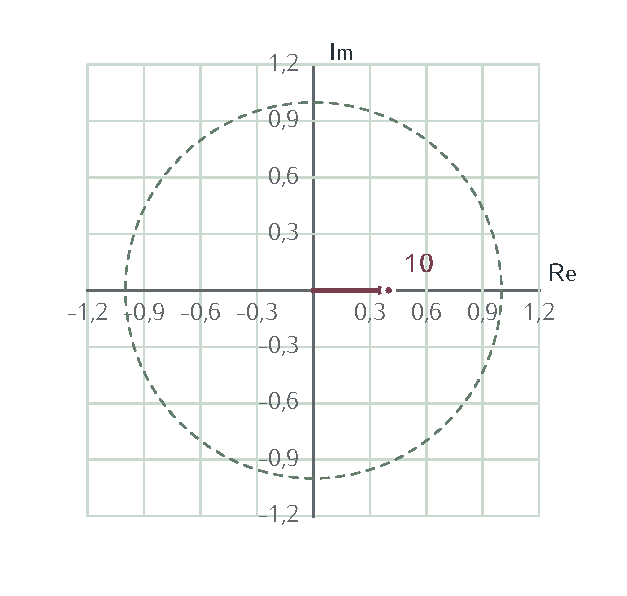
\includegraphics[width=\linewidth,height=63mm,keepaspectratio]{figure/fcdc80e4812b945d5.pdf}\par{\sffamily\footnotesize 10\par}\end{minipage}\hfill\begin{minipage}[t]{.485\linewidth}\centering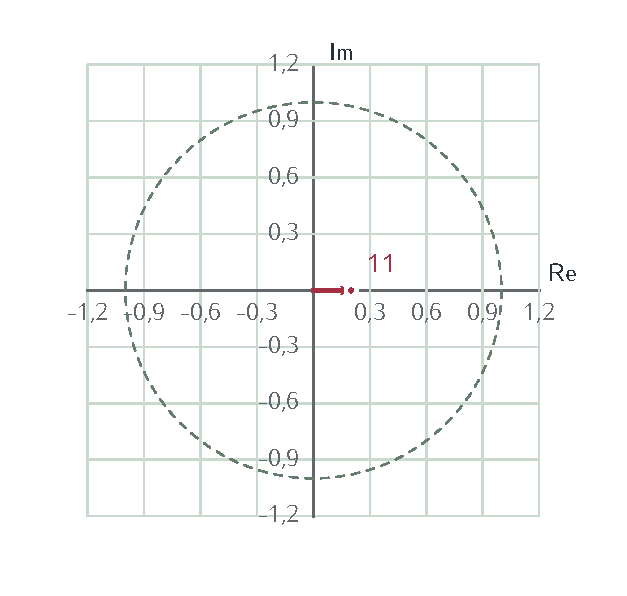
\includegraphics[width=\linewidth,height=63mm,keepaspectratio]{figure/fdc868b240b52f684.pdf}\par{\sffamily\footnotesize 11\par}\end{minipage}\FigureCaption{2.30 \(\cdot\) esempio 1 \(\cdot\) Dopo \(X\) sul primo qubit}\end{FigureBlock}
\begin{FigureBlock}\begin{minipage}[t]{.485\linewidth}\centering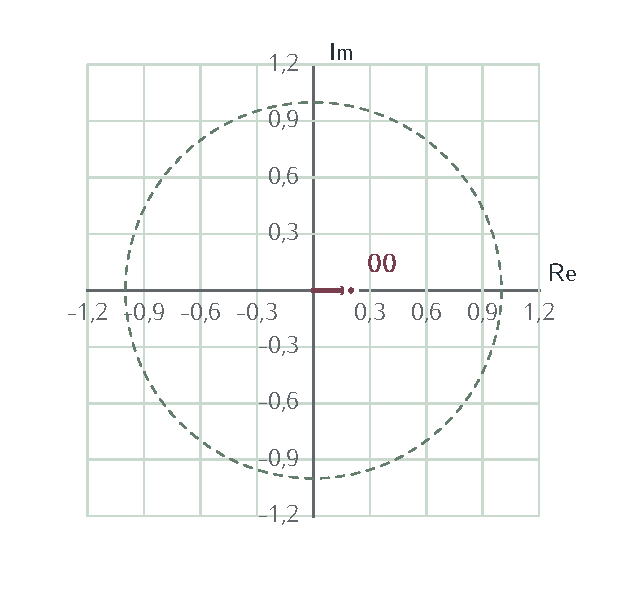
\includegraphics[width=\linewidth,height=63mm,keepaspectratio]{figure/fd2a3f4ca6533bd87.pdf}\par{\sffamily\footnotesize 00\par}\end{minipage}\hfill\begin{minipage}[t]{.485\linewidth}\centering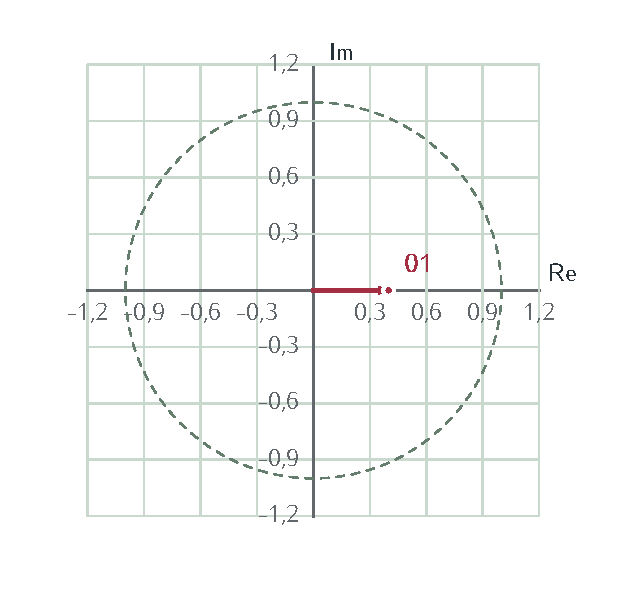
\includegraphics[width=\linewidth,height=63mm,keepaspectratio]{figure/f3ee260ce60c72059.pdf}\par{\sffamily\footnotesize 01\par}\end{minipage}\FigureCaption{2.30 \(\cdot\) esempio 1 \(\cdot\) Dopo \(X\) sul secondo qubit}\end{FigureBlock}
\begin{FigureBlock}\begin{minipage}[t]{.485\linewidth}\centering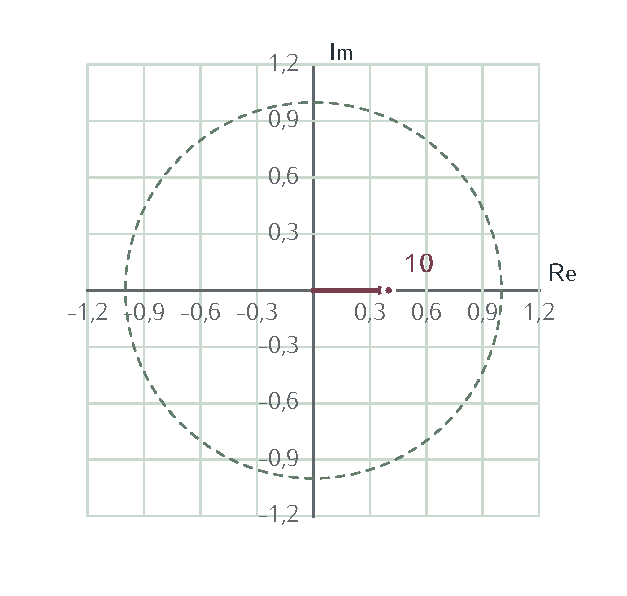
\includegraphics[width=\linewidth,height=63mm,keepaspectratio]{figure/fef15c542bc09703f.pdf}\par{\sffamily\footnotesize 10\par}\end{minipage}\hfill\begin{minipage}[t]{.485\linewidth}\centering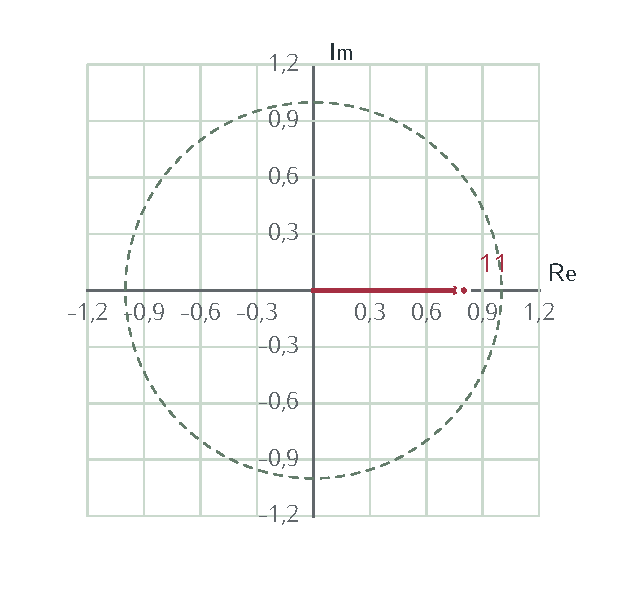
\includegraphics[width=\linewidth,height=63mm,keepaspectratio]{figure/f0c62099dd581fbd4.pdf}\par{\sffamily\footnotesize 11\par}\end{minipage}\FigureCaption{2.30 \(\cdot\) esempio 1 \(\cdot\) Dopo \(X\) sul secondo qubit}\end{FigureBlock}

\phantomsection\label{c2-porte-locali-example-1-step-1}
\BookHeading{01 Moltiplicare tutte le coppie di componenti}

\MathBlock{006300300030003D0061003000620030003D00280030002C0034003400370032002900280030002C0038003900340034002922480030002C0034}{c_{00}=a_{0}b_{0}=(0{,}4472)(0{,}8944)\approx 0{,}4}
\MathBlock{006300300031003D0061003000620031003D00280030002C0034003400370032002900280030002C0034003400370032002922480030002C0032}{c_{01}=a_{0}b_{1}=(0{,}4472)(0{,}4472)\approx 0{,}2}
\MathBlock{006300310030003D0061003100620030003D00280030002C0038003900340034002900280030002C0038003900340034002922480030002C0038}{c_{10}=a_{1}b_{0}=(0{,}8944)(0{,}8944)\approx 0{,}8}
\MathBlock{006300310031003D0061003100620031003D00280030002C0038003900340034002900280030002C0034003400370032002922480030002C0034}{c_{11}=a_{1}b_{1}=(0{,}8944)(0{,}4472)\approx 0{,}4}

Il primo indice percorre le righe; per ciascun suo valore il secondo indice percorre 0 e 1.\par


\phantomsection\label{c2-porte-locali-example-1-step-2}
\BookHeading{02 Verificare la norma prodotto}

\MathBlock{03A31D622C7C007C00611D6200622C7C007C00B2003D002803A31D62007C00611D62007C00B20029002803A32C7C007C00622C7C007C00B20029003D003100B70031003D0031}{\sum _{ij}|a_{i}b_{j}|^{2}=(\sum _{i}|a_{i}|^{2})(\sum _{j}|b_{j}|^{2})=1\cdot 1=1}
\MathBlock{03C8003D006122970062224800280030002C0034003B00200030002C0032003B00200030002C0038003B00200030002C003400291D40}{\psi =a\otimes b\approx (0{,}4;\allowbreak \ 0{,}2;\allowbreak \ 0{,}8;\allowbreak \ 0{,}4)^{T}}

La somma sui quattro coefficienti si fattorizza in due somme locali.\par


\phantomsection\label{c2-porte-locali-example-1-step-3}
\BookHeading{03 Scrivere le due azioni locali}

\MathBlock{0058003D005B005B0030002C0031005D002C005B0031002C0030005D005D}{X=\begin{pmatrix}0&1\\1&0\end{pmatrix}}
\MathBlock{005822970049003D005B005B0030002C0030002C0031002C0030005D002C005B0030002C0030002C0030002C0031005D002C005B0031002C0030002C0030002C0030005D002C005B0030002C0031002C0030002C0030005D005D}{X\otimes I=\begin{pmatrix}0&0&1&0\\0&0&0&1\\1&0&0&0\\0&1&0&0\end{pmatrix}}
\MathBlock{004922970058003D005B005B0030002C0031002C0030002C0030005D002C005B0031002C0030002C0030002C0030005D002C005B0030002C0030002C0030002C0031005D002C005B0030002C0030002C0031002C0030005D005D}{I\otimes X=\begin{pmatrix}0&1&0&0\\1&0&0&0\\0&0&0&1\\0&0&1&0\end{pmatrix}}

\(X\) sul primo qubit scambia \(00\leftrightarrow 10\) e \(01\leftrightarrow 11\); \(X\) sul secondo scambia \(00\leftrightarrow 01\) e \(10\leftrightarrow 11\).\par


\phantomsection\label{c2-porte-locali-example-1-step-4}
\BookHeading{04 Seguire tutti gli scambi}

\MathBlock{0028005822970049002903C8003A00200063203200300030003D00630031003022480030002C0038003B00200028004922970058002903C8003A00200064203200300030003D00630030003122480030002C0032}{(X\otimes I)\psi :\ c{}^{\prime} 00=c_{10}\approx 0{,}8;\allowbreak \ (I\otimes X)\psi :\ d{}^{\prime} 00=c_{01}\approx 0{,}2}
\MathBlock{0028005822970049002903C8003A00200063203200300031003D00630031003122480030002C0034003B00200028004922970058002903C8003A00200064203200300031003D00630030003022480030002C0034}{(X\otimes I)\psi :\ c{}^{\prime} 01=c_{11}\approx 0{,}4;\allowbreak \ (I\otimes X)\psi :\ d{}^{\prime} 01=c_{00}\approx 0{,}4}
\MathBlock{0028005822970049002903C8003A00200063203200310030003D00630030003022480030002C0034003B00200028004922970058002903C8003A00200064203200310030003D00630031003122480030002C0034}{(X\otimes I)\psi :\ c{}^{\prime} 10=c_{00}\approx 0{,}4;\allowbreak \ (I\otimes X)\psi :\ d{}^{\prime} 10=c_{11}\approx 0{,}4}
\MathBlock{0028005822970049002903C8003A00200063203200310031003D00630030003122480030002C0032003B00200028004922970058002903C8003A00200064203200310031003D00630031003022480030002C0038}{(X\otimes I)\psi :\ c{}^{\prime} 11=c_{01}\approx 0{,}2;\allowbreak \ (I\otimes X)\psi :\ d{}^{\prime} 11=c_{10}\approx 0{,}8}

La componente nuova viene copiata dalla componente con il bit scelto invertito.\par


\phantomsection\label{c2-porte-locali-example-1-step-5}
\BookHeading{05 Verificare attraverso i fattori}

\MathBlock{00580061003D00280030002C0038003900340034003B00200030002C003400340037003200291D40003B002000580062003D00280030002C0034003400370032003B00200030002C003800390034003400291D40}{Xa=(0{,}8944;\allowbreak \ 0{,}4472)^{T};\allowbreak \ Xb=(0{,}4472;\allowbreak \ 0{,}8944)^{T}}
\MathBlock{002800580061002922970062003D00280030002C0038003B00200030002C0034003B00200030002C0034003B00200030002C003200291D40}{(Xa)\otimes b=(0{,}8;\allowbreak \ 0{,}4;\allowbreak \ 0{,}4;\allowbreak \ 0{,}2)^{T}}
\MathBlock{006122970028005800620029003D00280030002C0032003B00200030002C0034003B00200030002C0034003B00200030002C003800291D40}{a\otimes (Xb)=(0{,}2;\allowbreak \ 0{,}4;\allowbreak \ 0{,}4;\allowbreak \ 0{,}8)^{T}}

Il calcolo a quattro componenti coincide con l'azione sulla sola preparazione locale interessata.\par


\phantomsection\label{c2-porte-locali-example-1-step-6}
\BookHeading{06 Controllare la norma e il caso invariante}

\MathBlock{20160028005822970049002903C8201600B2003D20160028004922970058002903C8201600B2003D0031}{\Vert (X\otimes I)\psi \Vert ^{2}=\Vert (I\otimes X)\psi \Vert ^{2}=1}
\MathBlock{0058007C002B27E9003D00280031002C003100291D40002F221A0032003D007C002B27E9}{X|+\rangle =(1{,}1)^{T}/\sqrt{2}=|+\rangle }

I dati scelti rendono visibili gli scambi; una preparazione \(|+\rangle \) sul qubit trasformato sarebbe invece invariante.\par


\BookHeading{Interpretazione}

I due operatori agiscono su coppie diverse di componenti. Il confronto dei prodotti verifica quale qubit sia stato trasformato.\par


\Needspace{.36\textheight}\phantomsection\label{c2-porte-locali-example-2}
{\sffamily\small\color{Accent} ESEMPIO SVOLTO 2\par}
\BookHeading{Scambio locale di ampiezze con fase}
Dati \(a=(1{,}2i)^{T}/\sqrt{5}\), \(b=(2{,}1)^{T}/\sqrt{5}\); ordine 00,01,10,11.\par


\BookHeading{Geometria e configurazione dell'esempio}
\begin{FigureBlock}\begin{minipage}[t]{.485\linewidth}\centering\includegraphics[width=\linewidth,height=63mm,keepaspectratio]{figure/fd764a70b7e7c1043.pdf}\par{\sffamily\footnotesize 00\par}\end{minipage}\hfill\begin{minipage}[t]{.485\linewidth}\centering\includegraphics[width=\linewidth,height=63mm,keepaspectratio]{figure/f45845de508f34dbc.pdf}\par{\sffamily\footnotesize 01\par}\end{minipage}\FigureCaption{2.30 \(\cdot\) esempio 2 \(\cdot\) Prima delle porte locali}\end{FigureBlock}
\begin{FigureBlock}\begin{minipage}[t]{.485\linewidth}\centering\includegraphics[width=\linewidth,height=63mm,keepaspectratio]{figure/f2df85bfc3dd0b5df.pdf}\par{\sffamily\footnotesize 10\par}\end{minipage}\hfill\begin{minipage}[t]{.485\linewidth}\centering\includegraphics[width=\linewidth,height=63mm,keepaspectratio]{figure/f25e704022f1b4f29.pdf}\par{\sffamily\footnotesize 11\par}\end{minipage}\FigureCaption{2.30 \(\cdot\) esempio 2 \(\cdot\) Prima delle porte locali}\end{FigureBlock}
\begin{FigureBlock}\begin{minipage}[t]{.485\linewidth}\centering\includegraphics[width=\linewidth,height=63mm,keepaspectratio]{figure/fe62fdeae923cc8e1.pdf}\par{\sffamily\footnotesize 00\par}\end{minipage}\hfill\begin{minipage}[t]{.485\linewidth}\centering\includegraphics[width=\linewidth,height=63mm,keepaspectratio]{figure/f581b23511ab3eea4.pdf}\par{\sffamily\footnotesize 01\par}\end{minipage}\FigureCaption{2.30 \(\cdot\) esempio 2 \(\cdot\) Dopo \(X\) sul primo qubit}\end{FigureBlock}
\begin{FigureBlock}\begin{minipage}[t]{.485\linewidth}\centering\includegraphics[width=\linewidth,height=63mm,keepaspectratio]{figure/ff9f5c77e92be4914.pdf}\par{\sffamily\footnotesize 10\par}\end{minipage}\hfill\begin{minipage}[t]{.485\linewidth}\centering\includegraphics[width=\linewidth,height=63mm,keepaspectratio]{figure/f0d19eec541b71a73.pdf}\par{\sffamily\footnotesize 11\par}\end{minipage}\FigureCaption{2.30 \(\cdot\) esempio 2 \(\cdot\) Dopo \(X\) sul primo qubit}\end{FigureBlock}
\begin{FigureBlock}\begin{minipage}[t]{.485\linewidth}\centering\includegraphics[width=\linewidth,height=63mm,keepaspectratio]{figure/f8422ac899ddd9a43.pdf}\par{\sffamily\footnotesize 00\par}\end{minipage}\hfill\begin{minipage}[t]{.485\linewidth}\centering\includegraphics[width=\linewidth,height=63mm,keepaspectratio]{figure/f263a5689a6588f57.pdf}\par{\sffamily\footnotesize 01\par}\end{minipage}\FigureCaption{2.30 \(\cdot\) esempio 2 \(\cdot\) Dopo \(X\) sul secondo qubit}\end{FigureBlock}
\begin{FigureBlock}\begin{minipage}[t]{.485\linewidth}\centering\includegraphics[width=\linewidth,height=63mm,keepaspectratio]{figure/f2ae143d4239d0aa5.pdf}\par{\sffamily\footnotesize 10\par}\end{minipage}\hfill\begin{minipage}[t]{.485\linewidth}\centering\includegraphics[width=\linewidth,height=63mm,keepaspectratio]{figure/f2fe81ab42030b260.pdf}\par{\sffamily\footnotesize 11\par}\end{minipage}\FigureCaption{2.30 \(\cdot\) esempio 2 \(\cdot\) Dopo \(X\) sul secondo qubit}\end{FigureBlock}

\phantomsection\label{c2-porte-locali-example-2-step-1}
\BookHeading{01 Moltiplicare tutte le coppie di componenti}

\MathBlock{006300300030003D0061003000620030003D00280030002C0034003400370032002900280030002C0038003900340034002922480030002C0034}{c_{00}=a_{0}b_{0}=(0{,}4472)(0{,}8944)\approx 0{,}4}
\MathBlock{006300300031003D0061003000620031003D00280030002C0034003400370032002900280030002C0034003400370032002922480030002C0032}{c_{01}=a_{0}b_{1}=(0{,}4472)(0{,}4472)\approx 0{,}2}
\MathBlock{006300310030003D0061003100620030003D00280030002C00380039003400340069002900280030002C0038003900340034002922480030002C00380069}{c_{10}=a_{1}b_{0}=(0{,}8944i)(0{,}8944)\approx 0{,}8i}
\MathBlock{006300310031003D0061003100620031003D00280030002C00380039003400340069002900280030002C0034003400370032002922480030002C00340069}{c_{11}=a_{1}b_{1}=(0{,}8944i)(0{,}4472)\approx 0{,}4i}

Il primo indice percorre le righe; per ciascun suo valore il secondo indice percorre 0 e 1.\par


\phantomsection\label{c2-porte-locali-example-2-step-2}
\BookHeading{02 Verificare la norma prodotto}

\MathBlock{03A31D622C7C007C00611D6200622C7C007C00B2003D002803A31D62007C00611D62007C00B20029002803A32C7C007C00622C7C007C00B20029003D003100B70031003D0031}{\sum _{ij}|a_{i}b_{j}|^{2}=(\sum _{i}|a_{i}|^{2})(\sum _{j}|b_{j}|^{2})=1\cdot 1=1}
\MathBlock{03C8003D006122970062224800280030002C0034003B00200030002C0032003B00200030002C00380069003B00200030002C0034006900291D40}{\psi =a\otimes b\approx (0{,}4;\allowbreak \ 0{,}2;\allowbreak \ 0{,}8i;\allowbreak \ 0{,}4i)^{T}}

La somma sui quattro coefficienti si fattorizza in due somme locali.\par


\phantomsection\label{c2-porte-locali-example-2-step-3}
\BookHeading{03 Scrivere le due azioni locali}

\MathBlock{0058003D005B005B0030002C0031005D002C005B0031002C0030005D005D}{X=\begin{pmatrix}0&1\\1&0\end{pmatrix}}
\MathBlock{005822970049003D005B005B0030002C0030002C0031002C0030005D002C005B0030002C0030002C0030002C0031005D002C005B0031002C0030002C0030002C0030005D002C005B0030002C0031002C0030002C0030005D005D}{X\otimes I=\begin{pmatrix}0&0&1&0\\0&0&0&1\\1&0&0&0\\0&1&0&0\end{pmatrix}}
\MathBlock{004922970058003D005B005B0030002C0031002C0030002C0030005D002C005B0031002C0030002C0030002C0030005D002C005B0030002C0030002C0030002C0031005D002C005B0030002C0030002C0031002C0030005D005D}{I\otimes X=\begin{pmatrix}0&1&0&0\\1&0&0&0\\0&0&0&1\\0&0&1&0\end{pmatrix}}

\(X\) sul primo qubit scambia \(00\leftrightarrow 10\) e \(01\leftrightarrow 11\); \(X\) sul secondo scambia \(00\leftrightarrow 01\) e \(10\leftrightarrow 11\).\par


\phantomsection\label{c2-porte-locali-example-2-step-4}
\BookHeading{04 Seguire tutti gli scambi}

\MathBlock{0028005822970049002903C8003A00200063203200300030003D00630031003022480030002C00380069003B00200028004922970058002903C8003A00200064203200300030003D00630030003122480030002C0032}{(X\otimes I)\psi :\ c{}^{\prime} 00=c_{10}\approx 0{,}8i;\allowbreak \ (I\otimes X)\psi :\ d{}^{\prime} 00=c_{01}\approx 0{,}2}
\MathBlock{0028005822970049002903C8003A00200063203200300031003D00630031003122480030002C00340069003B00200028004922970058002903C8003A00200064203200300031003D00630030003022480030002C0034}{(X\otimes I)\psi :\ c{}^{\prime} 01=c_{11}\approx 0{,}4i;\allowbreak \ (I\otimes X)\psi :\ d{}^{\prime} 01=c_{00}\approx 0{,}4}
\MathBlock{0028005822970049002903C8003A00200063203200310030003D00630030003022480030002C0034003B00200028004922970058002903C8003A00200064203200310030003D00630031003122480030002C00340069}{(X\otimes I)\psi :\ c{}^{\prime} 10=c_{00}\approx 0{,}4;\allowbreak \ (I\otimes X)\psi :\ d{}^{\prime} 10=c_{11}\approx 0{,}4i}
\MathBlock{0028005822970049002903C8003A00200063203200310031003D00630030003122480030002C0032003B00200028004922970058002903C8003A00200064203200310031003D00630031003022480030002C00380069}{(X\otimes I)\psi :\ c{}^{\prime} 11=c_{01}\approx 0{,}2;\allowbreak \ (I\otimes X)\psi :\ d{}^{\prime} 11=c_{10}\approx 0{,}8i}

La componente nuova viene copiata dalla componente con il bit scelto invertito.\par


\phantomsection\label{c2-porte-locali-example-2-step-5}
\BookHeading{05 Verificare attraverso i fattori}

\MathBlock{00580061003D00280030002C00380039003400340069003B00200030002C003400340037003200291D40003B002000580062003D00280030002C0034003400370032003B00200030002C003800390034003400291D40}{Xa=(0{,}8944i;\allowbreak \ 0{,}4472)^{T};\allowbreak \ Xb=(0{,}4472;\allowbreak \ 0{,}8944)^{T}}
\MathBlock{002800580061002922970062003D00280030002C00380069003B00200030002C00340069003B00200030002C0034003B00200030002C003200291D40}{(Xa)\otimes b=(0{,}8i;\allowbreak \ 0{,}4i;\allowbreak \ 0{,}4;\allowbreak \ 0{,}2)^{T}}
\MathBlock{006122970028005800620029003D00280030002C0032003B00200030002C0034003B00200030002C00340069003B00200030002C0038006900291D40}{a\otimes (Xb)=(0{,}2;\allowbreak \ 0{,}4;\allowbreak \ 0{,}4i;\allowbreak \ 0{,}8i)^{T}}

Il calcolo a quattro componenti coincide con l'azione sulla sola preparazione locale interessata.\par


\phantomsection\label{c2-porte-locali-example-2-step-6}
\BookHeading{06 Controllare la norma e il caso invariante}

\MathBlock{20160028005822970049002903C8201600B2003D20160028004922970058002903C8201600B2003D0031}{\Vert (X\otimes I)\psi \Vert ^{2}=\Vert (I\otimes X)\psi \Vert ^{2}=1}
\MathBlock{0058007C002B27E9003D00280031002C003100291D40002F221A0032003D007C002B27E9}{X|+\rangle =(1{,}1)^{T}/\sqrt{2}=|+\rangle }

I dati scelti rendono visibili gli scambi; una preparazione \(|+\rangle \) sul qubit trasformato sarebbe invece invariante.\par


\BookHeading{Interpretazione}

Il fattore 2i cambia posizione quando si inverte il primo bit; invertire il secondo conserva le due righe e scambia le colonne.\par


\Needspace{7\baselineskip}
\BookHeading{Il passaggio successivo}
Le porte locali agiscono sui fattori quando una preparazione è prodotto. Verificheremo ora quando quattro ampiezze ammettano effettivamente due fattori locali.\par


% Authoritative exercise source. Preserve all derivations and diagrams.

\ExerciseStart{G2.14}{Costruire uno stato composto e applicare una porta locale}{Collegamento}

\BookHeading{Problema, dati e obiettivo}

Preparare \(\ket a=(\ket0+i\ket1)/\sqrt2\) e \(\ket b=(\sqrt3\ket0+\ket1)/2\). Costruire \(\ket a\otimes\ket b\) nella base \((00,01,10,11)\) e applicare \(I\otimes H\). Calcolare tutte le ampiezze e probabilità finali.

\ExTheory{\ExRef{c2-tensore}{2.29}; \ExRef{c2-porte-locali}{2.30}}{Nel prodotto tensoriale \(c_{jk}=a_jb_k\). L’ordine della base è big-endian. La matrice \(I\otimes H\) applica H alla coppia \((00,01)\) e alla coppia \((10,11)\); lascia invariata l’etichetta del primo qubit.}

\ExPrediction{La porta agisce sul secondo fattore di una preparazione prodotto. Il primo qubit deve conservare le proprie statistiche, mentre le probabilità del secondo cambiano per interferenza.}

\ExFigure{\begin{tikzpicture}[>=Stealth,exlabel]
\draw[Ink] (0,1)--(5,1);\draw[Ink] (0,0)--(5,0);\node[left] at (0,1) {$\ket a$};\node[left] at (0,0) {$\ket b$};\node[draw=Accent,fill=white,minimum size=8mm] at (2.5,0) {$H$};\node[right] at (5,1) {primo qubit};\node[right] at (5,0) {secondo qubit};
\end{tikzpicture}}{La Hadamard è sul filo inferiore, che rappresenta il secondo fattore del prodotto tensoriale.}


\begin{ExTasks}

\item Verificare le norme dei due fattori.

\item Calcolare i quattro prodotti tensoriali.

\item Scrivere la matrice a quattro righe.

\item Eseguire tutti i prodotti riga-colonna.

\item Calcolare probabilità, marginali e fattorizzazione finale.

\end{ExTasks}

\ExSolution

\ExStep{Controllare i fattori}

\ExEq{\|a\|^2&=(1+|i|^2)/2=1,\\\|b\|^2&=(3+1)/4=1.}

\ExStep{Costruire le quattro ampiezze}

\ExEq{c_{00}&=\tfrac1{\sqrt2}\tfrac{\sqrt3}{2}=\tfrac{\sqrt3}{2\sqrt2},\quad
c_{01}=\tfrac1{\sqrt2}\tfrac12=\tfrac1{2\sqrt2},\\c_{10}&=\tfrac{i}{\sqrt2}\tfrac{\sqrt3}{2}=\tfrac{i\sqrt3}{2\sqrt2},\quad
c_{11}=\tfrac{i}{\sqrt2}\tfrac12=\tfrac{i}{2\sqrt2}.}
La norma totale è \((3+1+3+1)/8=1\).

\ExStep{Costruire la porta locale}

\ExEq{I\otimes H&=\frac1{\sqrt2}\begin{pmatrix}1&1&0&0\\1&-1&0&0\\0&0&1&1\\0&0&1&-1\end{pmatrix}.}
Le due copie di H agiscono nei sottospazi con primo bit fissato.

\ExStep{Moltiplicare ogni riga}

Il denominatore comune è \(\sqrt2\cdot2\sqrt2=4\):
\ExEq{c'_{00}&=(\sqrt3+1+0+0)/4,\\c'_{01}&=(\sqrt3-1+0+0)/4,\\c'_{10}&=(0+0+i\sqrt3+i)/4,\\c'_{11}&=(0+0+i\sqrt3-i)/4.}

\ExStep{Calcolare le probabilità}

\ExEq{P(00)=P(10)&=\frac{(\sqrt3+1)^2}{16}=\frac{2+\sqrt3}{8},\\P(01)=P(11)&=\frac{(\sqrt3-1)^2}{16}=\frac{2-\sqrt3}{8}.}
La somma è \(2[(2+\sqrt3)+(2-\sqrt3)]/8=1\). Le marginali del primo qubit sono \(1/2,1/2\); quelle del secondo sono \((2+\sqrt3)/4,(2-\sqrt3)/4\).

\ExStep{Verificare il prodotto finale}

\ExEq{H\ket b&=\frac1{2\sqrt2}\colv{\sqrt3+1\\\sqrt3-1},\\\ket a\otimes H\ket b&=\frac14\colv{\sqrt3+1\\\sqrt3-1\\i(\sqrt3+1)\\i(\sqrt3-1)}.}
La coincidenza con i quattro prodotti conferma quale filo sia stato trasformato.

\par\noindent\begin{minipage}{\linewidth}
\ExFigure{\begin{tikzpicture}[>=Stealth,exlabel]
\draw[exaxis] (-.6,0)--(4.4,0) node[right] {esito};\draw[exaxis] (-.6,0)--(-.6,3.6) node[above] {$p$};\node[left] at (-.6,3) {$ 1 $};\draw[Ink!15,dashed] (-.6,3)--(3.9000000000000004,3);\filldraw[fill=Accent!25,draw=Accent] (0.0,0) rectangle (0.65,1.399519052838329);\node[below] at (0.325,0) {$ 00 $};\node[above] at (0.325,1.399519052838329) {$ 0.4665 $};\filldraw[fill=Accent!25,draw=Accent] (1.1,0) rectangle (1.75,0.10048094716167105);\node[below] at (1.425,0) {$ 01 $};\node[above] at (1.425,0.10048094716167105) {$ 0.03349 $};\filldraw[fill=Accent!25,draw=Accent] (2.2,0) rectangle (2.85,1.399519052838329);\node[below] at (2.5250000000000004,0) {$ 10 $};\node[above] at (2.5250000000000004,1.399519052838329) {$ 0.4665 $};\filldraw[fill=Accent!25,draw=Accent] (3.3000000000000003,0) rectangle (3.95,0.10048094716167105);\node[below] at (3.6250000000000004,0) {$ 11 $};\node[above] at (3.6250000000000004,0.10048094716167105) {$ 0.03349 $};
\end{tikzpicture}}{Probabilità finali ordinate in base big-endian.}


\ExInterpret{La porta locale conserva la struttura prodotto. L’etichettatura dei fili, l’ordine delle componenti e la posizione dei blocchi nella matrice sono tre descrizioni della stessa operazione.}

\ExLab{Nelle sezioni 2.29–2.30 confrontare il prodotto tensoriale e la porta sul secondo sistema. Ripetere il calcolo con H sul primo filo usando \(H\otimes I\): cambiano le coppie di componenti mescolate. Il controllo della marginale identifica subito il qubit trasformato.}


\end{minipage}

\Needspace{.43\textheight}
\section{Riconoscere uno stato prodotto}
\phantomsection\label{c2-separabilita}

{\sffamily\small\color{Ink!70} Riferimento alle slide: p. 449.\par}

{\sffamily\small\color{Ink!70} Laboratorio locale: \nolinkurl{index.html#capitolo-2/separabilita}\par}

\BookHeading{Definizioni e costruzione}
Le quattro ampiezze possono richiedere una descrizione congiunta. Per uno stato puro di due qubit il determinante della matrice dei coefficienti riconosce la separabilità.\par

Organizziamo le quattro ampiezze pure in una matrice \(C\), con righe riferite al primo qubit e colonne al secondo. Se lo stato è un prodotto, \(C\) è un prodotto esterno di due vettori e ha rango uno. Il suo determinante è quindi nullo.\par

Viceversa, una matrice non nulla 2\(\times\)2 con determinante zero ha rango uno e può essere fattorizzata. Questo criterio riguarda uno stato puro. Una miscela richiede una matrice densità e criteri differenti; le sole probabilità nella base \(Z\) non bastano a ricostruire tutte le fasi della preparazione.\par


\MathBlock{0043003D005B005B006320802080002C006320802081005D002C005B006320812080002C006320812081005D005D003B00200073007400610074006F002000700072006F0064006F00740074006F002021D4002000640065007400200043003D0030002E}{C=\begin{pmatrix}c_{00}&c_{01}\\c_{10}&c_{11}\end{pmatrix};\allowbreak \ \text{stato}\ \text{prodotto}\ \Leftrightarrow \ \det \ C=0.}

\BookHeading{Come leggere le figure}
Matrice delle ampiezze; il criterio riguarda stati puri normalizzati.\par


\Needspace{.36\textheight}\phantomsection\label{c2-separabilita-example-1}
{\sffamily\small\color{Accent} ESEMPIO SVOLTO 1\par}
\BookHeading{Ricostruzione di uno stato prodotto}
Dato \(\psi =(2{,}1{,}2{,}1)^{T}/\sqrt{10}\); ordine 00,01,10,11.\par


\BookHeading{Geometria e configurazione dell'esempio}
\begin{FigureBlock}\begin{minipage}[t]{.485\linewidth}\centering\includegraphics[width=\linewidth,height=63mm,keepaspectratio]{figure/f6cf9d979c8e24be2.pdf}\par{\sffamily\footnotesize 00\par}\end{minipage}\hfill\begin{minipage}[t]{.485\linewidth}\centering\includegraphics[width=\linewidth,height=63mm,keepaspectratio]{figure/f4f15c48e5a13ddd2.pdf}\par{\sffamily\footnotesize 01\par}\end{minipage}\FigureCaption{2.31 \(\cdot\) esempio 1 \(\cdot\) Coefficienti per la verifica della separabilità}\end{FigureBlock}
\begin{FigureBlock}\begin{minipage}[t]{.485\linewidth}\centering\includegraphics[width=\linewidth,height=63mm,keepaspectratio]{figure/f7afc9fad98e5ec05.pdf}\par{\sffamily\footnotesize 10\par}\end{minipage}\hfill\begin{minipage}[t]{.485\linewidth}\centering\includegraphics[width=\linewidth,height=63mm,keepaspectratio]{figure/fca71920ef7be7f36.pdf}\par{\sffamily\footnotesize 11\par}\end{minipage}\FigureCaption{2.31 \(\cdot\) esempio 1 \(\cdot\) Coefficienti per la verifica della separabilità}\end{FigureBlock}

\phantomsection\label{c2-separabilita-example-1-step-1}
\BookHeading{01 Verificare lo stato puro assegnato}

\MathBlock{201603C8201600B2003D0028003200B2002B003100B2002B003200B2002B003100B20029002F00310030003D0031}{\Vert \psi \Vert ^{2}=(2^{2}+1^{2}+2^{2}+1^{2})/10=1}

Il criterio del determinante viene applicato alle quattro ampiezze di un ket puro normalizzato.\par


\phantomsection\label{c2-separabilita-example-1-step-2}
\BookHeading{02 Disporre le ampiezze in una matrice}

\MathBlock{0043003D00280031002F221A003100300029005B005B0032002C0031005D002C005B0032002C0031005D005D}{C=(1/\sqrt{10})\begin{pmatrix}2&1\\2&1\end{pmatrix}}

Le righe portano l'etichetta del primo qubit, le colonne quella del secondo.\par


\phantomsection\label{c2-separabilita-example-1-step-3}
\BookHeading{03 Calcolare il determinante}

\MathBlock{00640065007400200043003D0028003200B700312212003100B700320029002F00310030003D0030}{\det \ C=(2\cdot 1- 1\cdot 2)/10=0}

Un prodotto \(a\otimes b\) richiede \(\text{Cij}=a_{i}b_{j}\) e quindi una matrice di rango uno.\par


\phantomsection\label{c2-separabilita-example-1-step-4}
\BookHeading{04 Ricostruire i fattori normalizzati}

\MathBlock{0061003D00280031002C003100291D40002F221A0032003B00200062003D00280032002C003100291D40002F221A0035}{a=(1{,}1)^{T}/\sqrt{2};\allowbreak \ b=(2{,}1)^{T}/\sqrt{5}}
\MathBlock{006122970062003D00280032002C0031002C0032002C003100291D40002F221A00310030003D03C8}{a\otimes b=(2{,}1{,}2{,}1)^{T}/\sqrt{10}=\psi }
\MathBlock{20160061201600B2003D00280031002B00310029002F0032003D0031003B002020160062201600B2003D00280034002B00310029002F0035003D0031}{\Vert a\Vert ^{2}=(1+1)/2=1;\allowbreak \ \Vert b\Vert ^{2}=(4+1)/5=1}

Le righe identiche identificano i coefficienti del primo fattore; normalizzare separatamente i fattori conserva il prodotto.\par


\BookHeading{Interpretazione}

Il determinante nullo individua uno stato prodotto; i fattori ricostruiti riproducono anche le ampiezze, comprese le loro fasi.\par


\Needspace{.36\textheight}\phantomsection\label{c2-separabilita-example-2}
{\sffamily\small\color{Accent} ESEMPIO SVOLTO 2\par}
\BookHeading{Bell non ammette fattori locali}
Dato \(\psi =(|00\rangle +|11\rangle )/\sqrt{2}\).\par


\BookHeading{Geometria e configurazione dell'esempio}
\begin{FigureBlock}\begin{minipage}[t]{.485\linewidth}\centering\includegraphics[width=\linewidth,height=63mm,keepaspectratio]{figure/f97962161406cf272.pdf}\par{\sffamily\footnotesize 00\par}\end{minipage}\hfill\begin{minipage}[t]{.485\linewidth}\centering\includegraphics[width=\linewidth,height=63mm,keepaspectratio]{figure/fe03c35d646da70ef.pdf}\par{\sffamily\footnotesize 01\par}\end{minipage}\FigureCaption{2.31 \(\cdot\) esempio 2 \(\cdot\) Coefficienti per la verifica della separabilità}\end{FigureBlock}
\begin{FigureBlock}\begin{minipage}[t]{.485\linewidth}\centering\includegraphics[width=\linewidth,height=63mm,keepaspectratio]{figure/fcc6c0b3af0ecbcc2.pdf}\par{\sffamily\footnotesize 10\par}\end{minipage}\hfill\begin{minipage}[t]{.485\linewidth}\centering\includegraphics[width=\linewidth,height=63mm,keepaspectratio]{figure/f2f324453b19965ef.pdf}\par{\sffamily\footnotesize 11\par}\end{minipage}\FigureCaption{2.31 \(\cdot\) esempio 2 \(\cdot\) Coefficienti per la verifica della separabilità}\end{FigureBlock}

\phantomsection\label{c2-separabilita-example-2-step-1}
\BookHeading{01 Verificare lo stato puro assegnato}

\MathBlock{201603C8201600B2003D0028003100B2002B003000B2002B003000B2002B003100B20029002F0032003D0031}{\Vert \psi \Vert ^{2}=(1^{2}+0^{2}+0^{2}+1^{2})/2=1}

Il criterio del determinante viene applicato alle quattro ampiezze di un ket puro normalizzato.\par


\phantomsection\label{c2-separabilita-example-2-step-2}
\BookHeading{02 Disporre le ampiezze in una matrice}

\MathBlock{0043003D00280031002F221A00320029005B005B0031002C0030005D002C005B0030002C0031005D005D}{C=(1/\sqrt{2})\begin{pmatrix}1&0\\0&1\end{pmatrix}}

Le righe portano l'etichetta del primo qubit, le colonne quella del secondo.\par


\phantomsection\label{c2-separabilita-example-2-step-3}
\BookHeading{03 Calcolare il determinante}

\MathBlock{00640065007400200043003D0028003100B700312212003000B700300029002F0032003D0031002F003222600030}{\det \ C=(1\cdot 1- 0\cdot 0)/2=1/2\ne 0}

Un prodotto \(a\otimes b\) richiede \(\text{Cij}=a_{i}b_{j}\) e quindi una matrice di rango uno.\par


\phantomsection\label{c2-separabilita-example-2-step-4}
\BookHeading{04 Mostrare la contraddizione della fattorizzazione}

\MathBlock{0061208000622080003D0031002F221A003222600030002021D2002000612080226000300020006500200062208022600030}{a_{0}b_{0}=1/\sqrt{2}\ne 0\ \Rightarrow \ a_{0}\ne 0\ e\ b_{0}\ne 0}
\MathBlock{0061208000622081003D0030002021D2002000622081003D0030003B00200061208100622080003D0030002021D2002000612081003D0030}{a_{0}b_{1}=0\ \Rightarrow \ b_{1}=0;\allowbreak \ a_{1}b_{0}=0\ \Rightarrow \ a_{1}=0}
\MathBlock{0061208100622081003D003000200063006F006E0074007200610064006400690063006500200061208100622081003D0031002F221A0032}{a_{1}b_{1}=0\ \text{contraddice}\ a_{1}b_{1}=1/\sqrt{2}}

Le quattro equazioni di un prodotto non possono essere soddisfatte insieme.\par


\BookHeading{Interpretazione}

Il determinante non nullo e la contraddizione nelle quattro equazioni escludono una descrizione mediante due ket locali. Il criterio vale per lo stato puro dichiarato.\par


\Needspace{7\baselineskip}
\BookHeading{Il passaggio successivo}
La fattorizzazione riguarda le ampiezze pure. Le probabilità congiunte permetteranno di vedere come preparazioni con le stesse statistiche locali possano avere correlazioni differenti.\par


\Needspace{.43\textheight}
\section{Misure congiunte e correlazioni}
\phantomsection\label{c2-composti}

{\sffamily\small\color{Ink!70} Riferimento alle slide: p. 449.\par}

{\sffamily\small\color{Ink!70} Laboratorio locale: \nolinkurl{index.html#capitolo-2/composti}\par}

\BookHeading{Definizioni e costruzione}
Le marginali descrivono i singoli sistemi, mentre la tabella congiunta conserva le correlazioni. Preparazioni diverse possono avere le stesse marginali.\par

Una distribuzione congiunta assegna un peso a ogni coppia di esiti. Sommando su una delle etichette si ottiene la marginale dell'altro sistema. Distribuzioni congiunte differenti possono condividere le stesse marginali e differire nelle correlazioni.\par

Il condizionamento seleziona le coppie compatibili con un esito locale e rinormalizza i pesi. Nel caso quantistico le probabilità dipendono anche dalle basi di misura. La descrizione congiunta permette di prevedere tali correlazioni, mentre le statistiche locali da sole possono lasciare indistinguibili preparazioni diverse.\par


\MathBlock{005000280041003D00610029003D03A300620020005000280061002C00620029003B0020005000280042003D0062007C0041003D00610029003D005000280061002C00620029002F005000280041003D00610029002E}{P(A=a)=\sum _{b}\ P(a,\allowbreak b);\allowbreak \ P(B=b|A=a)=P(a,\allowbreak b)/P(A=a).}

\BookHeading{Come leggere le figure}
Tabella degli esiti 00,01,10,11 e distribuzioni condizionate.\par


\Needspace{.36\textheight}\phantomsection\label{c2-composti-example-1}
{\sffamily\small\color{Accent} ESEMPIO SVOLTO 1\par}
\BookHeading{Bell correlato nella base \(Z\)}
Dati \(\Phi ^{+}=(|00\rangle +|11\rangle )/\sqrt{2}\); ordine delle componenti 00,01,10,11; entrambe le misure sono \(Z\).\par


\BookHeading{Geometria e configurazione dell'esempio}
\begin{FigureBlock}\centering\includegraphics[width=\linewidth,height=94mm,keepaspectratio]{figure/f177928aa7097073d.pdf}\FigureCaption{2.32 \(\cdot\) esempio 1 \(\cdot\) Congiunta delle due misure \(Z\)}\end{FigureBlock}
\begin{FigureBlock}\centering\includegraphics[width=\linewidth,height=94mm,keepaspectratio]{figure/fdbc850c98830e95d.pdf}\FigureCaption{2.32 \(\cdot\) esempio 1 \(\cdot\) Marginale del primo qubit}\end{FigureBlock}
\begin{FigureBlock}\centering\includegraphics[width=\linewidth,height=94mm,keepaspectratio]{figure/f41e1a66e2da736f6.pdf}\FigureCaption{2.32 \(\cdot\) esempio 1 \(\cdot\) Marginale del secondo qubit}\end{FigureBlock}
\begin{FigureBlock}\begin{minipage}[t]{.485\linewidth}\centering\includegraphics[width=\linewidth,height=63mm,keepaspectratio]{figure/fdb50189a7c3a3635.pdf}\par{\sffamily\footnotesize 00\par}\end{minipage}\hfill\begin{minipage}[t]{.485\linewidth}\centering\includegraphics[width=\linewidth,height=63mm,keepaspectratio]{figure/fec59507429921ccb.pdf}\par{\sffamily\footnotesize 01\par}\end{minipage}\FigureCaption{2.32 \(\cdot\) esempio 1 \(\cdot\) Quattro ampiezze della preparazione}\end{FigureBlock}
\begin{FigureBlock}\begin{minipage}[t]{.485\linewidth}\centering\includegraphics[width=\linewidth,height=63mm,keepaspectratio]{figure/faf3b4f0fbda5c9e3.pdf}\par{\sffamily\footnotesize 10\par}\end{minipage}\hfill\begin{minipage}[t]{.485\linewidth}\centering\includegraphics[width=\linewidth,height=63mm,keepaspectratio]{figure/f55762076ceea76d8.pdf}\par{\sffamily\footnotesize 11\par}\end{minipage}\FigureCaption{2.32 \(\cdot\) esempio 1 \(\cdot\) Quattro ampiezze della preparazione}\end{FigureBlock}

\phantomsection\label{c2-composti-example-1-step-1}
\BookHeading{01 Dichiarare e normalizzare la preparazione}

\MathBlock{03C8003D03A6207A003D0028007C0030003027E9002B007C0031003127E90029002F221A0032003D00280031002C0030002C0030002C003100291D40002F221A0032}{\psi =\Phi ^{+}=(|00\rangle +|11\rangle )/\sqrt{2}=(1{,}0{,}0{,}1)^{T}/\sqrt{2}}

Ciascun vettore ha due componenti di modulo \(1/\sqrt{2}\) e quindi norma quadra uno.\par


\phantomsection\label{c2-composti-example-1-step-2}
\BookHeading{02 Costruire la distribuzione congiunta}

\MathBlock{005000300030003D007C006300300030007C00B2003D0031002F0032}{P_{00}=|c_{00}|^{2}=1/2}
\MathBlock{005000300031003D007C006300300031007C00B2003D0030}{P_{01}=|c_{01}|^{2}=0}
\MathBlock{005000310030003D007C006300310030007C00B2003D0030}{P_{10}=|c_{10}|^{2}=0}
\MathBlock{005000310031003D007C006300310031007C00B2003D0031002F0032}{P_{11}=|c_{11}|^{2}=1/2}

Le due etichette specificano gli esiti delle misure \(Z\) sul primo e sul secondo qubit.\par


\phantomsection\label{c2-composti-example-1-step-3}
\BookHeading{03 Calcolare entrambe le marginali}

\MathBlock{005000280041003D00300029003D005000300030002B005000300031003D0031002F0032003B0020005000280041003D00310029003D0031002F0032}{P(A=0)=P_{00}+P_{01}=1/2;\allowbreak \ P(A=1)=1/2}
\MathBlock{005000280042003D00300029003D005000300030002B005000310030003D0031002F0032003B0020005000280042003D00310029003D0031002F0032}{P(B=0)=P_{00}+P_{10}=1/2;\allowbreak \ P(B=1)=1/2}

Le distribuzioni locali sono uniformi in entrambi gli esempi.\par


\phantomsection\label{c2-composti-example-1-step-4}
\BookHeading{04 Condizionare sul primo risultato}

\MathBlock{005000280042003D0030007C0041003D00300029003D00280031002F00320029002F00280031002F00320029003D0031}{P(B=0|A=0)=(1/2)/(1/2)=1}
\MathBlock{005000280042003D0031007C0041003D00300029003D0030002F00280031002F00320029003D0030}{P(B=1|A=0)=0/(1/2)=0}

Il denominatore è la probabilità dell'esito selezionato \(A=0\).\par


\phantomsection\label{c2-composti-example-1-step-5}
\BookHeading{05 Quantificare la correlazione}

\MathBlock{005000280041003D00420029003D005000300030002B005000310031003D0031}{P(A=B)=P_{00}+P_{11}=1}
\MathBlock{0045005B005A2297005A005D003D00500030003022120050003000312212005000310030002B005000310031003D002B0031}{E[Z\otimes Z]=P_{00}- P_{01}- P_{10}+P_{11}=+1}

Ai risultati 0 e 1 associamo rispettivamente i valori +1 e \(- 1\) di \(Z\); il prodotto distingue uguaglianza e opposizione.\par


\BookHeading{Interpretazione}

Le due marginali sono uniformi e i risultati coincidono sempre. Il prossimo esempio conserverà queste marginali e sposterà il peso sulle coppie opposte.\par


\Needspace{.36\textheight}\phantomsection\label{c2-composti-example-2}
{\sffamily\small\color{Accent} ESEMPIO SVOLTO 2\par}
\BookHeading{Bell anticorrelato nella base \(Z\)}
Dati \(\Psi ^{+}=(|01\rangle +|10\rangle )/\sqrt{2}\); ordine delle componenti 00,01,10,11; entrambe le misure sono \(Z\).\par


\BookHeading{Geometria e configurazione dell'esempio}
\begin{FigureBlock}\centering\includegraphics[width=\linewidth,height=94mm,keepaspectratio]{figure/f056abedc86f6f265.pdf}\FigureCaption{2.32 \(\cdot\) esempio 2 \(\cdot\) Congiunta delle due misure \(Z\)}\end{FigureBlock}
\begin{FigureBlock}\centering\includegraphics[width=\linewidth,height=94mm,keepaspectratio]{figure/fdbc850c98830e95d.pdf}\FigureCaption{2.32 \(\cdot\) esempio 2 \(\cdot\) Marginale del primo qubit}\end{FigureBlock}
\begin{FigureBlock}\centering\includegraphics[width=\linewidth,height=94mm,keepaspectratio]{figure/f41e1a66e2da736f6.pdf}\FigureCaption{2.32 \(\cdot\) esempio 2 \(\cdot\) Marginale del secondo qubit}\end{FigureBlock}
\begin{FigureBlock}\begin{minipage}[t]{.485\linewidth}\centering\includegraphics[width=\linewidth,height=63mm,keepaspectratio]{figure/f27e7837f72b28f0e.pdf}\par{\sffamily\footnotesize 00\par}\end{minipage}\hfill\begin{minipage}[t]{.485\linewidth}\centering\includegraphics[width=\linewidth,height=63mm,keepaspectratio]{figure/fe955802b6757dcd9.pdf}\par{\sffamily\footnotesize 01\par}\end{minipage}\FigureCaption{2.32 \(\cdot\) esempio 2 \(\cdot\) Quattro ampiezze della preparazione}\end{FigureBlock}
\begin{FigureBlock}\begin{minipage}[t]{.485\linewidth}\centering\includegraphics[width=\linewidth,height=63mm,keepaspectratio]{figure/fc2dc9f206cc673e1.pdf}\par{\sffamily\footnotesize 10\par}\end{minipage}\hfill\begin{minipage}[t]{.485\linewidth}\centering\includegraphics[width=\linewidth,height=63mm,keepaspectratio]{figure/ffc20b5ae03fe5686.pdf}\par{\sffamily\footnotesize 11\par}\end{minipage}\FigureCaption{2.32 \(\cdot\) esempio 2 \(\cdot\) Quattro ampiezze della preparazione}\end{FigureBlock}

\phantomsection\label{c2-composti-example-2-step-1}
\BookHeading{01 Dichiarare e normalizzare la preparazione}

\MathBlock{03C8003D03A8207A003D0028007C0030003127E9002B007C0031003027E90029002F221A0032003D00280030002C0031002C0031002C003000291D40002F221A0032}{\psi =\Psi ^{+}=(|01\rangle +|10\rangle )/\sqrt{2}=(0{,}1{,}1{,}0)^{T}/\sqrt{2}}

Ciascun vettore ha due componenti di modulo \(1/\sqrt{2}\) e quindi norma quadra uno.\par


\phantomsection\label{c2-composti-example-2-step-2}
\BookHeading{02 Costruire la distribuzione congiunta}

\MathBlock{005000300030003D007C006300300030007C00B2003D0030}{P_{00}=|c_{00}|^{2}=0}
\MathBlock{005000300031003D007C006300300031007C00B2003D0031002F0032}{P_{01}=|c_{01}|^{2}=1/2}
\MathBlock{005000310030003D007C006300310030007C00B2003D0031002F0032}{P_{10}=|c_{10}|^{2}=1/2}
\MathBlock{005000310031003D007C006300310031007C00B2003D0030}{P_{11}=|c_{11}|^{2}=0}

Le due etichette specificano gli esiti delle misure \(Z\) sul primo e sul secondo qubit.\par


\phantomsection\label{c2-composti-example-2-step-3}
\BookHeading{03 Calcolare entrambe le marginali}

\MathBlock{005000280041003D00300029003D005000300030002B005000300031003D0031002F0032003B0020005000280041003D00310029003D0031002F0032}{P(A=0)=P_{00}+P_{01}=1/2;\allowbreak \ P(A=1)=1/2}
\MathBlock{005000280042003D00300029003D005000300030002B005000310030003D0031002F0032003B0020005000280042003D00310029003D0031002F0032}{P(B=0)=P_{00}+P_{10}=1/2;\allowbreak \ P(B=1)=1/2}

Le distribuzioni locali sono uniformi in entrambi gli esempi.\par


\phantomsection\label{c2-composti-example-2-step-4}
\BookHeading{04 Condizionare sul primo risultato}

\MathBlock{005000280042003D0030007C0041003D00300029003D0030002F00280031002F00320029003D0030}{P(B=0|A=0)=0/(1/2)=0}
\MathBlock{005000280042003D0031007C0041003D00300029003D00280031002F00320029002F00280031002F00320029003D0031}{P(B=1|A=0)=(1/2)/(1/2)=1}

Il denominatore è la probabilità dell'esito selezionato \(A=0\).\par


\phantomsection\label{c2-composti-example-2-step-5}
\BookHeading{05 Quantificare la correlazione}

\MathBlock{005000280041003D00420029003D005000300030002B005000310031003D0030}{P(A=B)=P_{00}+P_{11}=0}
\MathBlock{0045005B005A2297005A005D003D00500030003022120050003000312212005000310030002B005000310031003D22120031}{E[Z\otimes Z]=P_{00}- P_{01}- P_{10}+P_{11}=- 1}

Ai risultati 0 e 1 associamo rispettivamente i valori +1 e \(- 1\) di \(Z\); il prodotto distingue uguaglianza e opposizione.\par


\BookHeading{Interpretazione}

Le marginali coincidono con quelle di \(\Phi ^{+}\), ma le celle non nulle sono 01 e 10: i risultati sono sempre opposti. Le sole statistiche locali non ricostruiscono le correlazioni.\par


\Needspace{7\baselineskip}
\BookHeading{Il passaggio successivo}
Nel modulo 3 le basi tensoriali diventeranno registri, le matrici unitarie diventeranno porte e i prodotti ordinati diventeranno programmi. I proiettori già costruiti forniranno la lettura finale e gli eventuali rami condizionati.\par


% Authoritative exercise source. Preserve all derivations and diagrams.

\ExerciseStart{G2.15}{Distinguere stato prodotto ed entanglement}{Collegamento}

\BookHeading{Problema, dati e obiettivo}

Confrontare \(\ket p=(\ket{00}+\ket{01}+i\ket{10}+i\ket{11})/2\) e \(\ket\Phi=(\ket{00}+\ket{11})/\sqrt2\). Stabilire quali stati siano prodotti, calcolare distribuzioni congiunte e marginali e seguire la misura del primo qubit.

\ExTheory{\ExRef{c2-separabilita}{2.31}; \ExRef{c2-composti}{2.32}}{Per due qubit puri, la matrice dei coefficienti \(C=\begin{pmatrix}c_{00}&c_{01}\\c_{10}&c_{11}\end{pmatrix}\) ha rango uno se lo stato è prodotto. Infatti \(c_{jk}=a_jb_k\) implica \(c_{00}c_{11}-c_{01}c_{10}=0\). In dimensione due, per uno stato non nullo, il determinante nullo è anche sufficiente.}

\ExPrediction{Nel primo stato le due righe sono proporzionali. Nel secondo ogni riga occupa una colonna differente. Prevedere se la misura del primo qubit possa lasciare sempre la stessa preparazione sul secondo.}

\ExFigure{\begin{tikzpicture}[>=Stealth,exlabel]
\draw[exaxis] (-.6,0)--(4.4,0) node[right] {esito};\draw[exaxis] (-.6,0)--(-.6,3.6) node[above] {$p$};\node[left] at (-.6,3) {$ 1 $};\draw[Ink!15,dashed] (-.6,3)--(3.9000000000000004,3);\filldraw[fill=Accent!25,draw=Accent] (0.0,0) rectangle (0.65,0.75);\node[below] at (0.325,0) {$ 00 $};\node[above] at (0.325,0.75) {$ 0.25 $};\filldraw[fill=Accent!25,draw=Accent] (1.1,0) rectangle (1.75,0.75);\node[below] at (1.425,0) {$ 01 $};\node[above] at (1.425,0.75) {$ 0.25 $};\filldraw[fill=Accent!25,draw=Accent] (2.2,0) rectangle (2.85,0.75);\node[below] at (2.5250000000000004,0) {$ 10 $};\node[above] at (2.5250000000000004,0.75) {$ 0.25 $};\filldraw[fill=Accent!25,draw=Accent] (3.3000000000000003,0) rectangle (3.95,0.75);\node[below] at (3.6250000000000004,0) {$ 11 $};\node[above] at (3.6250000000000004,0.75) {$ 0.25 $};
\end{tikzpicture}}{Distribuzione dello stato prodotto p.}


\begin{ExTasks}

\item Controllare le norme.

\item Costruire le due matrici C e i determinanti.

\item Fattorizzare esplicitamente lo stato prodotto.

\item Calcolare tutte le probabilità e le marginali.

\item Normalizzare i rami dopo la misura del primo qubit.

\end{ExTasks}

\ExSolution

\ExStep{Controllare la normalizzazione}

Per p, \(4\cdot(1/2)^2=1\). Per \(\Phi\), \(2\cdot(1/\sqrt2)^2=1\).

\ExStep{Applicare il criterio di separabilità}

\ExEq{C_p&=\tfrac12\begin{pmatrix}1&1\\i&i\end{pmatrix},\quad\det C_p=(i-i)/4=0,\\C_\Phi&=\tfrac1{\sqrt2}\begin{pmatrix}1&0\\0&1\end{pmatrix},\quad\det C_\Phi=1/2\ne0.}
Il secondo stato è entangled.

\ExStep{Esporre i fattori}

\ExEq{\ket p&=\frac{\ket0+i\ket1}{\sqrt2}\otimes\frac{\ket0+\ket1}{\sqrt2}.}
Sviluppando il prodotto si ritrovano esattamente i quattro coefficienti \((1,1,i,i)/2\).

\ExStep{Calcolare le distribuzioni}

Per p le quattro probabilità sono \(1/4\). Per \(\Phi\) sono \((1/2,0,0,1/2)\). In entrambi i casi ogni marginale vale \((1/2,1/2)\), perché si sommano righe o colonne. Tuttavia \(P_p(A=B)=1/2\), mentre \(P_\Phi(A=B)=1\).

\ExStep{Condizionare lo stato prodotto}

Se A=0, il vettore non normalizzato di B è \((1,1)^T/2\), di norma \(1/\sqrt2\). Dividendo si ottiene \(\ket+\). Se A=1, il vettore è \(i(1,1)^T/2\), che dà \(i\ket+\): la stessa preparazione fisica.

\ExStep{Condizionare lo stato entangled}

Se A=0, il vettore di B è \((1,0)^T/\sqrt2\); dopo normalizzazione è \(\ket0\). Se A=1, è \((0,1)^T/\sqrt2\), che dà \(\ket1\). Ignorando l’esito di A si ottiene una miscela equiprobabile dei due stati: il vettore di Bloch locale è il centro della sfera, mentre B nello stato p è sul punto puro \(+x\).

\par\noindent\begin{minipage}{\linewidth}
\ExFigure{\begin{tikzpicture}[>=Stealth,exlabel]
\draw[exaxis] (-.6,0)--(4.4,0) node[right] {esito};\draw[exaxis] (-.6,0)--(-.6,3.6) node[above] {$p$};\node[left] at (-.6,3) {$ 1 $};\draw[Ink!15,dashed] (-.6,3)--(3.9000000000000004,3);\filldraw[fill=Accent!25,draw=Accent] (0.0,0) rectangle (0.65,1.5);\node[below] at (0.325,0) {$ 00 $};\node[above] at (0.325,1.5) {$ 0.5 $};\filldraw[fill=Accent!25,draw=Accent] (1.1,0) rectangle (1.75,0.0);\node[below] at (1.425,0) {$ 01 $};\node[above] at (1.425,0.0) {$ 0 $};\filldraw[fill=Accent!25,draw=Accent] (2.2,0) rectangle (2.85,0.0);\node[below] at (2.5250000000000004,0) {$ 10 $};\node[above] at (2.5250000000000004,0.0) {$ 0 $};\filldraw[fill=Accent!25,draw=Accent] (3.3000000000000003,0) rectangle (3.95,1.5);\node[below] at (3.6250000000000004,0) {$ 11 $};\node[above] at (3.6250000000000004,1.5) {$ 0.5 $};
\end{tikzpicture}}{Distribuzione dello stato entangled \(\Phi\); le marginali coincidono con quelle della figura precedente.}


\ExInterpret{Le marginali in una sola base non determinano lo stato congiunto. La separabilità del vettore puro e le preparazioni condizionate precisano il significato delle correlazioni.}

\ExLab{Nelle sezioni 2.31–2.32 confrontare il determinante dei coefficienti e le tabelle congiunte. Nella sezione sulle coppie confrontare inoltre misure in basi differenti: una sola tabella diagonale non basta a distinguere Bell da una miscela classica concorde.}


\end{minipage}


